\documentclass[12pt,a4paper]{article}

% created by zcs at 2013-11-11
% Use XeLaTeX to compile.

% Package
\usepackage{amssymb}
\usepackage{fontspec}
\usepackage{xkeyval}
\usepackage[SlantFont,BoldFont,CJKchecksingle,CJKnumber]{xeCJK}
\usepackage{graphicx}
\usepackage{geometry}
\usepackage{fancyhdr}
\usepackage{lastpage}
\usepackage{indentfirst}
\usepackage{setspace}
\usepackage{titlesec}
\usepackage[normalem]{ulem}
\usepackage[CJKbookmarks]{hyperref}
\usepackage{float}
%\usetikzlibrary{mindmap} % LATEX and plain TEX
\usepackage{abstract}
\usepackage{listings}
\usepackage{enumerate}

%listing 设置 
\lstset{
  %backgroundcolor=\color{gray!25},
  numbers=left, numberstyle=\tiny\color{gray},numberblanklines=false,
  frame=single,
  basicstyle=\ttfamily,
  breaklines=true,
  escapechar=`,
  columns=fullflexible
}

% Page
\geometry{hmargin=3.2cm,top=4cm,bottom=3.2cm,headsep=1.2cm,footskip=1.2cm}

% Head & Foot
\pagestyle{fancy}
\lhead{量价模型 }
\chead{张昌盛}
\rhead{\href{mailto:changsheng.zhang@nedugroup.com}{changsheng.zhang}}
\lfoot{}
\cfoot{\thepage/\pageref{LastPage}}
\rfoot{}

% Paragraph
\setlength{\parindent}{2.45em}
\onehalfspacing

% Font
\newcommand\fontnamesong{SimSun}
\newcommand\fontnamehei{SimHei}
\newcommand\fontnamekai{KaiTi}
\newcommand\fontnameyahei{微软雅黑}
\newcommand\fontnameli{LiSu}

\defaultfontfeatures{Mapping=tex-text}
\setCJKmainfont[BoldFont=\fontnamehei, ItalicFont=\fontnamekai]{\fontnamesong}
\setCJKmonofont{\fontnameyahei}
\setCJKsansfont[BoldFont=\fontnamehei]{\fontnameyahei}
\XeTeXlinebreaklocale "zh"
\XeTeXlinebreakskip = 0pt plus 1pt

% Define fontfamily
\setCJKfamilyfont{song}{SimSun}
\setCJKfamilyfont{hei}{SimHei}
\newcommand\hei[1]{{\CJKfamily{hei}#1}}
\setCJKfamilyfont{kai}{KaiTi}
\newcommand\kai[1]{{\CJKfamily{kai}#1}}
\setCJKfamilyfont{yahei}{Microsoft YaHei}
\setCJKfamilyfont{li}{LiSu}
\setCJKfamilyfont{arial}{Arial}
\setCJKfamilyfont{fs}{FangSong}
%\newcommand\fs[1]{{\CJKfamily{fs}#1}}

% ULine
\renewcommand{\ULthickness}{1.5pt}
\setlength{\ULdepth}{4pt}

% Section
\titleformat{\section}{\centering\Huge\bfseries}{}{1em}{}
\renewcommand{\contentsname}{目录}
\renewcommand{\figurename}{图}
\renewcommand\refname{参考资料}
\renewcommand{\tablename}{表}
%\renewcommand\bibname{文献}
\renewcommand{\abstractname}{摘要}

% Hyperlink
\hypersetup{CJKbookmarks,bookmarksnumbered,colorlinks=true, linkcolor=black,
            citecolor=black,urlcolor=black, plainpages=false, pdfstartview=FitH}

\newenvironment{chkeyword}{{\hei{\xiaosi{关键词:}}}}  %定义中文关键词

%Table
\usepackage{multirow}
\usepackage{array}
\usepackage{multicol}
\usepackage{colortbl}
\usepackage[usenames,dvipsnames]{xcolor}

% Title
\title{量价模型}
\author{张昌盛}
\date{\today}

%%%%%%%%%%%%%%%%%%%%%%%%%%%%%%%%%%%%%%%%%%%%%%%%%%%%%%%%%%%%%%

\begin{document}
 

% Title page
\begin{titlepage}

\vspace{6pt}
\begin{center}
{\huge \fontsize{24bp}{\baselineskip}\CJKfamily{hei} 量价模型 }
\end{center}

\hspace{270pt}
{\fontsize{16bp}{\baselineskip}\CJKfamily{fs}张昌盛 \quad 86+18800111906}


\hspace{270pt}
{\fontsize{16bp}{\baselineskip}\CJKfamily{fs} \href{mailto:changsheng.zhang@nedugroup.com}{changsheng.zhang@nedugroup.com}}

\normalsize

\tableofcontents

\end{titlepage}

\newpage

\section{回测策略}

\begin{enumerate}
\item 在股价上涨且成交量放大时买入;在其他条件时卖出(反手做空)
\item 为了减小波动,实际处理的数据对象是:M日平均收盘价和M日平均成交量(M可调,取1、2、5、7和10)
\item 股价上涨和成交放量的定义:最近N天的M日平均收盘价或者M日平均成交量的线性回归的斜率为正,则定义为上涨(放量),反之为下跌(缩量)。

\end{enumerate}

\section{回测结果}
\begin{enumerate}
\item 选取了A股几个指数进行了回测,因为Wind里拿不到恒指的成交量,故只测了A股;
\item 回测时间是从2011年1月1日开始,日线;
\item 手续费0.1\%,买入卖出分别征收,策略为long/short;
\item 对股价和成交量做1(即不处理)、2、5、7和10日平均处理,线性回归处理的区间为2、5、7和10天。
\end{enumerate}


\subsection{价格和成交量1日MA(即不处理)}

\subsubsection{上证50}

\begin{enumerate}
\item long/short 
\begin{figure}[H]
	\centering
	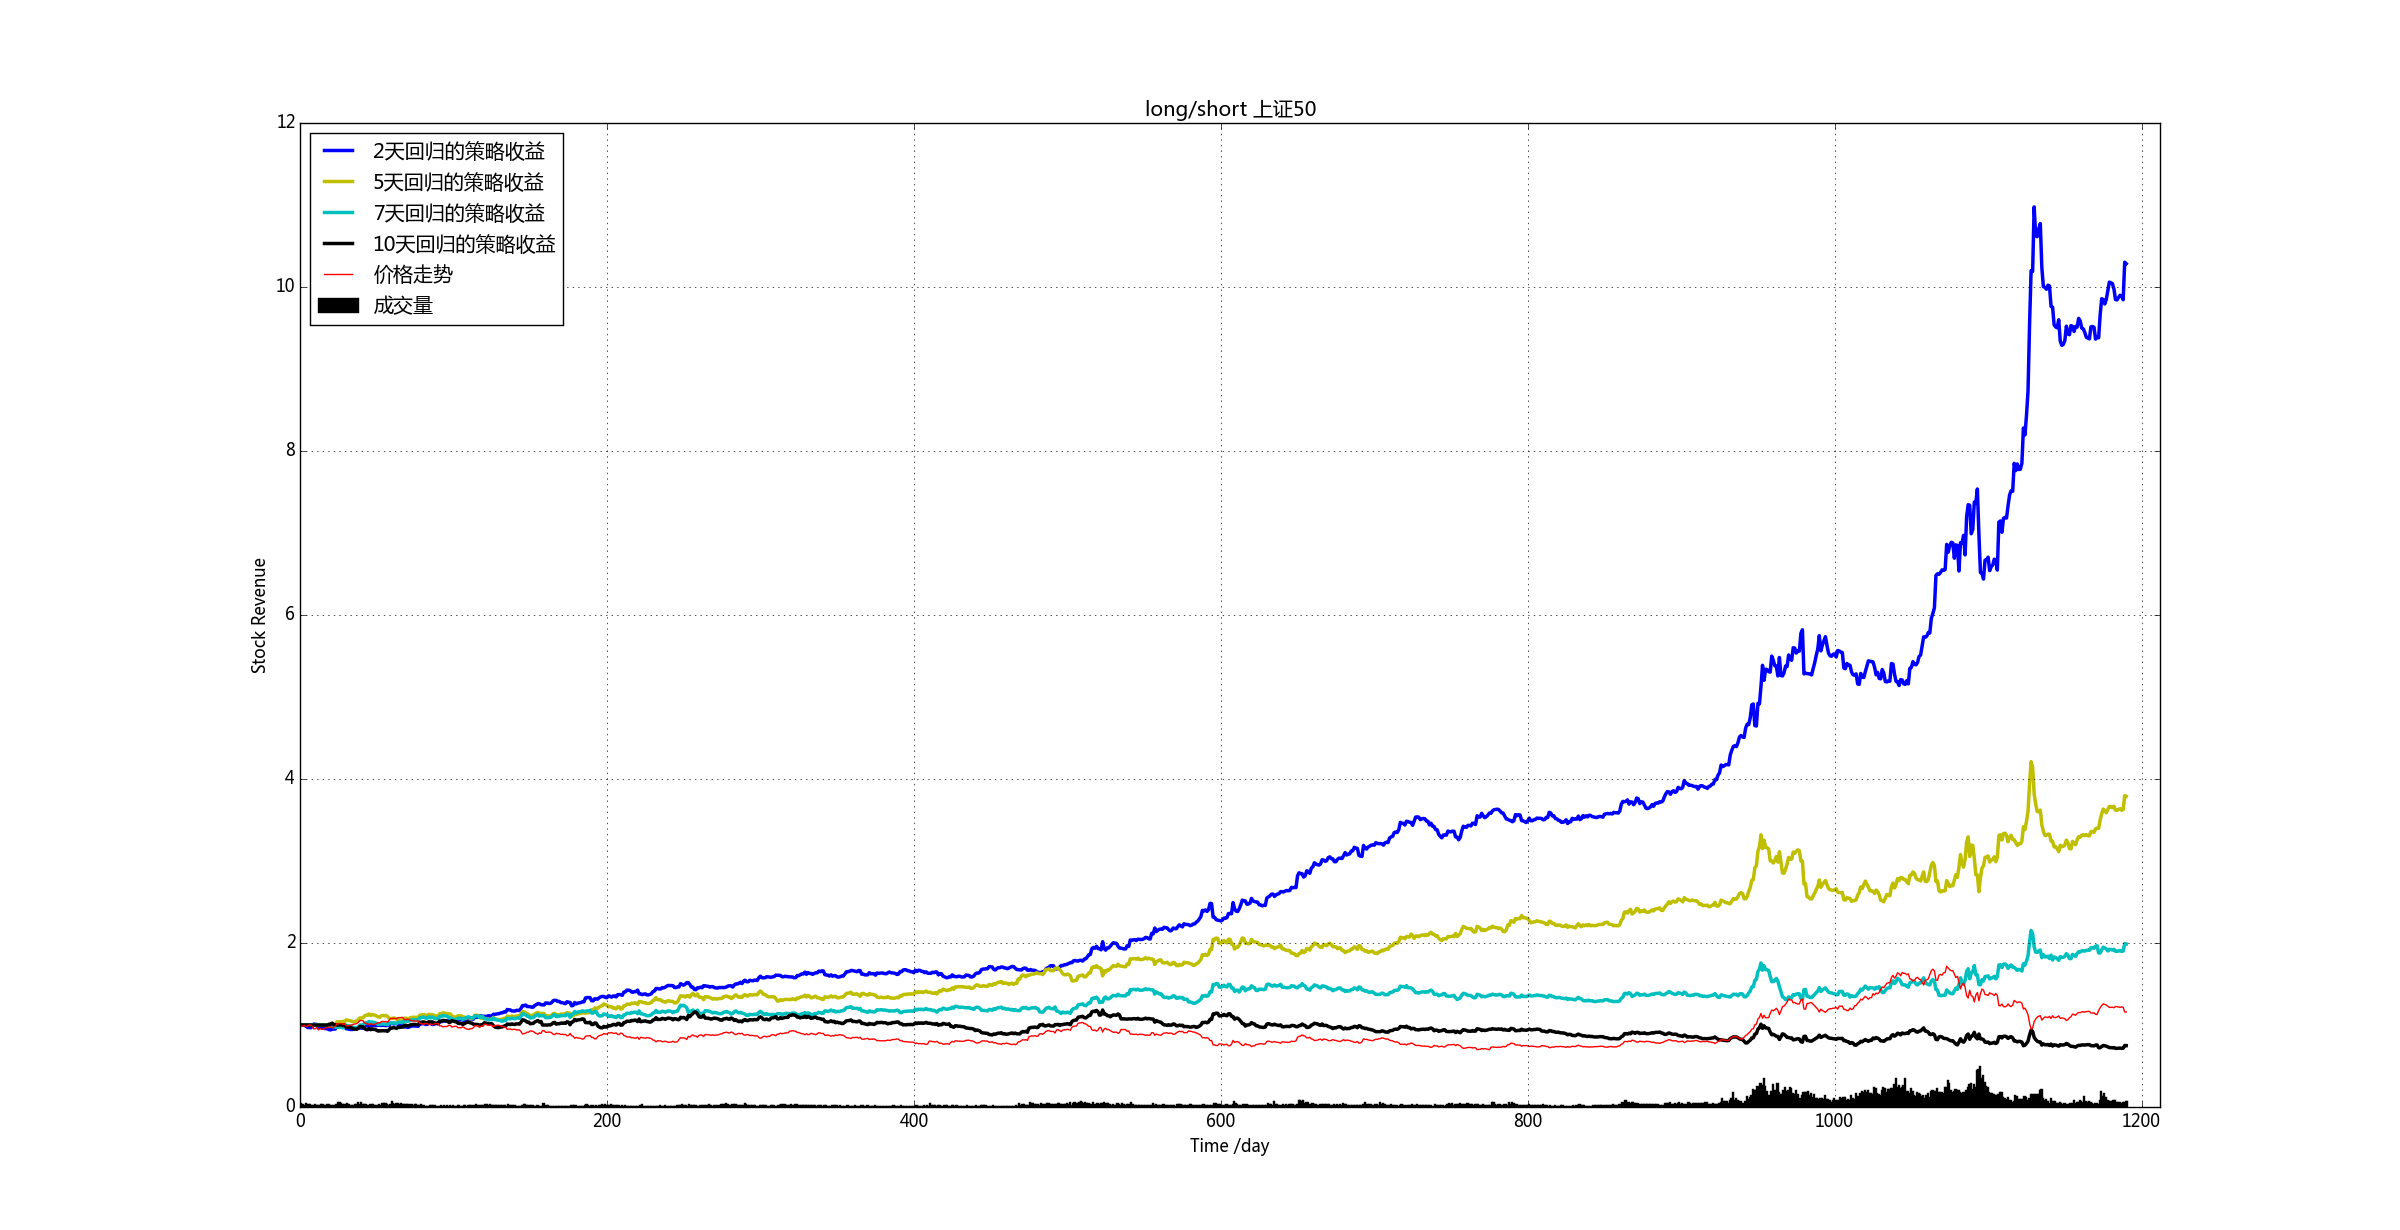
\includegraphics[width=1.0\textwidth]{img_r_1/sz50.png}
	\caption{上证50 long/short}
\end{figure}

\item long/hold 
\begin{figure}[H]
	\centering
	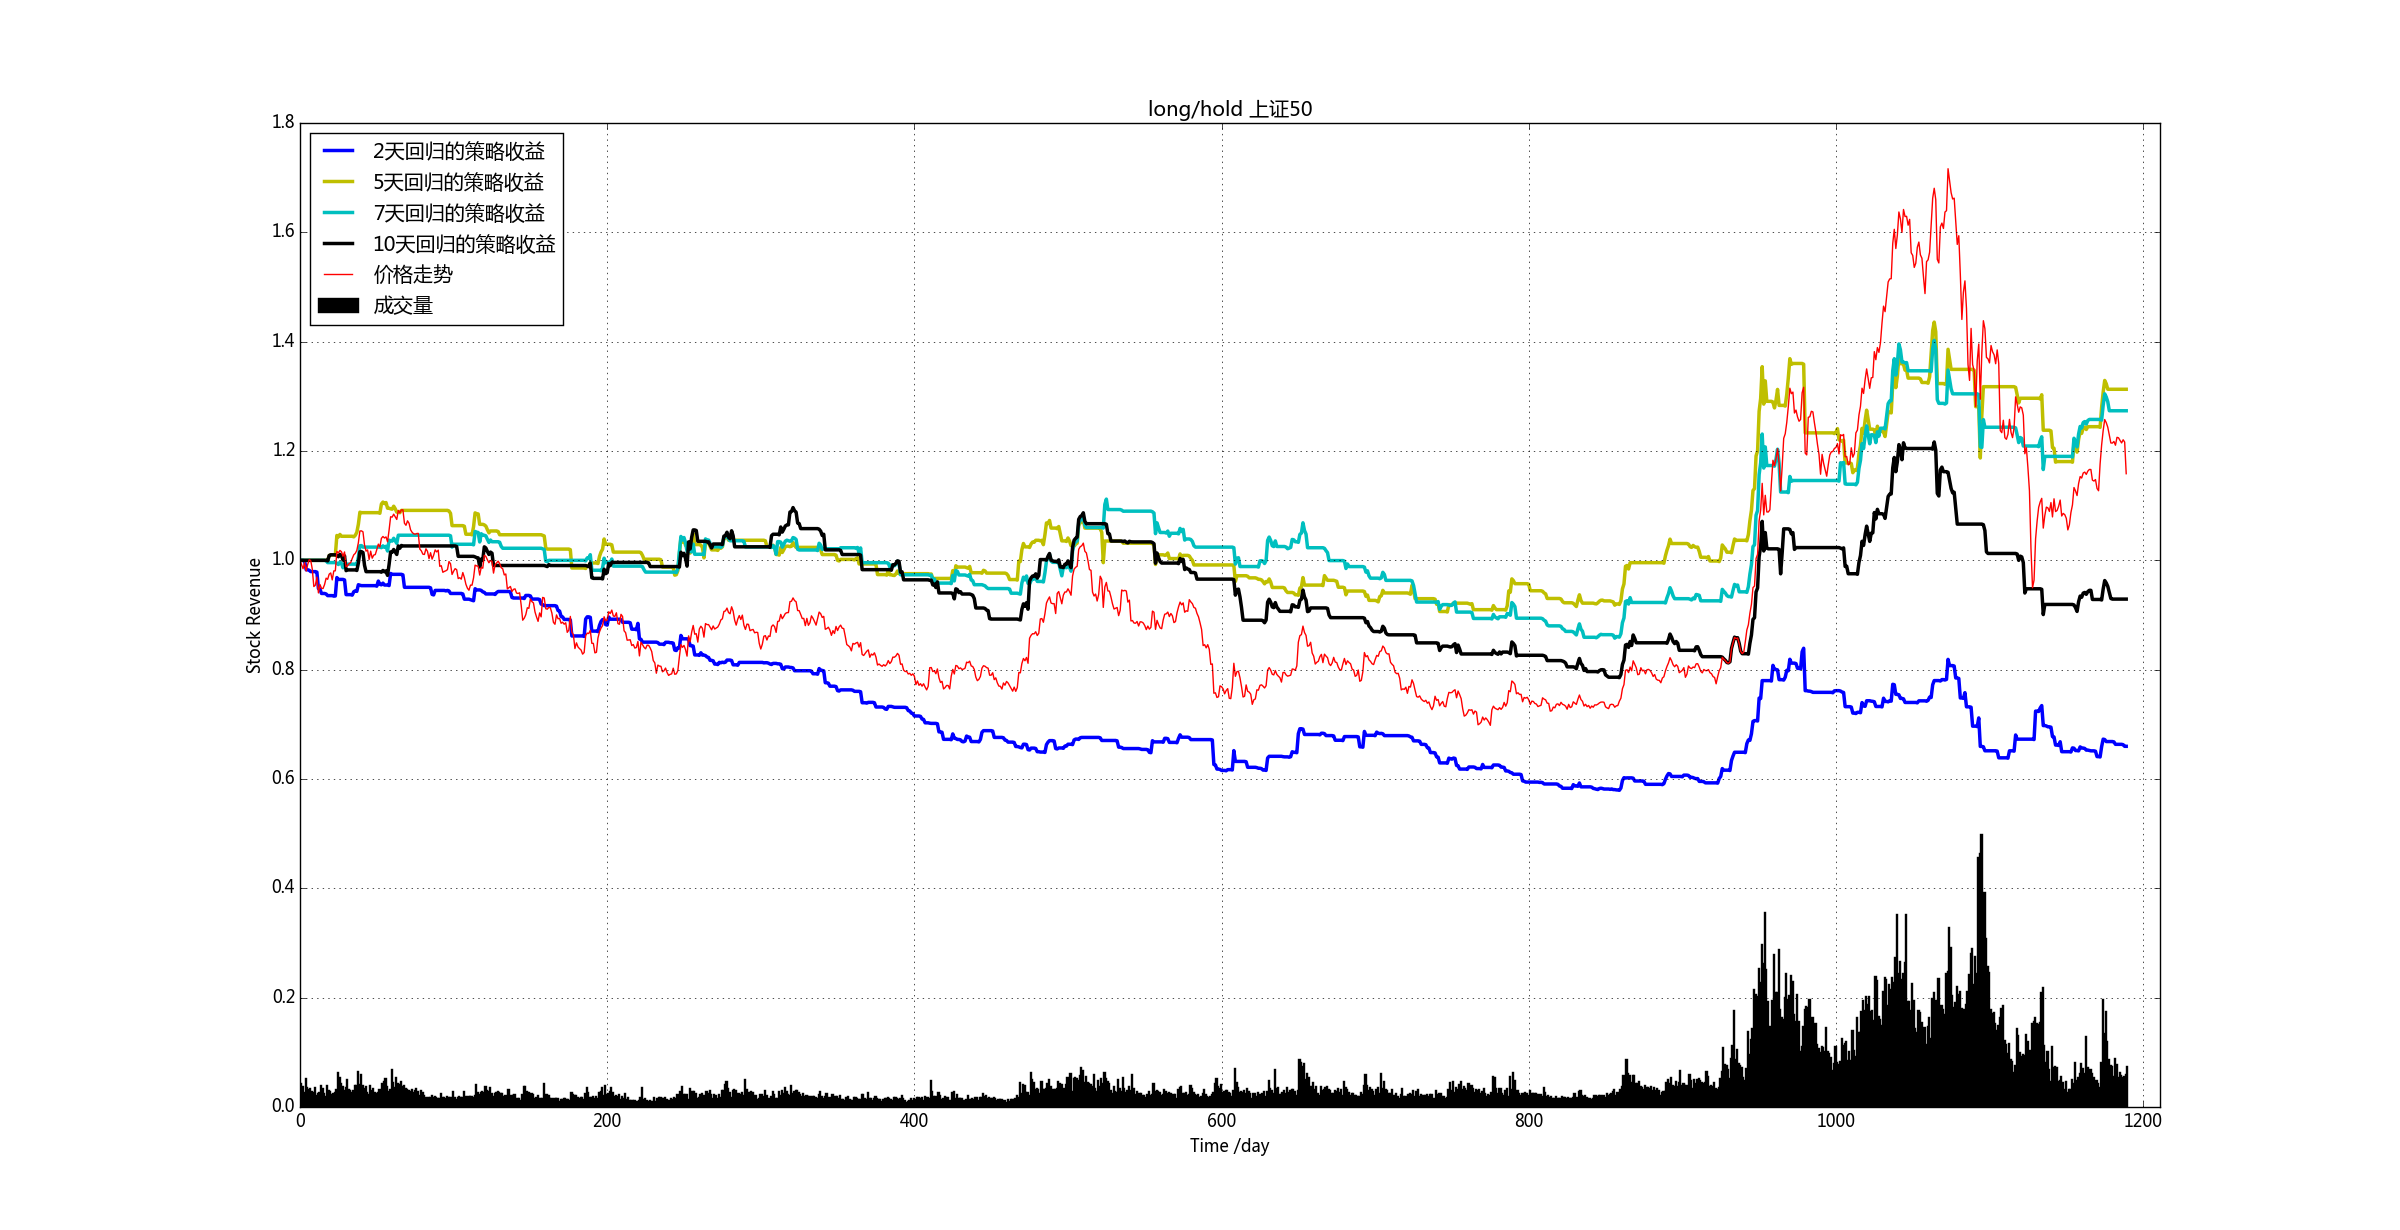
\includegraphics[width=1.0\textwidth]{img_r_1/sz50_1.png}
	\caption{上证50 long/hold}
\end{figure}
\end{enumerate}

\subsubsection{上证综指}

\begin{enumerate}
\item long/short 
\begin{figure}[H]
	\centering
	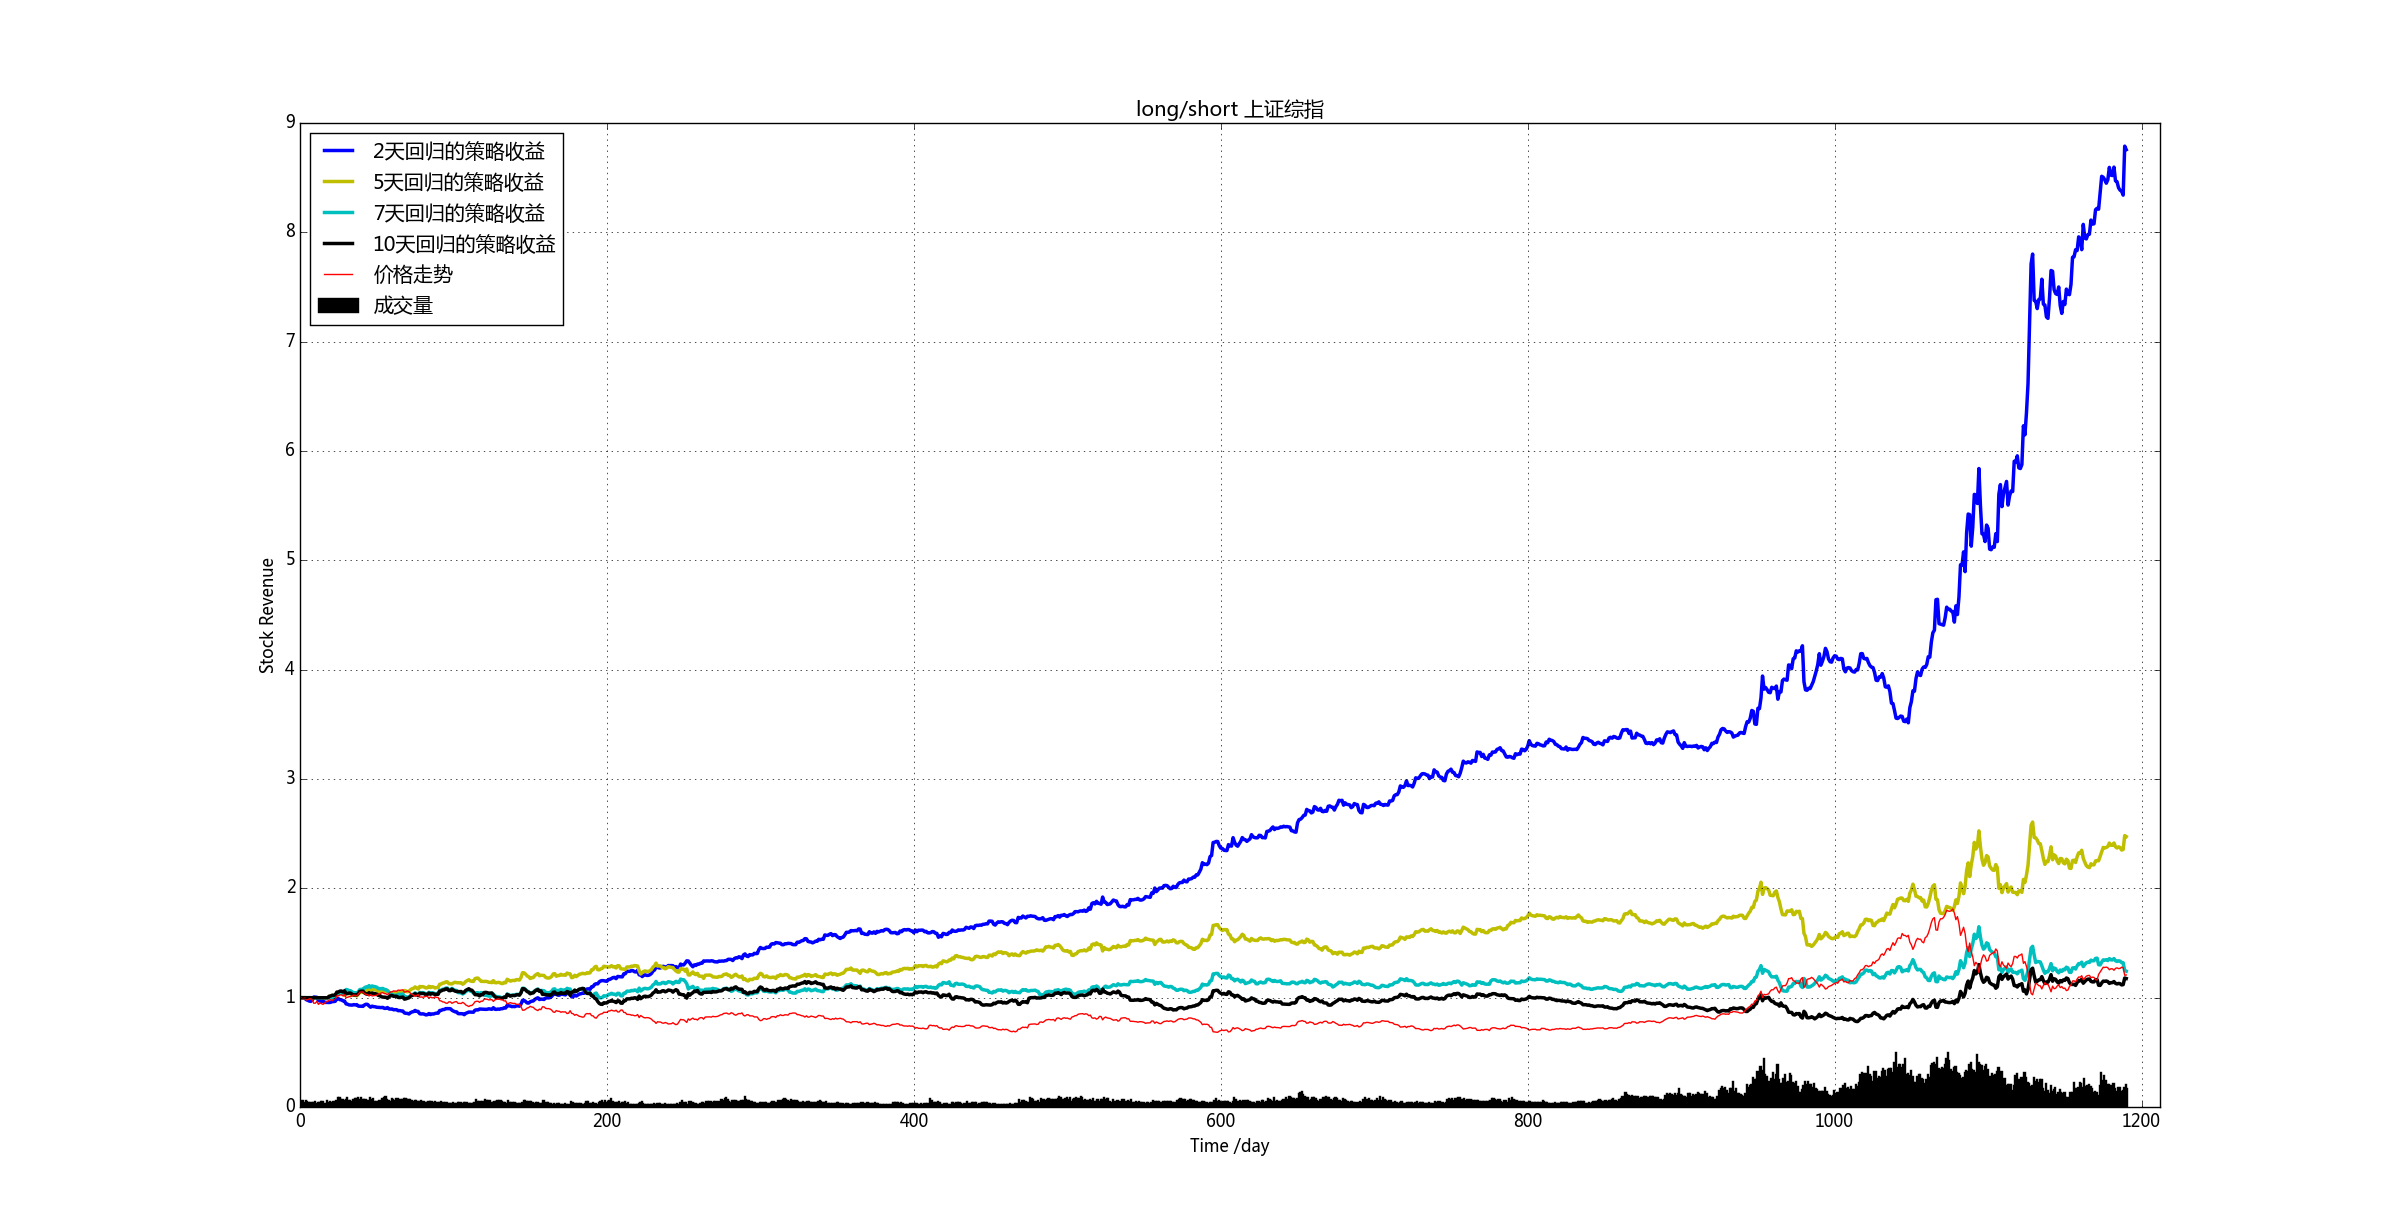
\includegraphics[width=1.0\textwidth]{img_r_1/szzz.png}
	\caption{上证综指 long/short}
\end{figure}
\item long/hold 
\begin{figure}[H]
	\centering
	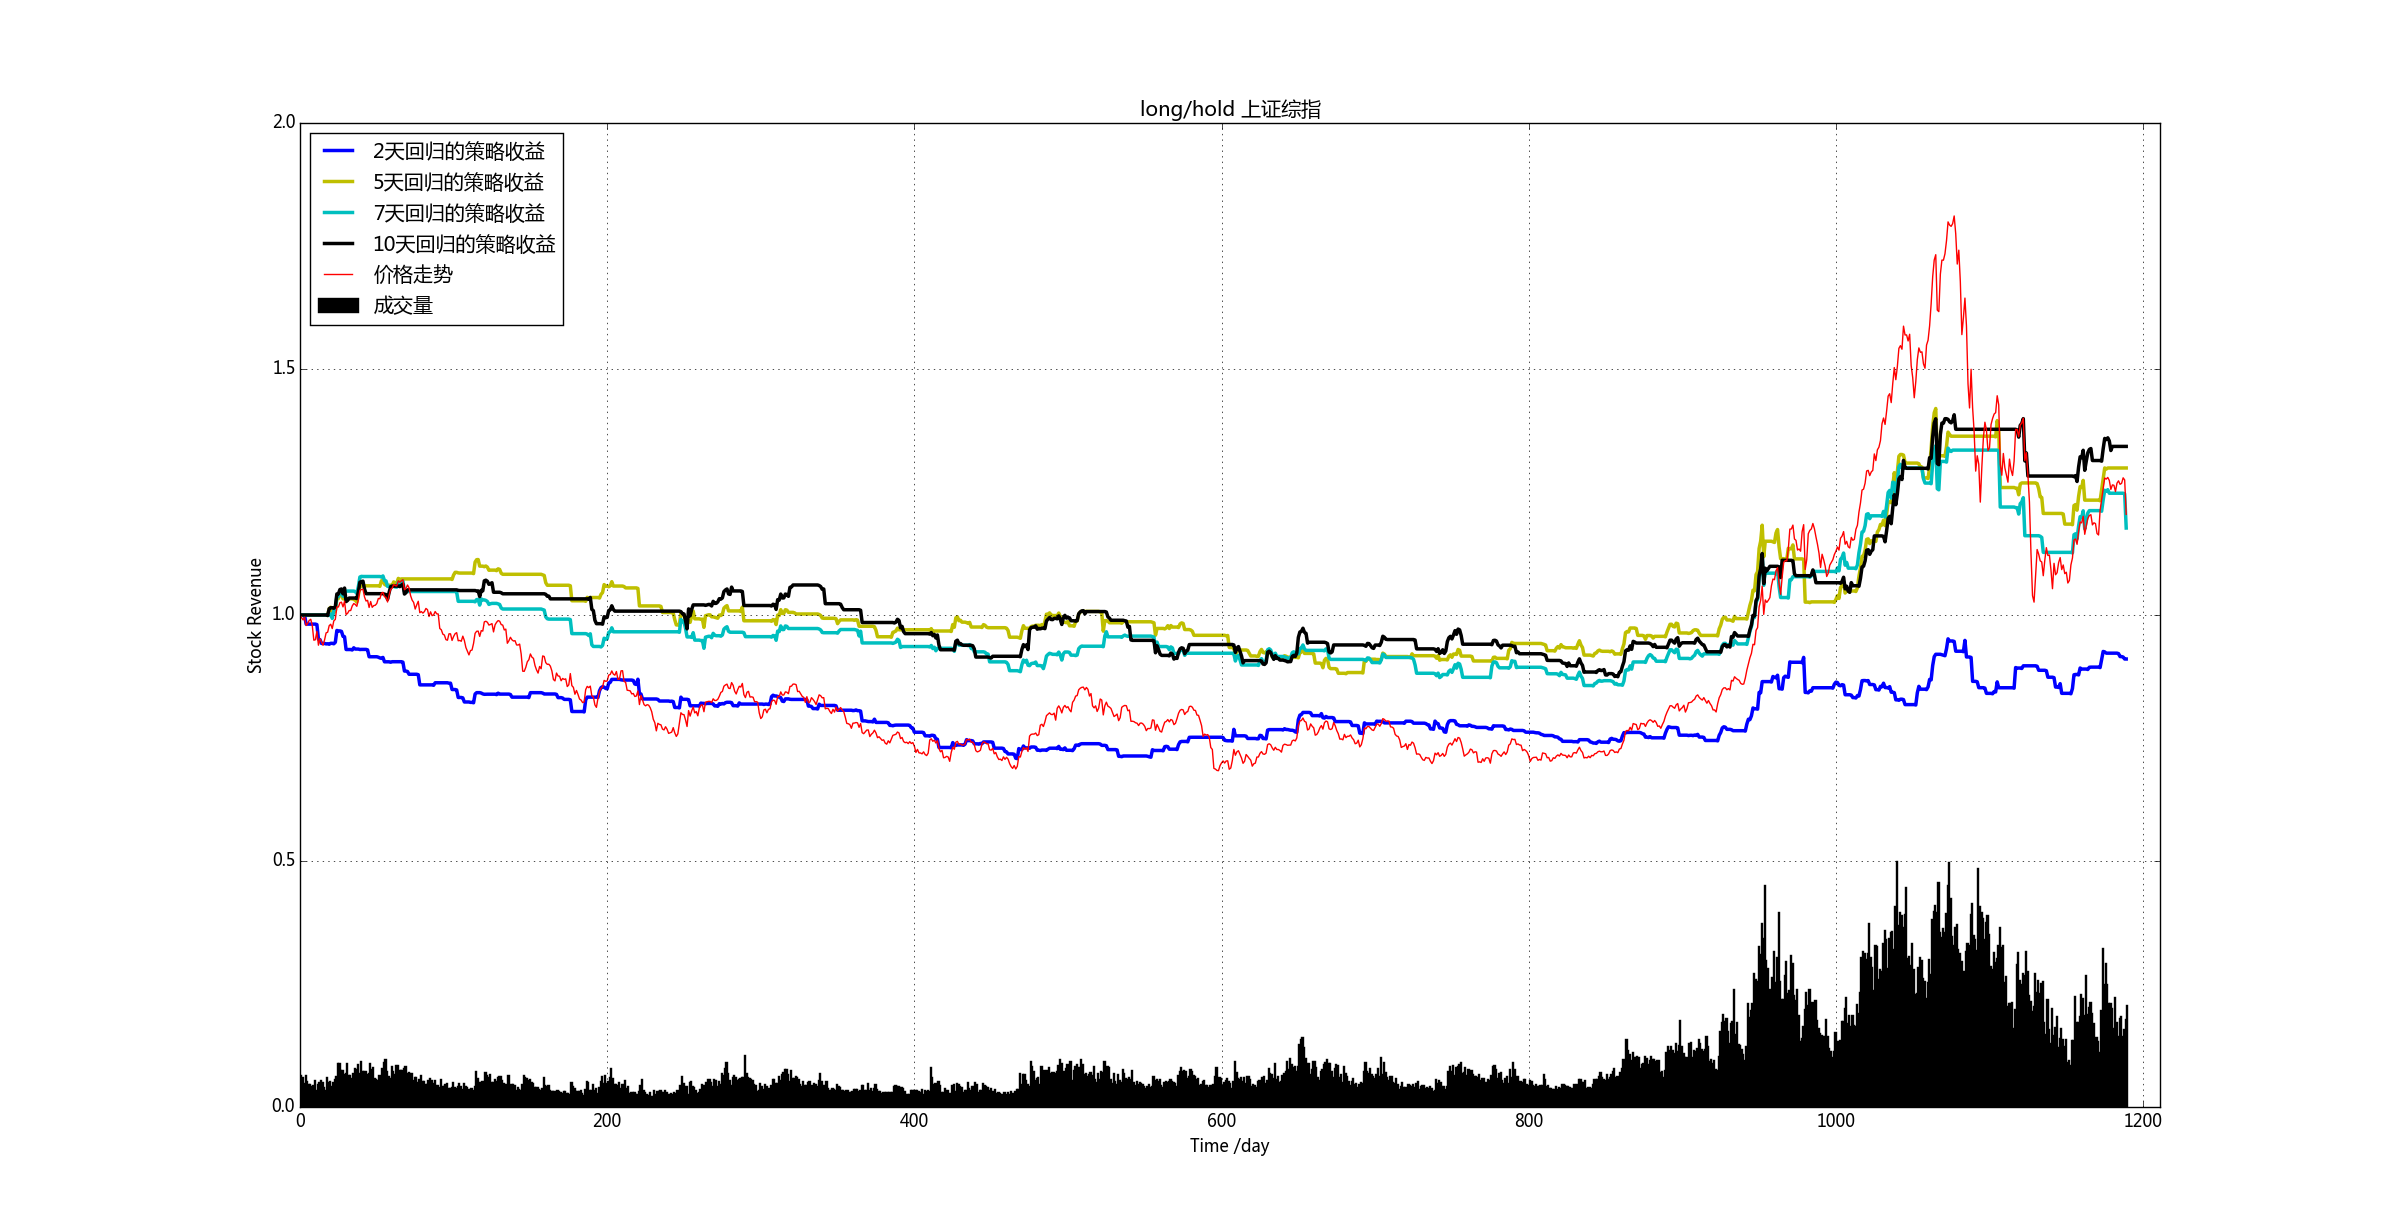
\includegraphics[width=1.0\textwidth]{img_r_1/szzz_1.png}
	\caption{上证综指 long/hold}
\end{figure}
\end{enumerate}

\subsubsection{沪深300}
\begin{enumerate}
\item long/short 
\begin{figure}[H]
	\centering
	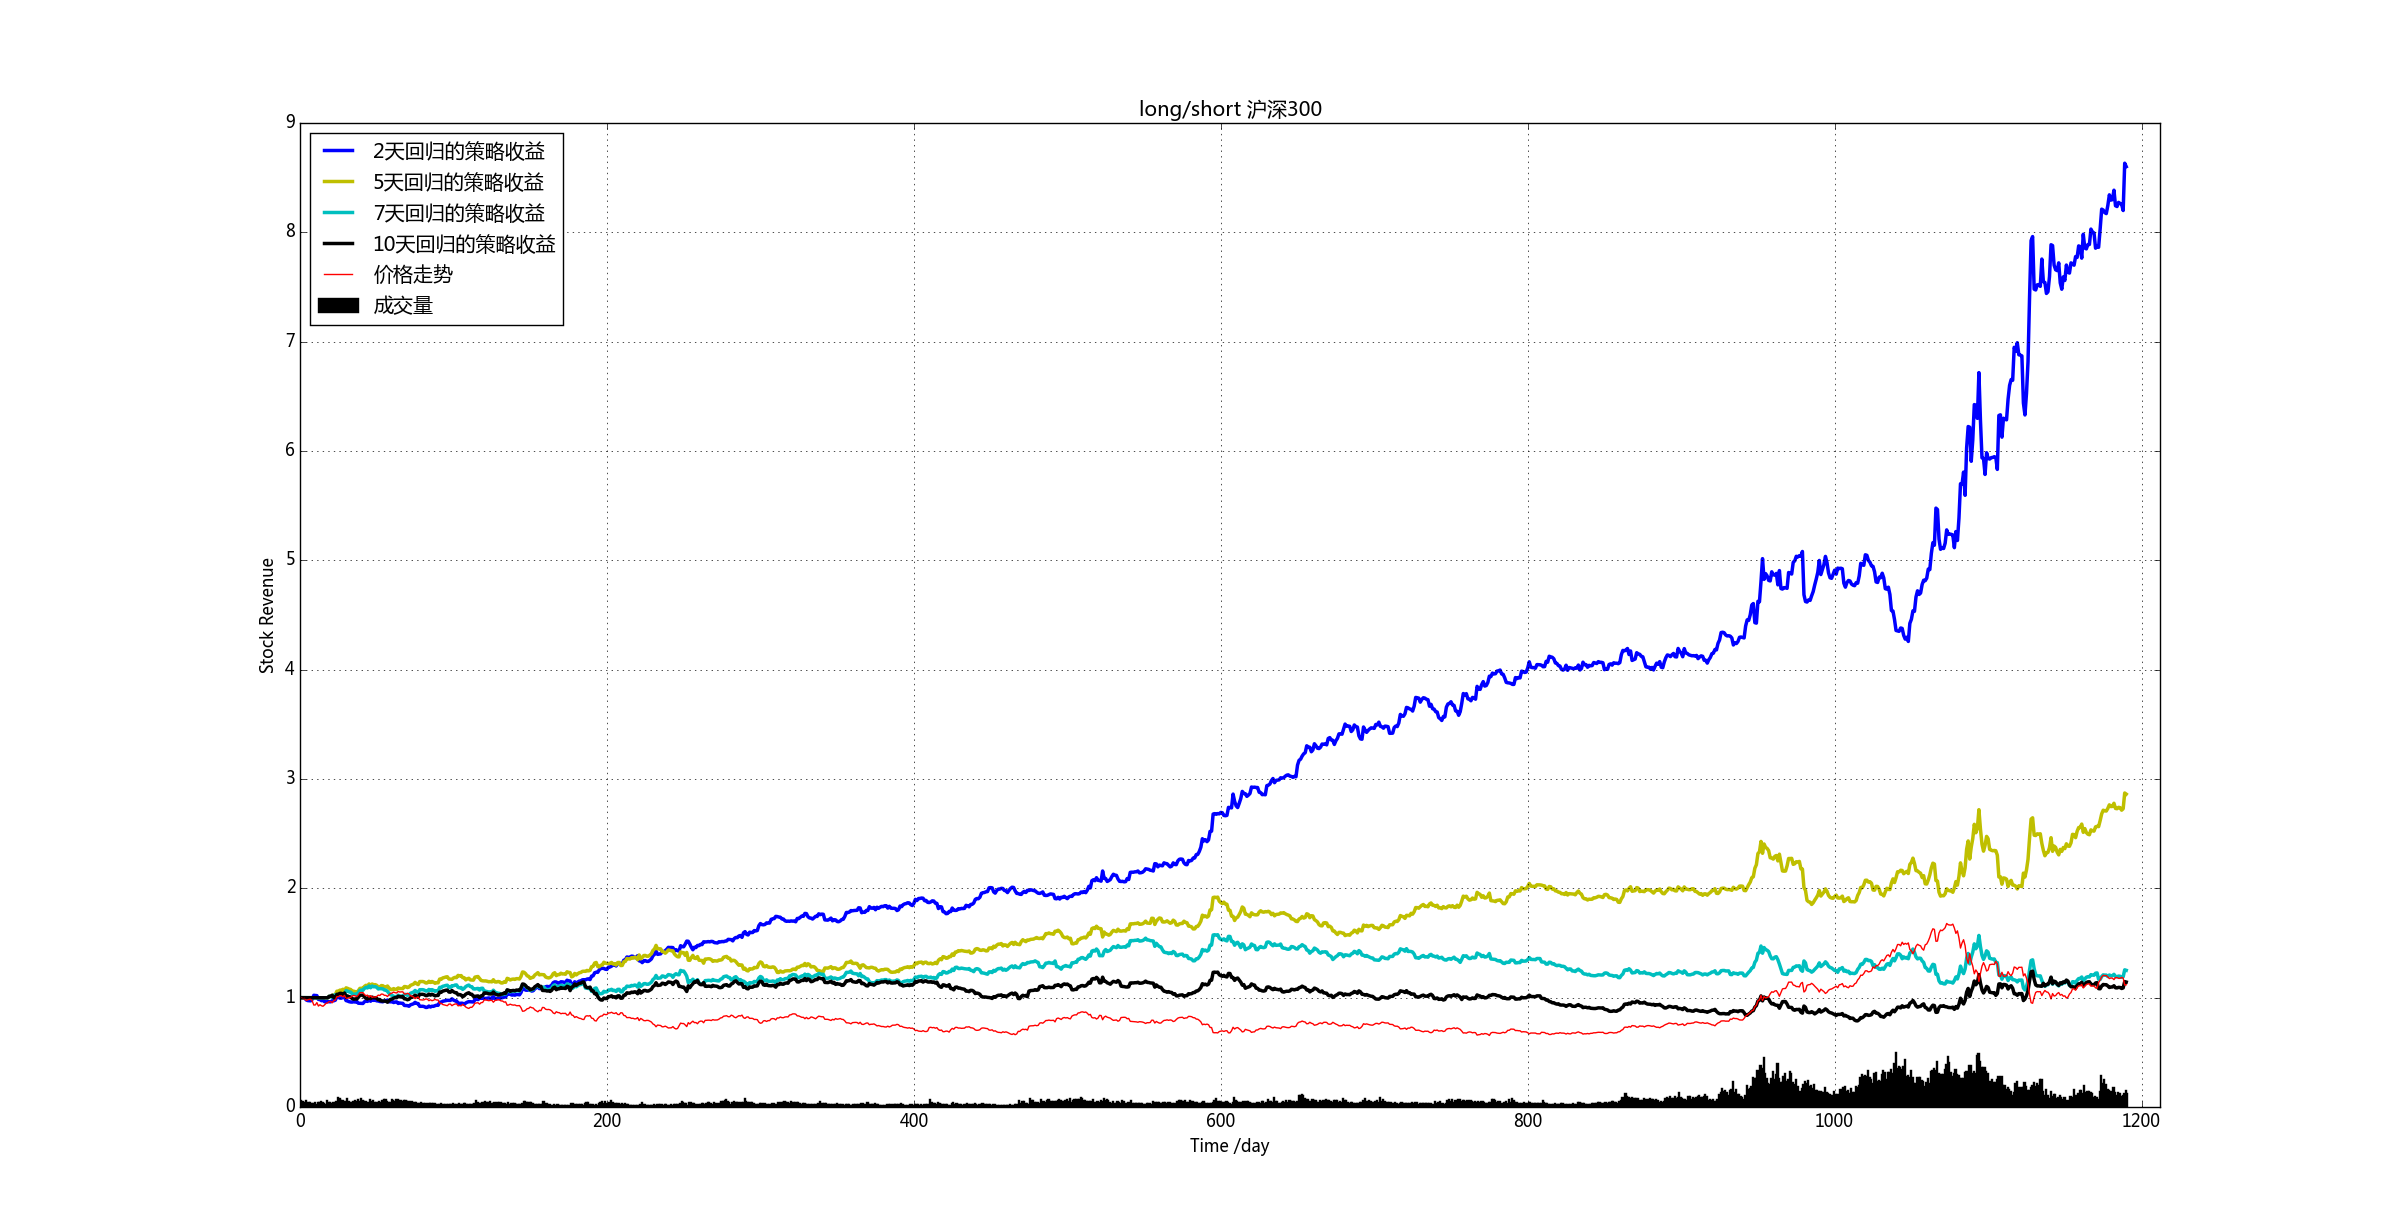
\includegraphics[width=1.0\textwidth]{img_r_1/hs300.png}
	\caption{沪深300 long/short }
\end{figure}
\item long/hold 
\begin{figure}[H]
	\centering
	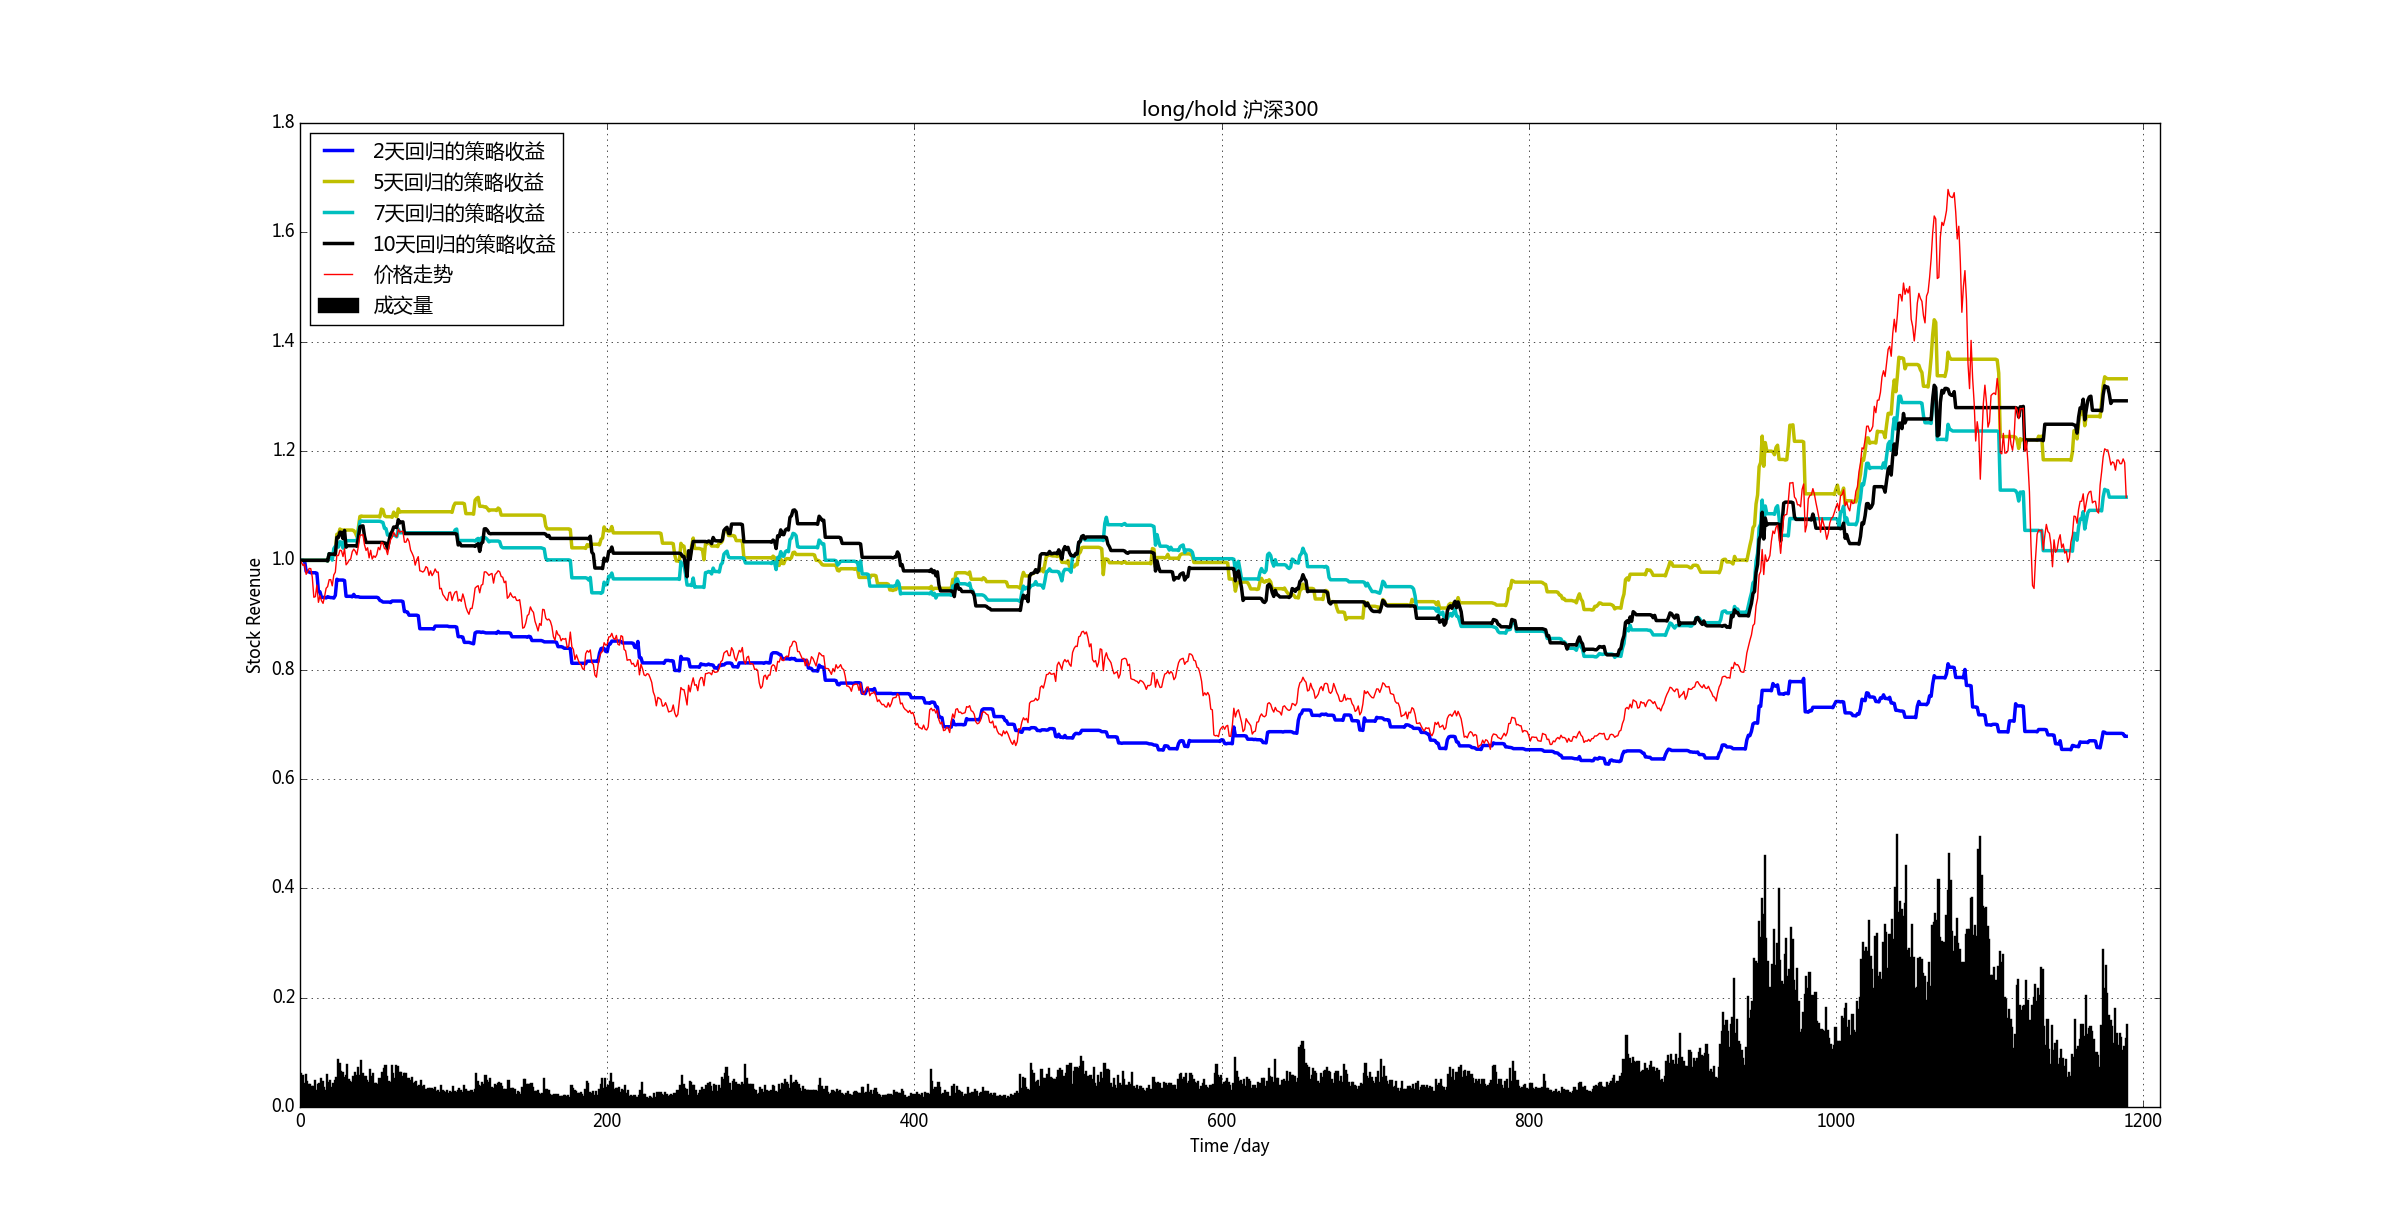
\includegraphics[width=1.0\textwidth]{img_r_1/hs300_1.png}
	\caption{沪深300 long/hold }
\end{figure}
\end{enumerate}

\subsubsection{创业板}
\begin{enumerate}
\item long/short 
\begin{figure}[H]
	\centering
	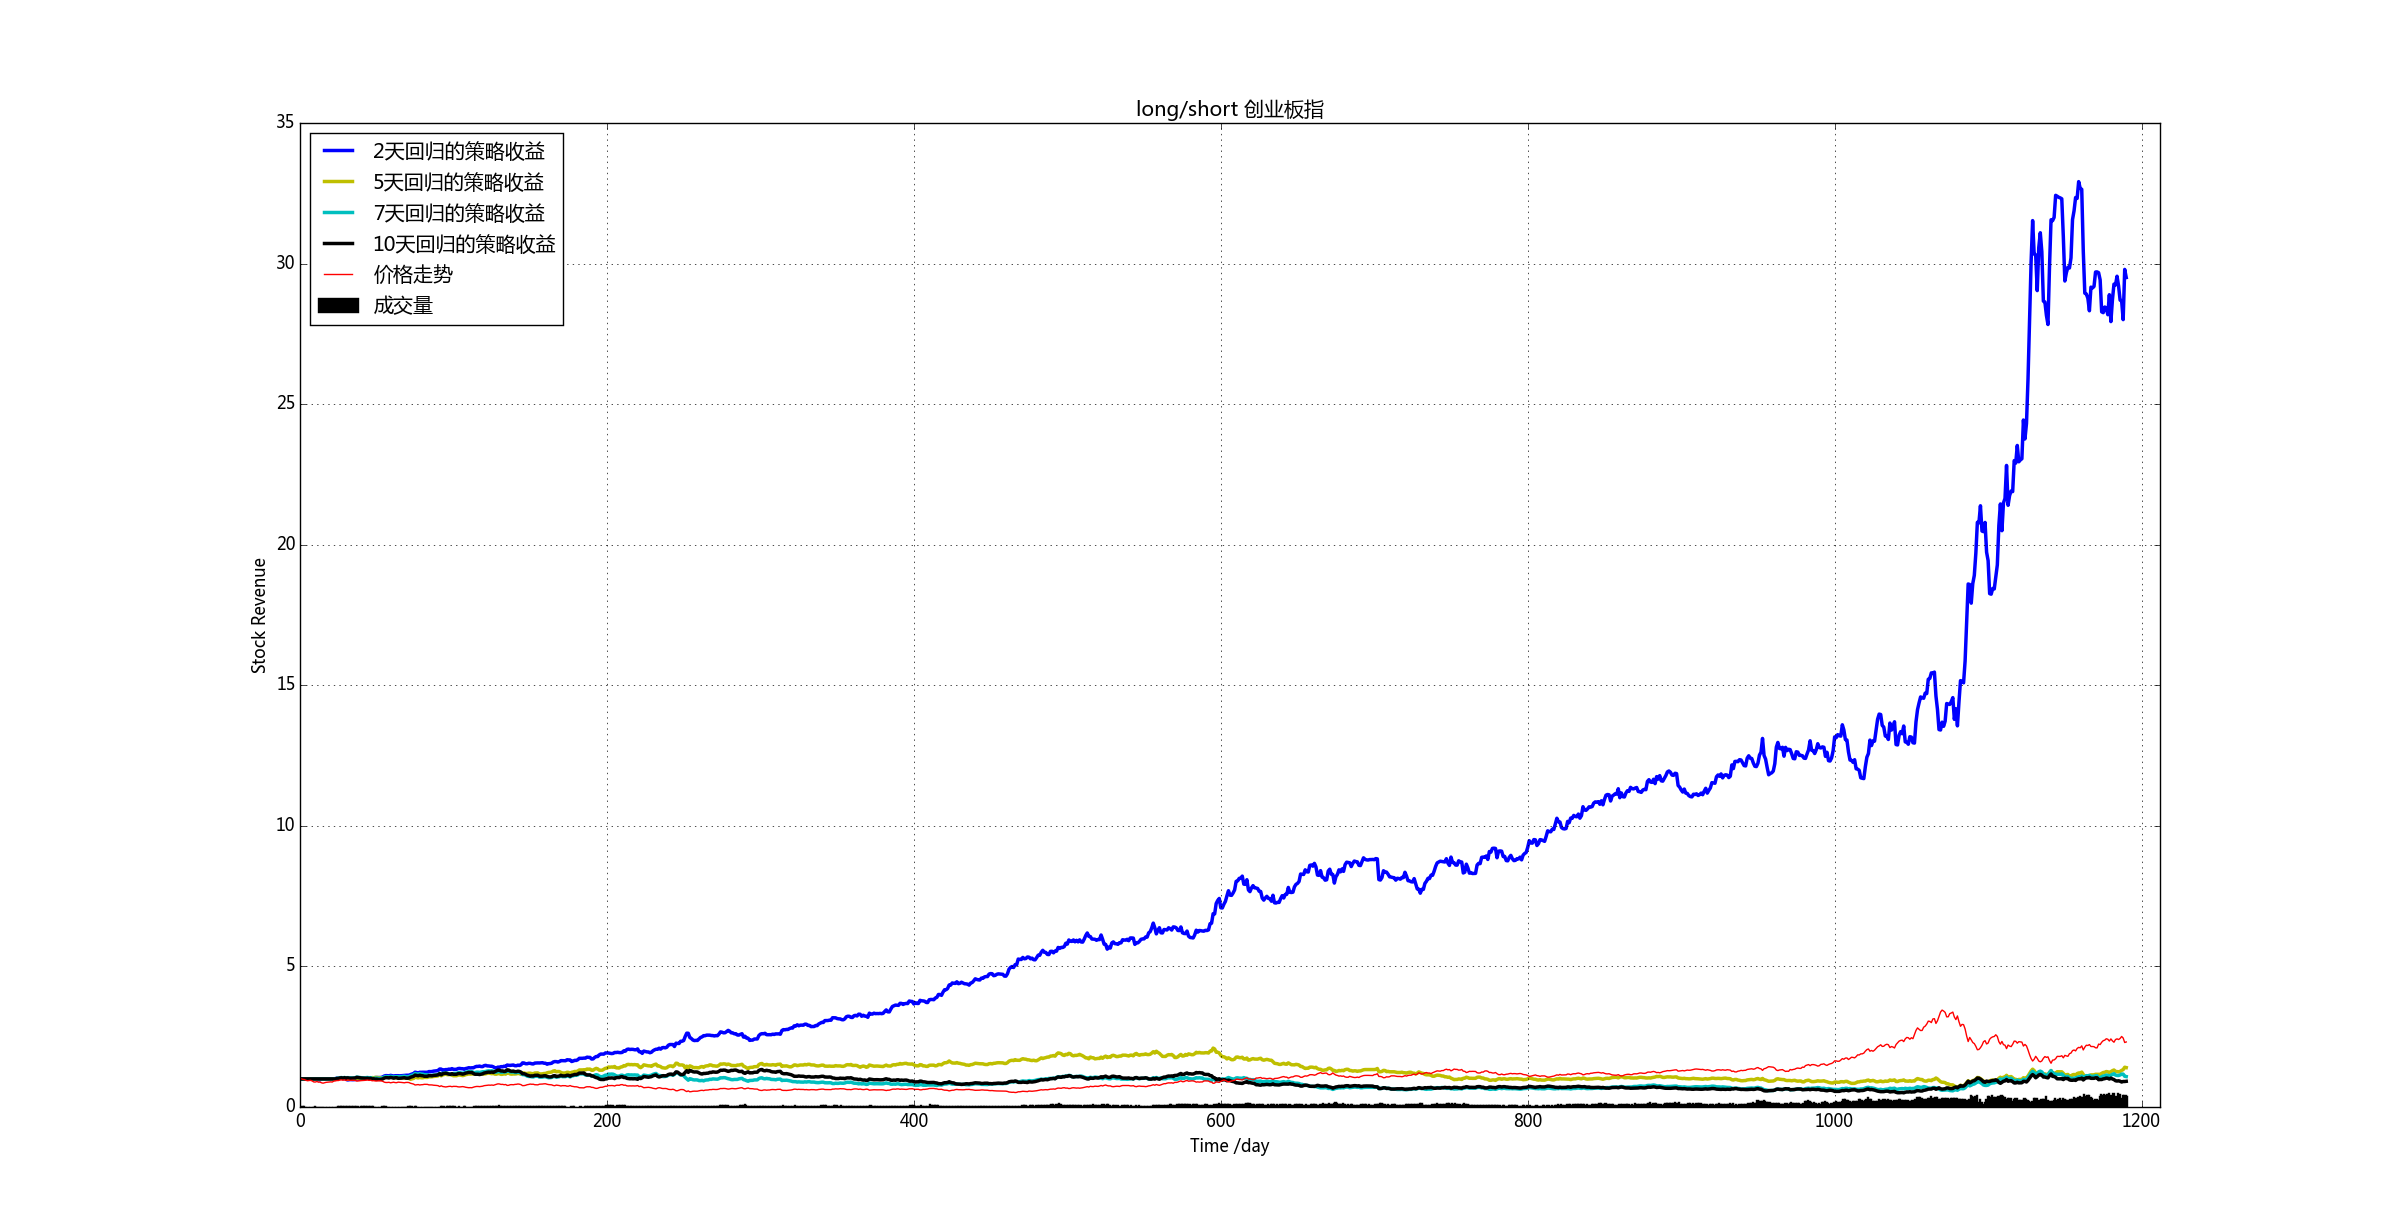
\includegraphics[width=1.0\textwidth]{img_r_1/cyb.png}
	\caption{创业板 long/short}
\end{figure}
\item long/hold 
\begin{figure}[H]
	\centering
	\includegraphics[width=1.0\textwidth]{img_r_1/cyb_1.png}
	\caption{创业板 long/hold }
\end{figure}
\end{enumerate}

\subsubsection{中证500}
\begin{enumerate}
\item long/short 
\begin{figure}[H]
	\centering
	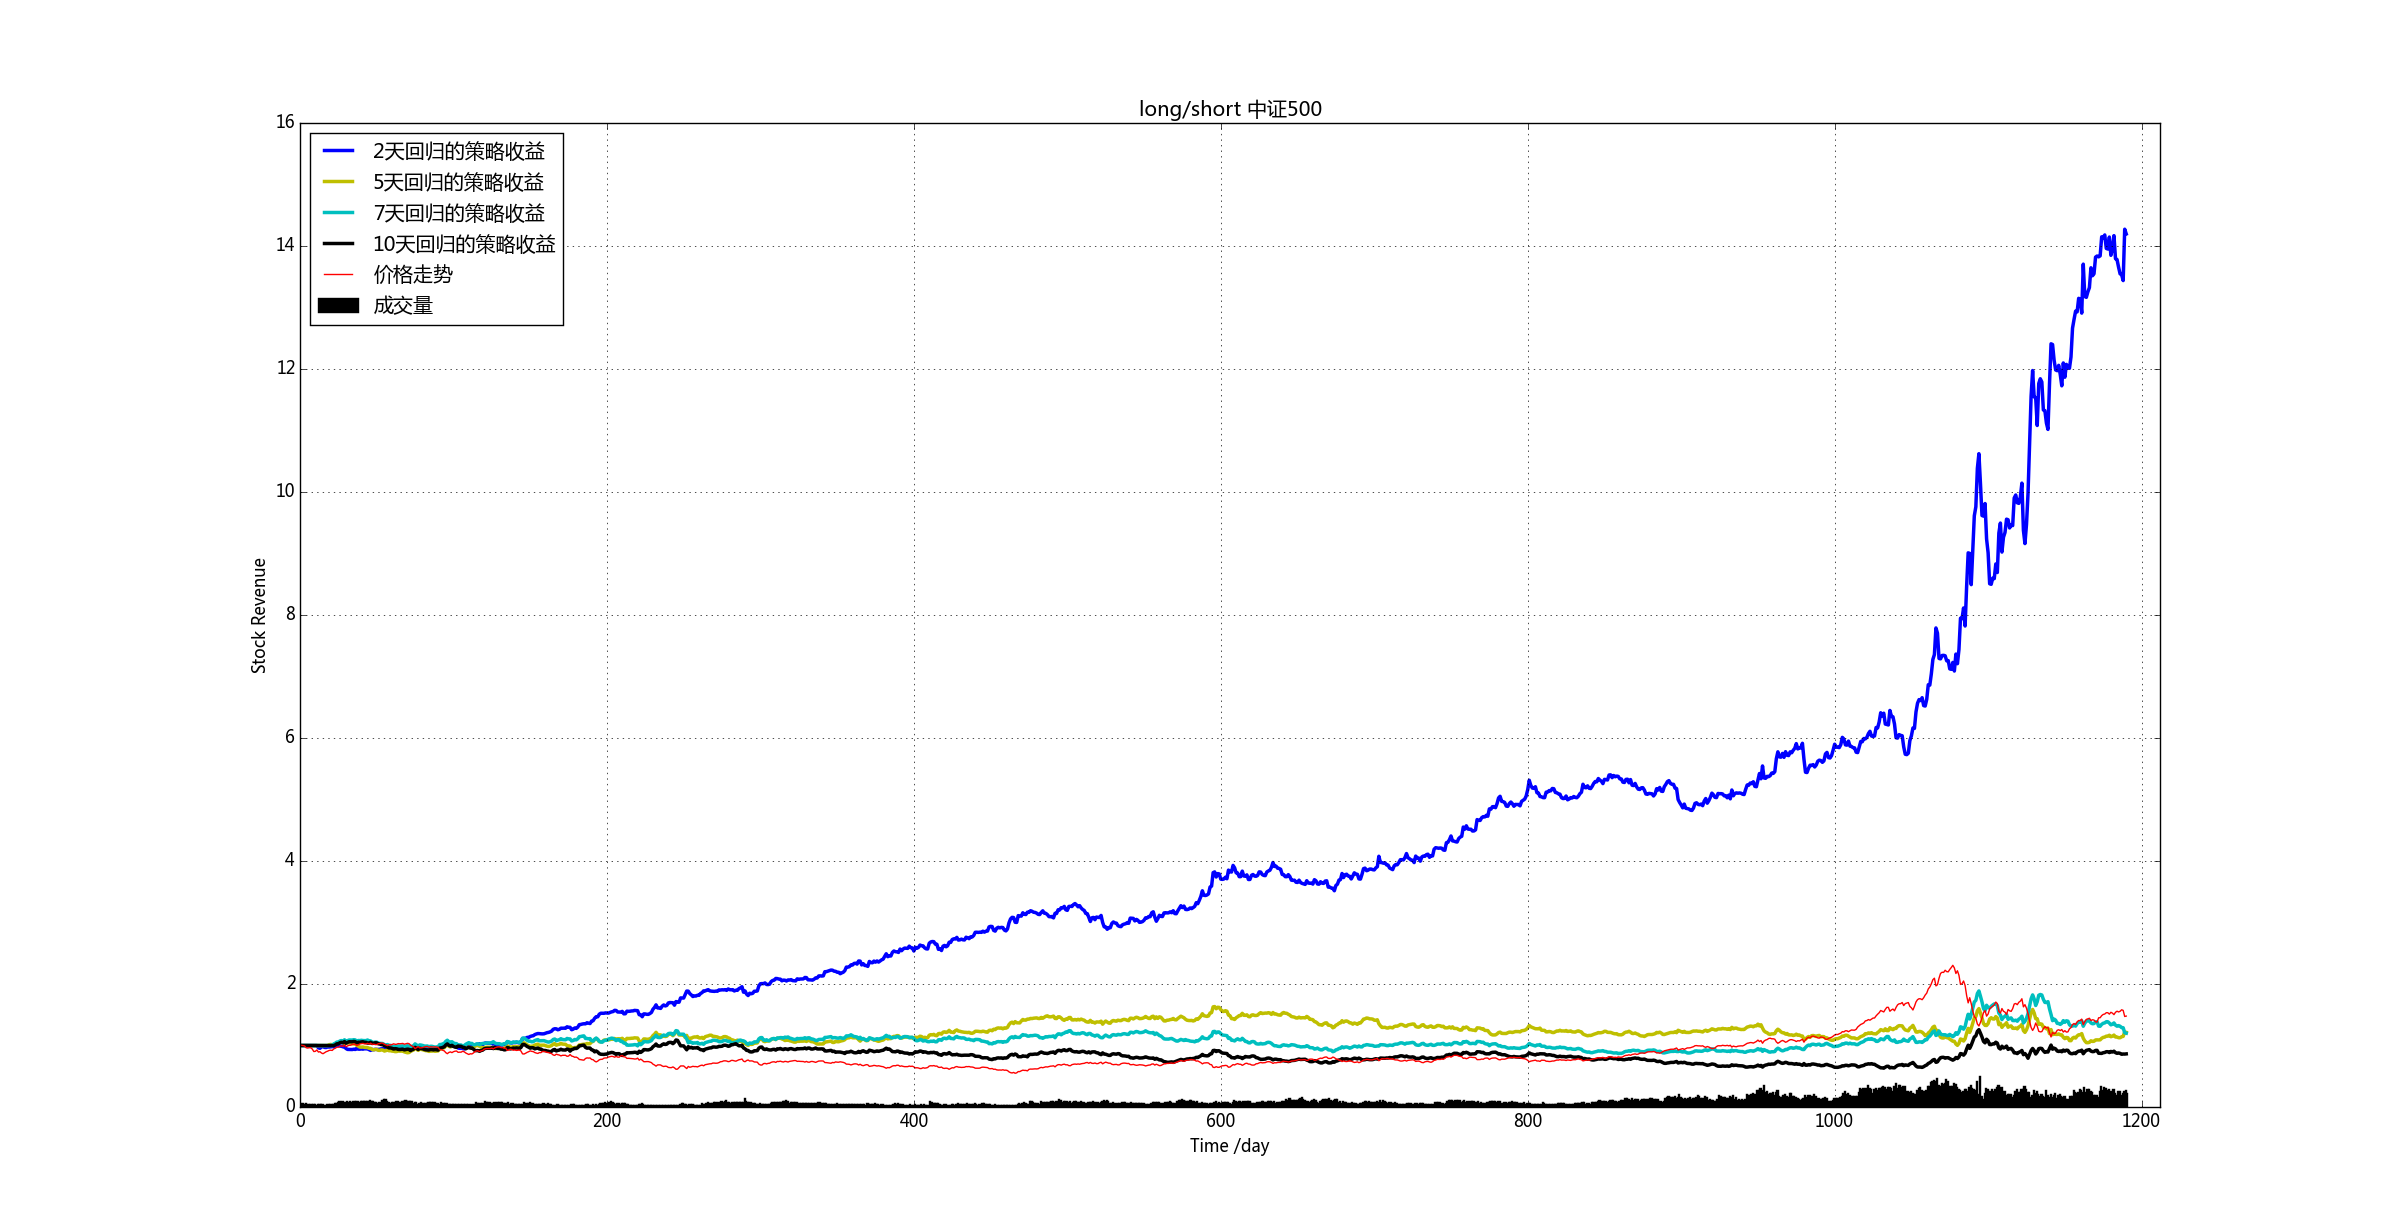
\includegraphics[width=1.0\textwidth]{img_r_1/zz500.png}
	\caption{中证500 long/short }
\end{figure}
\item long/hold 
\begin{figure}[H]
	\centering
	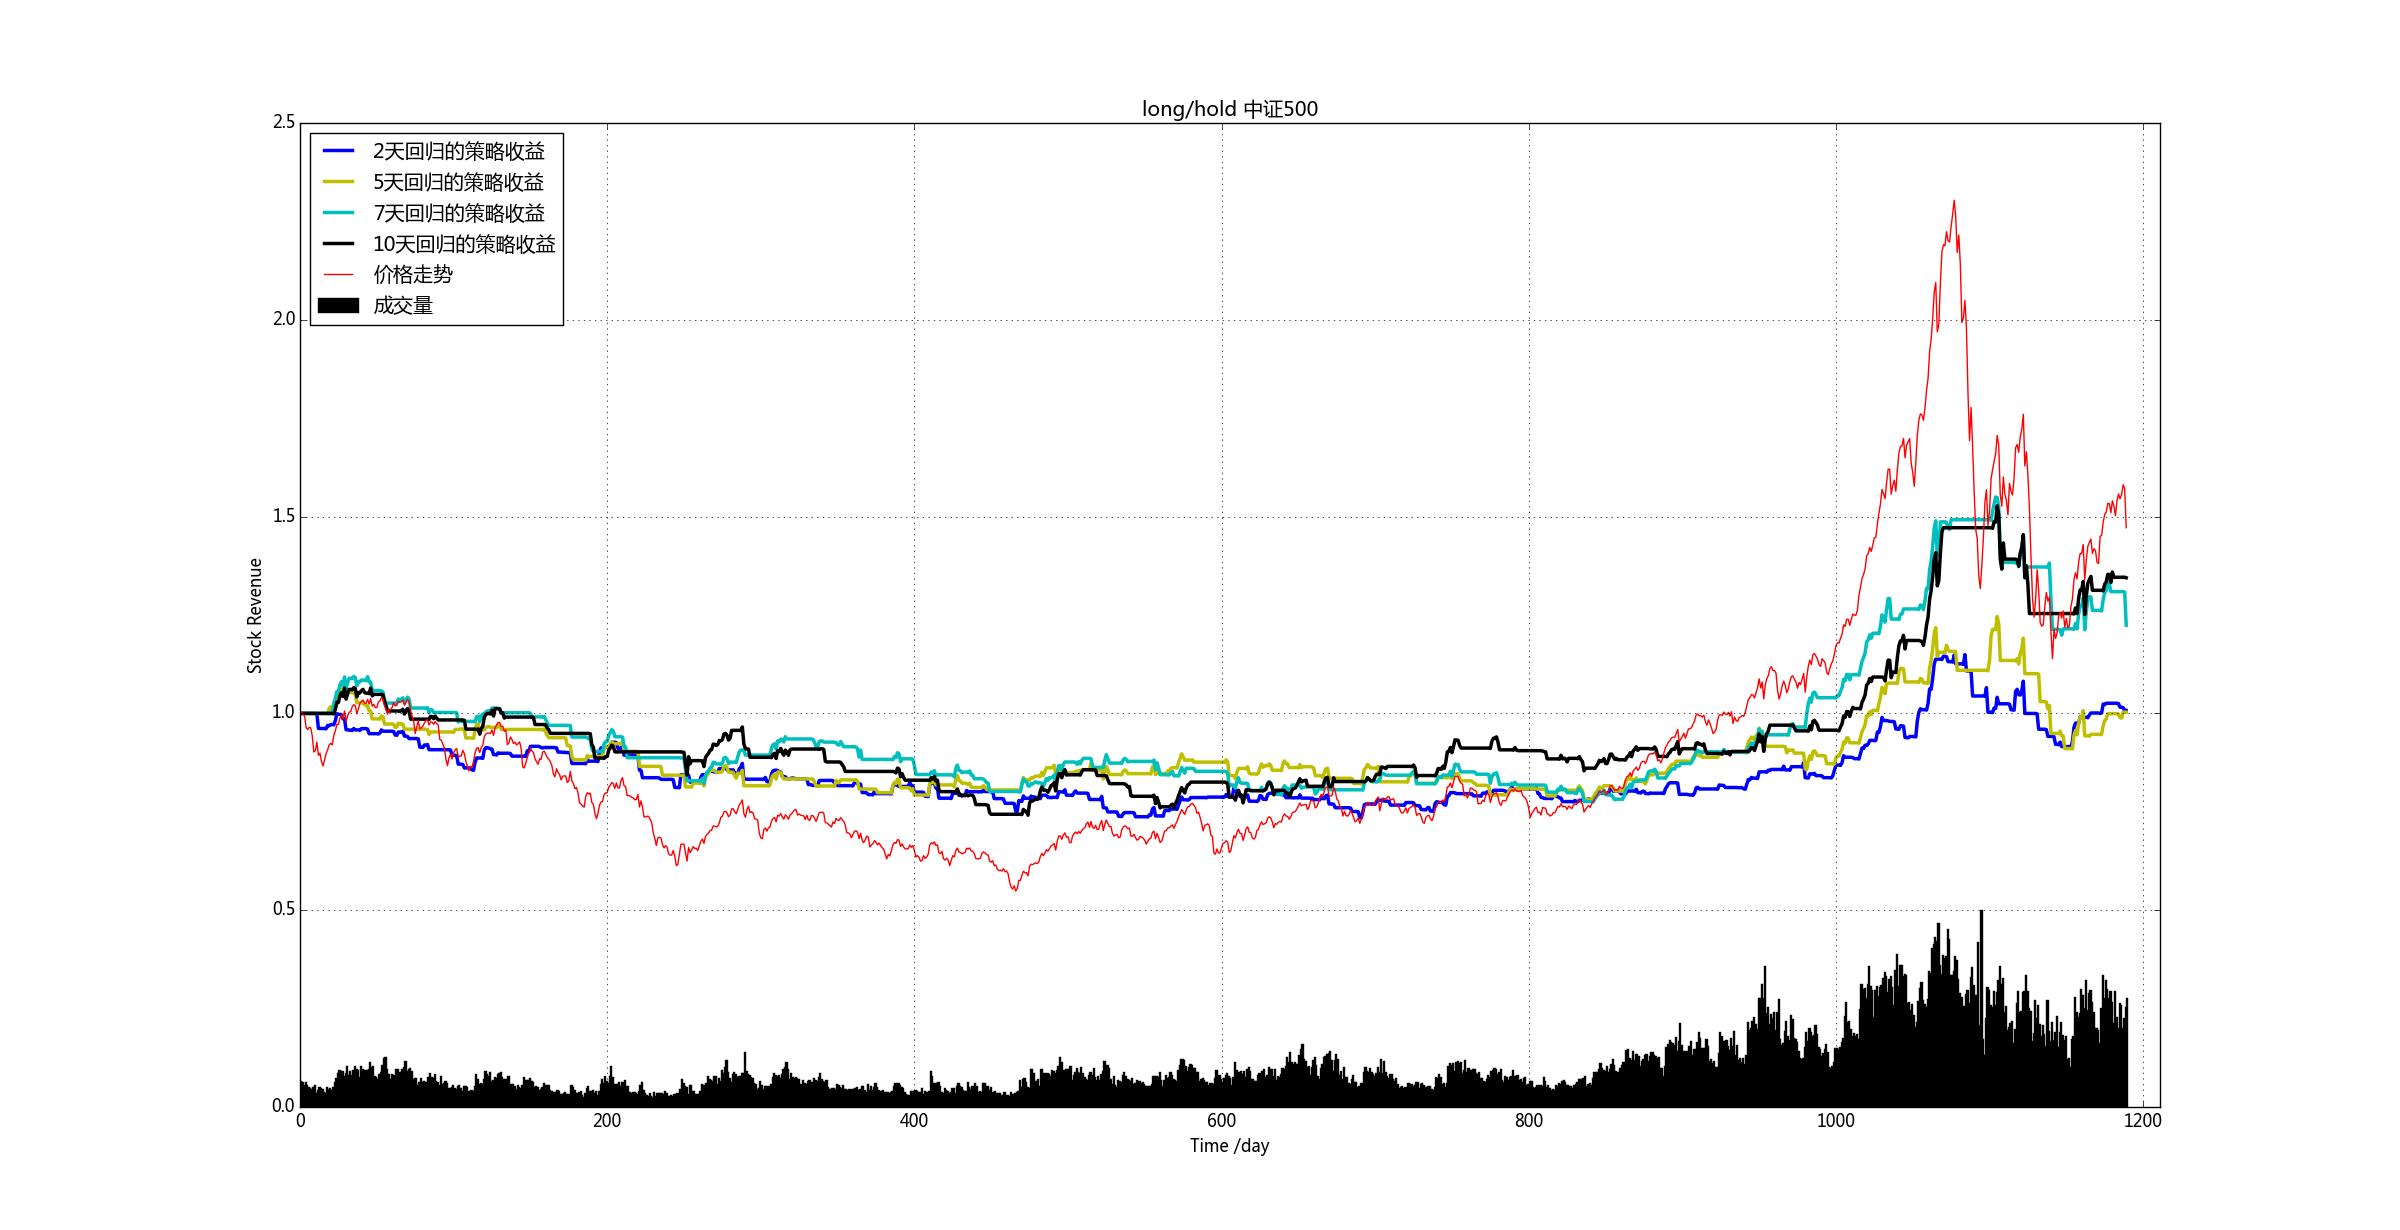
\includegraphics[width=1.0\textwidth]{img_r_1/zz500_1.png}
	\caption{中证500 long/hold}
\end{figure}
\end{enumerate}

\subsection{价格和成交量2日MA}
\subsubsection{上证50}

\begin{enumerate}
\item long/short 
\begin{figure}[H]
	\centering
	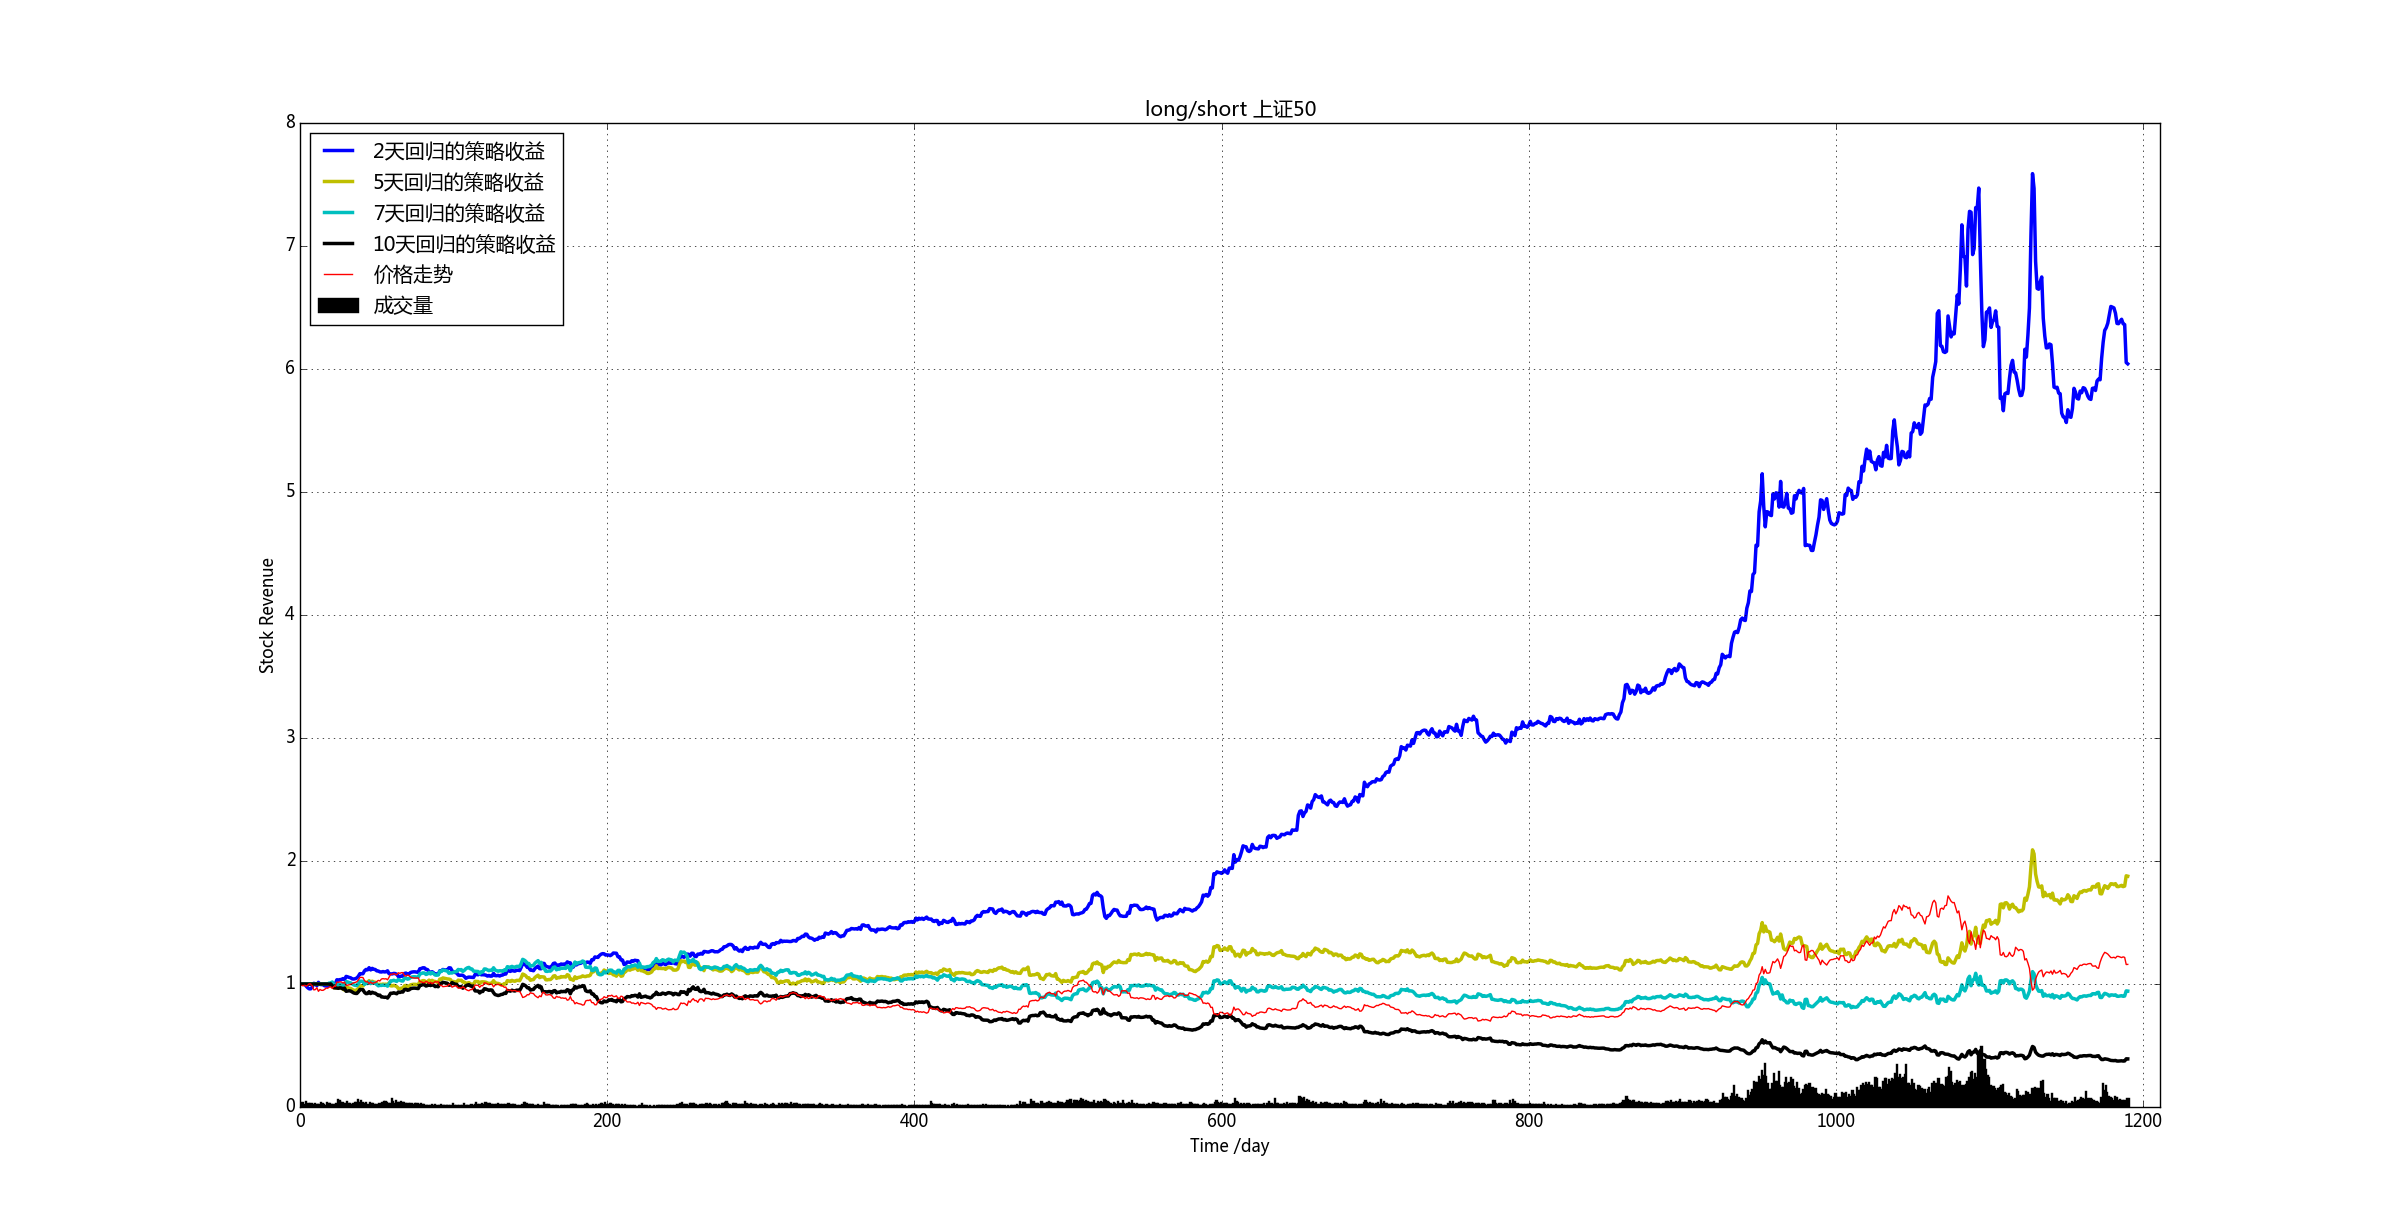
\includegraphics[width=1.0\textwidth]{img_r_2/sz50.png}
	\caption{上证50 long/short}
\end{figure}

\item long/hold 
\begin{figure}[H]
	\centering
	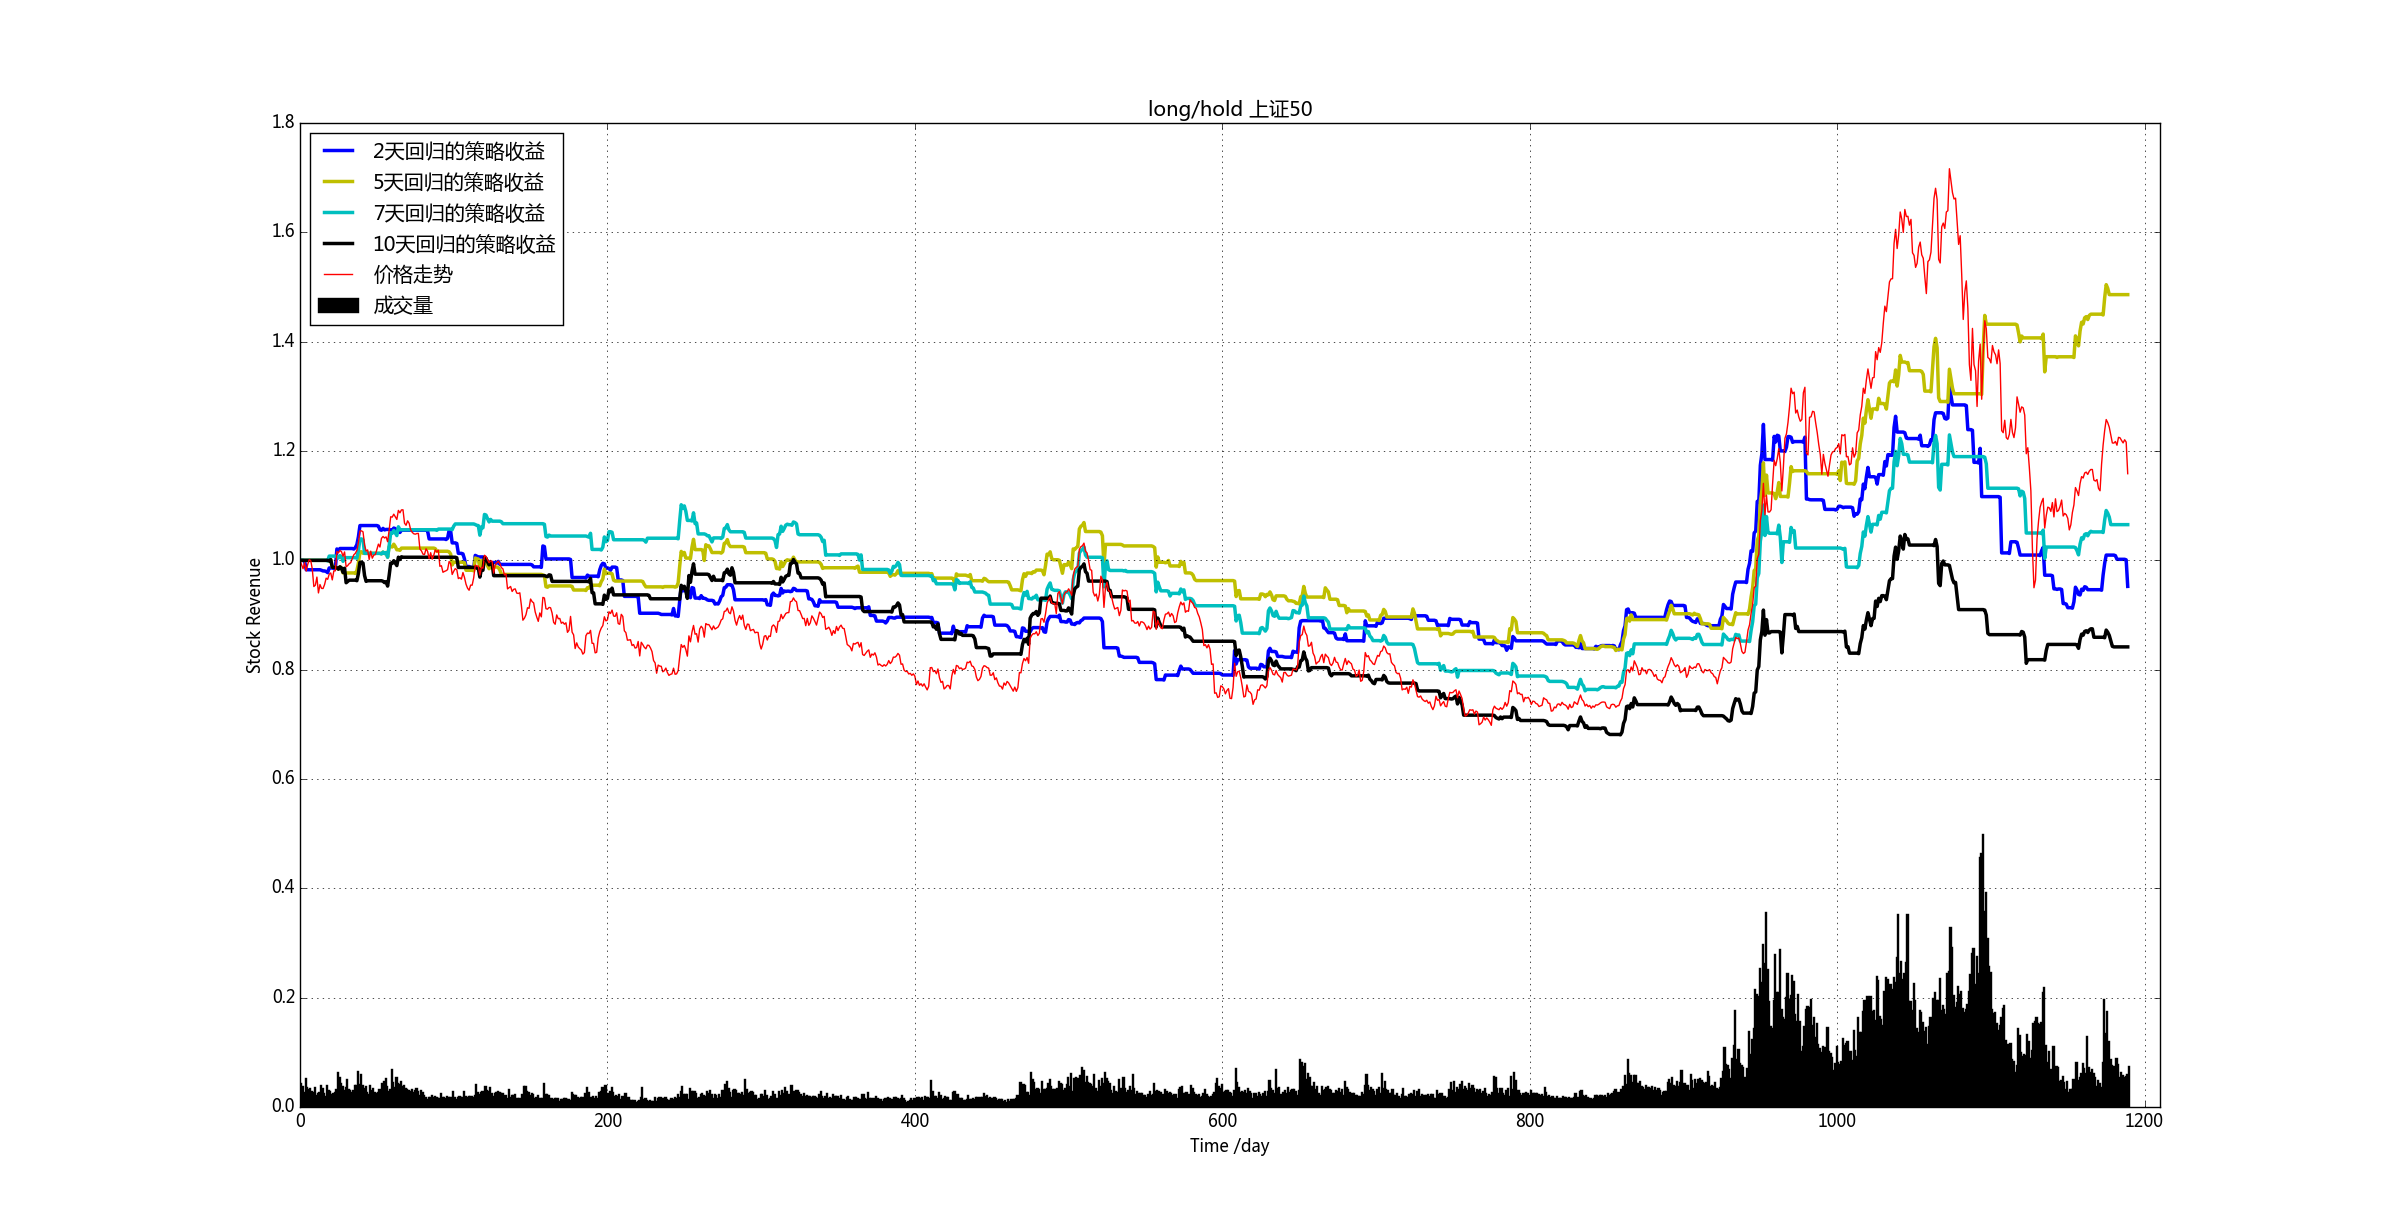
\includegraphics[width=1.0\textwidth]{img_r_2/sz50_1.png}
	\caption{上证50 long/hold}
\end{figure}
\end{enumerate}

\subsubsection{上证综指}

\begin{enumerate}
\item long/short 
\begin{figure}[H]
	\centering
	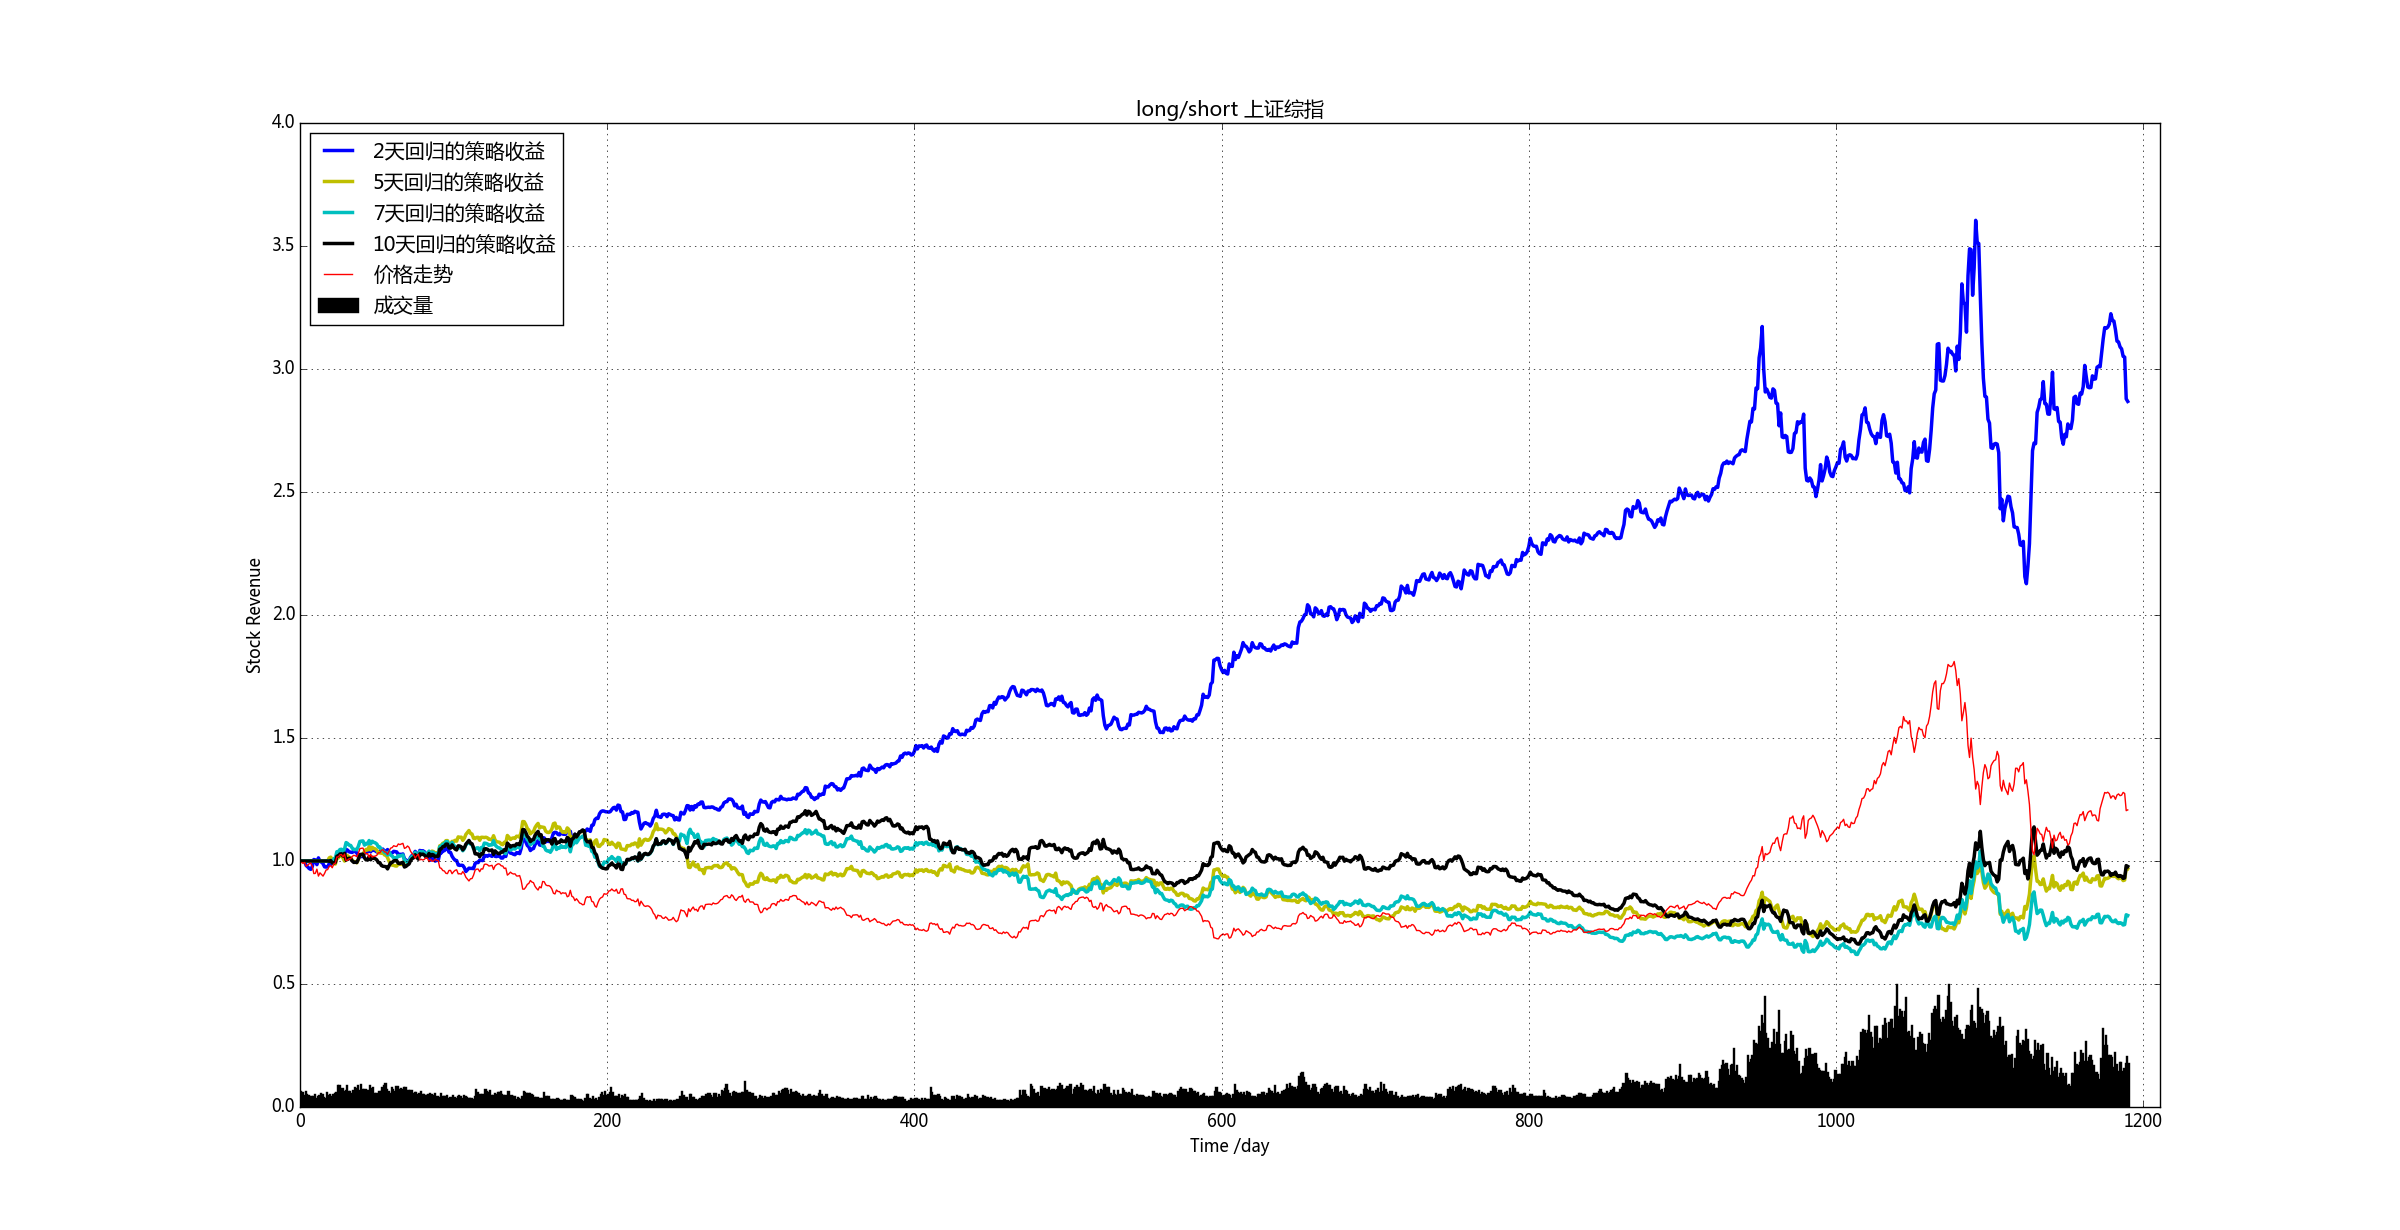
\includegraphics[width=1.0\textwidth]{img_r_2/szzz.png}
	\caption{上证综指 long/short}
\end{figure}
\item long/hold 
\begin{figure}[H]
	\centering
	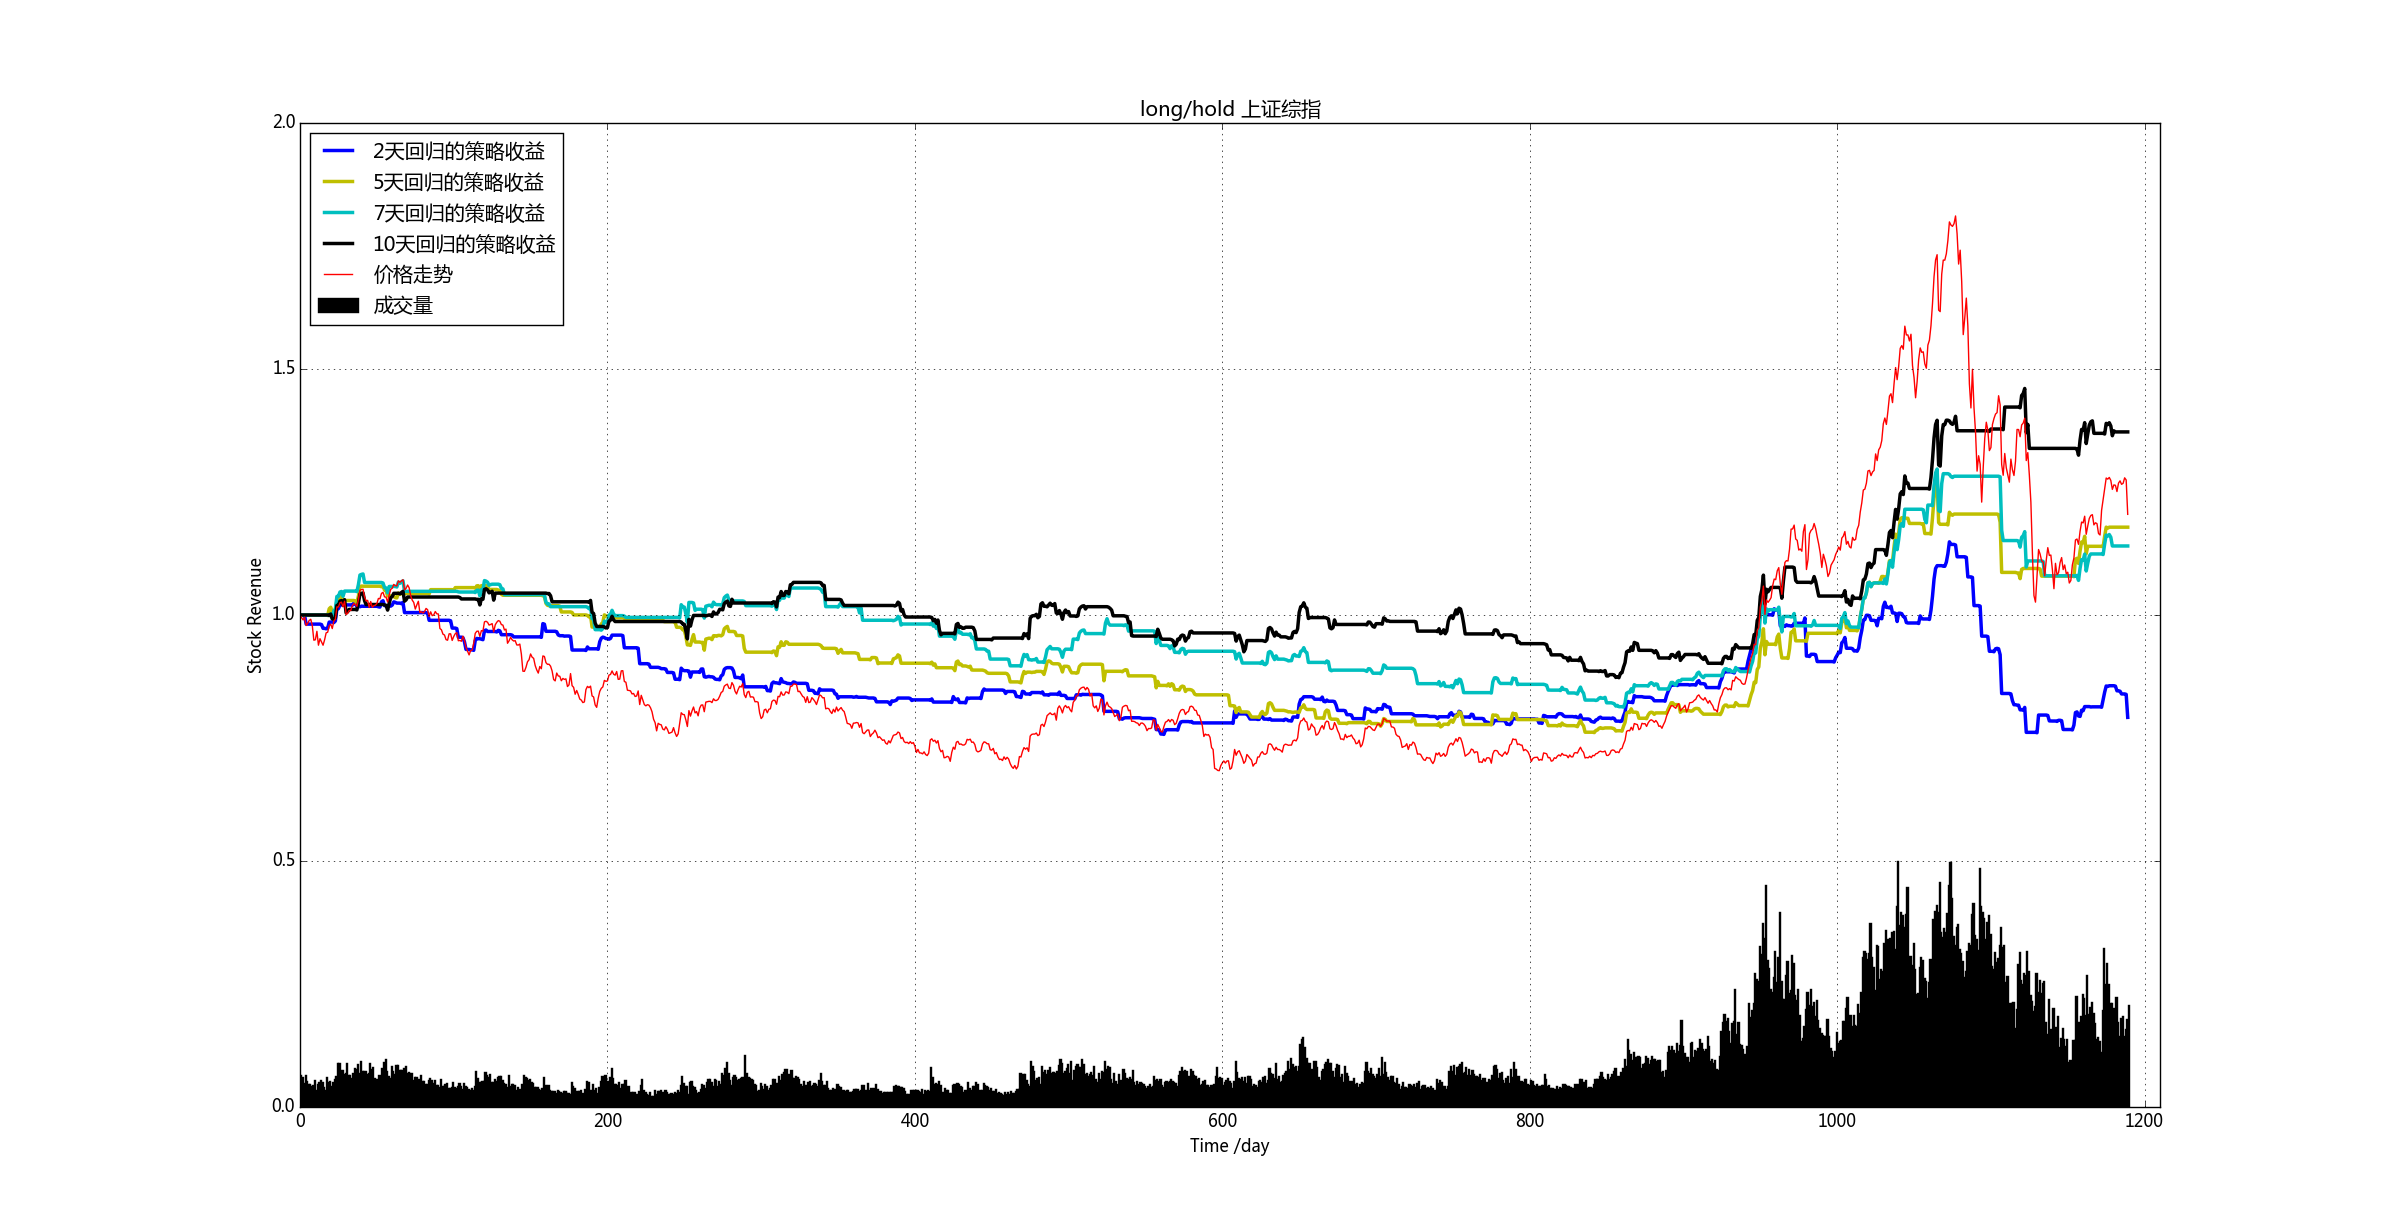
\includegraphics[width=1.0\textwidth]{img_r_2/szzz_1.png}
	\caption{上证综指 long/hold}
\end{figure}
\end{enumerate}

\subsubsection{沪深300}
\begin{enumerate}
\item long/short 
\begin{figure}[H]
	\centering
	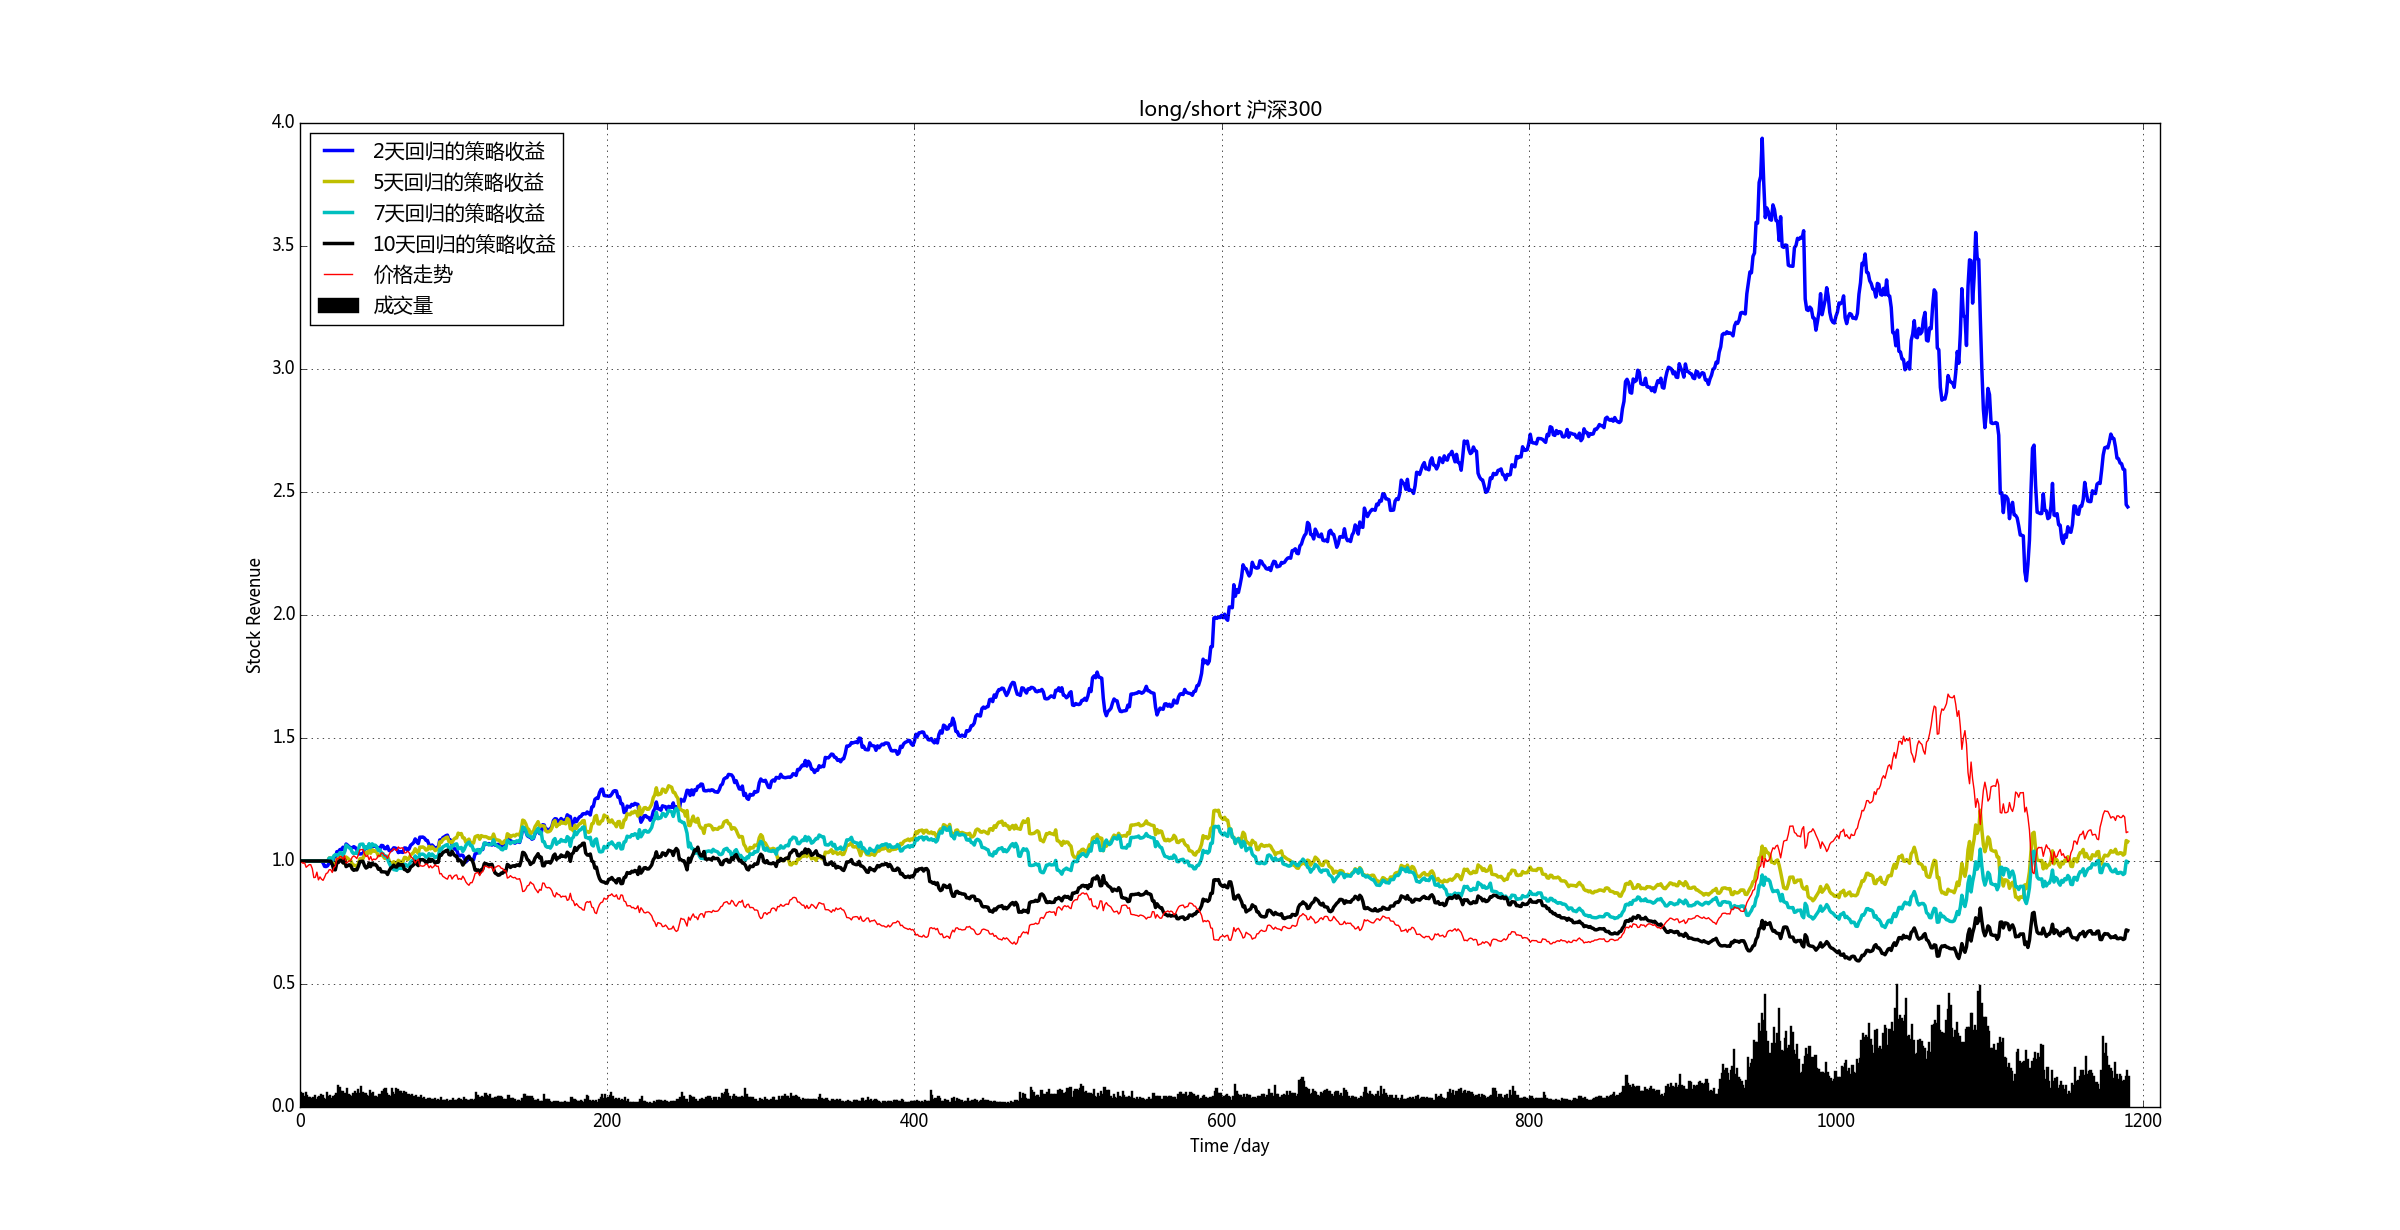
\includegraphics[width=1.0\textwidth]{img_r_2/hs300.png}
	\caption{沪深300 long/short }
\end{figure}
\item long/hold 
\begin{figure}[H]
	\centering
	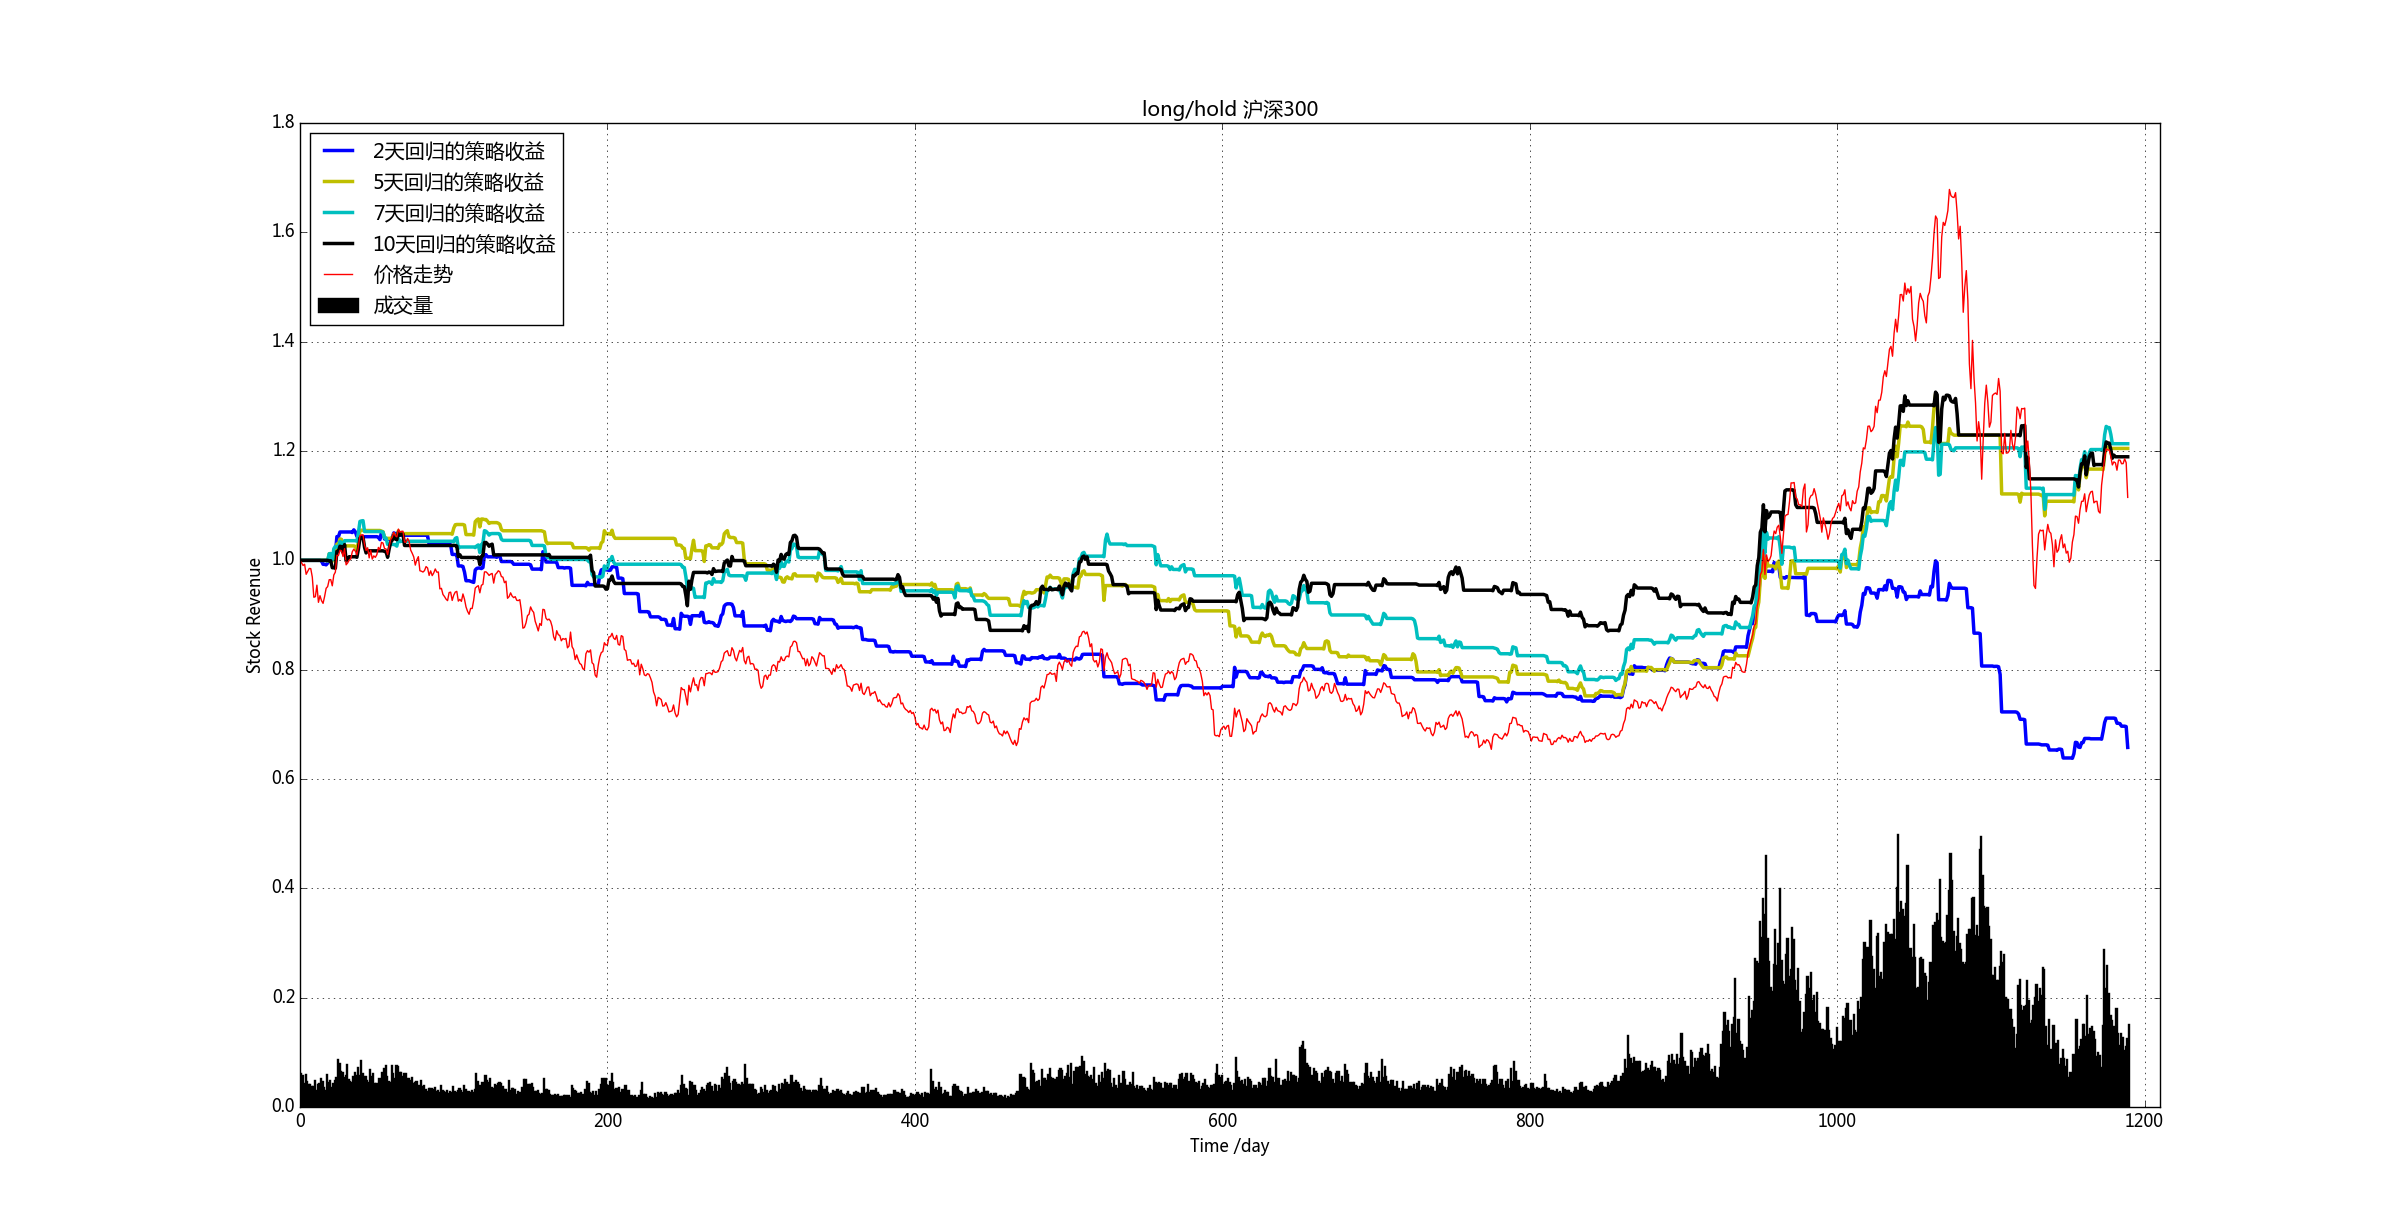
\includegraphics[width=1.0\textwidth]{img_r_2/hs300_1.png}
	\caption{沪深300 long/hold }
\end{figure}
\end{enumerate}

\subsubsection{创业板}
\begin{enumerate}
\item long/short 
\begin{figure}[H]
	\centering
	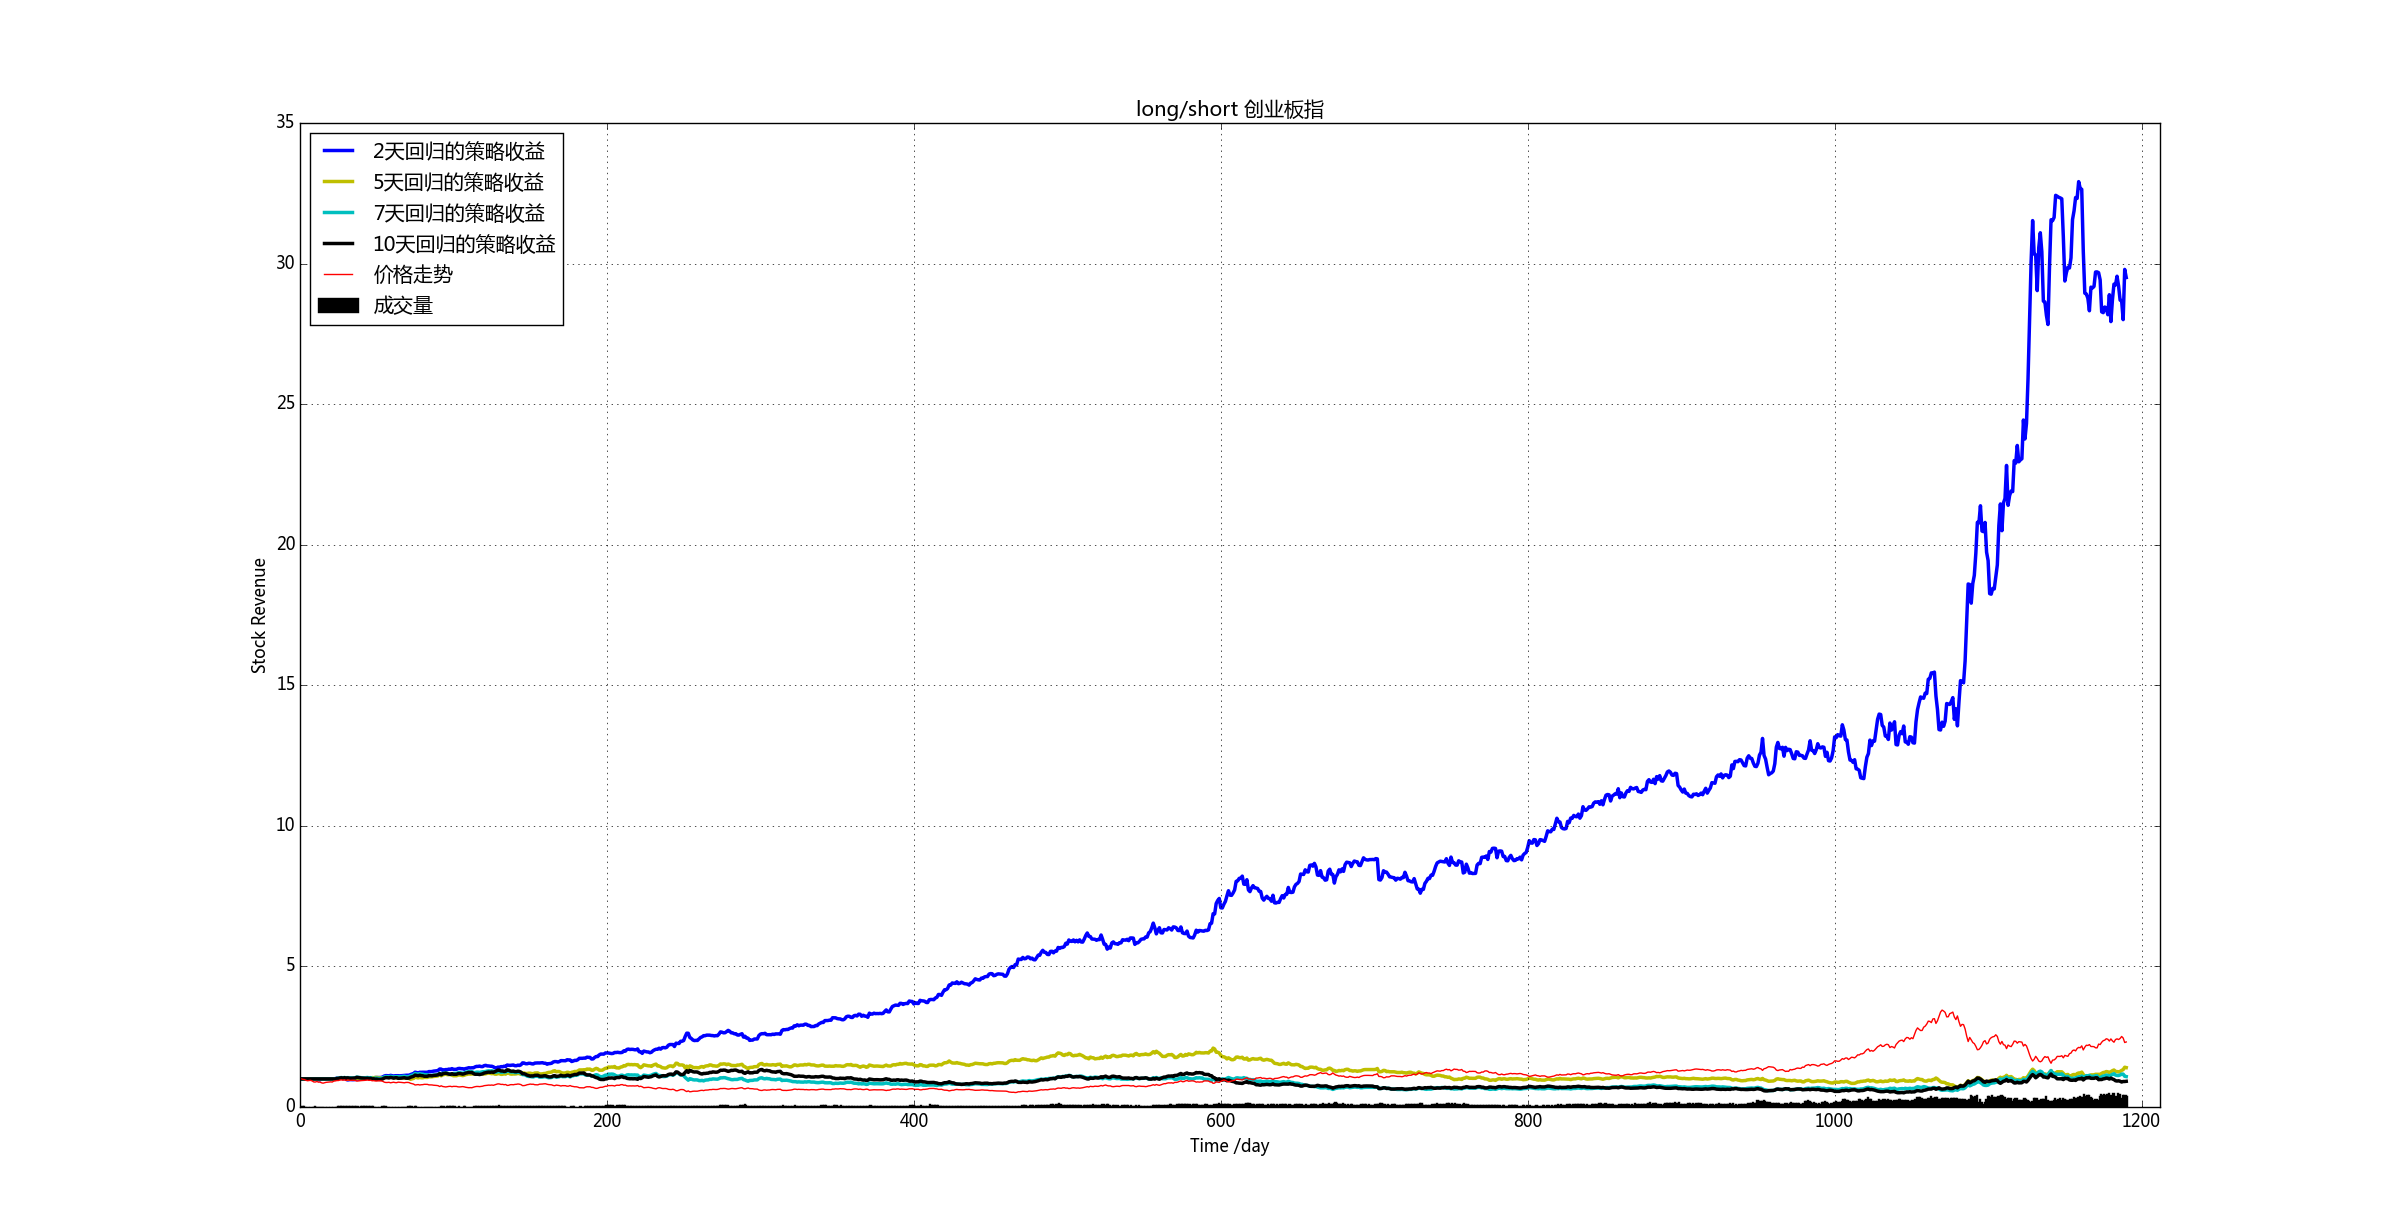
\includegraphics[width=1.0\textwidth]{img_r_1/cyb.png}
	\caption{创业板 long/short}
\end{figure}
\item long/hold 
\begin{figure}[H]
	\centering
	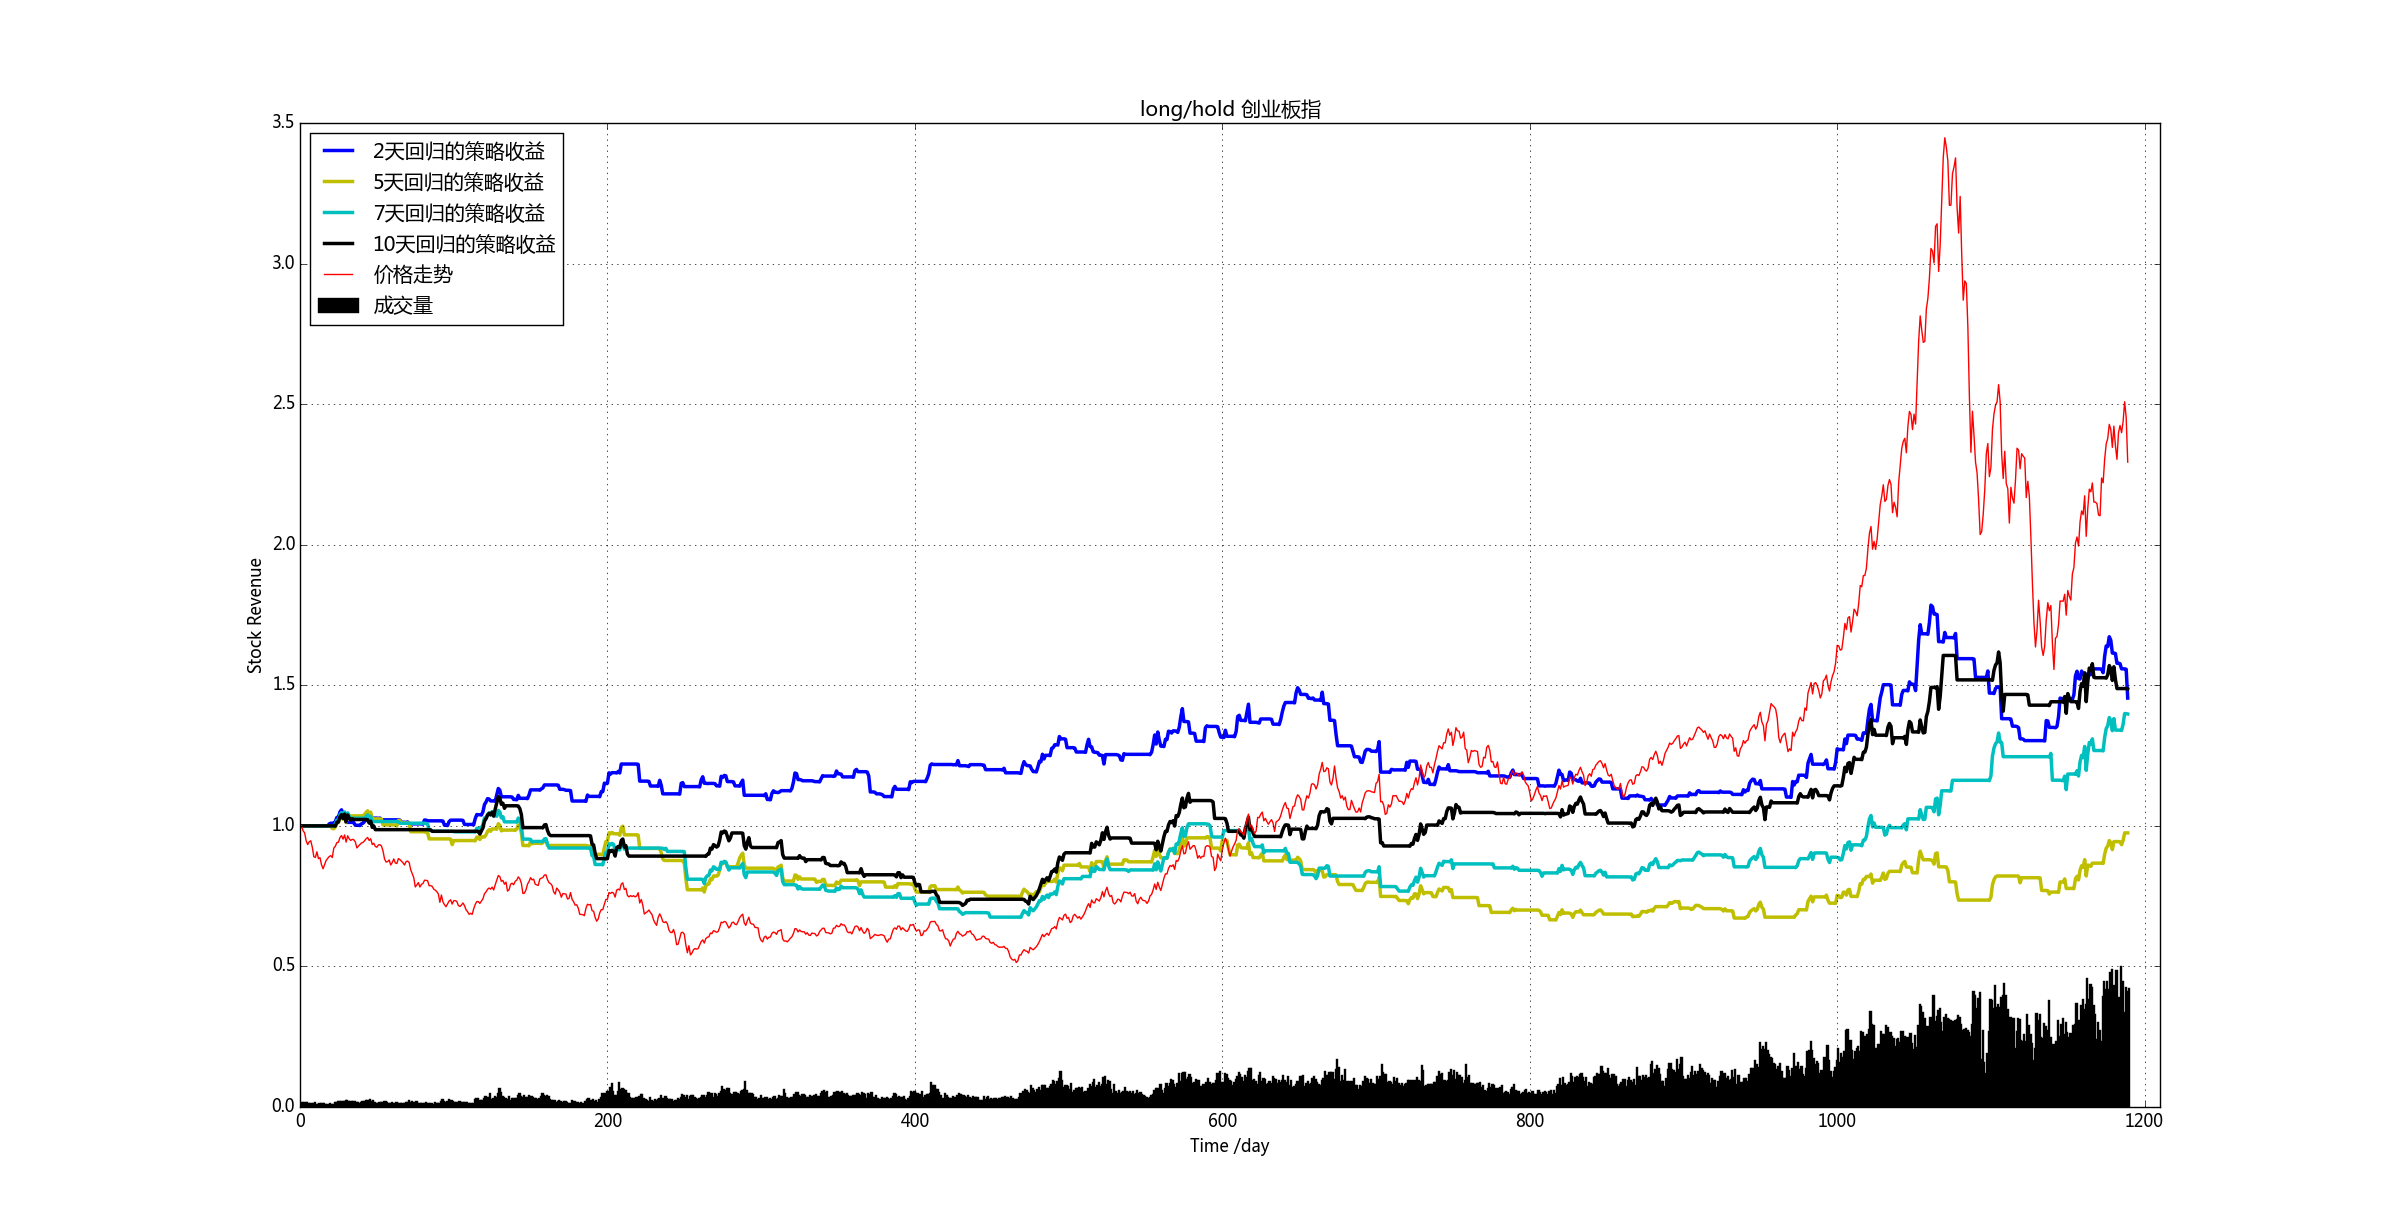
\includegraphics[width=1.0\textwidth]{img_r_2/cyb_1.png}
	\caption{创业板 long/hold }
\end{figure}
\end{enumerate}

\subsubsection{中证500}
\begin{enumerate}
\item long/short 
\begin{figure}[H]
	\centering
	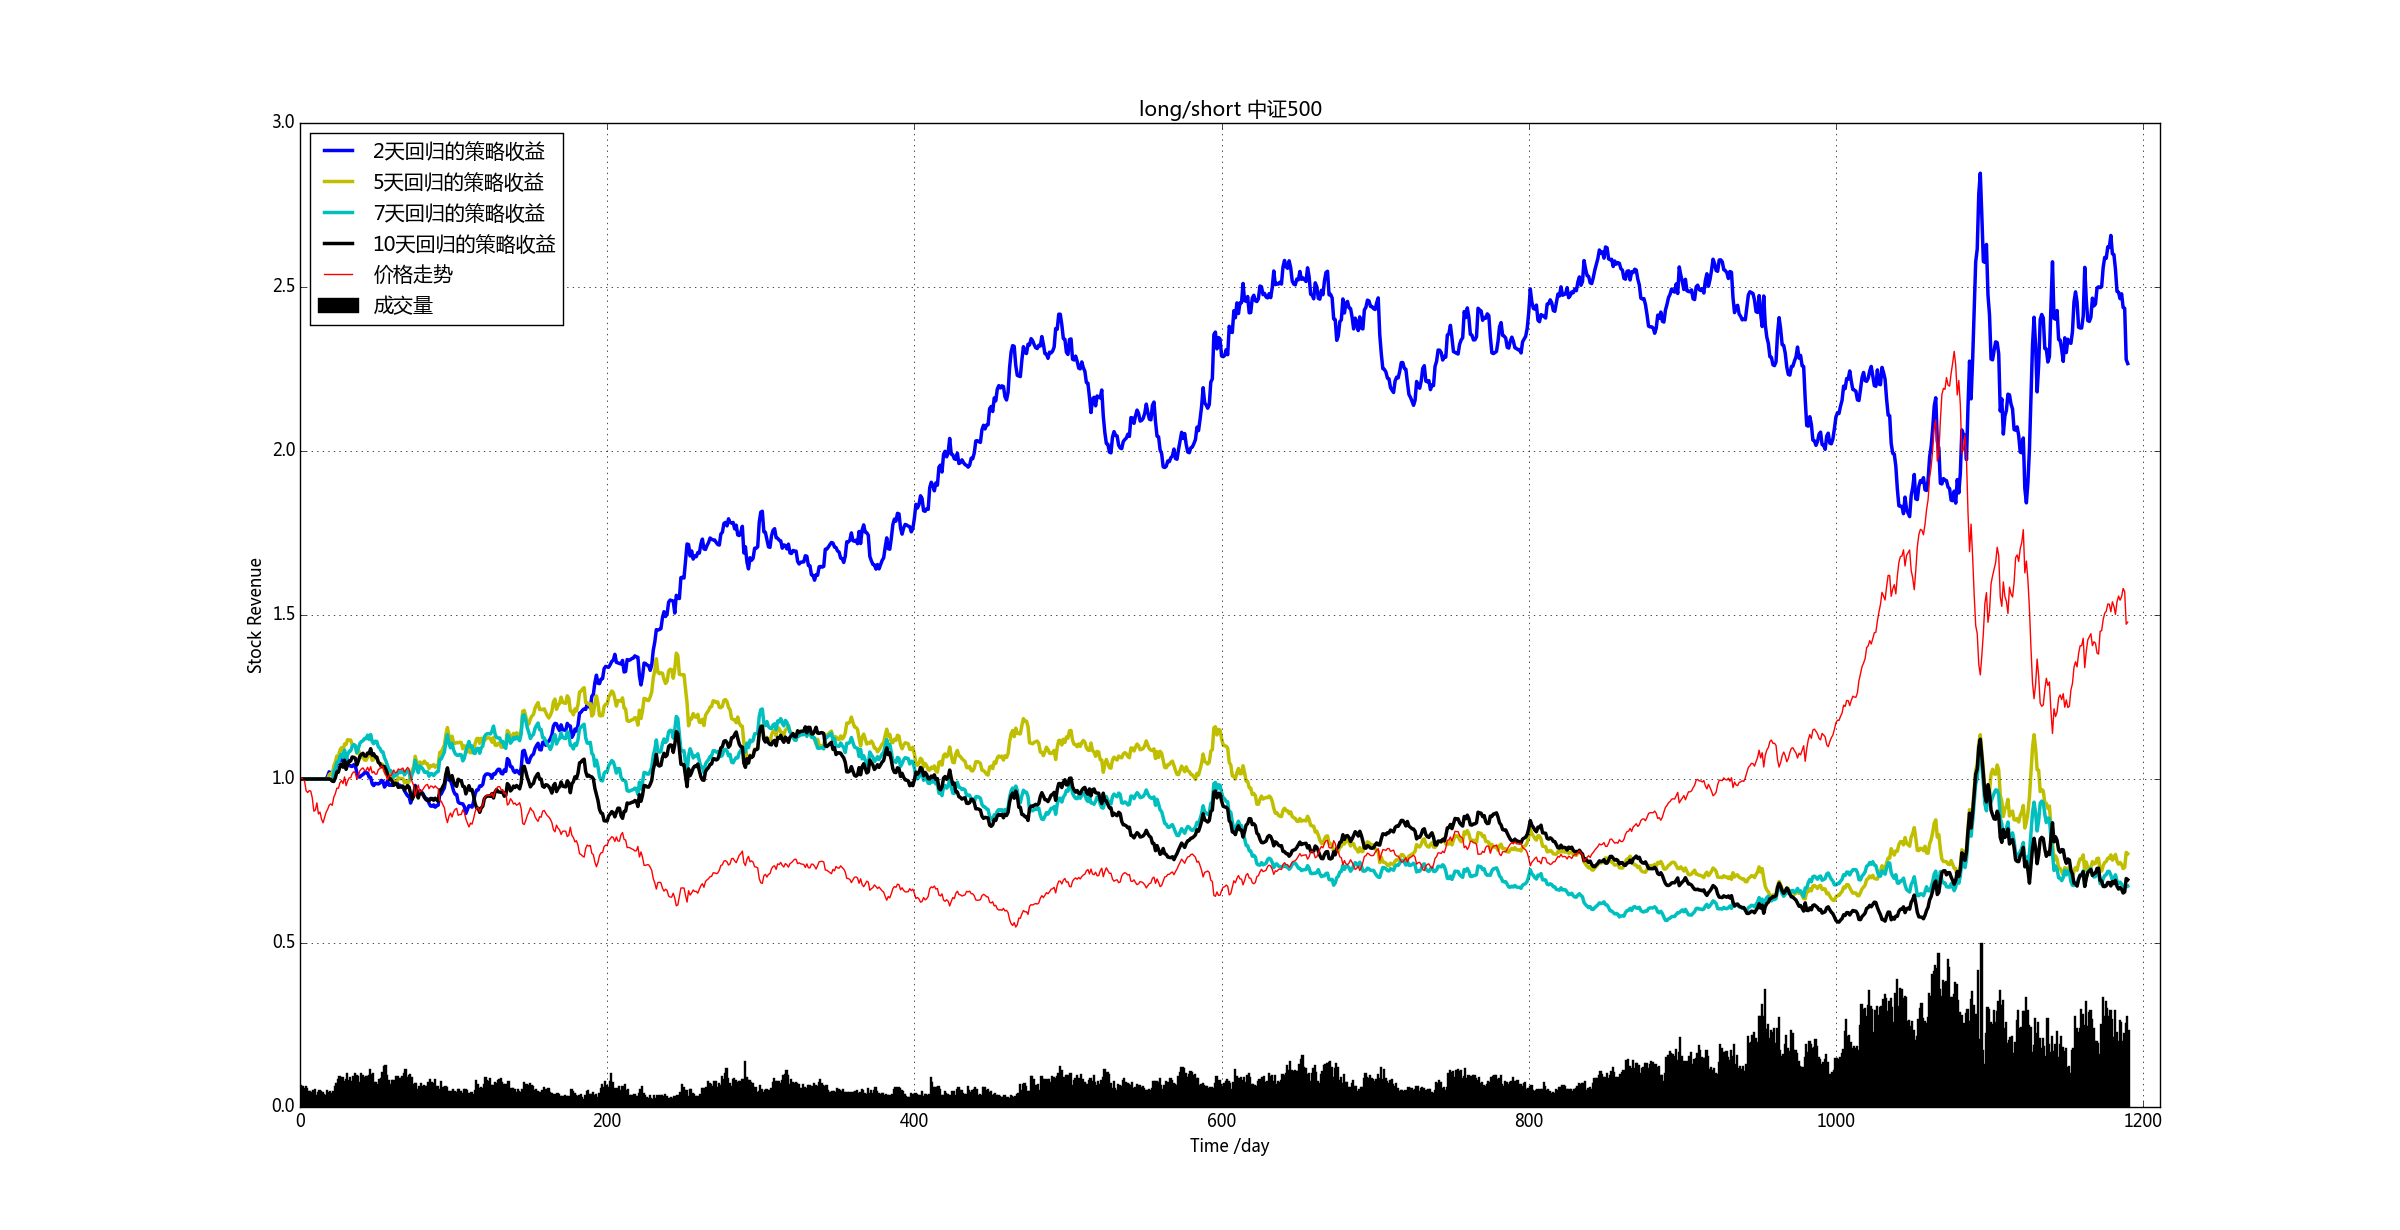
\includegraphics[width=1.0\textwidth]{img_r_2/zz500.png}
	\caption{中证500 long/short }
\end{figure}
\item long/hold 
\begin{figure}[H]
	\centering
	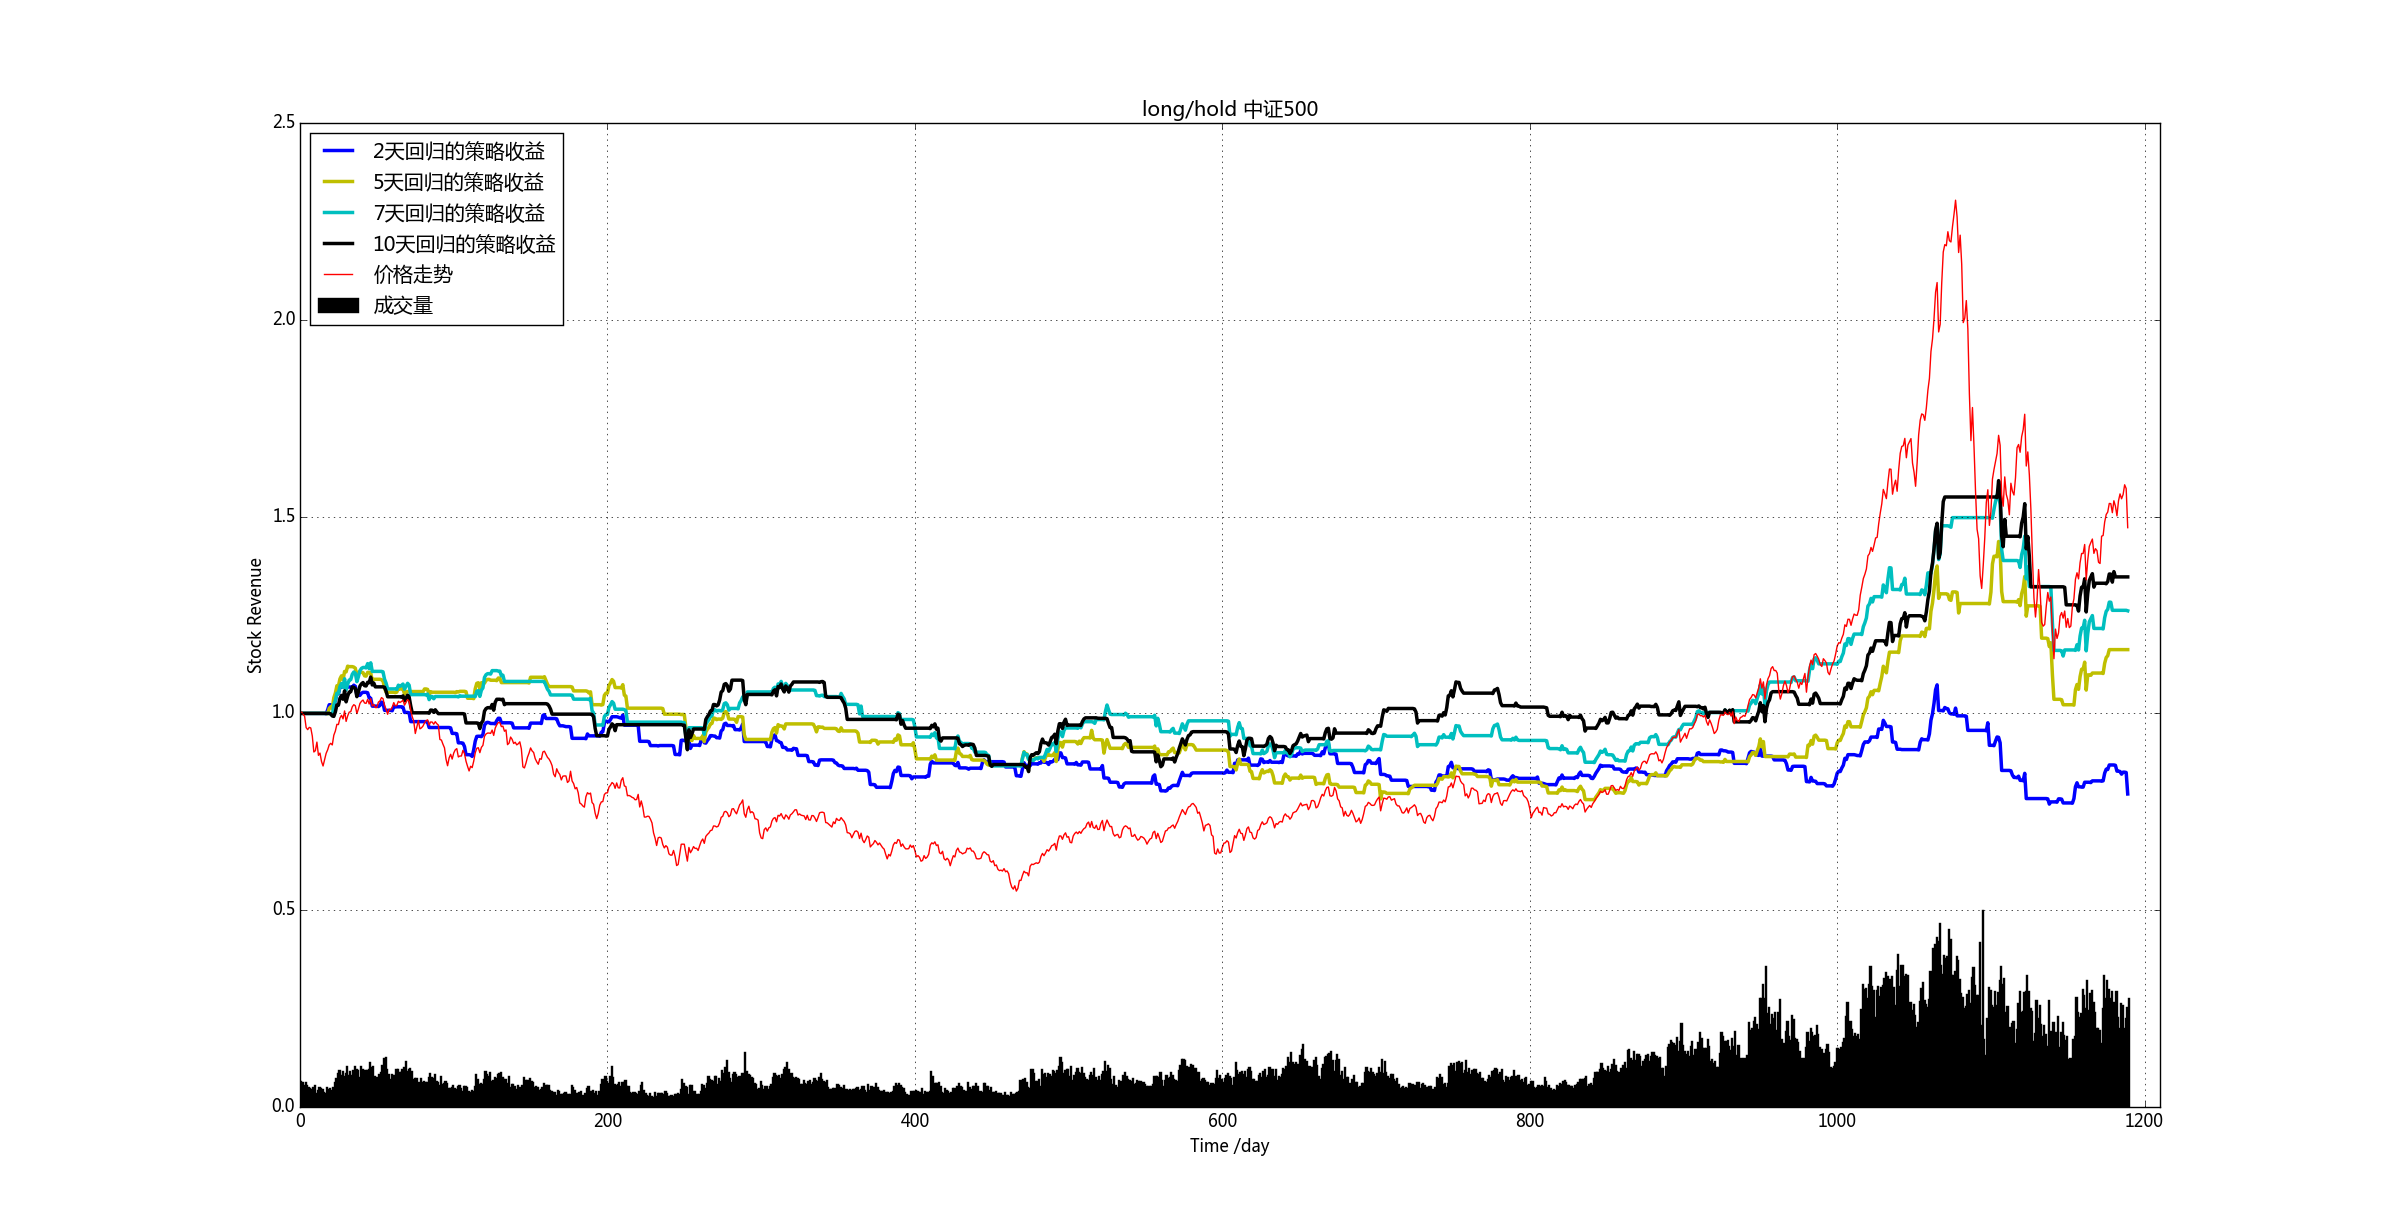
\includegraphics[width=1.0\textwidth]{img_r_2/zz500_1.png}
	\caption{中证500 long/hold}
\end{figure}
\end{enumerate}

\subsection{价格和成交量5日MA}
\subsubsection{上证50}

\begin{enumerate}
\item long/short 
\begin{figure}[H]
	\centering
	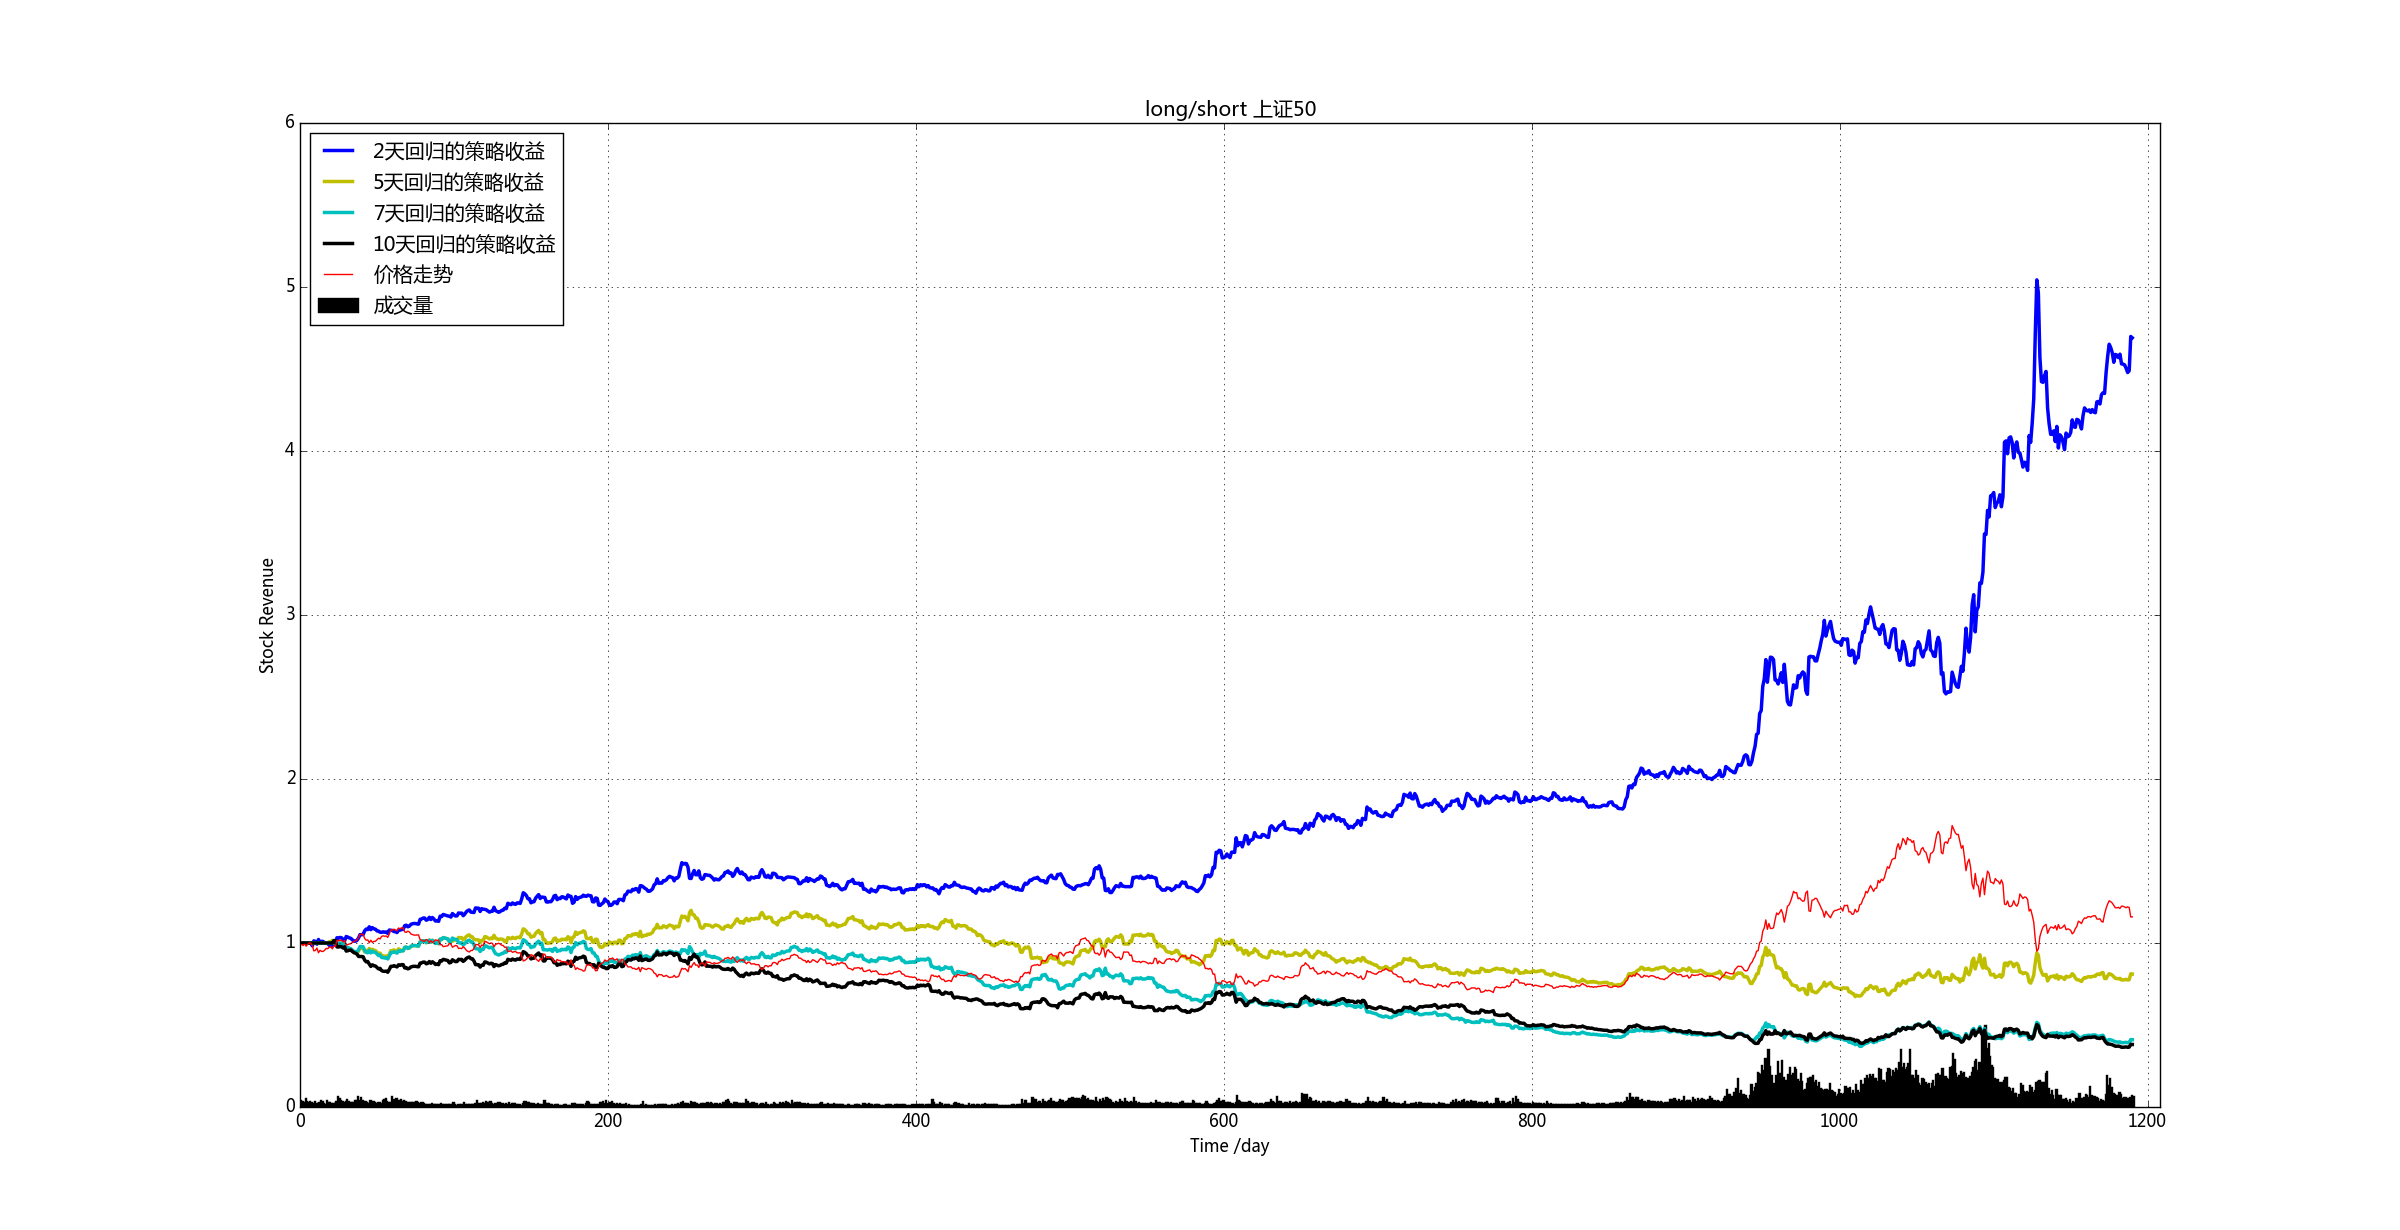
\includegraphics[width=1.0\textwidth]{img_r_5/sz50.png}
	\caption{上证50 long/short}
\end{figure}

\item long/hold 
\begin{figure}[H]
	\centering
	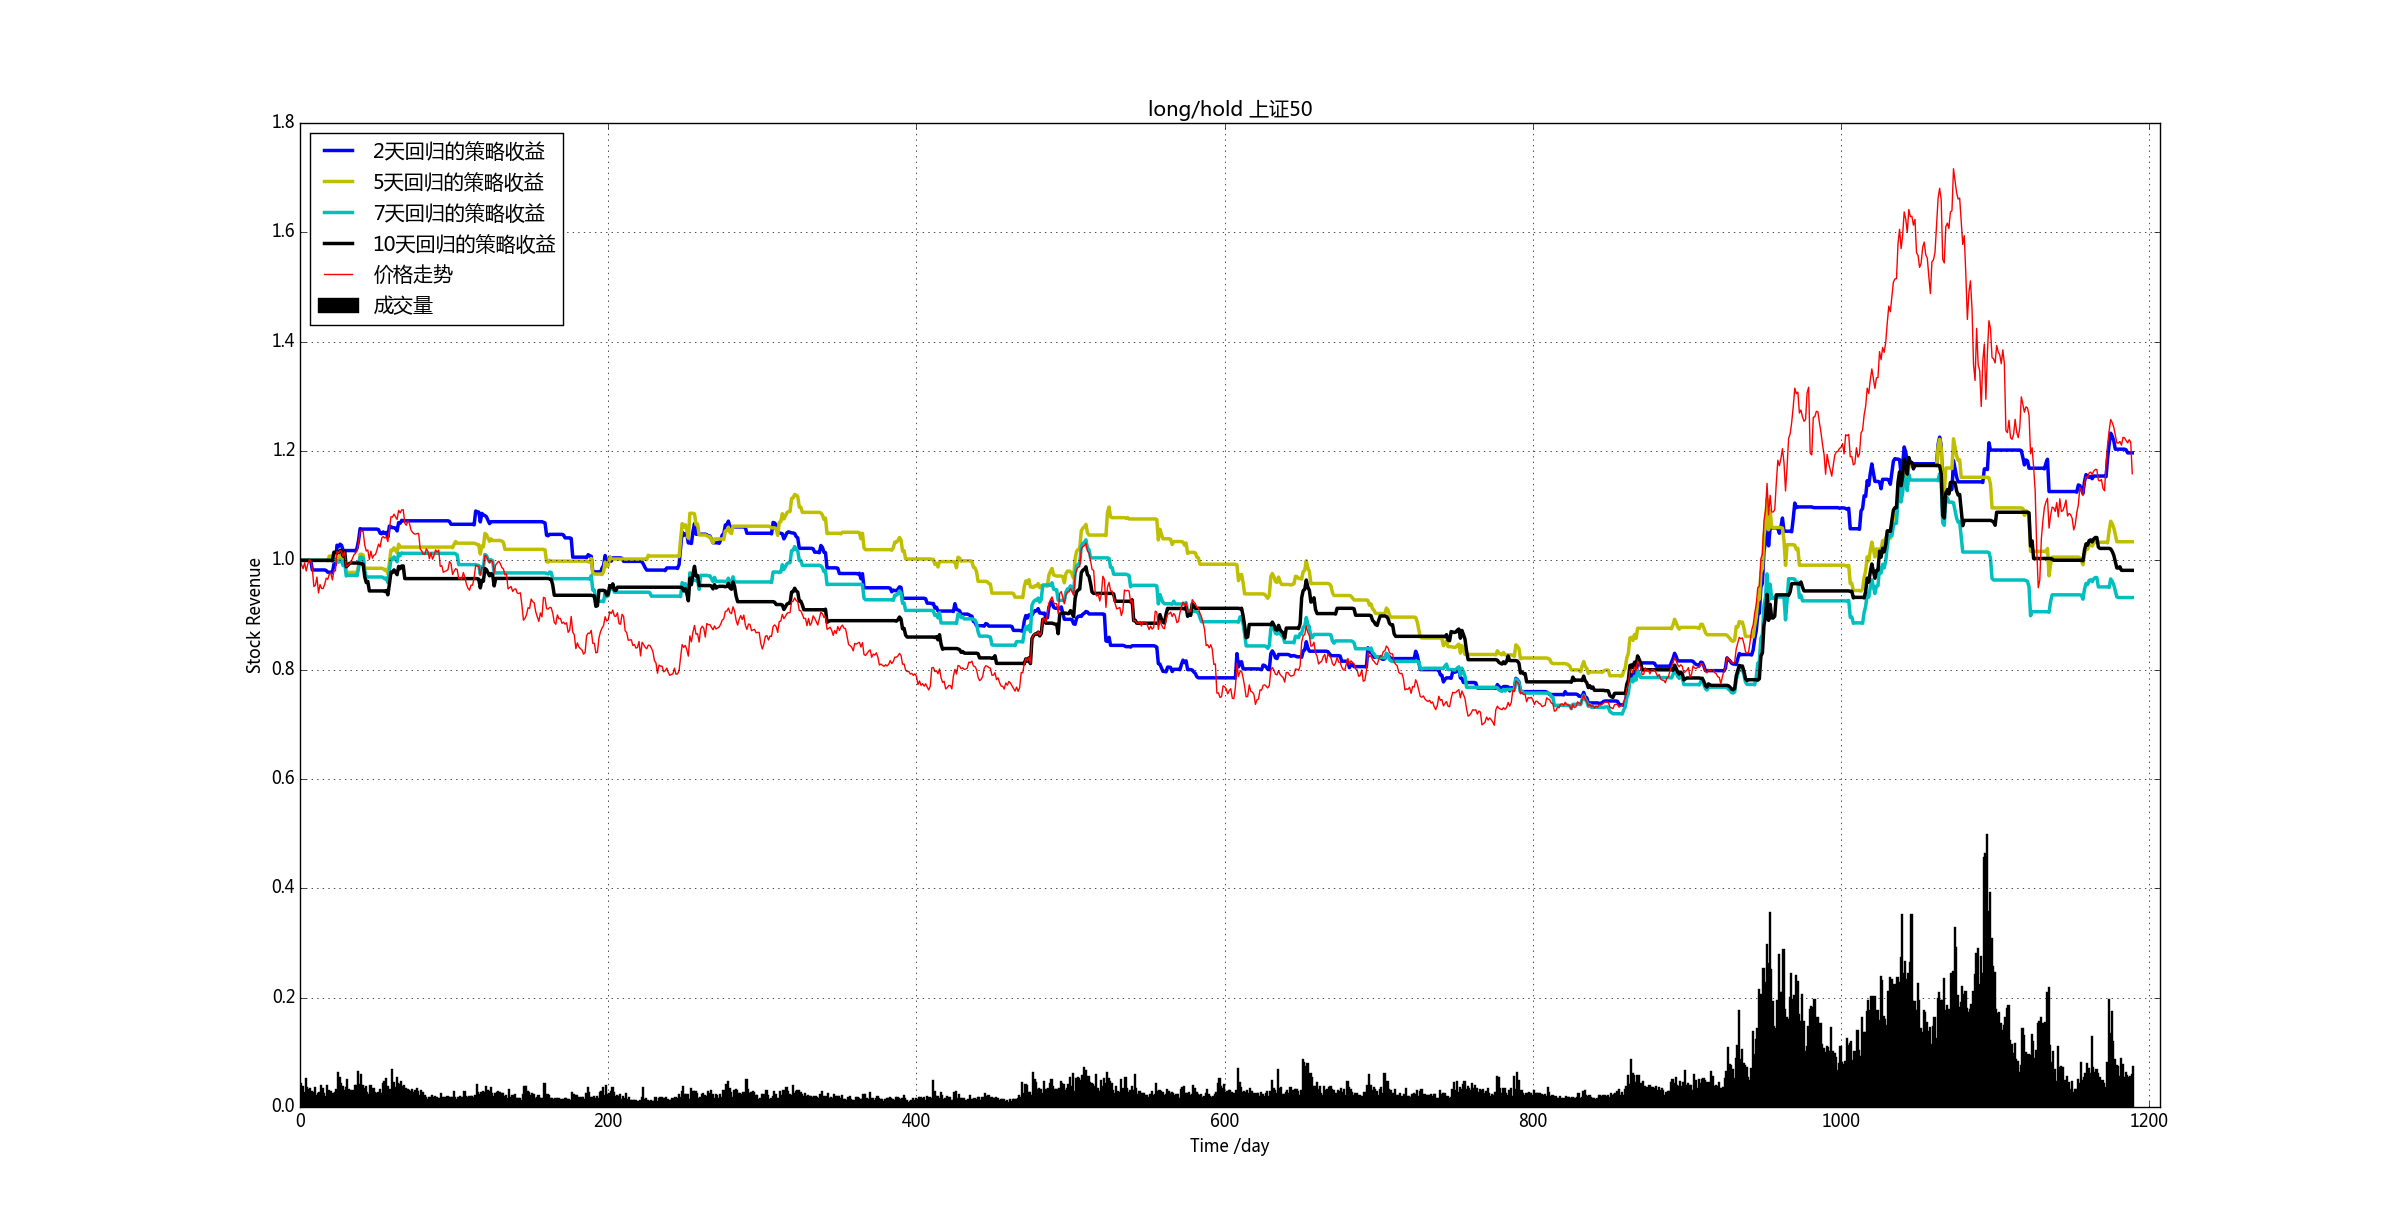
\includegraphics[width=1.0\textwidth]{img_r_5/sz50_1.png}
	\caption{上证50 long/hold}
\end{figure}
\end{enumerate}

\subsubsection{上证综指}

\begin{enumerate}
\item long/short 
\begin{figure}[H]
	\centering
	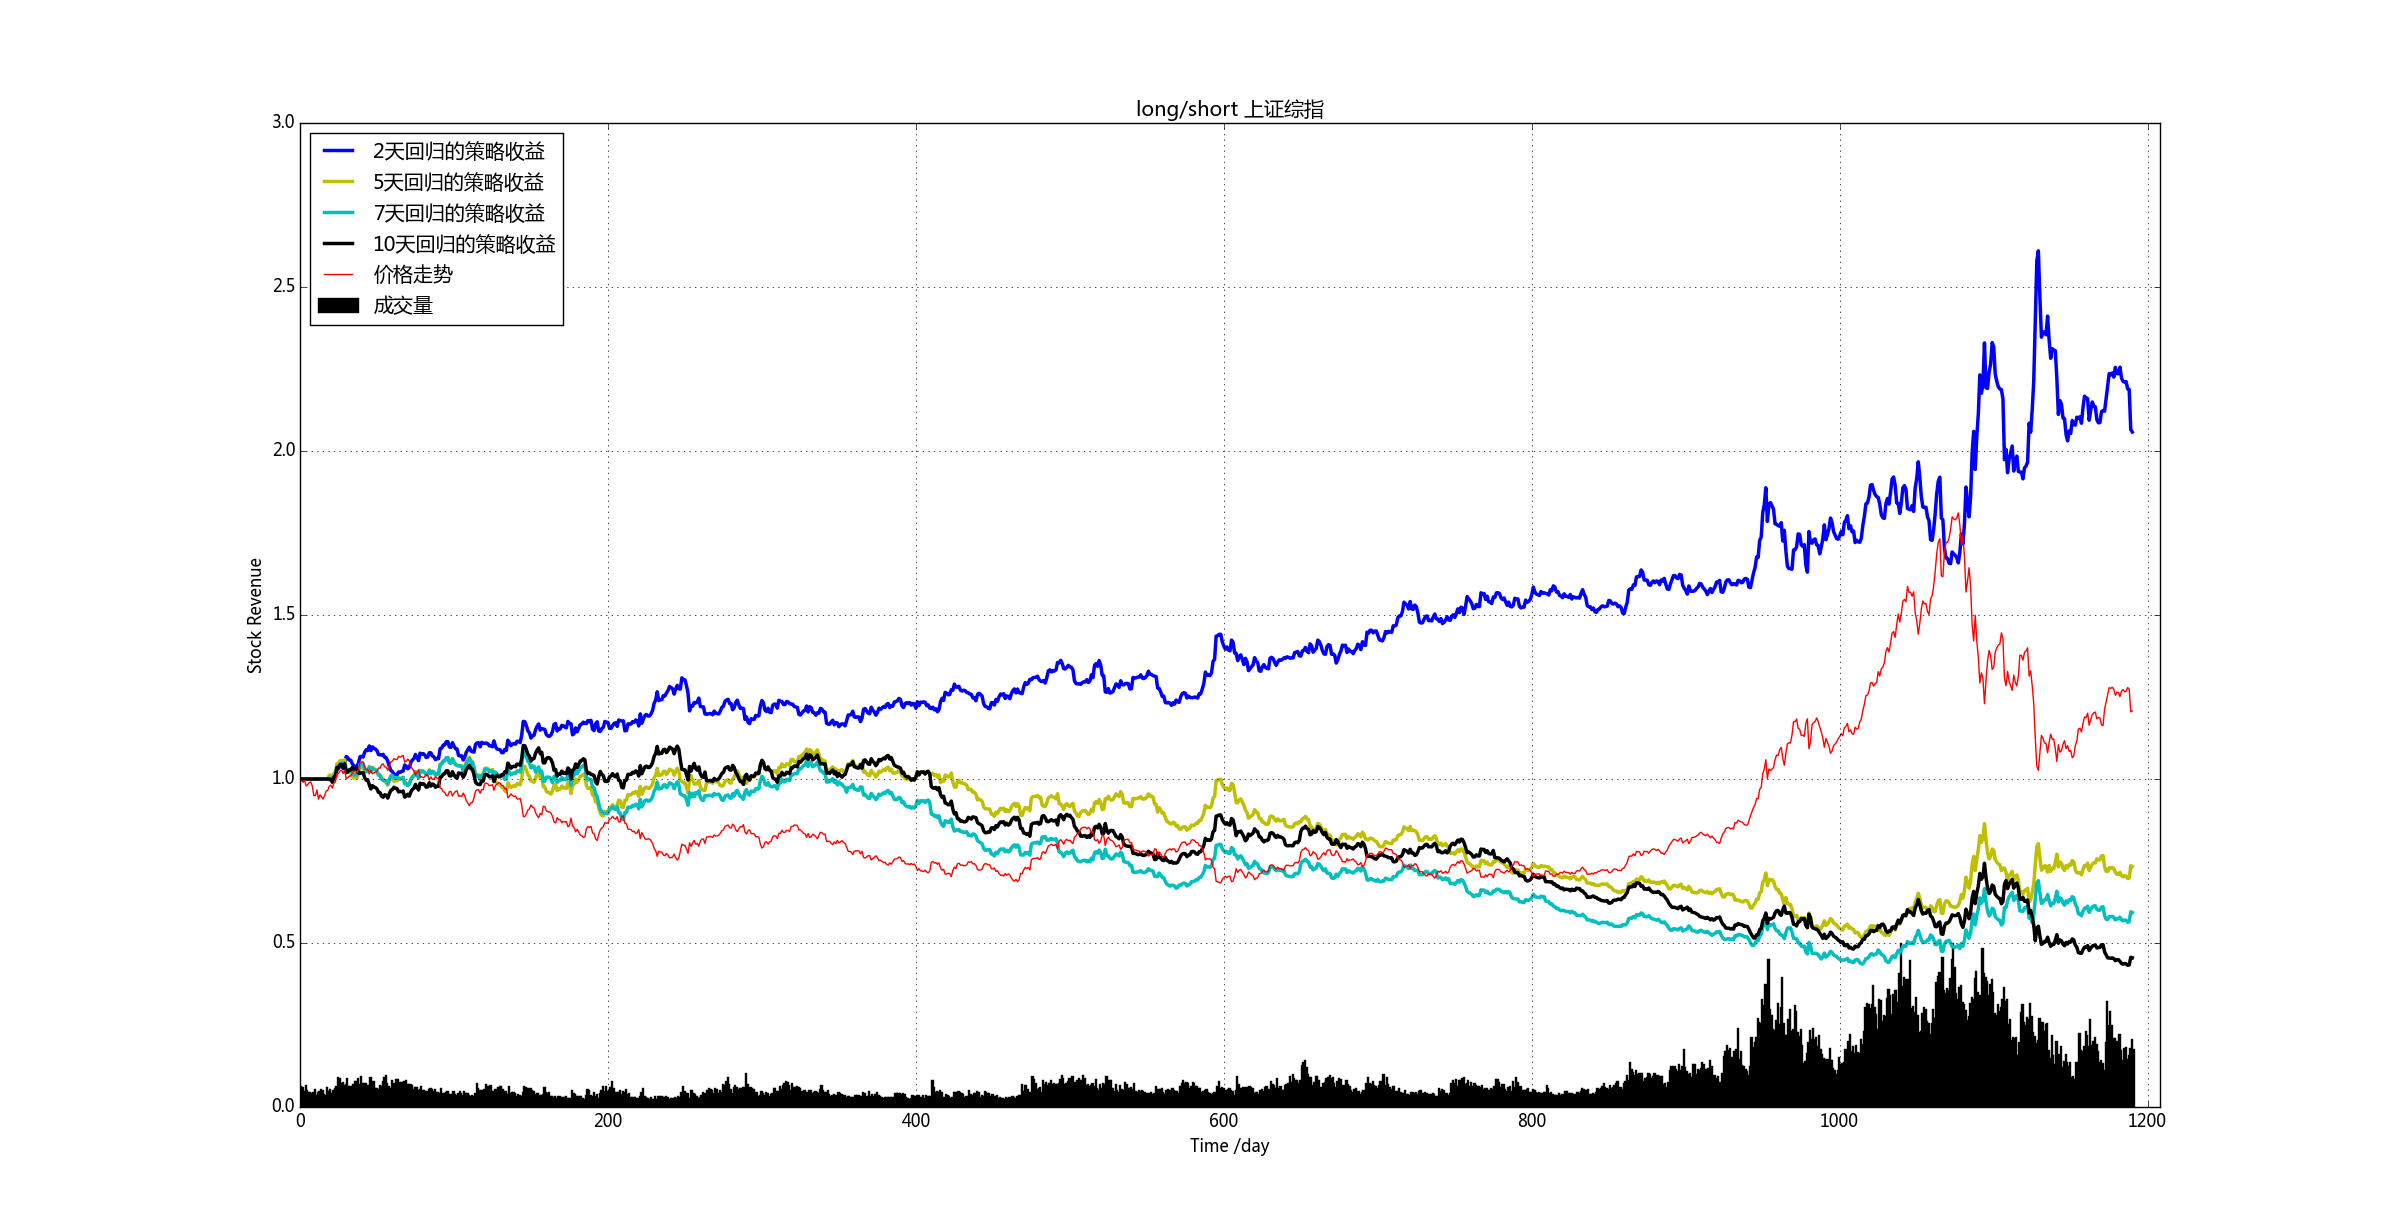
\includegraphics[width=1.0\textwidth]{img_r_5/szzz.png}
	\caption{上证综指 long/short}
\end{figure}
\item long/hold 
\begin{figure}[H]
	\centering
	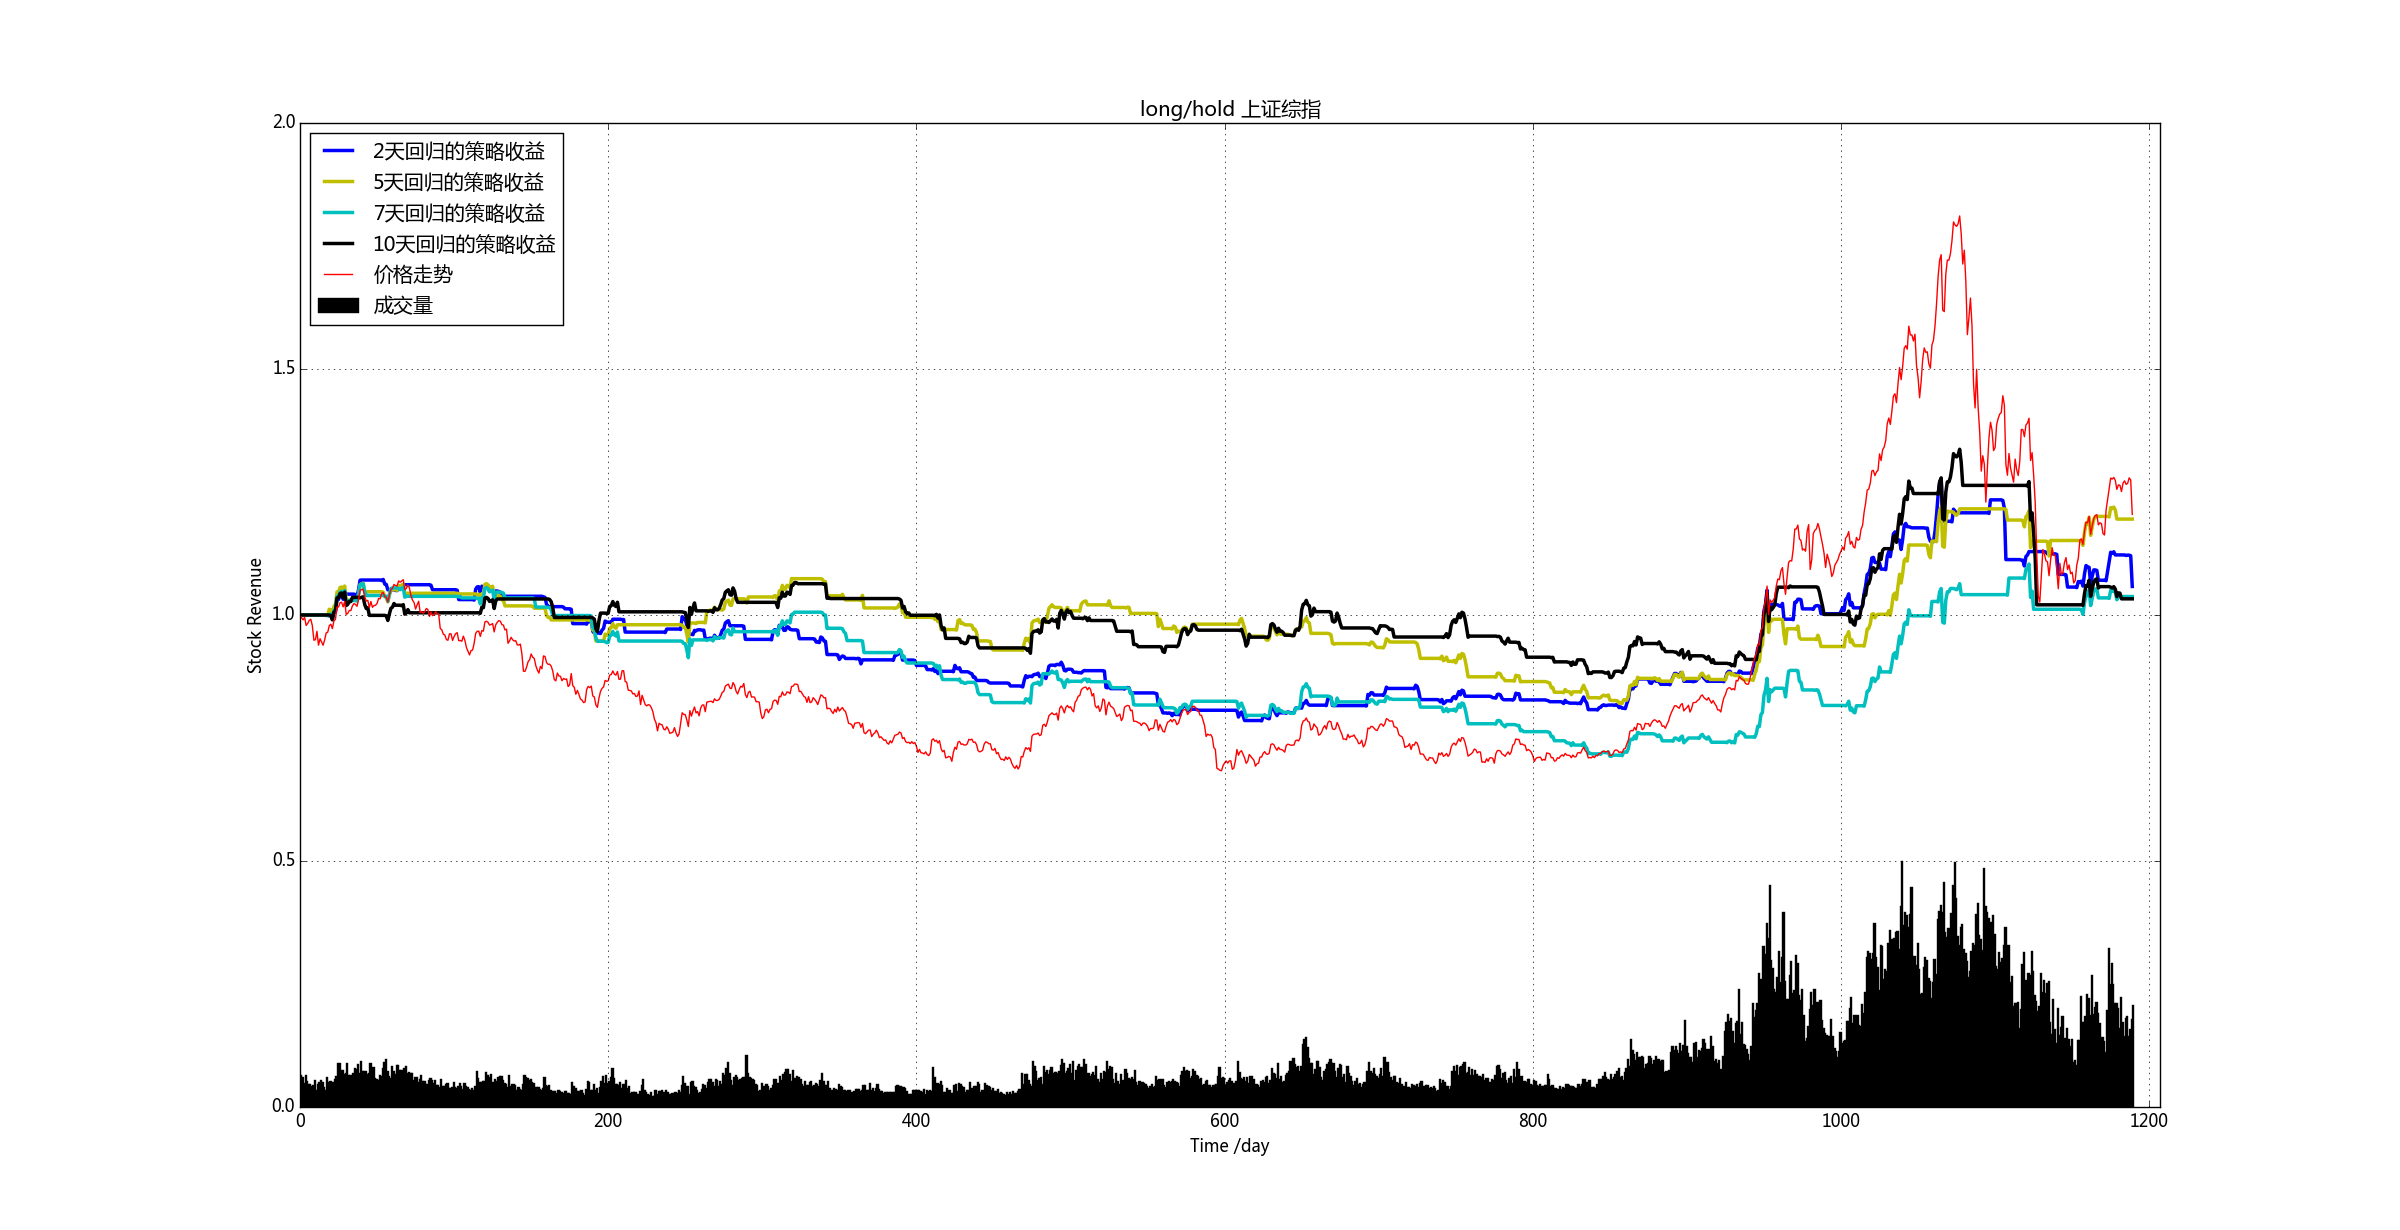
\includegraphics[width=1.0\textwidth]{img_r_5/szzz_1.png}
	\caption{上证综指 long/hold}
\end{figure}
\end{enumerate}

\subsubsection{沪深300}
\begin{enumerate}
\item long/short 
\begin{figure}[H]
	\centering
	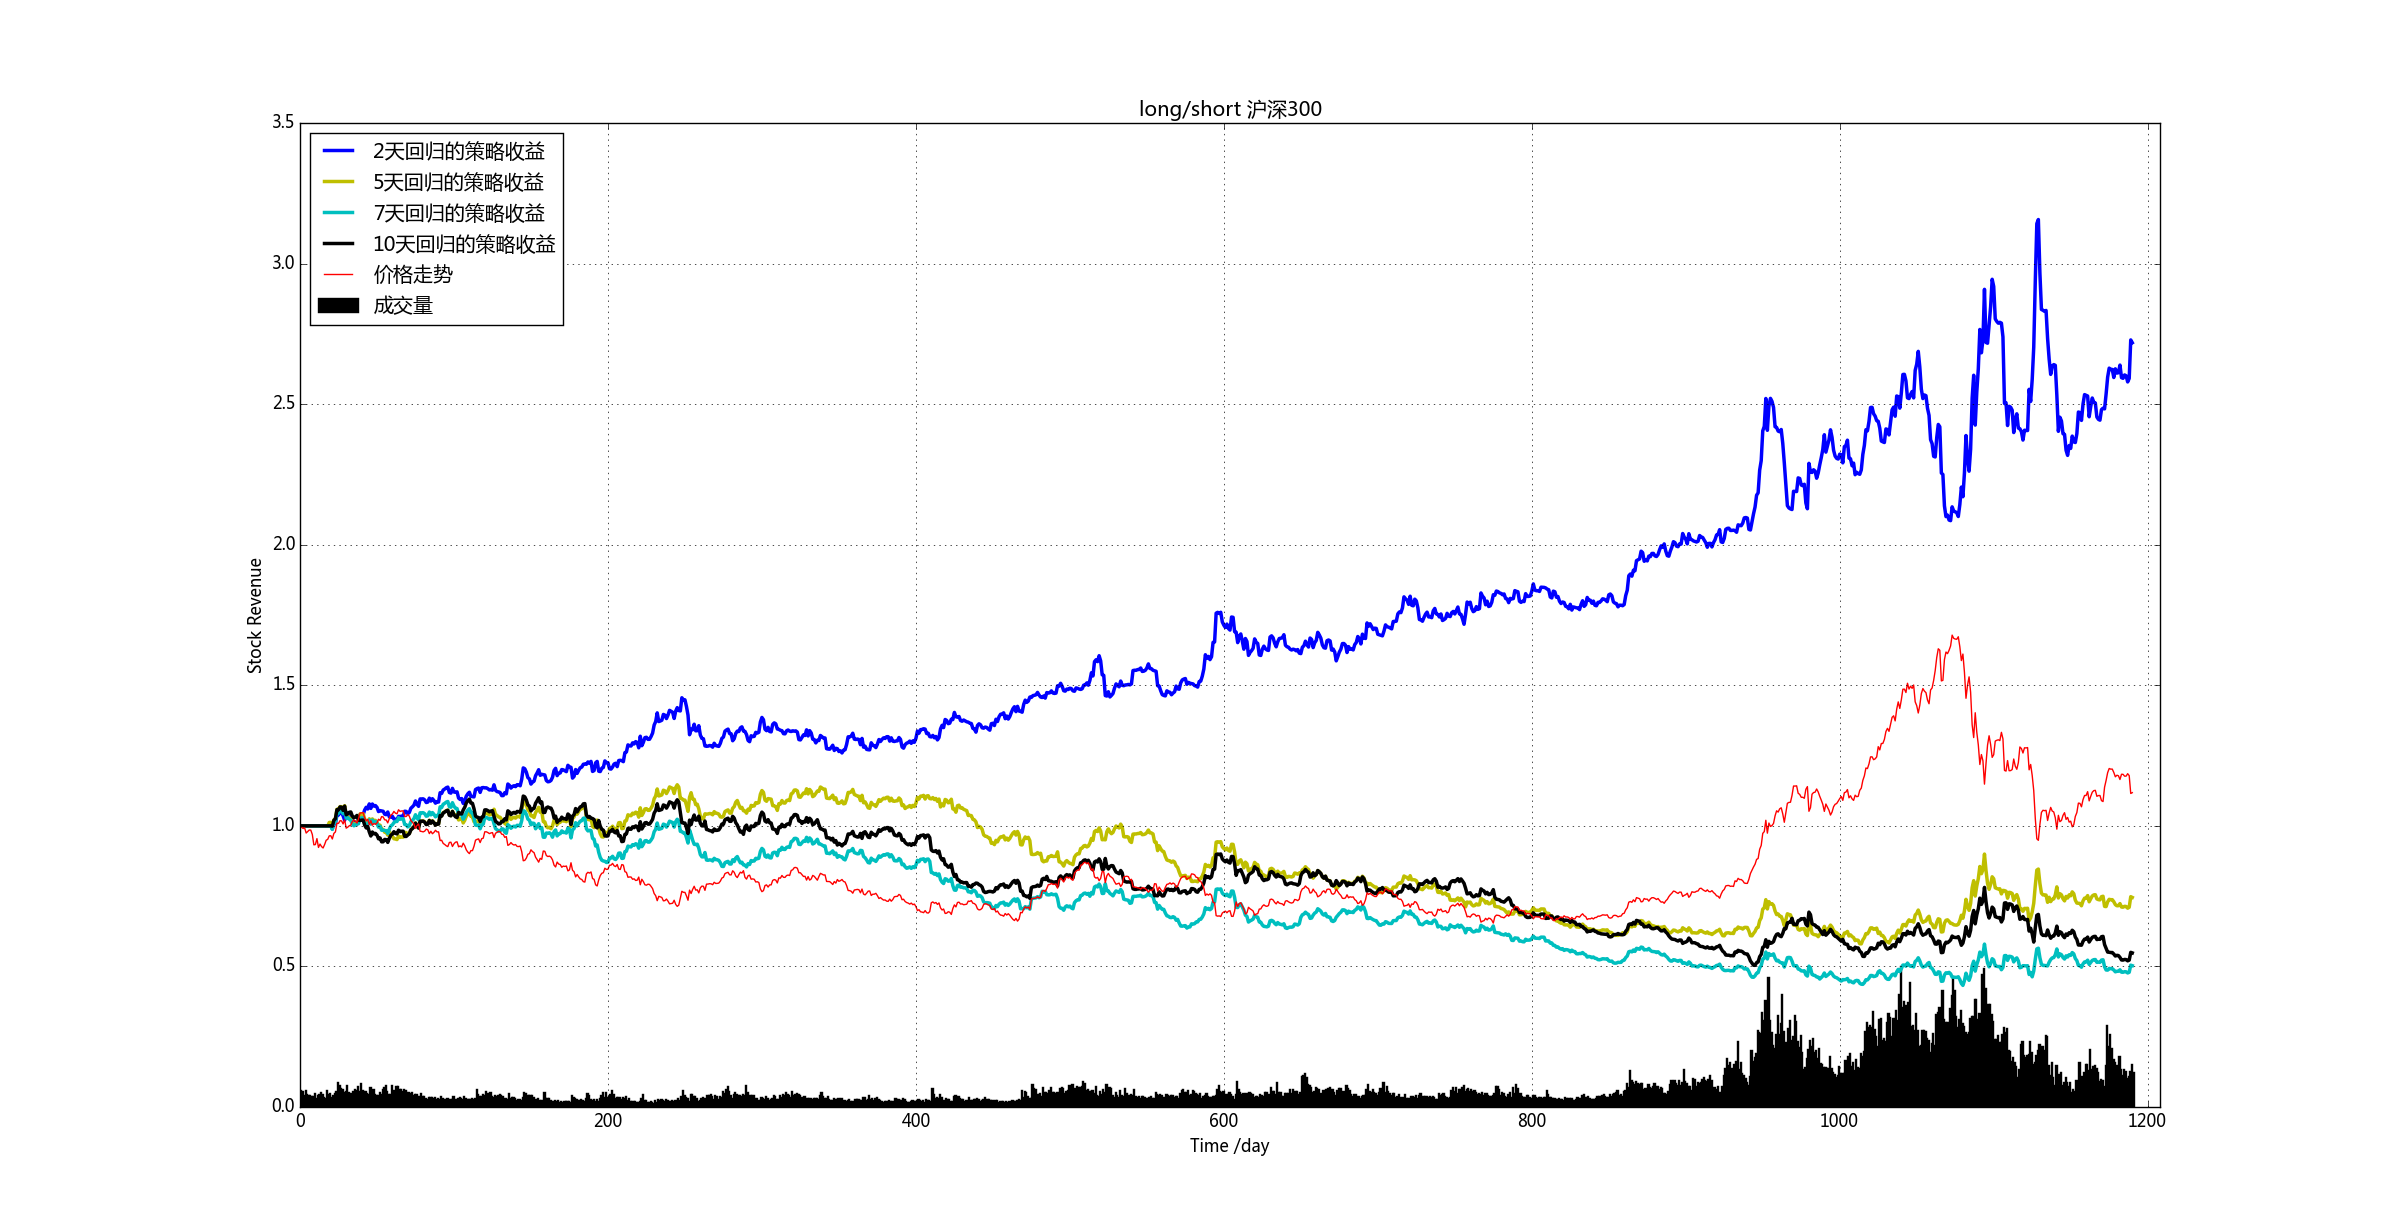
\includegraphics[width=1.0\textwidth]{img_r_5/hs300.png}
	\caption{沪深300 long/short }
\end{figure}
\item long/hold 
\begin{figure}[H]
	\centering
	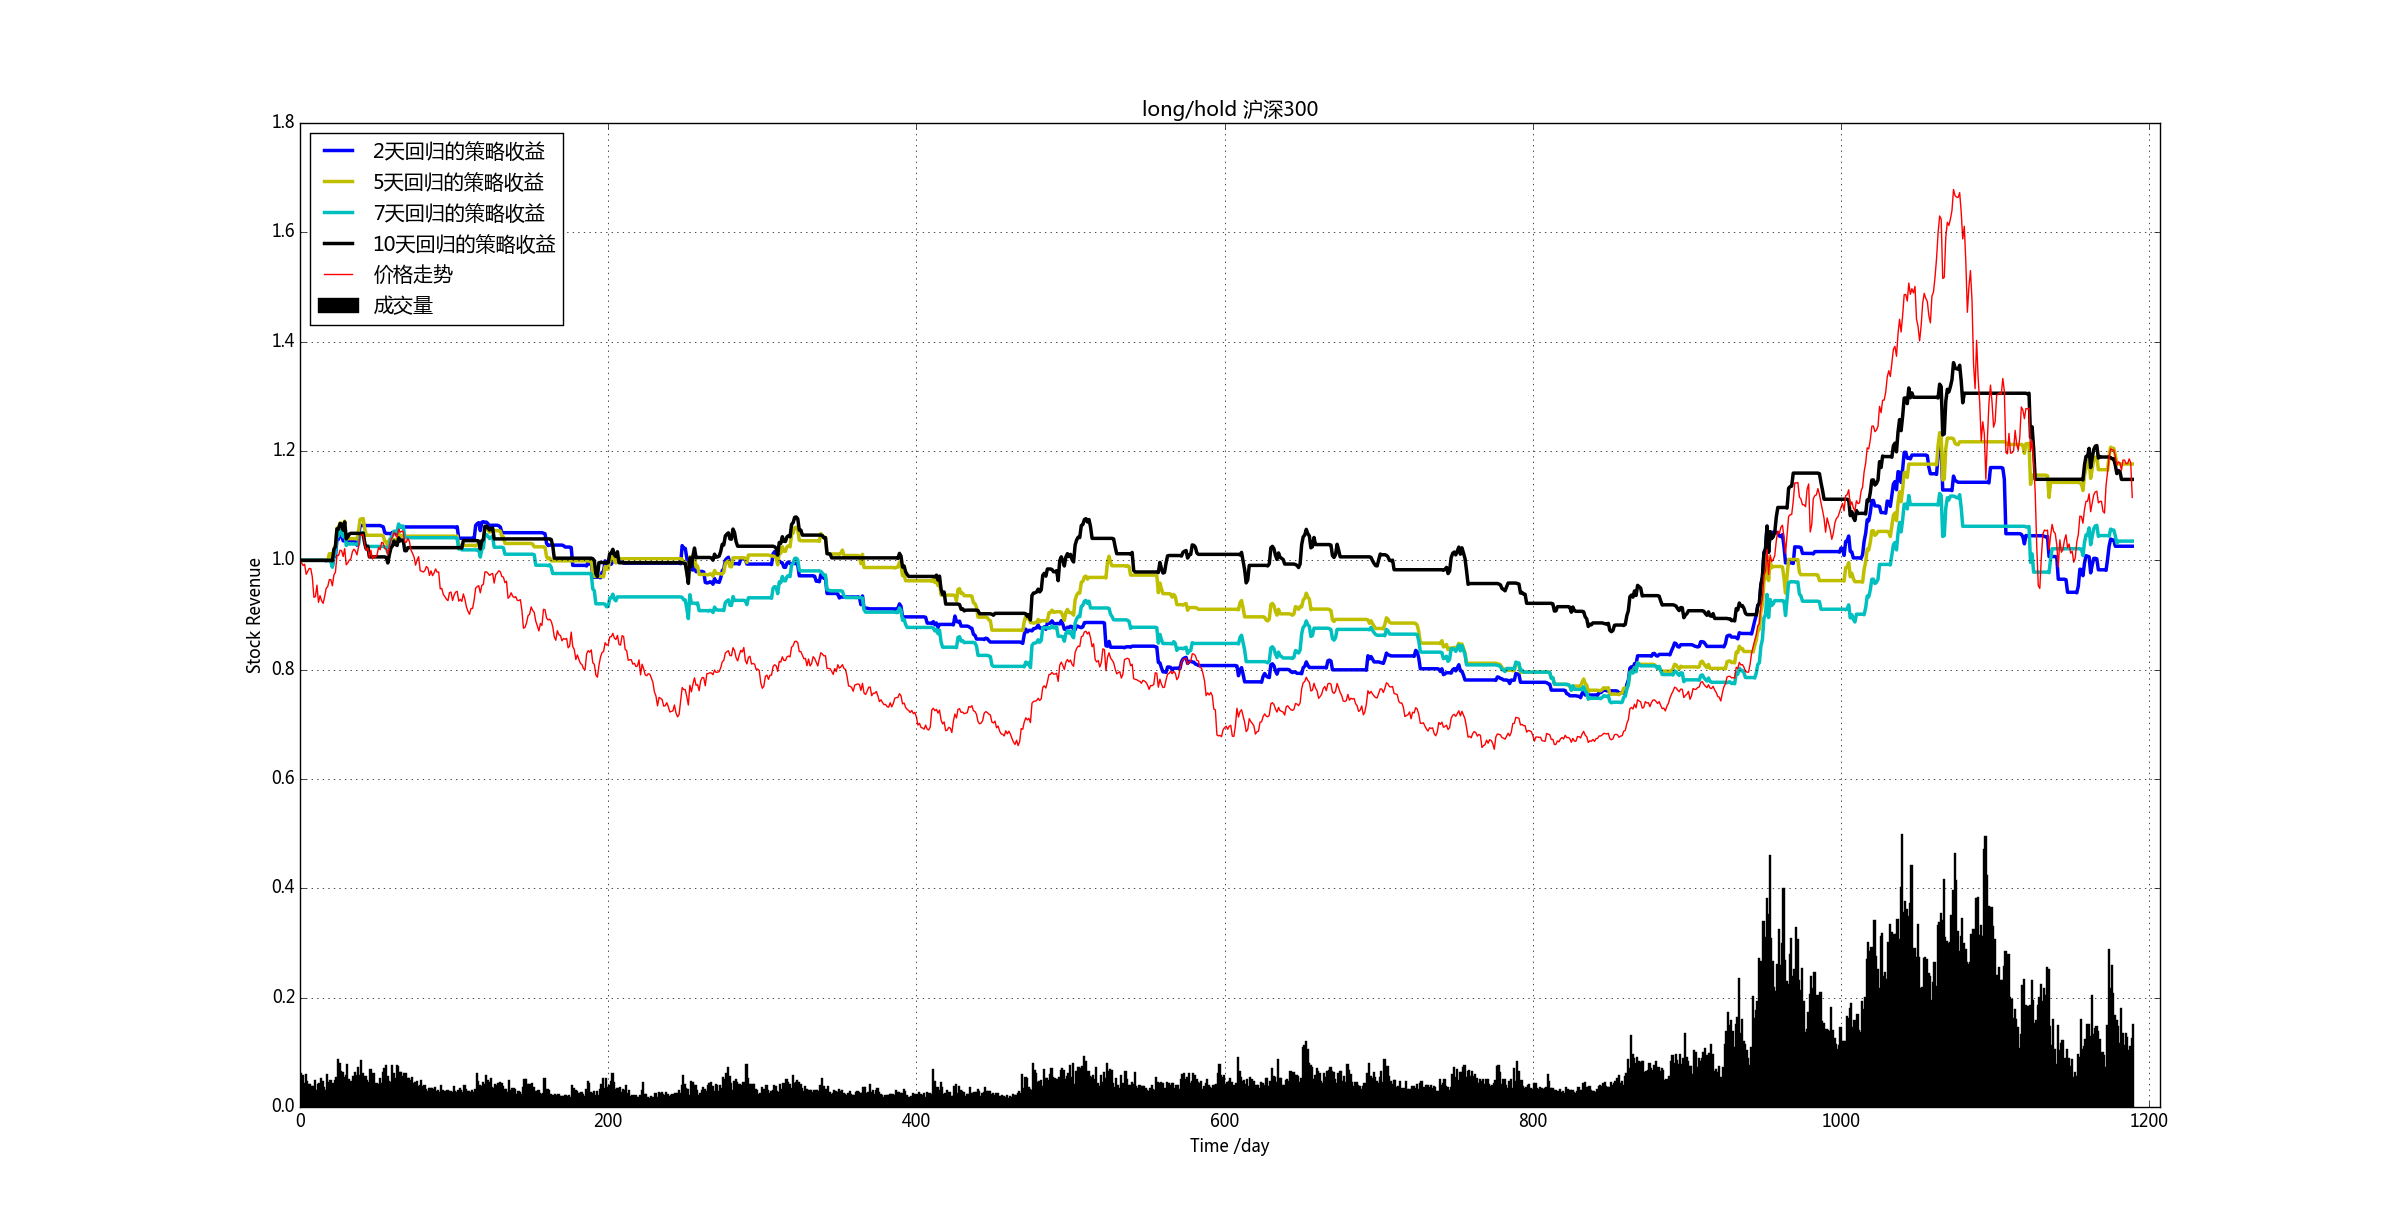
\includegraphics[width=1.0\textwidth]{img_r_5/hs300_1.png}
	\caption{沪深300 long/hold }
\end{figure}
\end{enumerate}

\subsubsection{创业板}
\begin{enumerate}
\item long/short 
\begin{figure}[H]
	\centering
	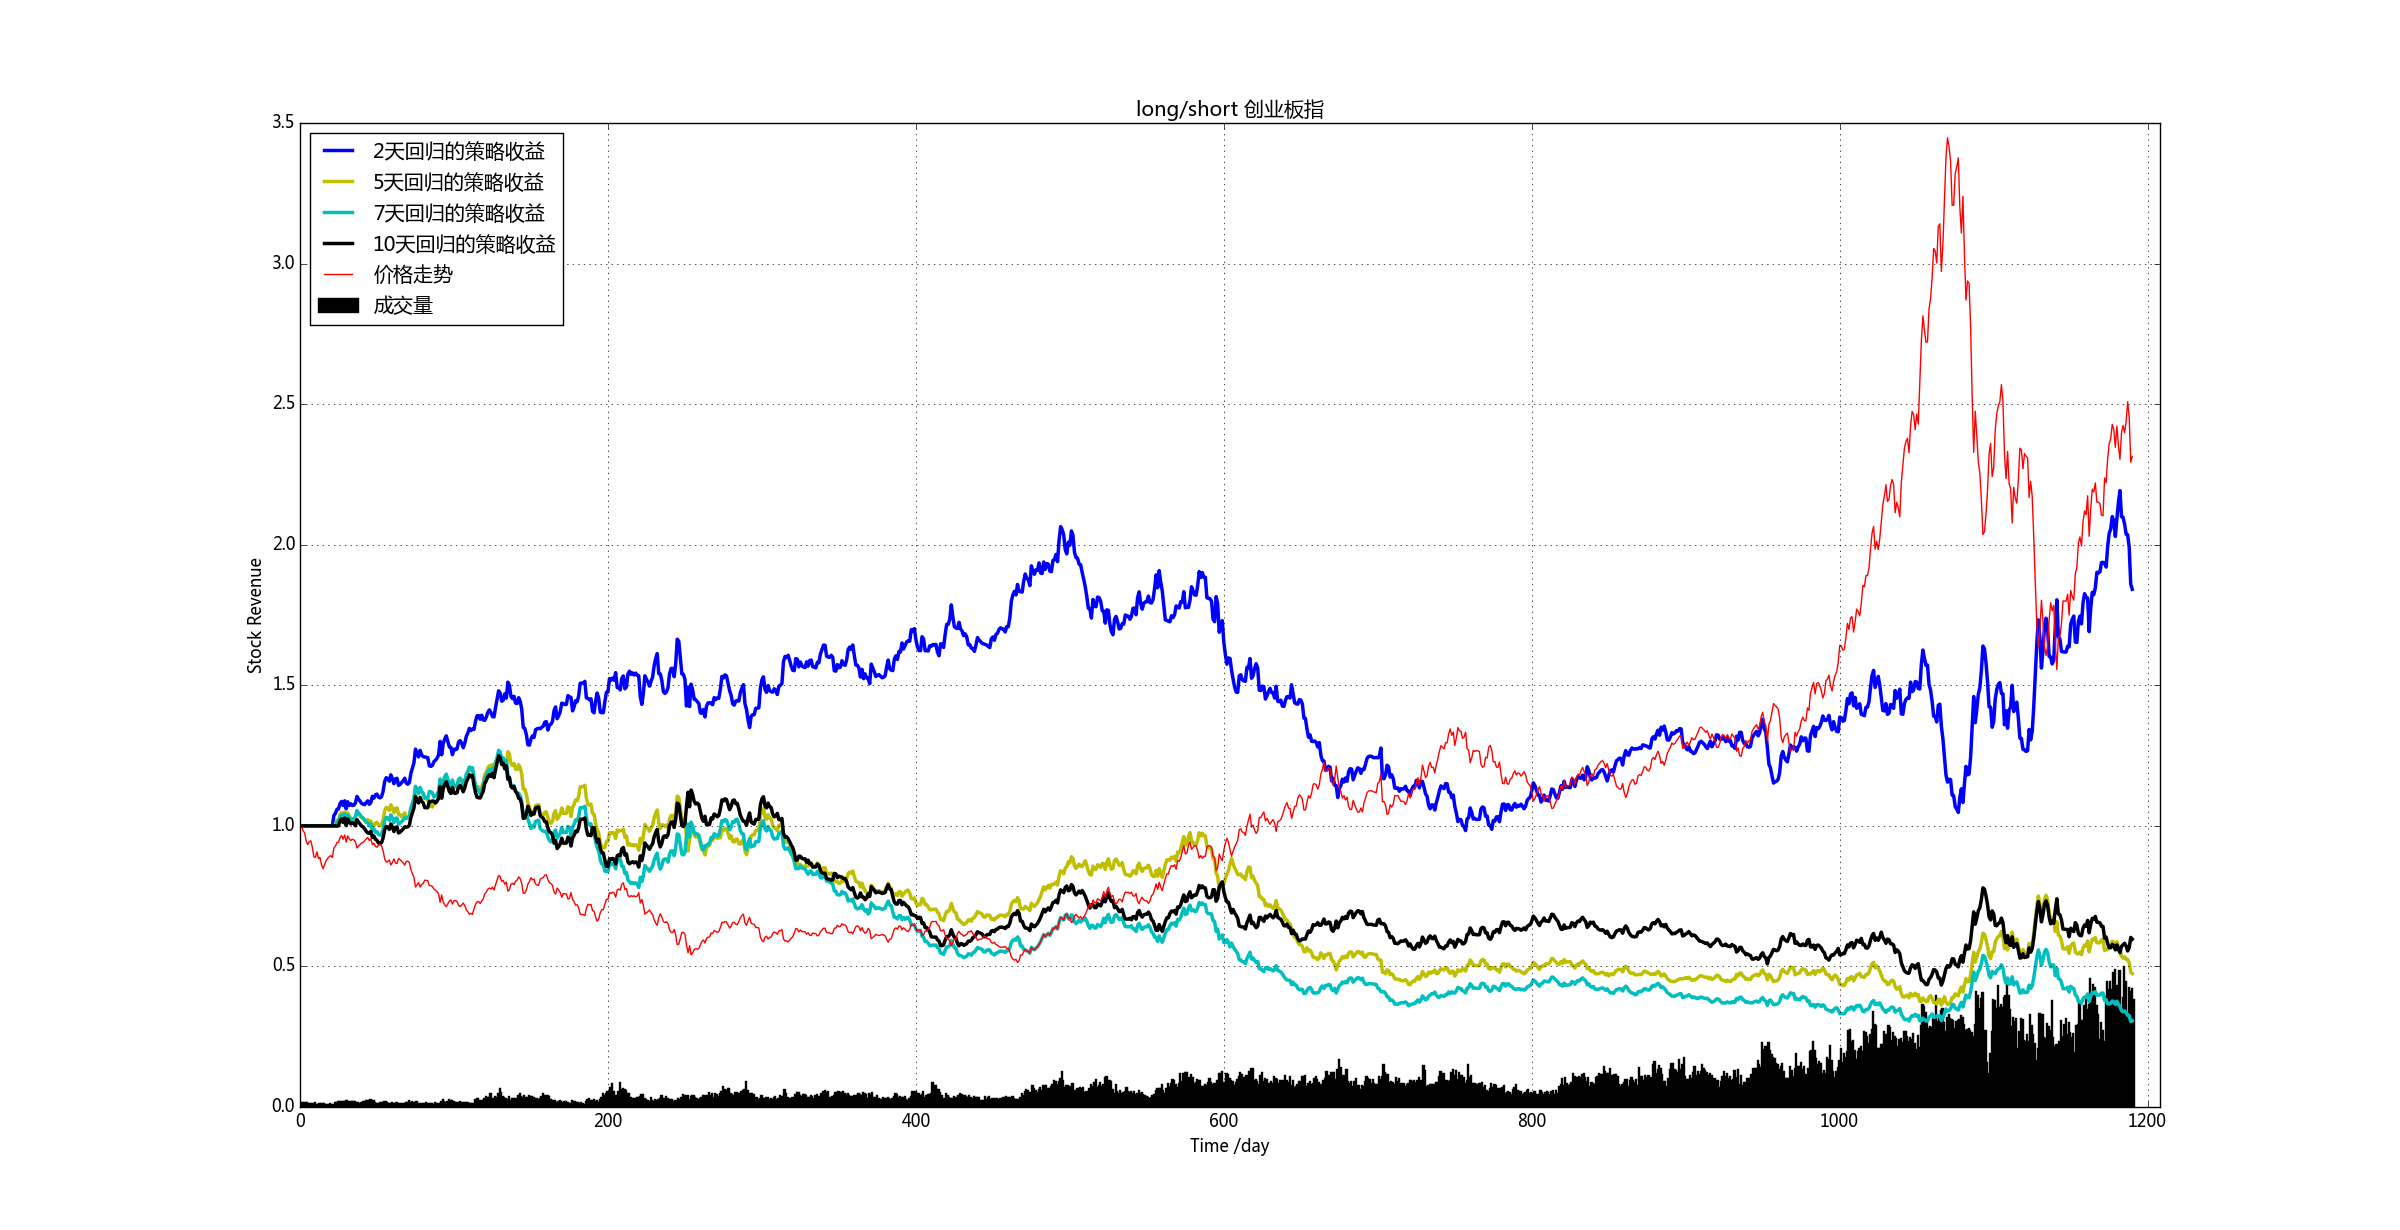
\includegraphics[width=1.0\textwidth]{img_r_5/cyb.png}
	\caption{创业板 long/short}
\end{figure}
\item long/hold 
\begin{figure}[H]
	\centering
	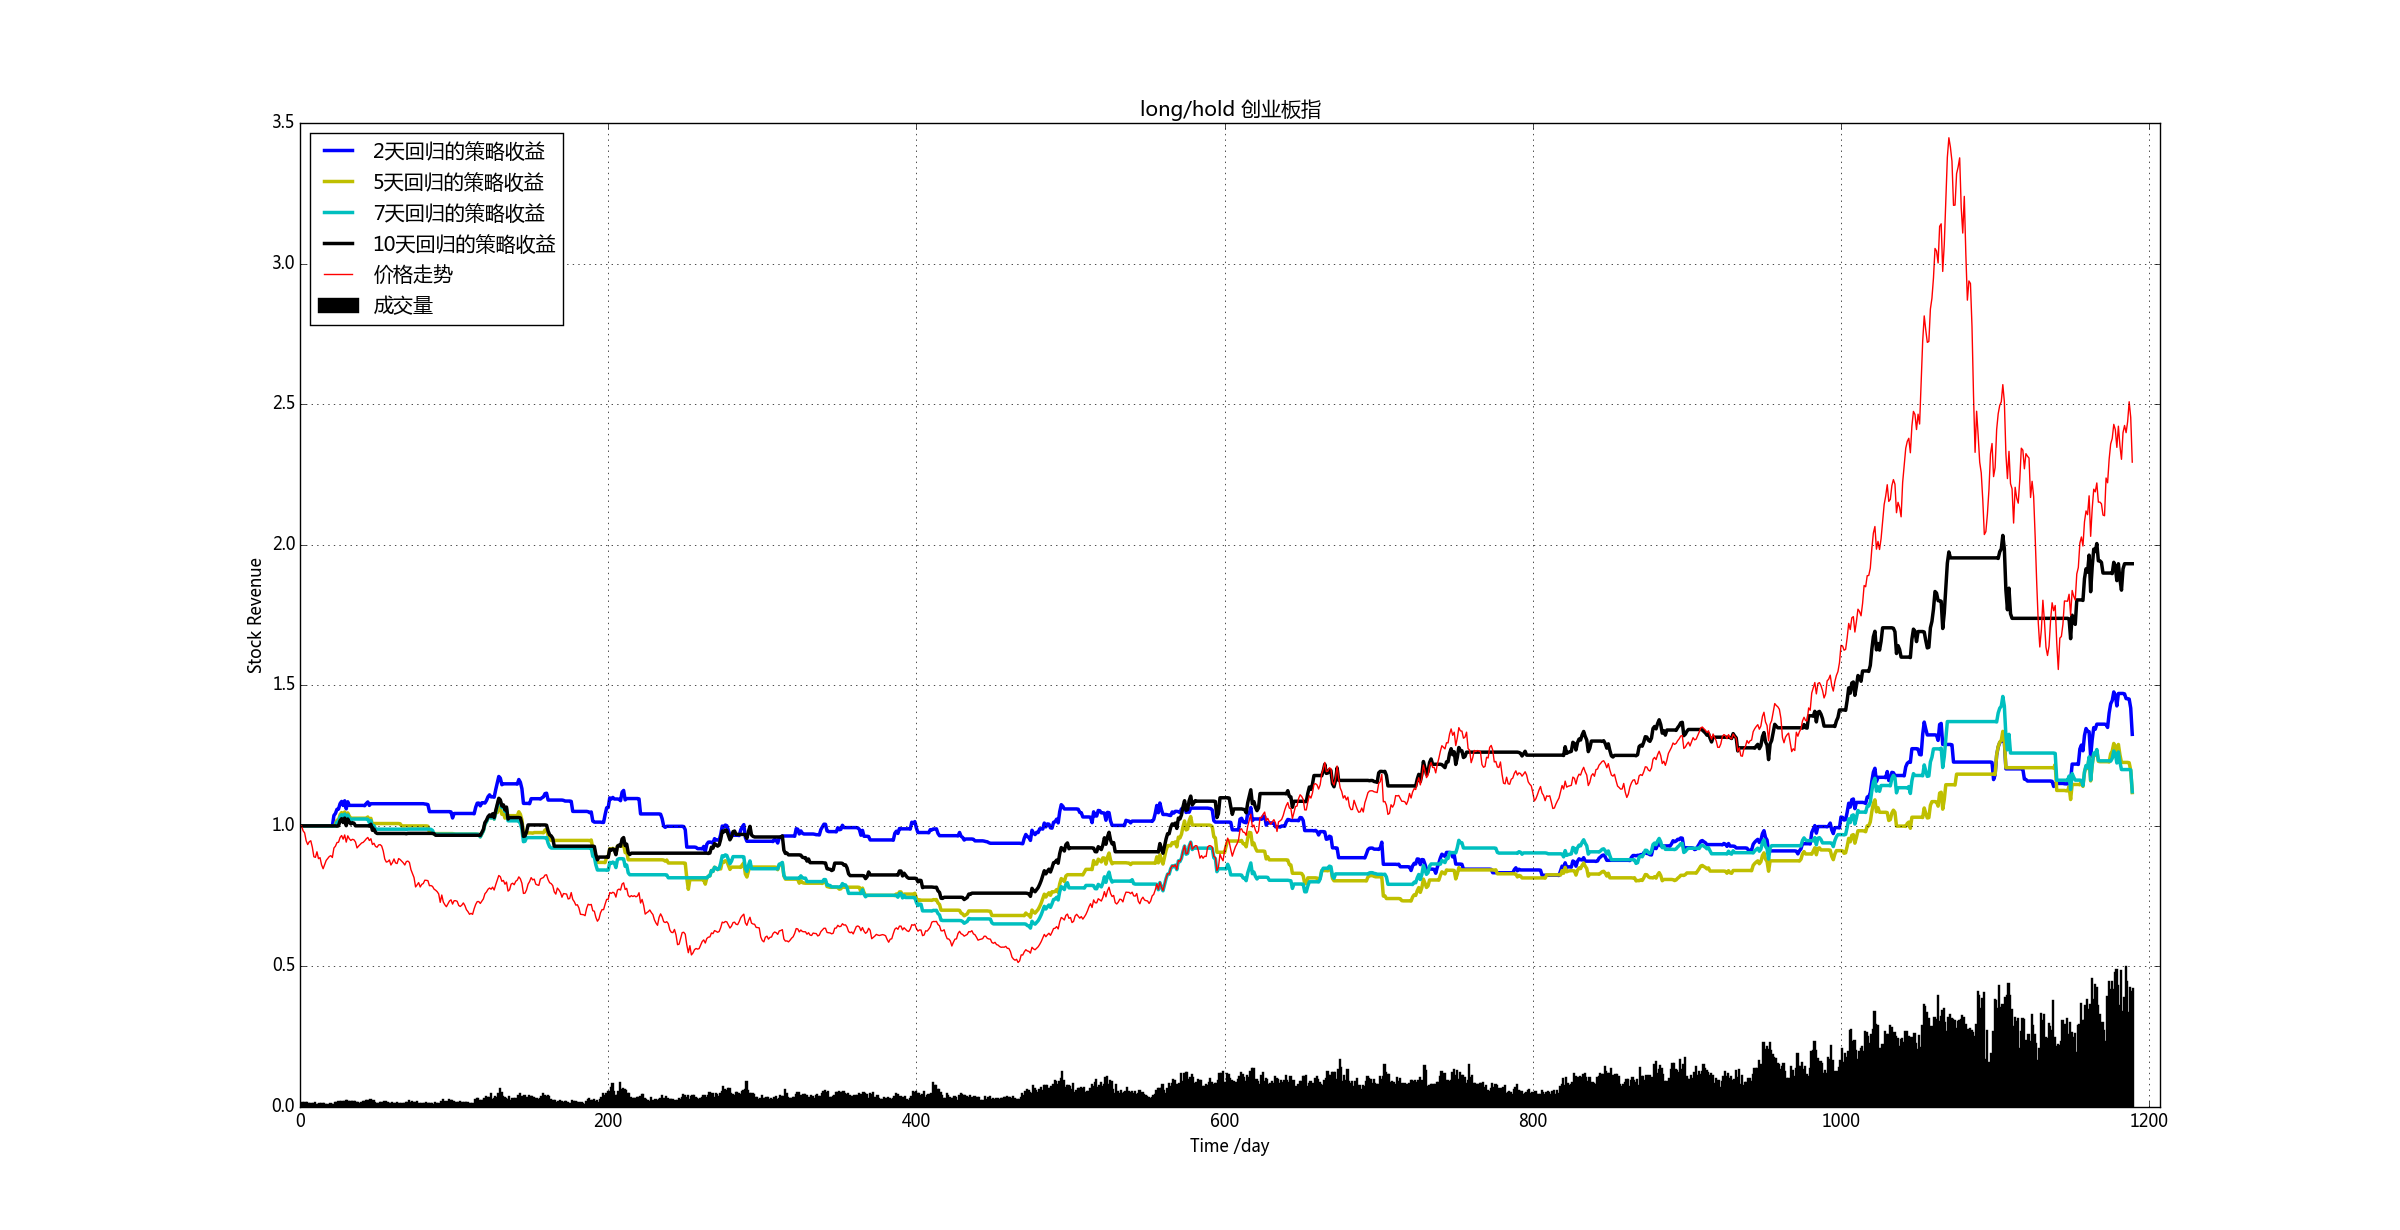
\includegraphics[width=1.0\textwidth]{img_r_5/cyb_1.png}
	\caption{创业板 long/hold }
\end{figure}
\end{enumerate}

\subsubsection{中证500}
\begin{enumerate}
\item long/short 
\begin{figure}[H]
	\centering
	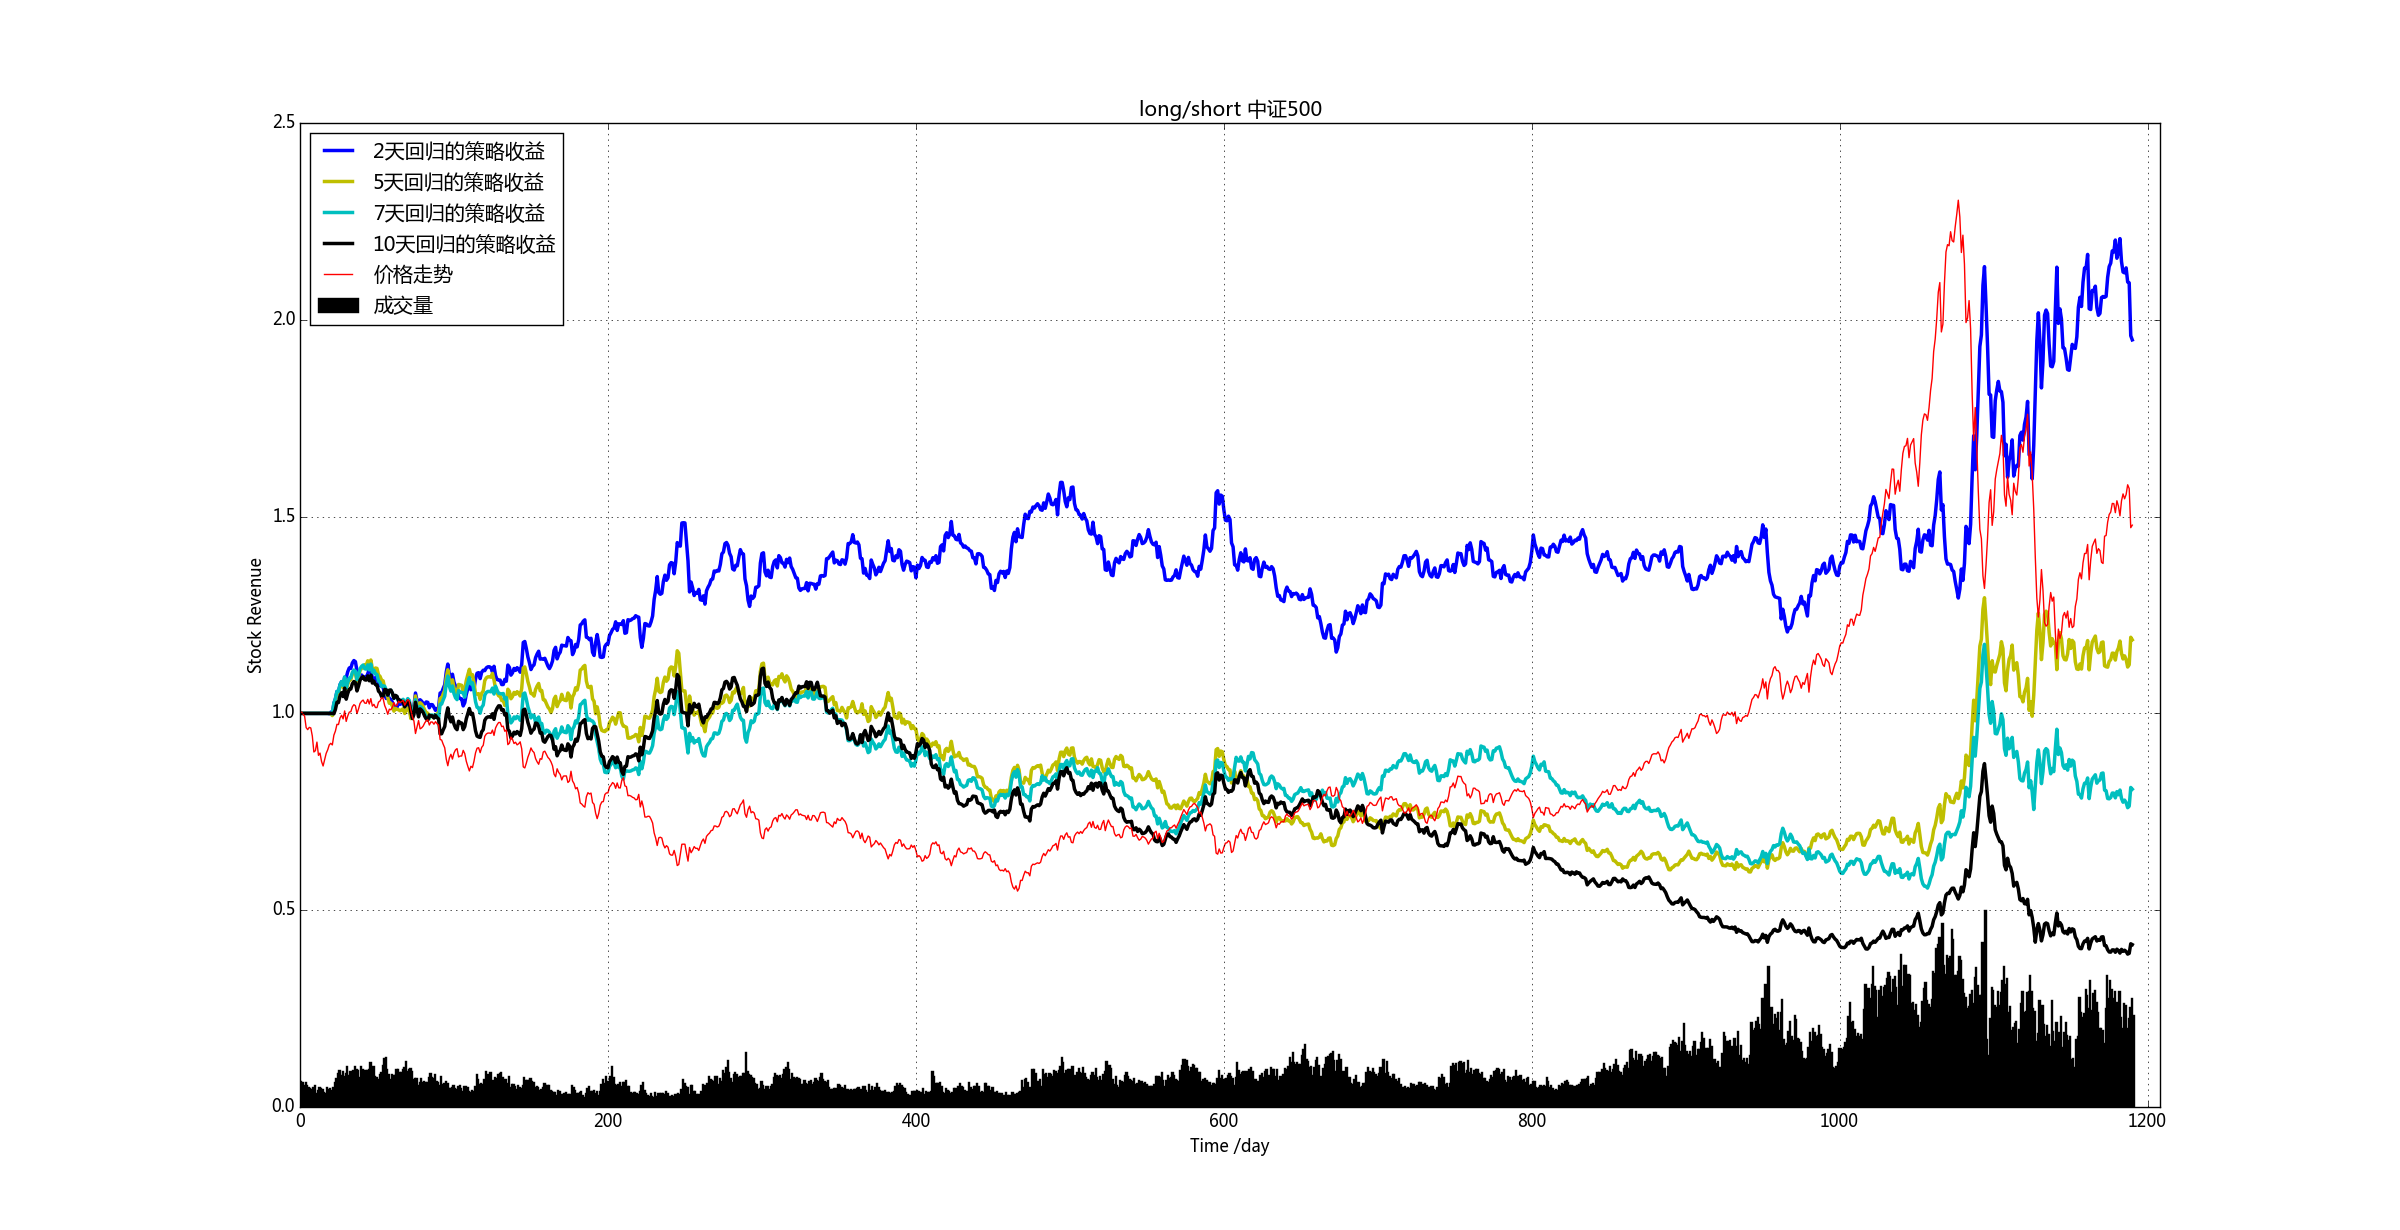
\includegraphics[width=1.0\textwidth]{img_r_5/zz500.png}
	\caption{中证500 long/short }
\end{figure}
\item long/hold 
\begin{figure}[H]
	\centering
	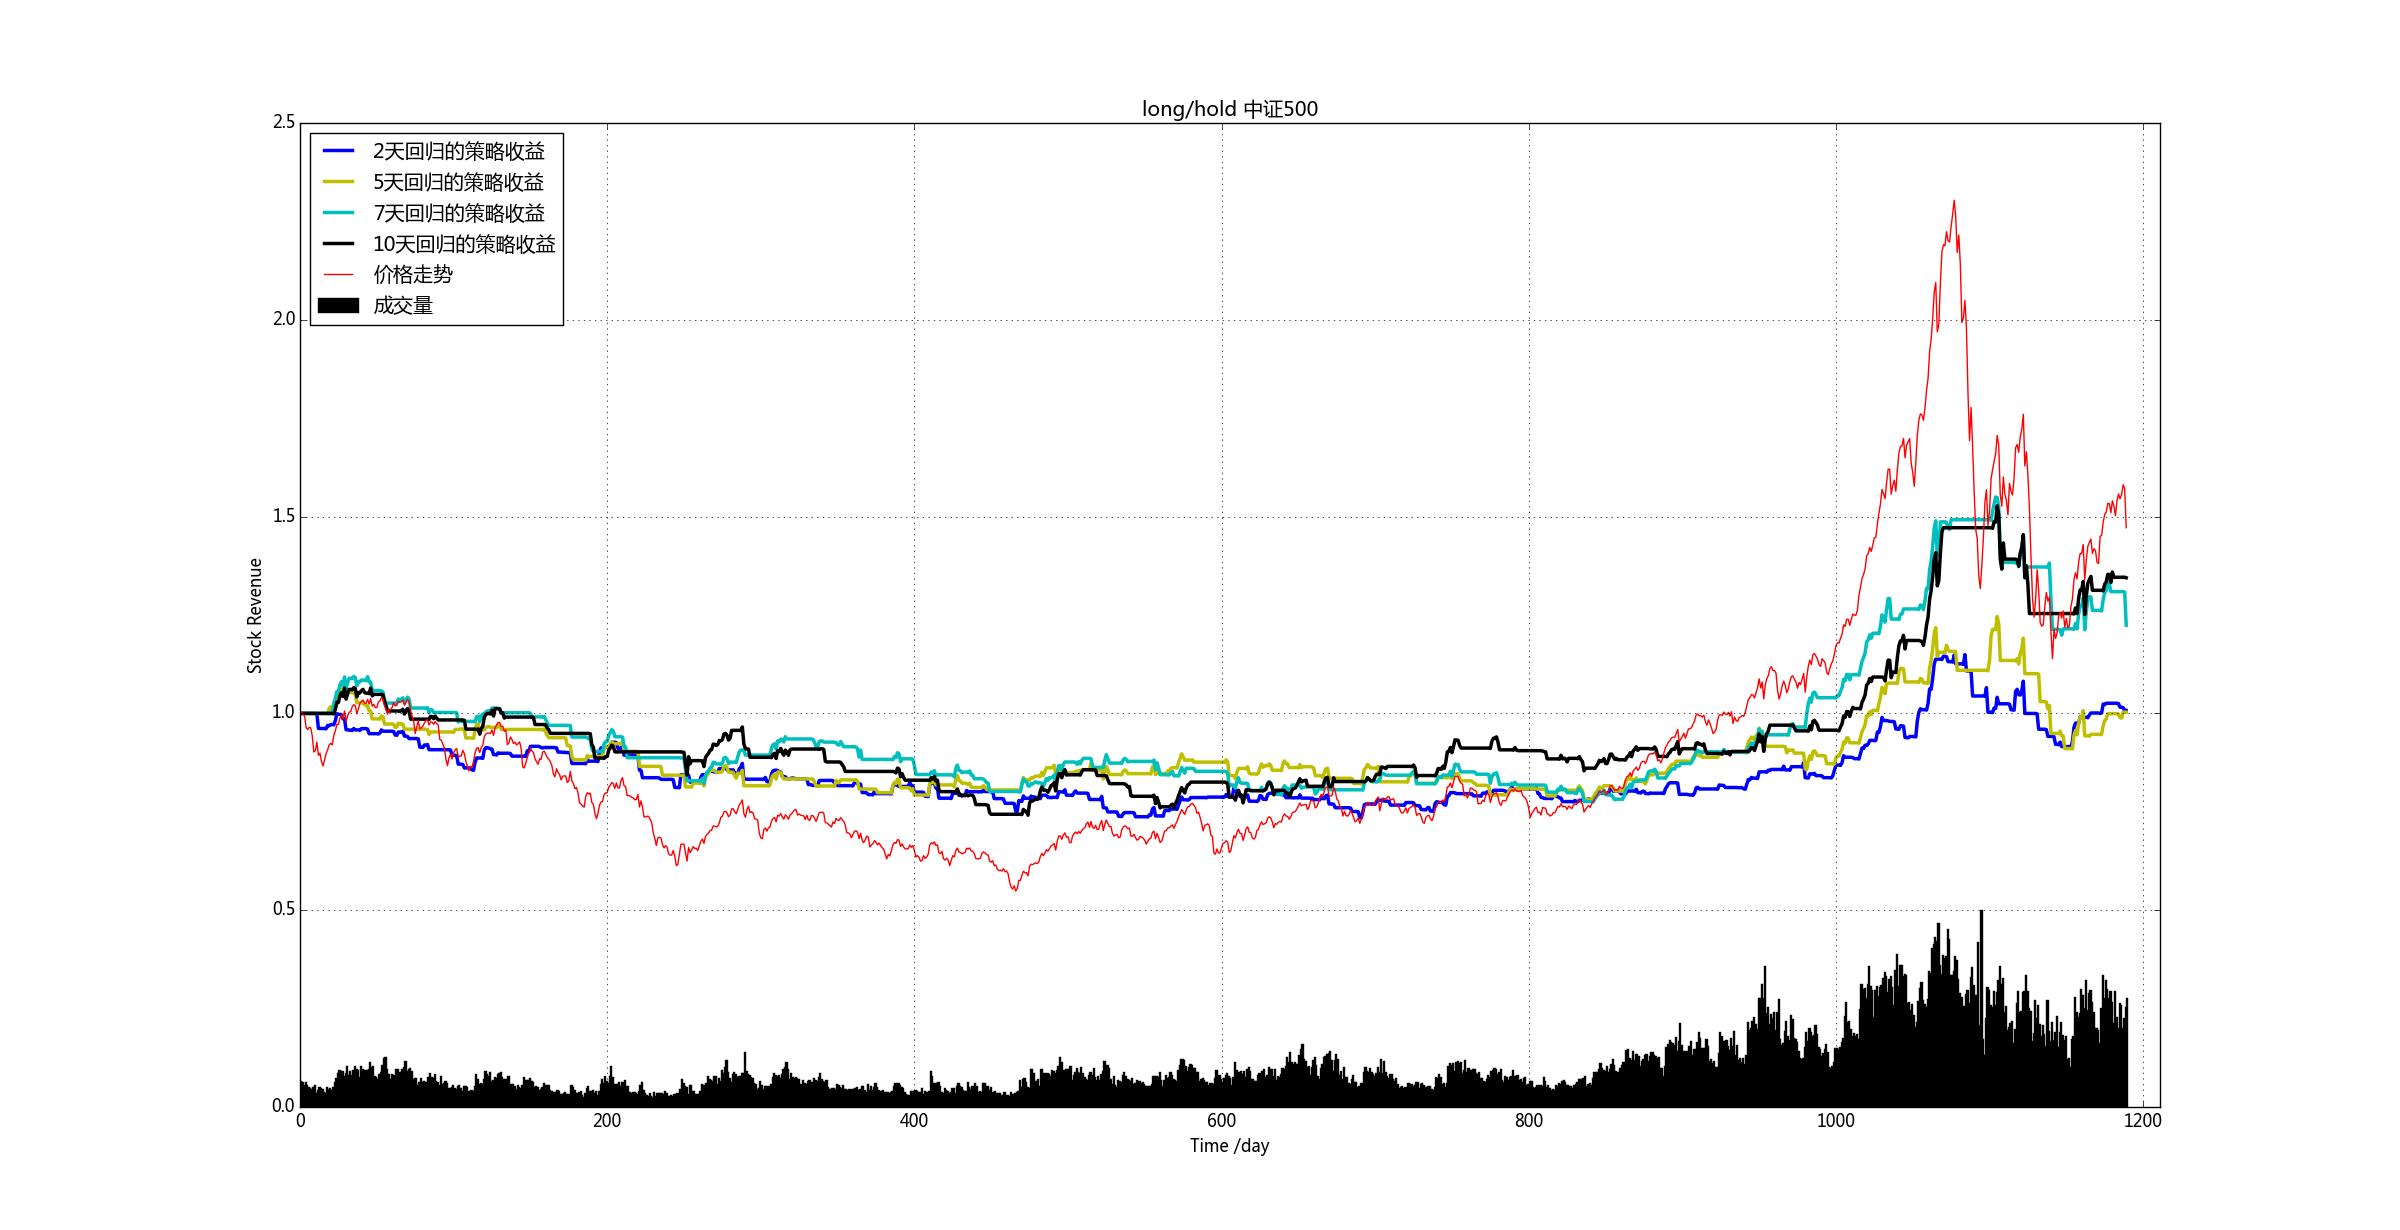
\includegraphics[width=1.0\textwidth]{img_r_1/zz500_1.png}
	\caption{中证500 long/hold}
\end{figure}
\end{enumerate}


\subsection{价格和成交量7日MA}
\subsubsection{上证50}

\begin{enumerate}
\item long/short 
\begin{figure}[H]
	\centering
	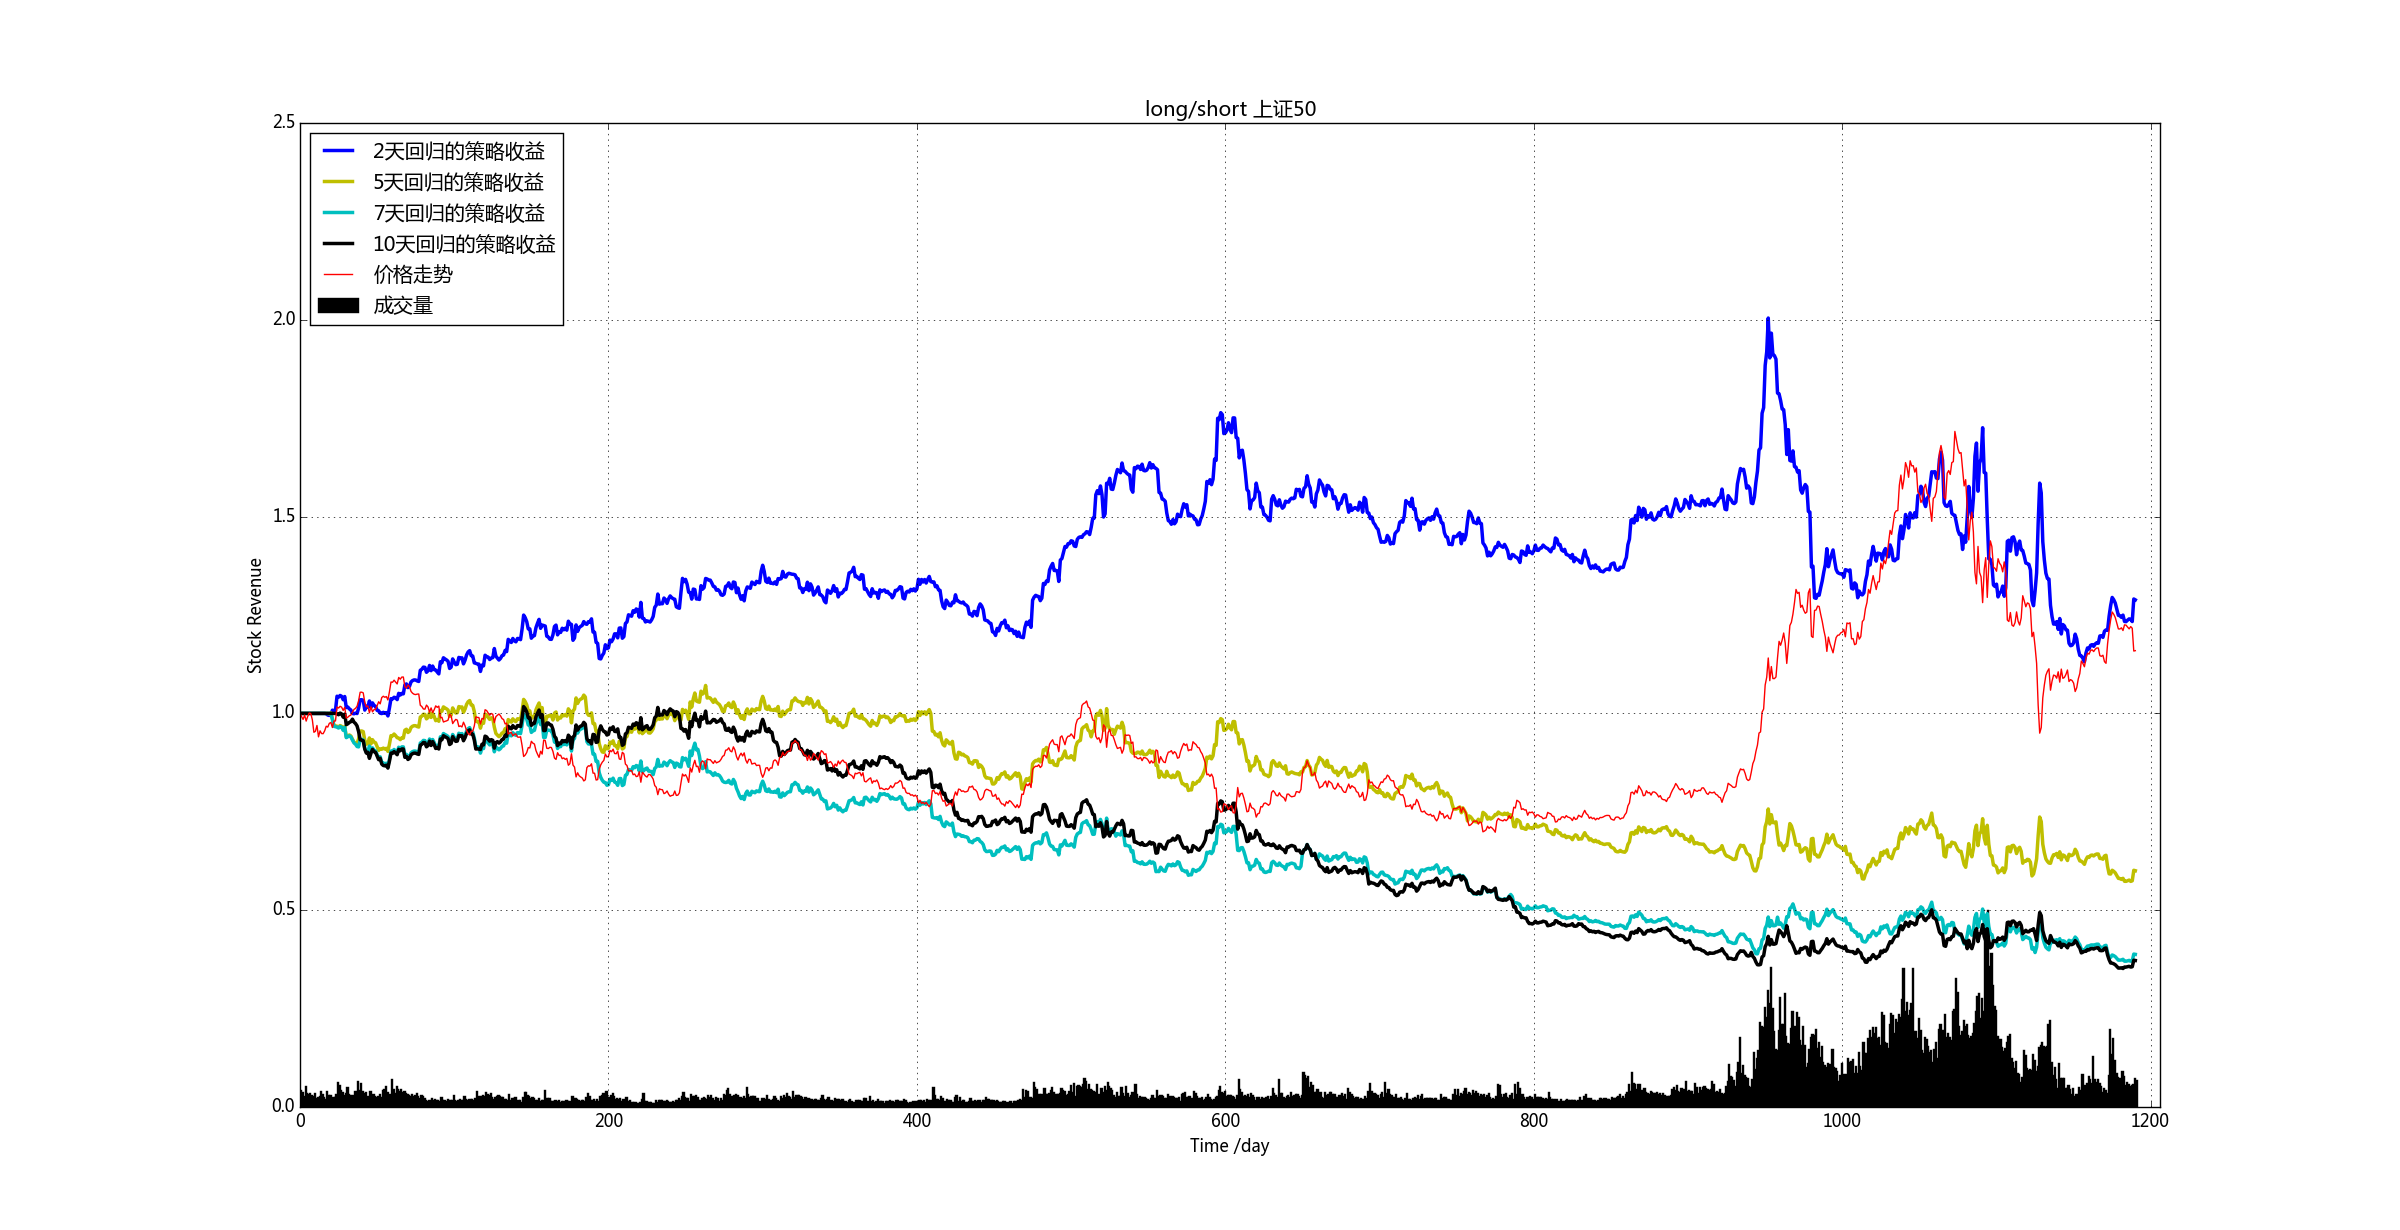
\includegraphics[width=1.0\textwidth]{img_r_7/sz50.png}
	\caption{上证50 long/short}
\end{figure}

\item long/hold 
\begin{figure}[H]
	\centering
	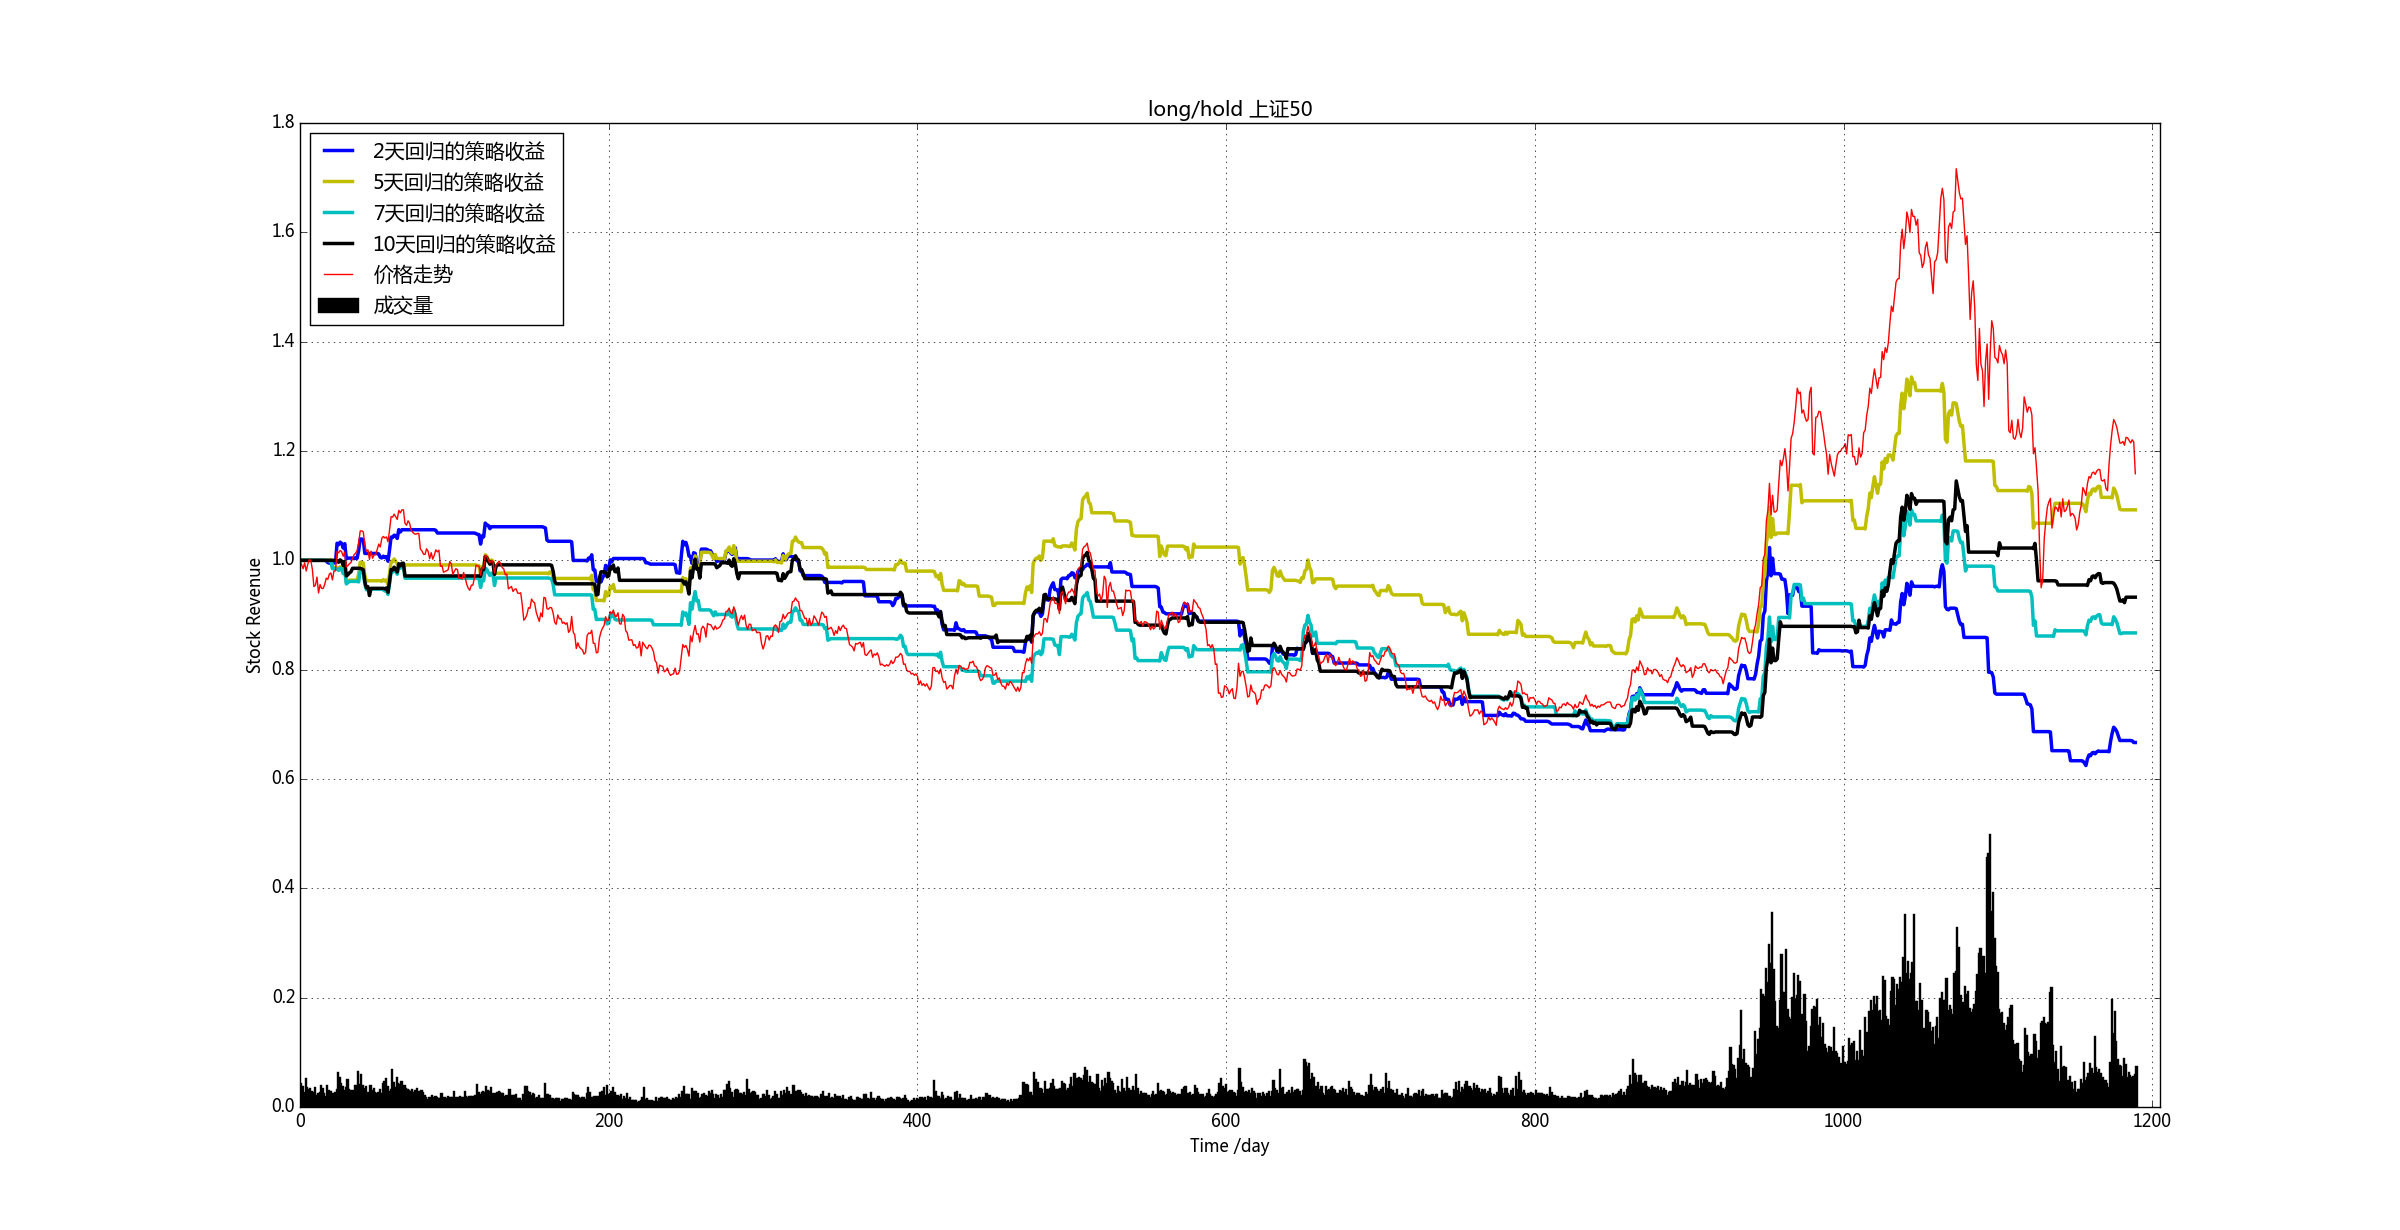
\includegraphics[width=1.0\textwidth]{img_r_7/sz50_1.png}
	\caption{上证50 long/hold}
\end{figure}
\end{enumerate}

\subsubsection{上证综指}

\begin{enumerate}
\item long/short 
\begin{figure}[H]
	\centering
	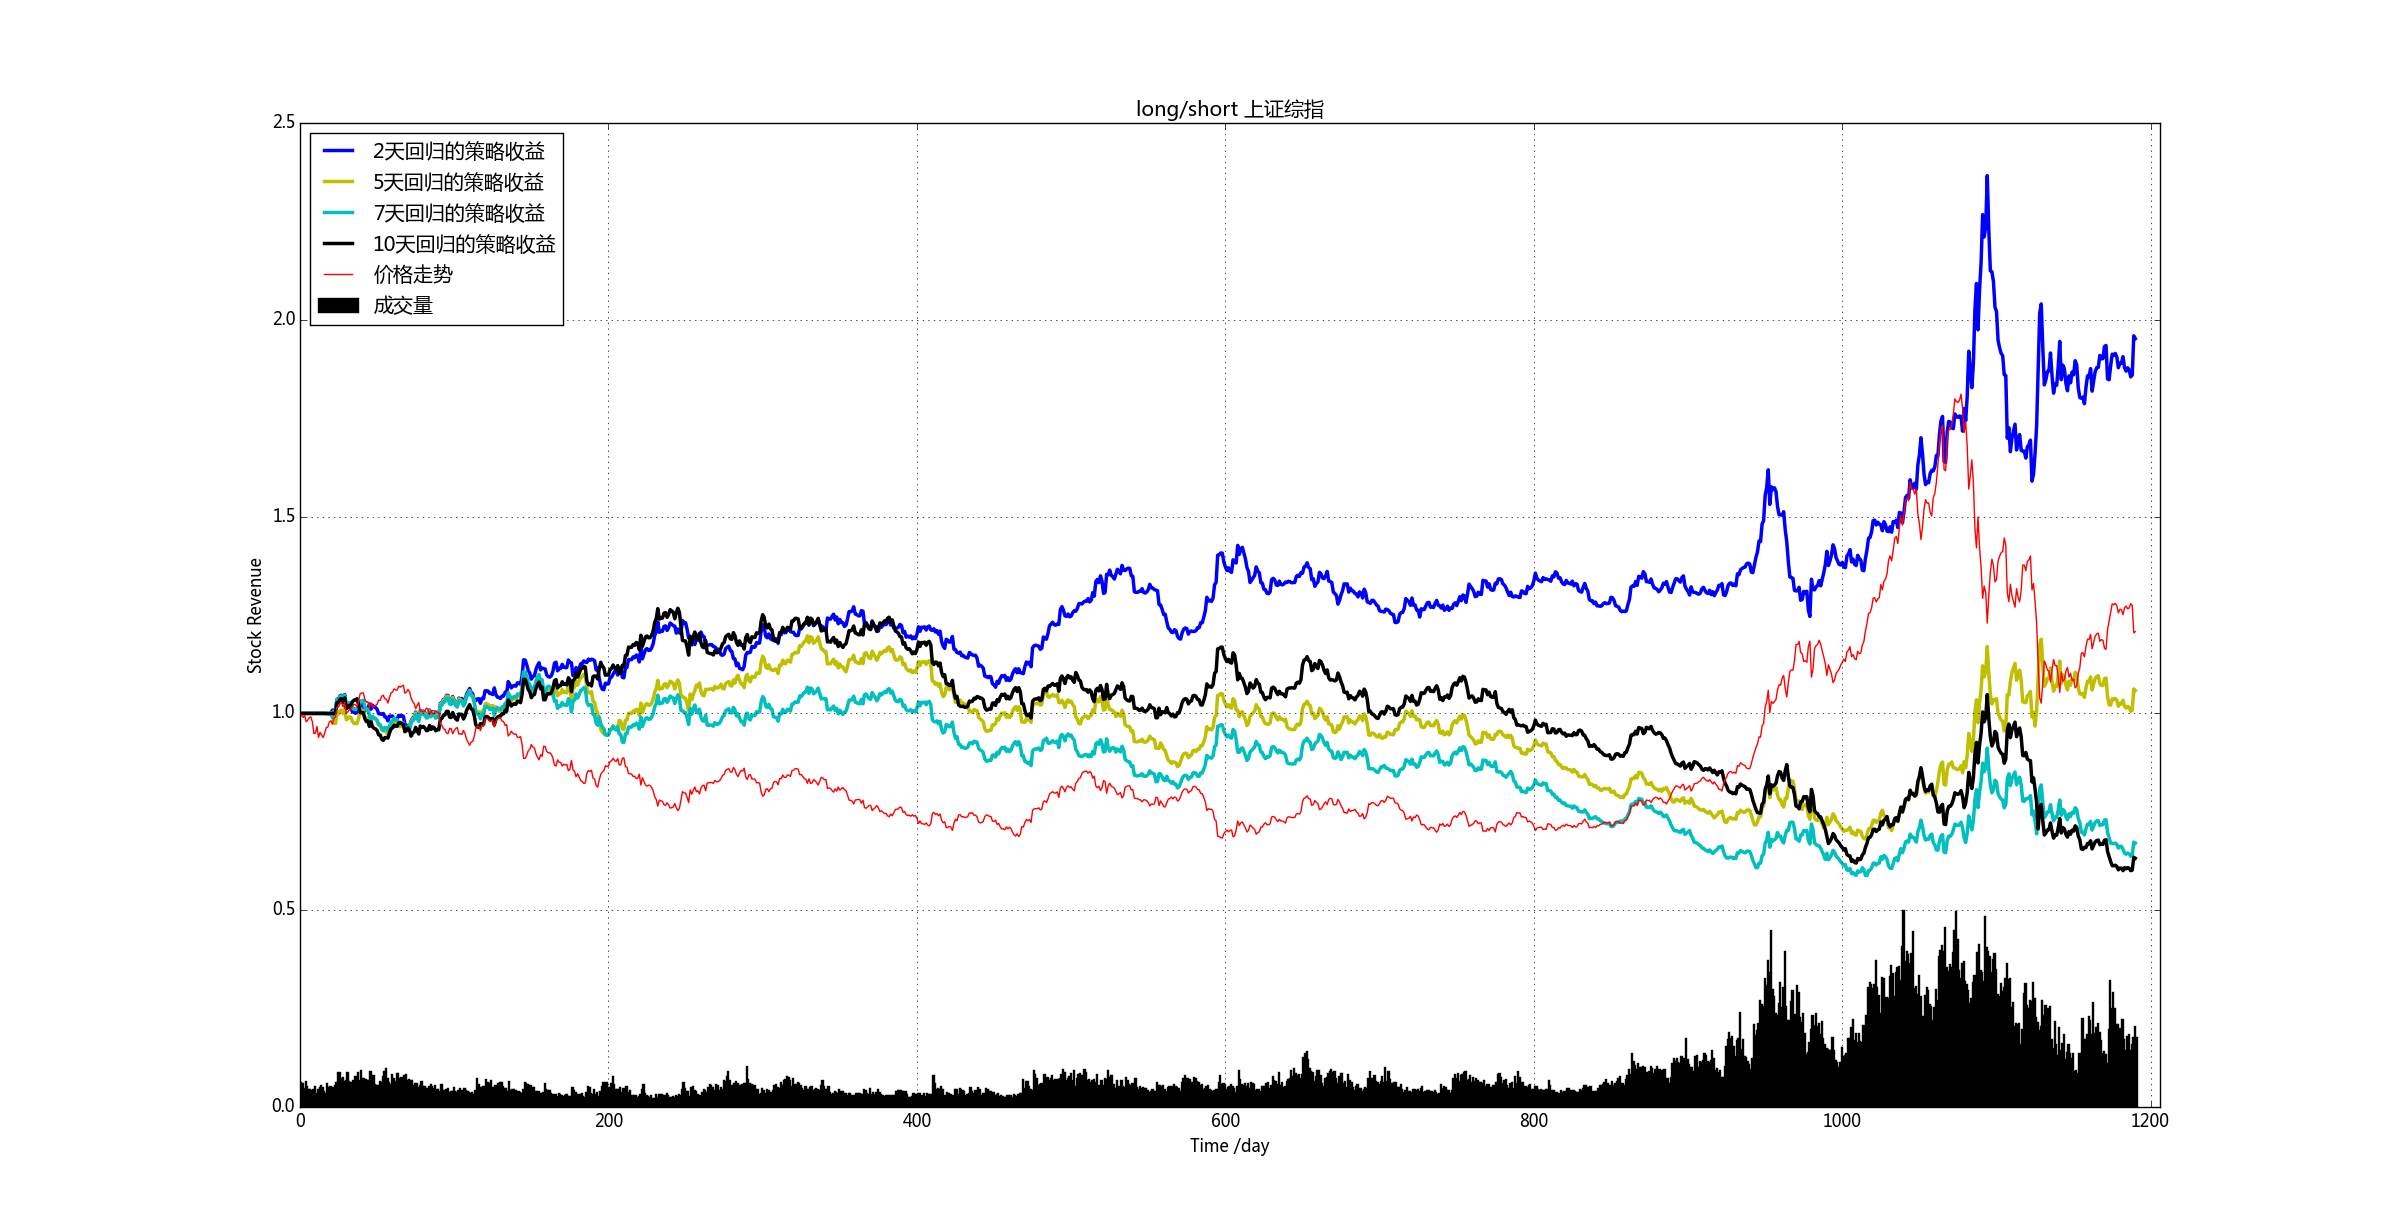
\includegraphics[width=1.0\textwidth]{img_r_7/szzz.png}
	\caption{上证综指 long/short}
\end{figure}
\item long/hold 
\begin{figure}[H]
	\centering
	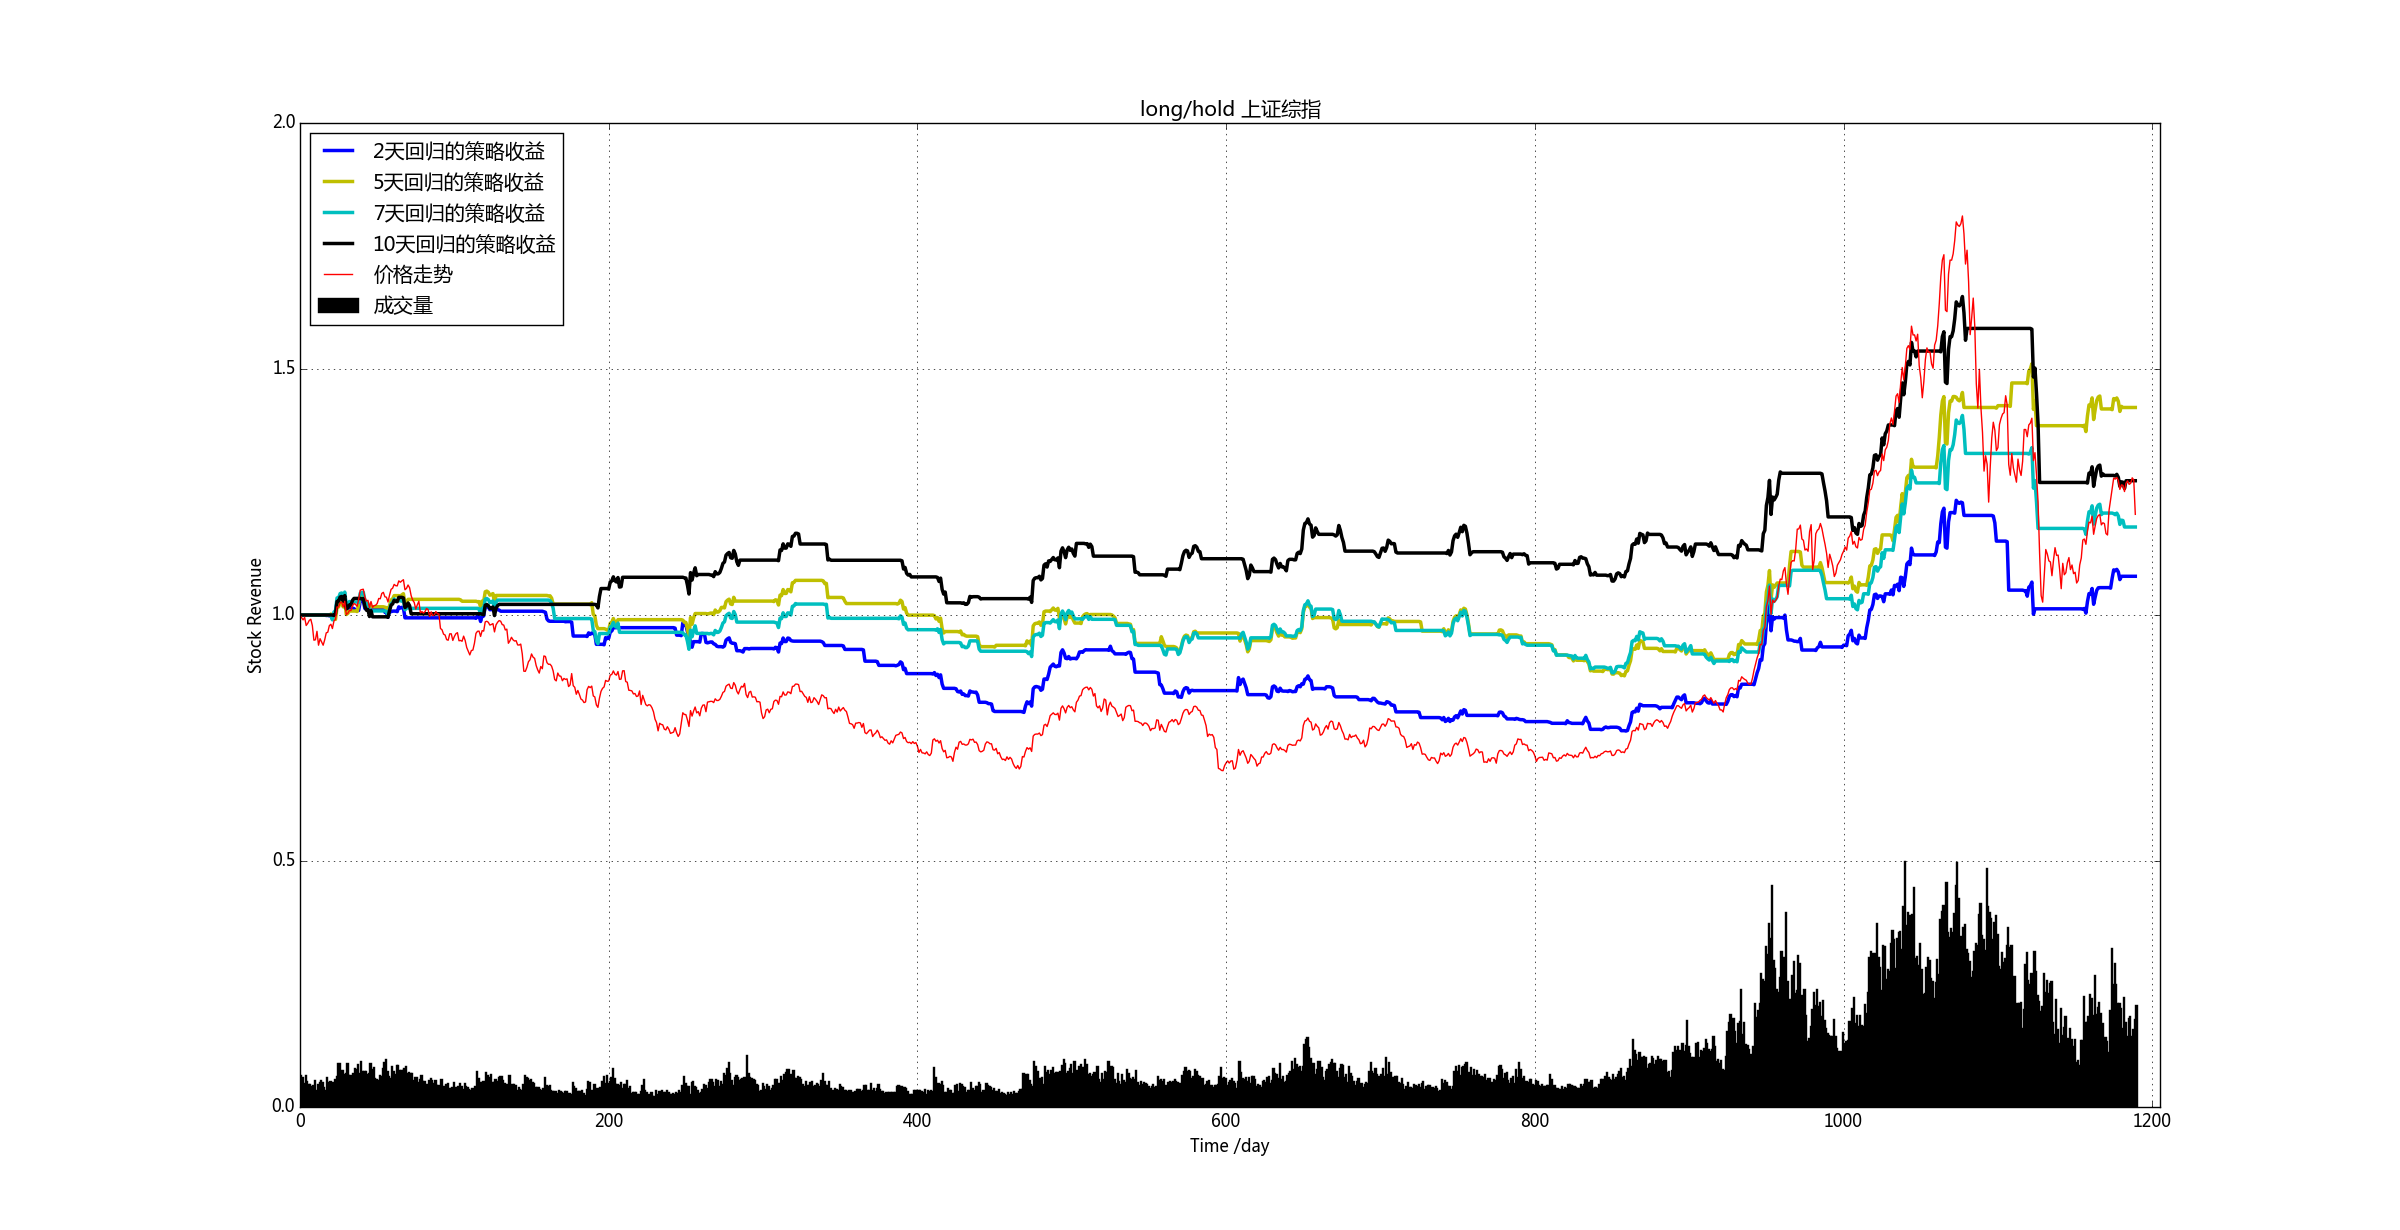
\includegraphics[width=1.0\textwidth]{img_r_7/szzz_1.png}
	\caption{上证综指 long/hold}
\end{figure}
\end{enumerate}

\subsubsection{沪深300}
\begin{enumerate}
\item long/short 
\begin{figure}[H]
	\centering
	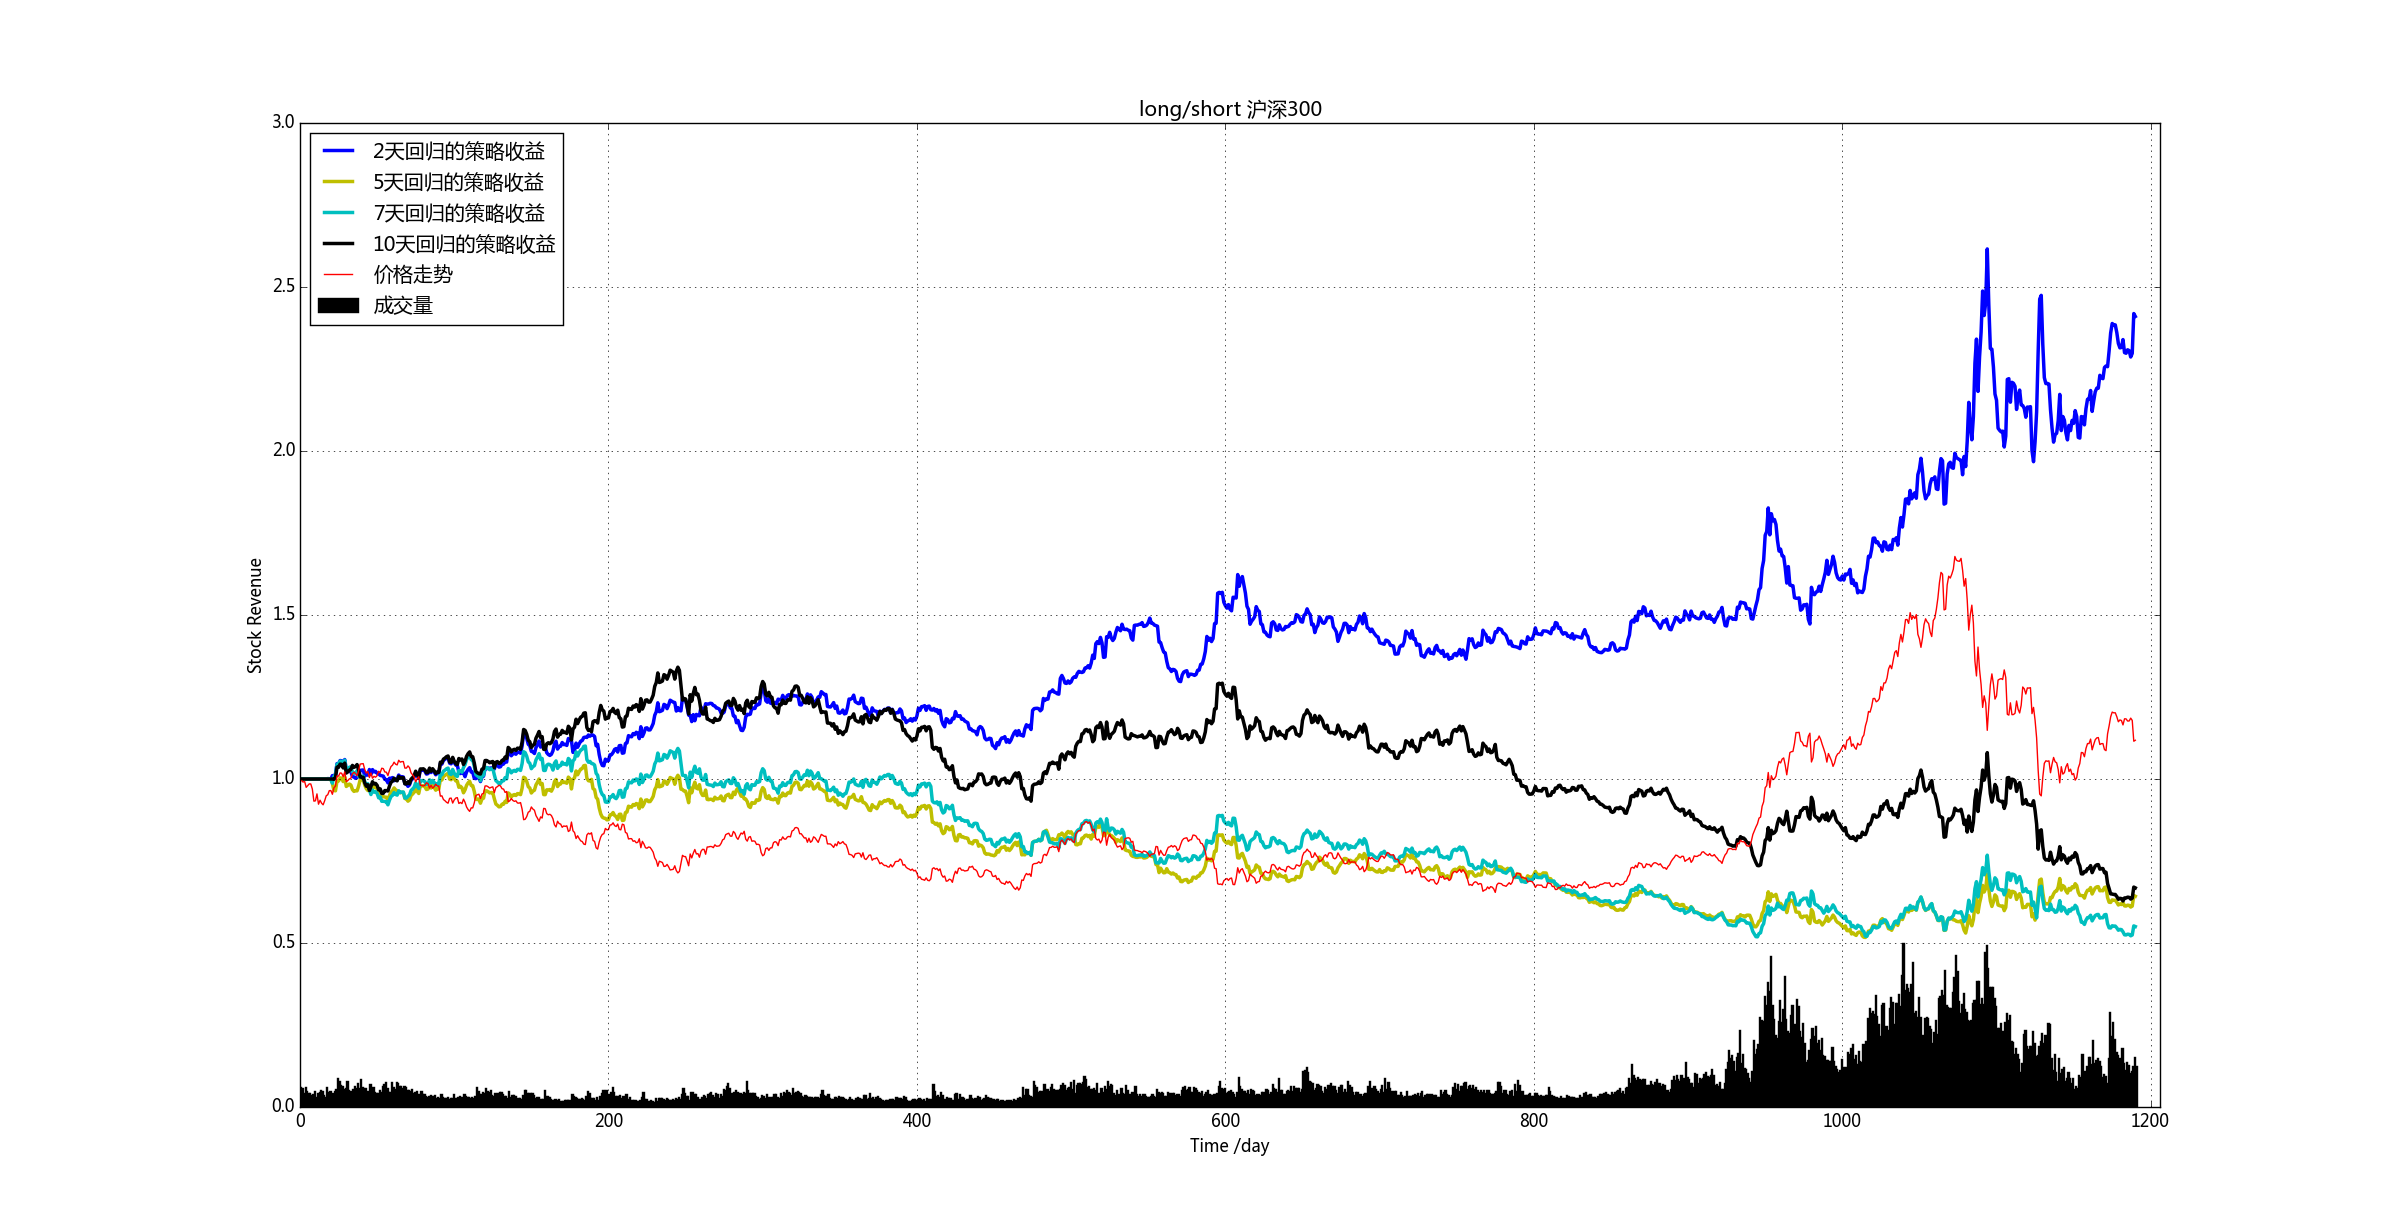
\includegraphics[width=1.0\textwidth]{img_r_7/hs300.png}
	\caption{沪深300 long/short }
\end{figure}
\item long/hold 
\begin{figure}[H]
	\centering
	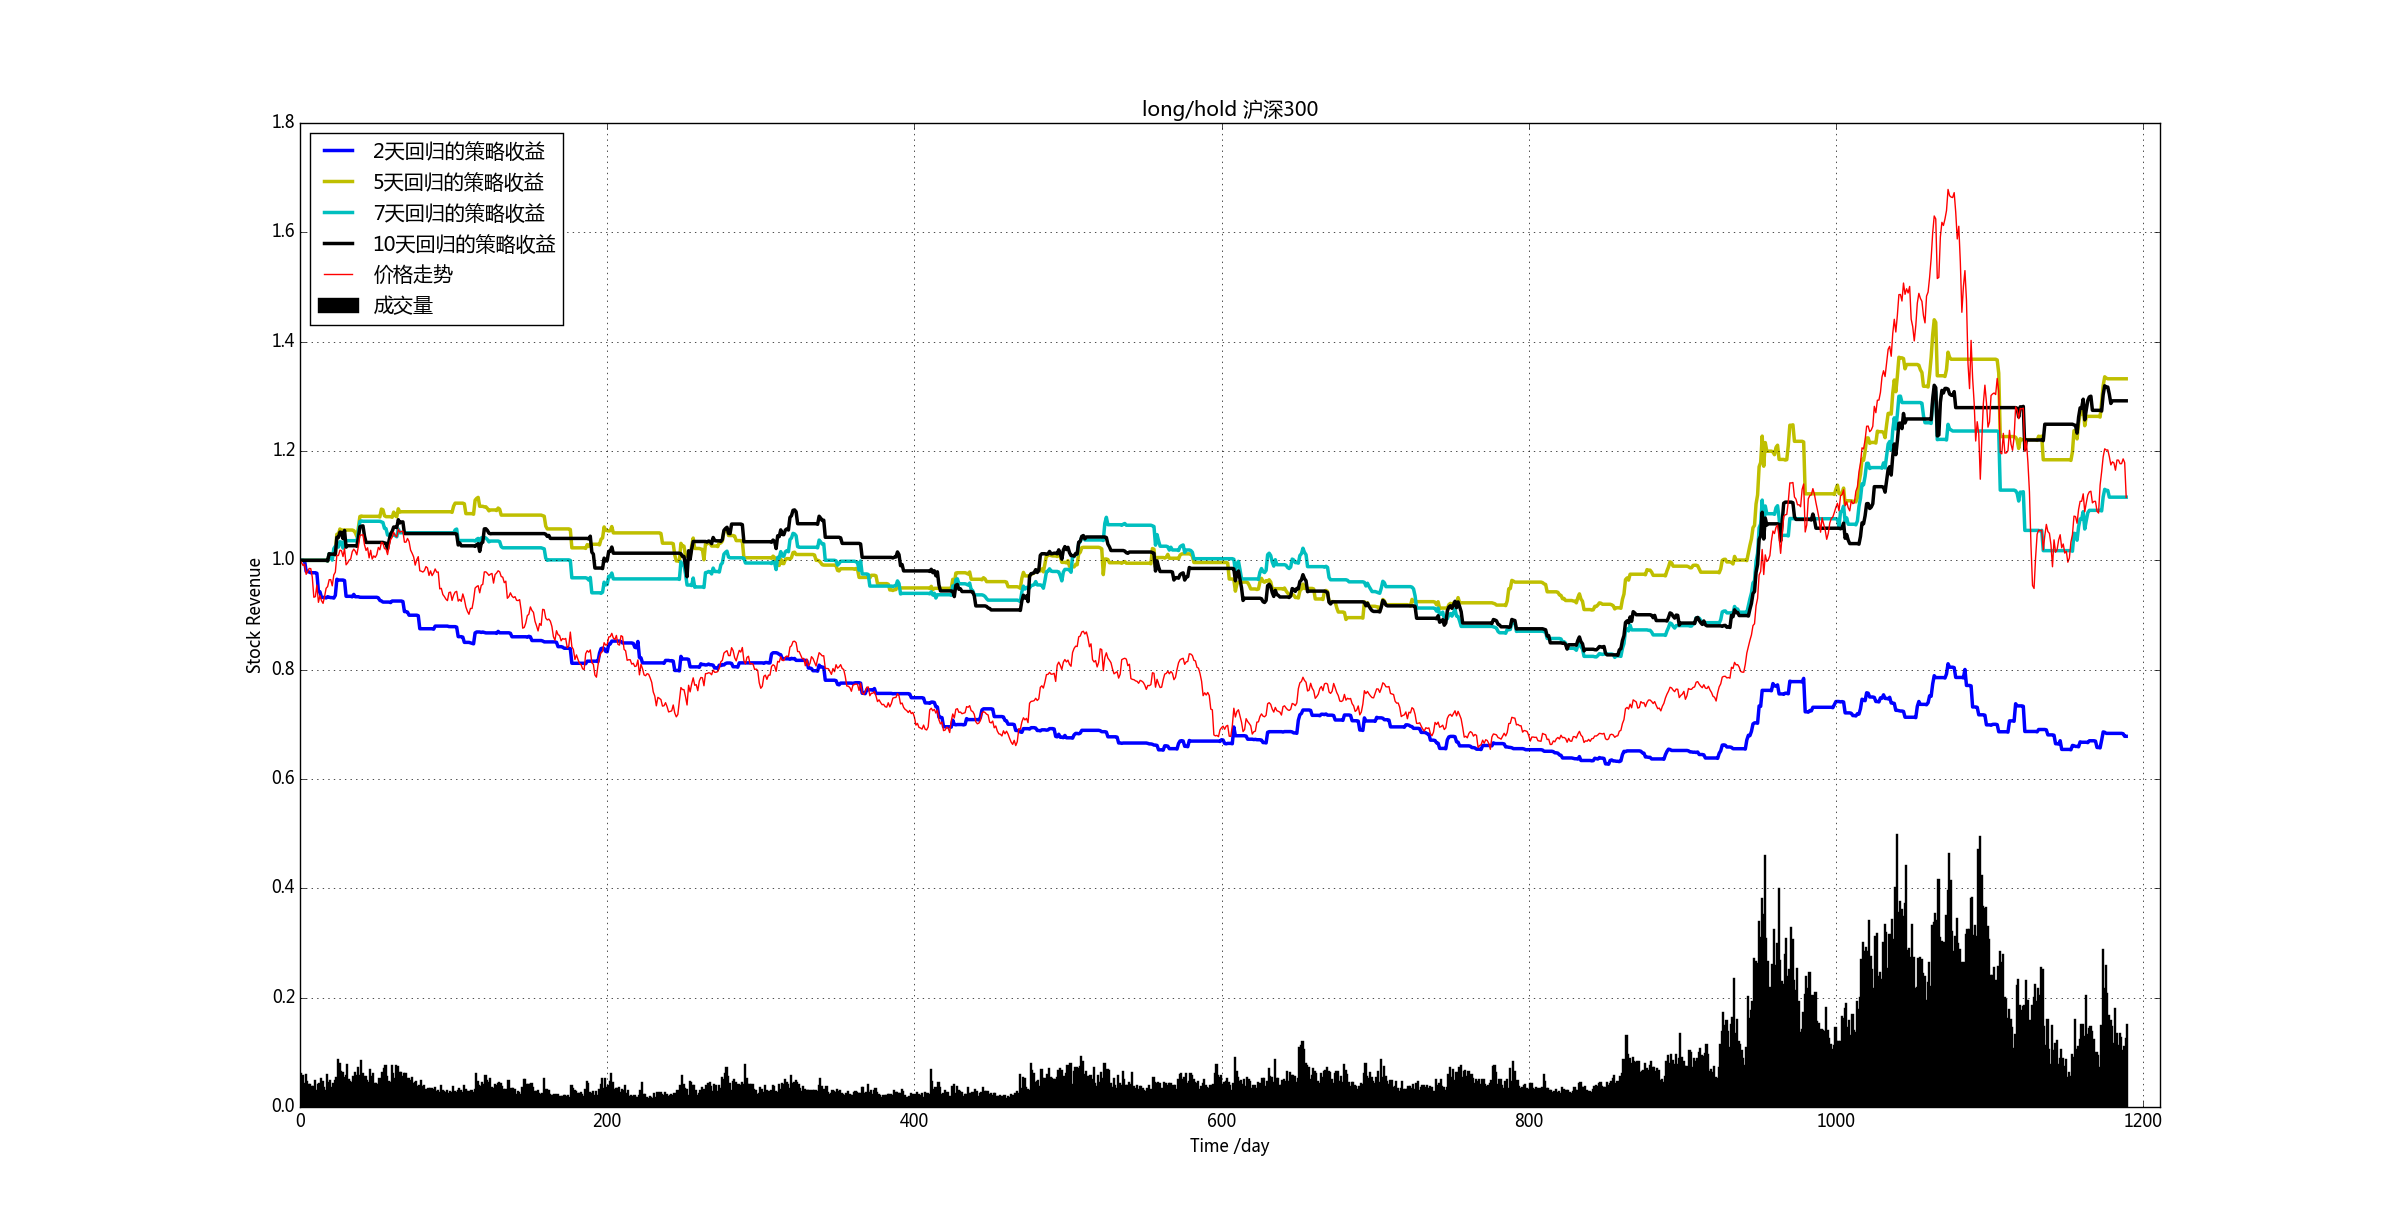
\includegraphics[width=1.0\textwidth]{img_r_1/hs300_1.png}
	\caption{沪深300 long/hold }
\end{figure}
\end{enumerate}

\subsubsection{创业板}
\begin{enumerate}
\item long/short 
\begin{figure}[H]
	\centering
	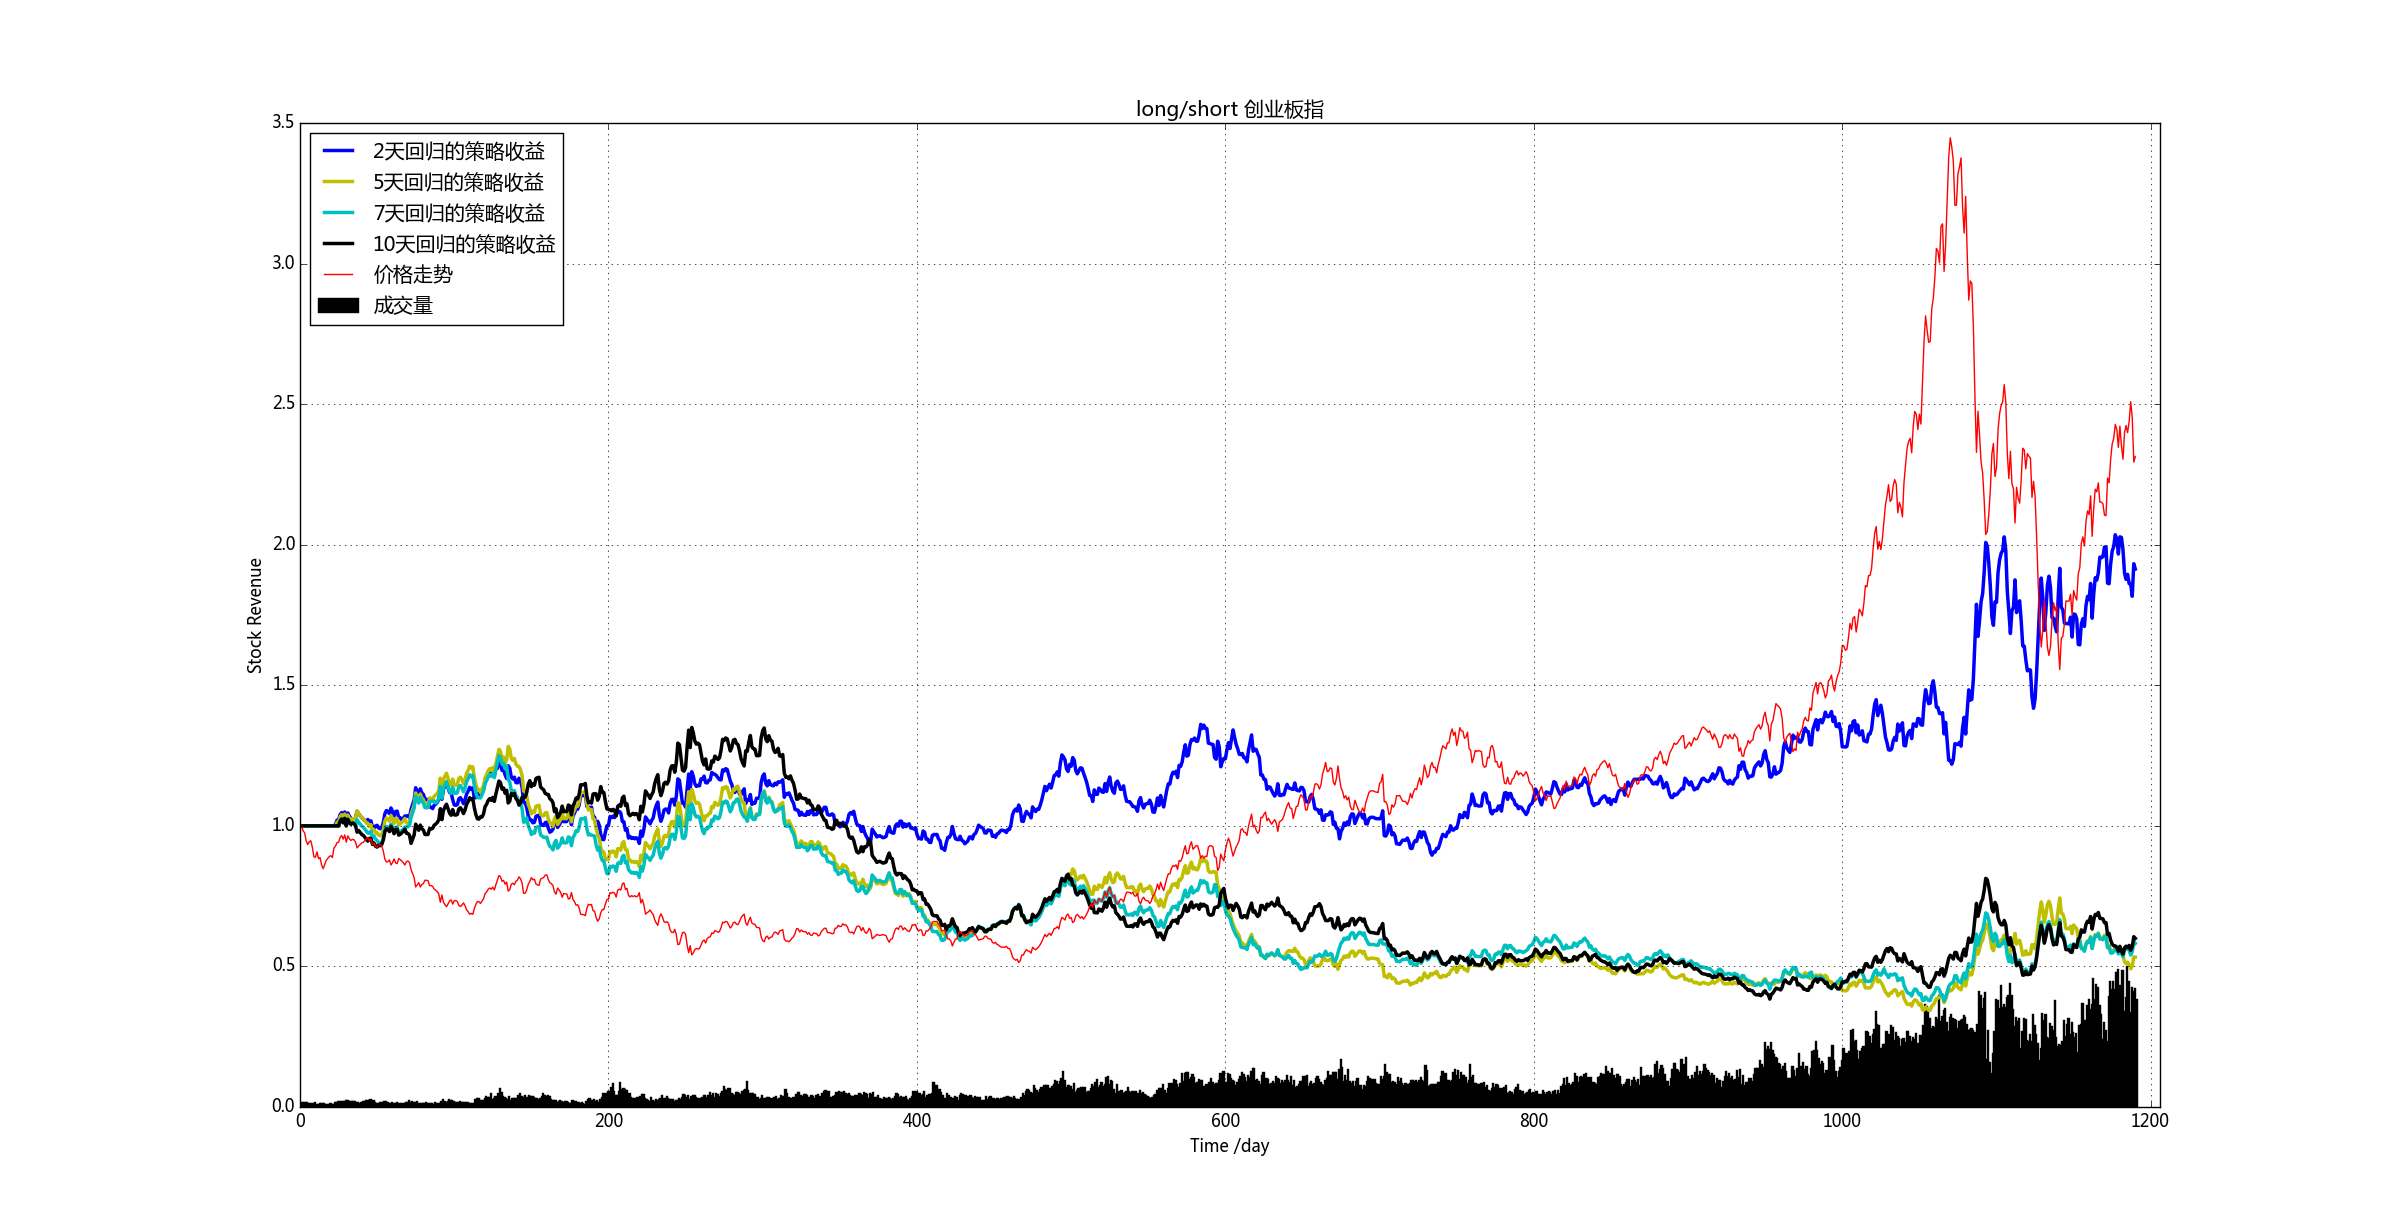
\includegraphics[width=1.0\textwidth]{img_r_7/cyb.png}
	\caption{创业板 long/short}
\end{figure}
\item long/hold 
\begin{figure}[H]
	\centering
	\includegraphics[width=1.0\textwidth]{img_r_7/cyb_1.png}
	\caption{创业板 long/hold }
\end{figure}
\end{enumerate}

\subsubsection{中证500}
\begin{enumerate}
\item long/short 
\begin{figure}[H]
	\centering
	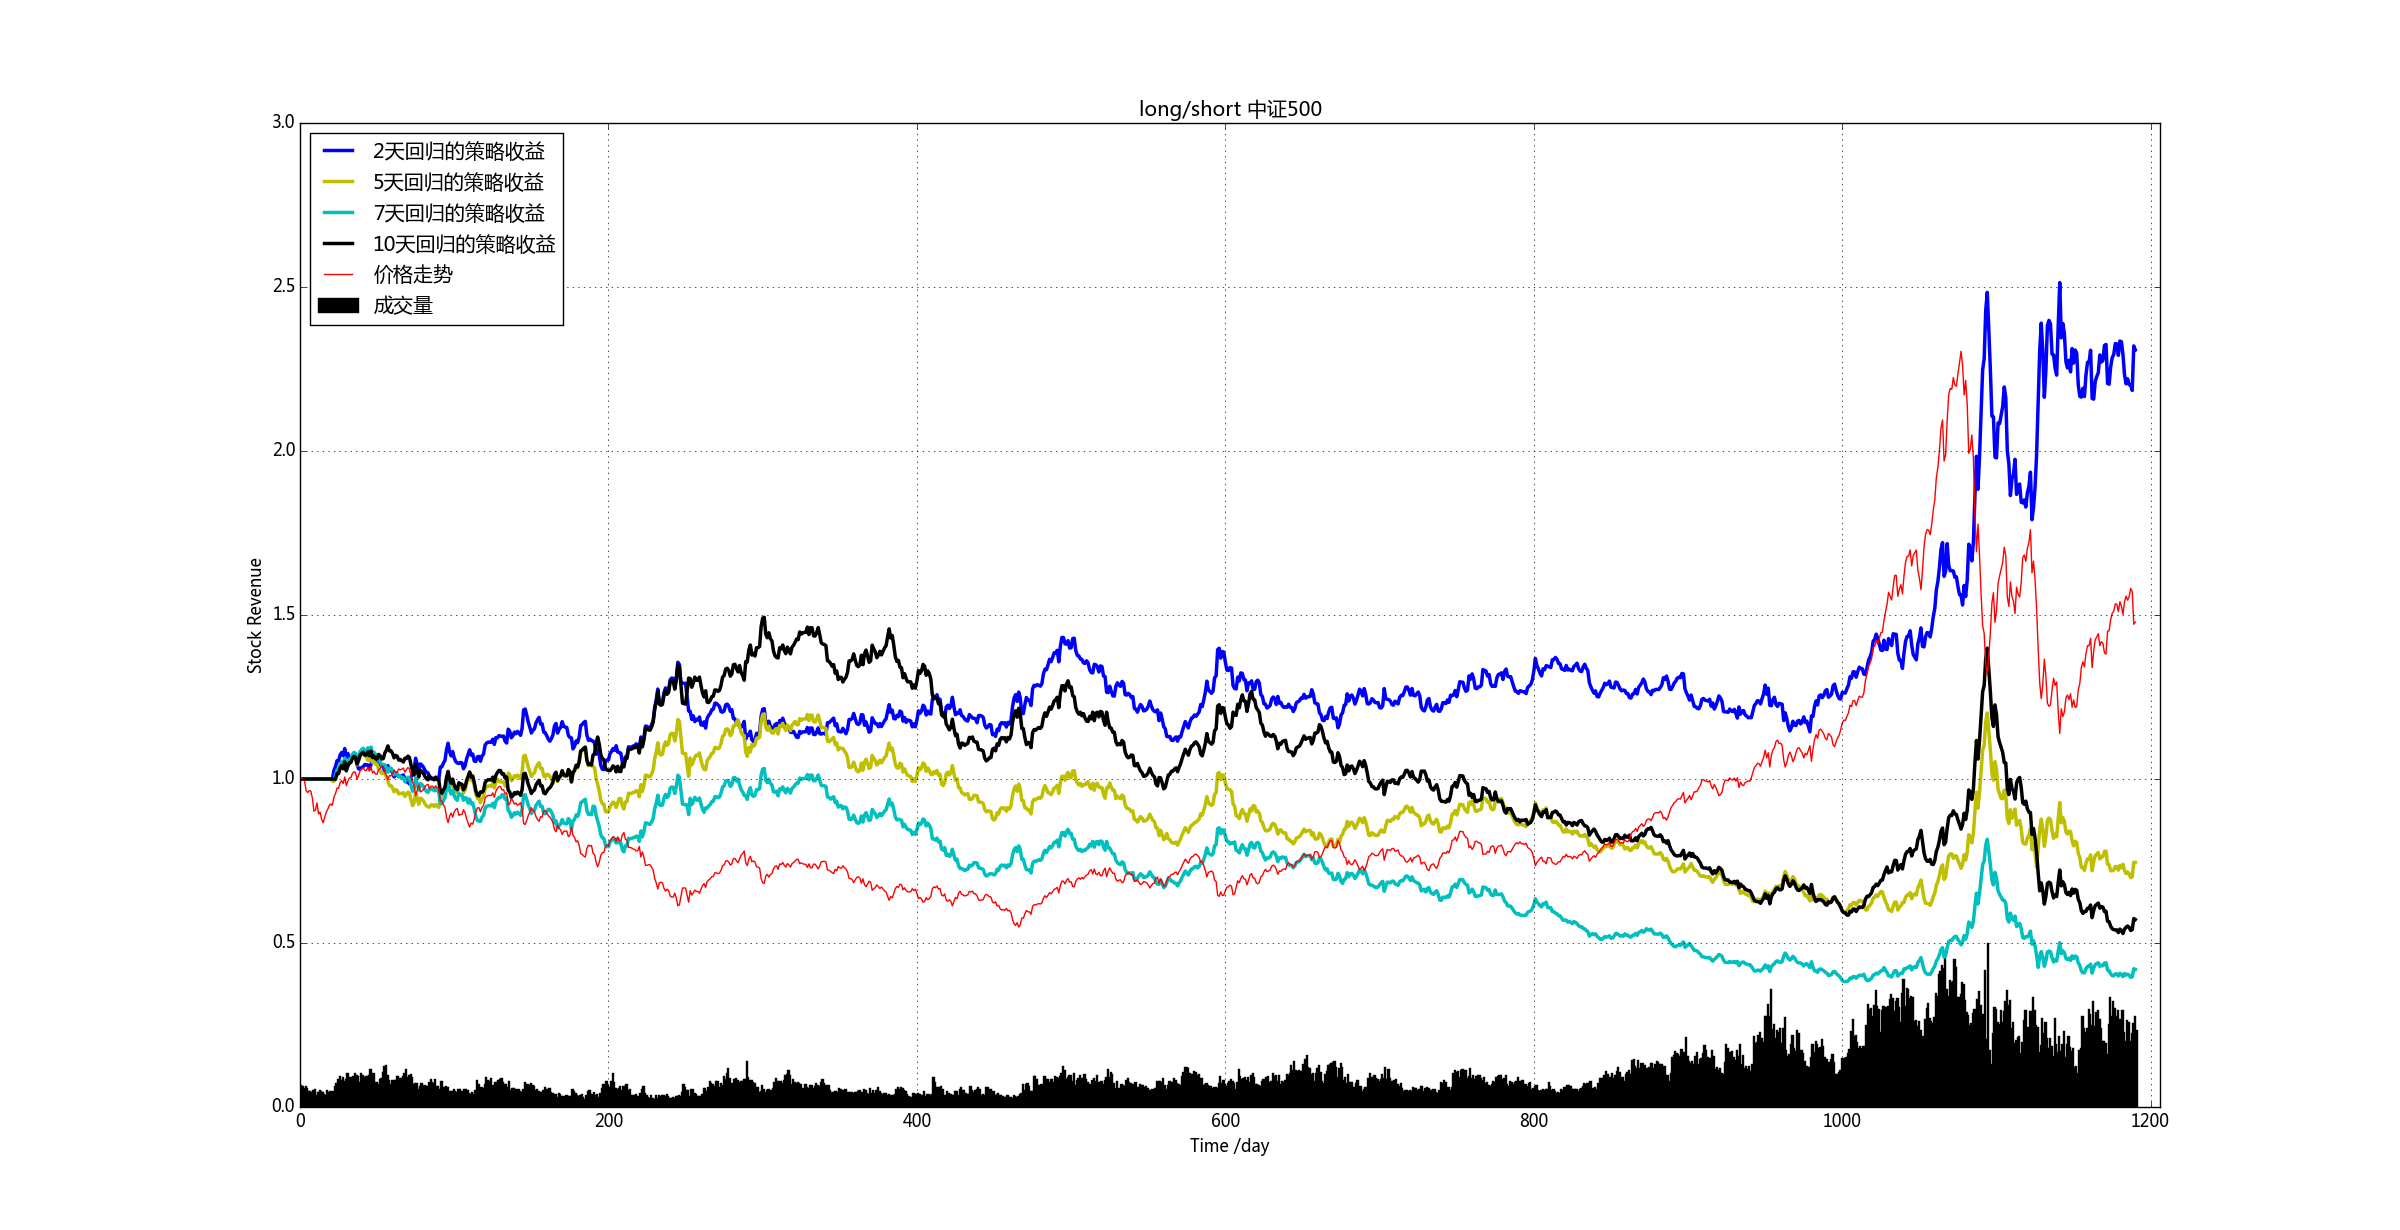
\includegraphics[width=1.0\textwidth]{img_r_7/zz500.png}
	\caption{中证500 long/short }
\end{figure}
\item long/hold 
\begin{figure}[H]
	\centering
	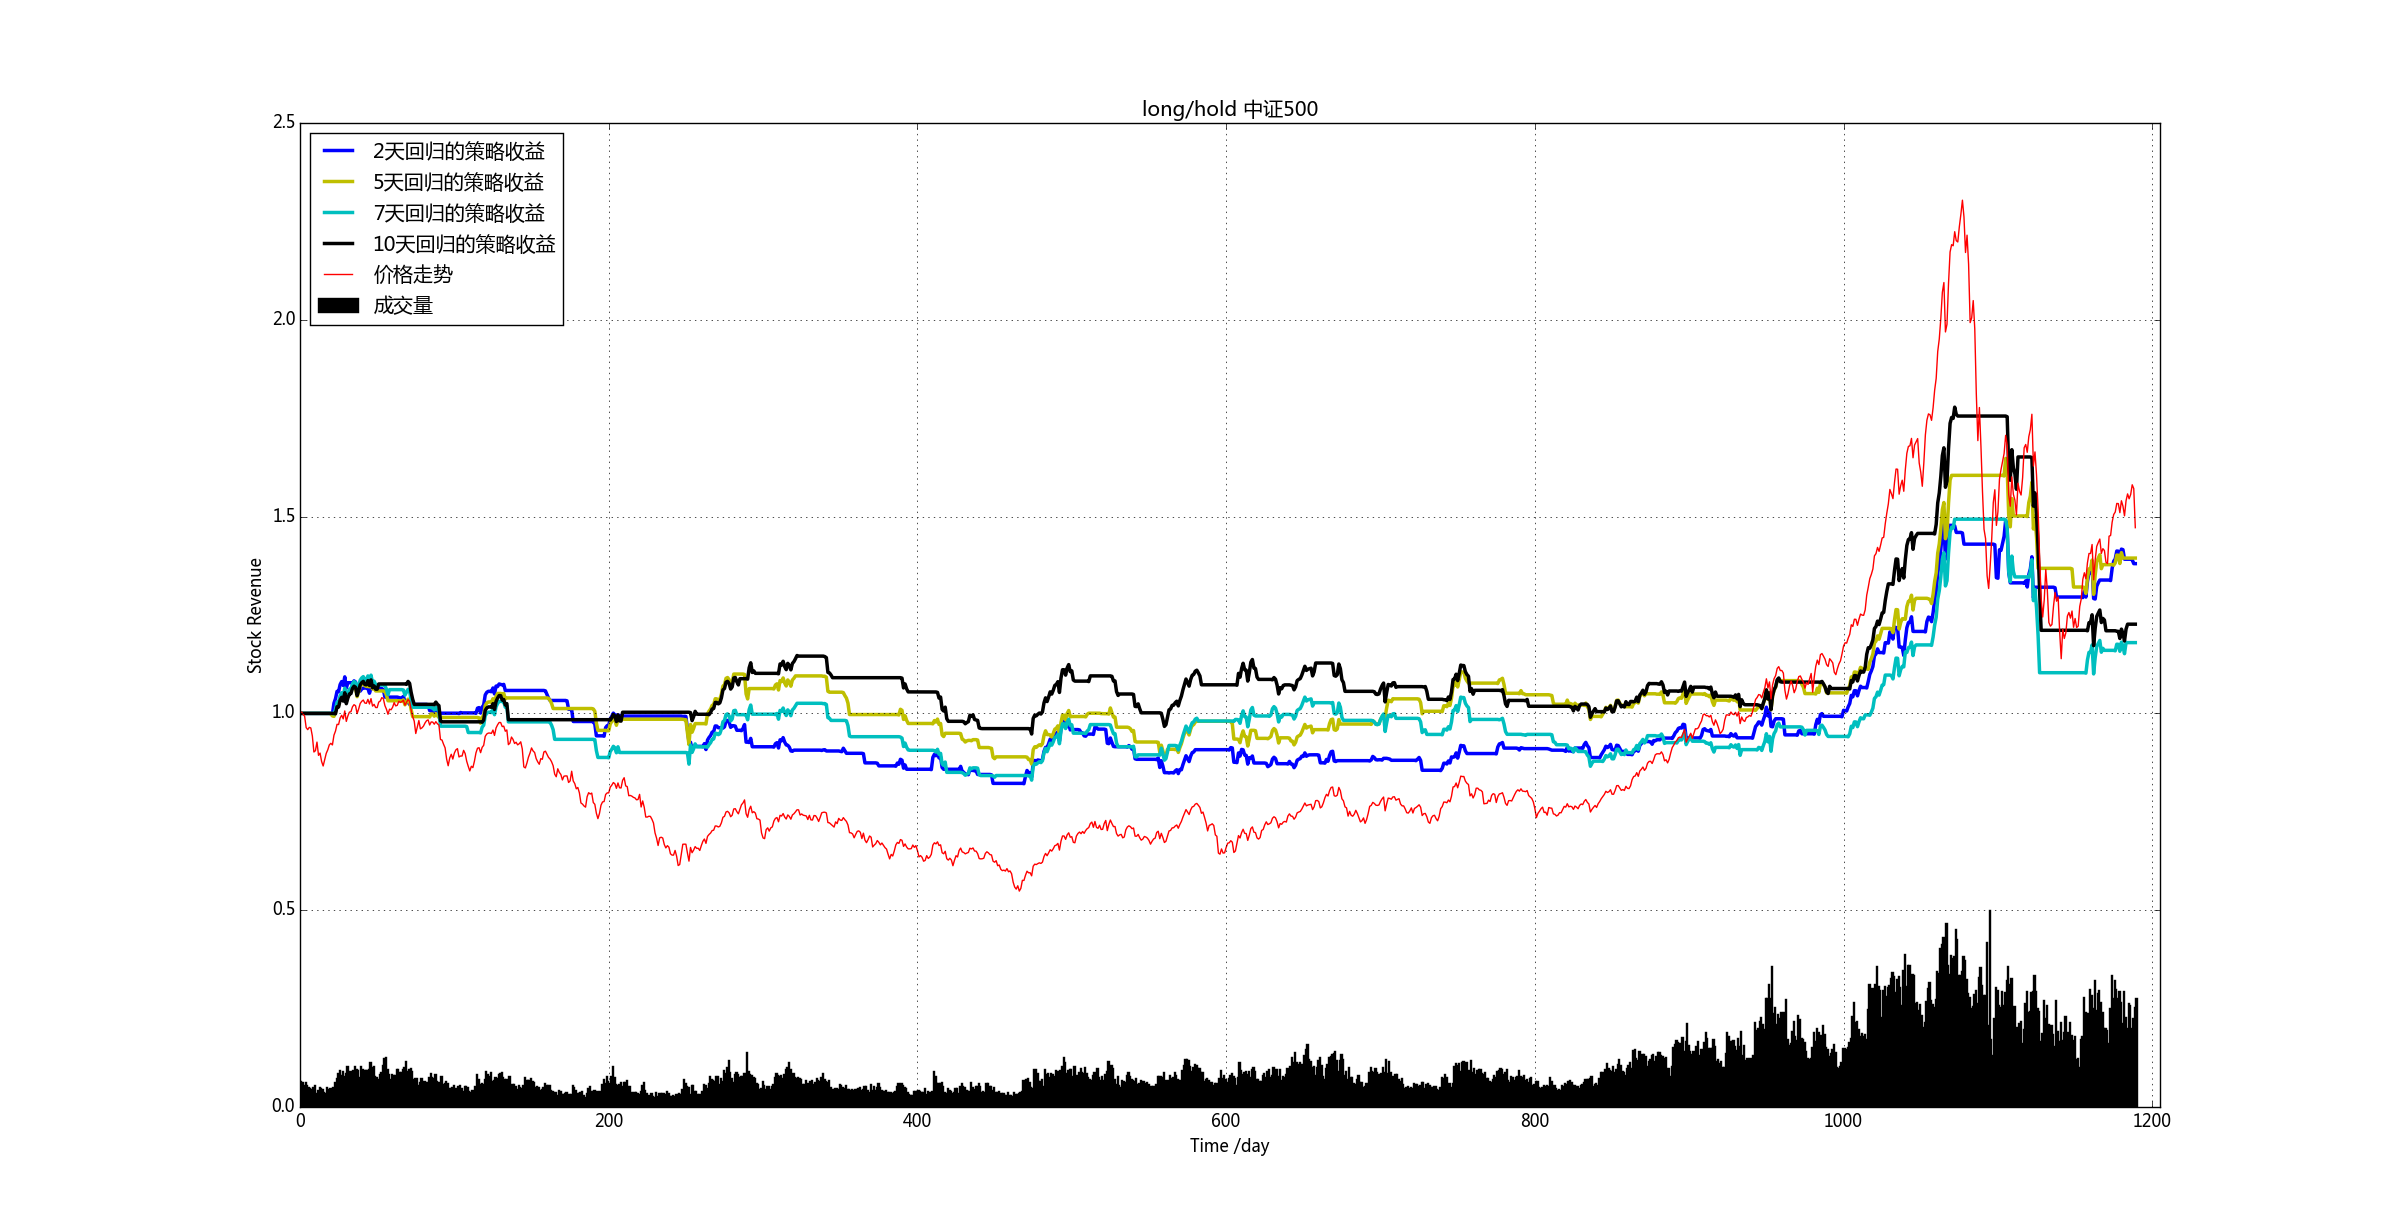
\includegraphics[width=1.0\textwidth]{img_r_7/zz500_1.png}
	\caption{中证500 long/hold}
\end{figure}
\end{enumerate}


\subsection{价格和成交量10日MA}
\subsubsection{上证50}

\begin{enumerate}
\item long/short 
\begin{figure}[H]
	\centering
	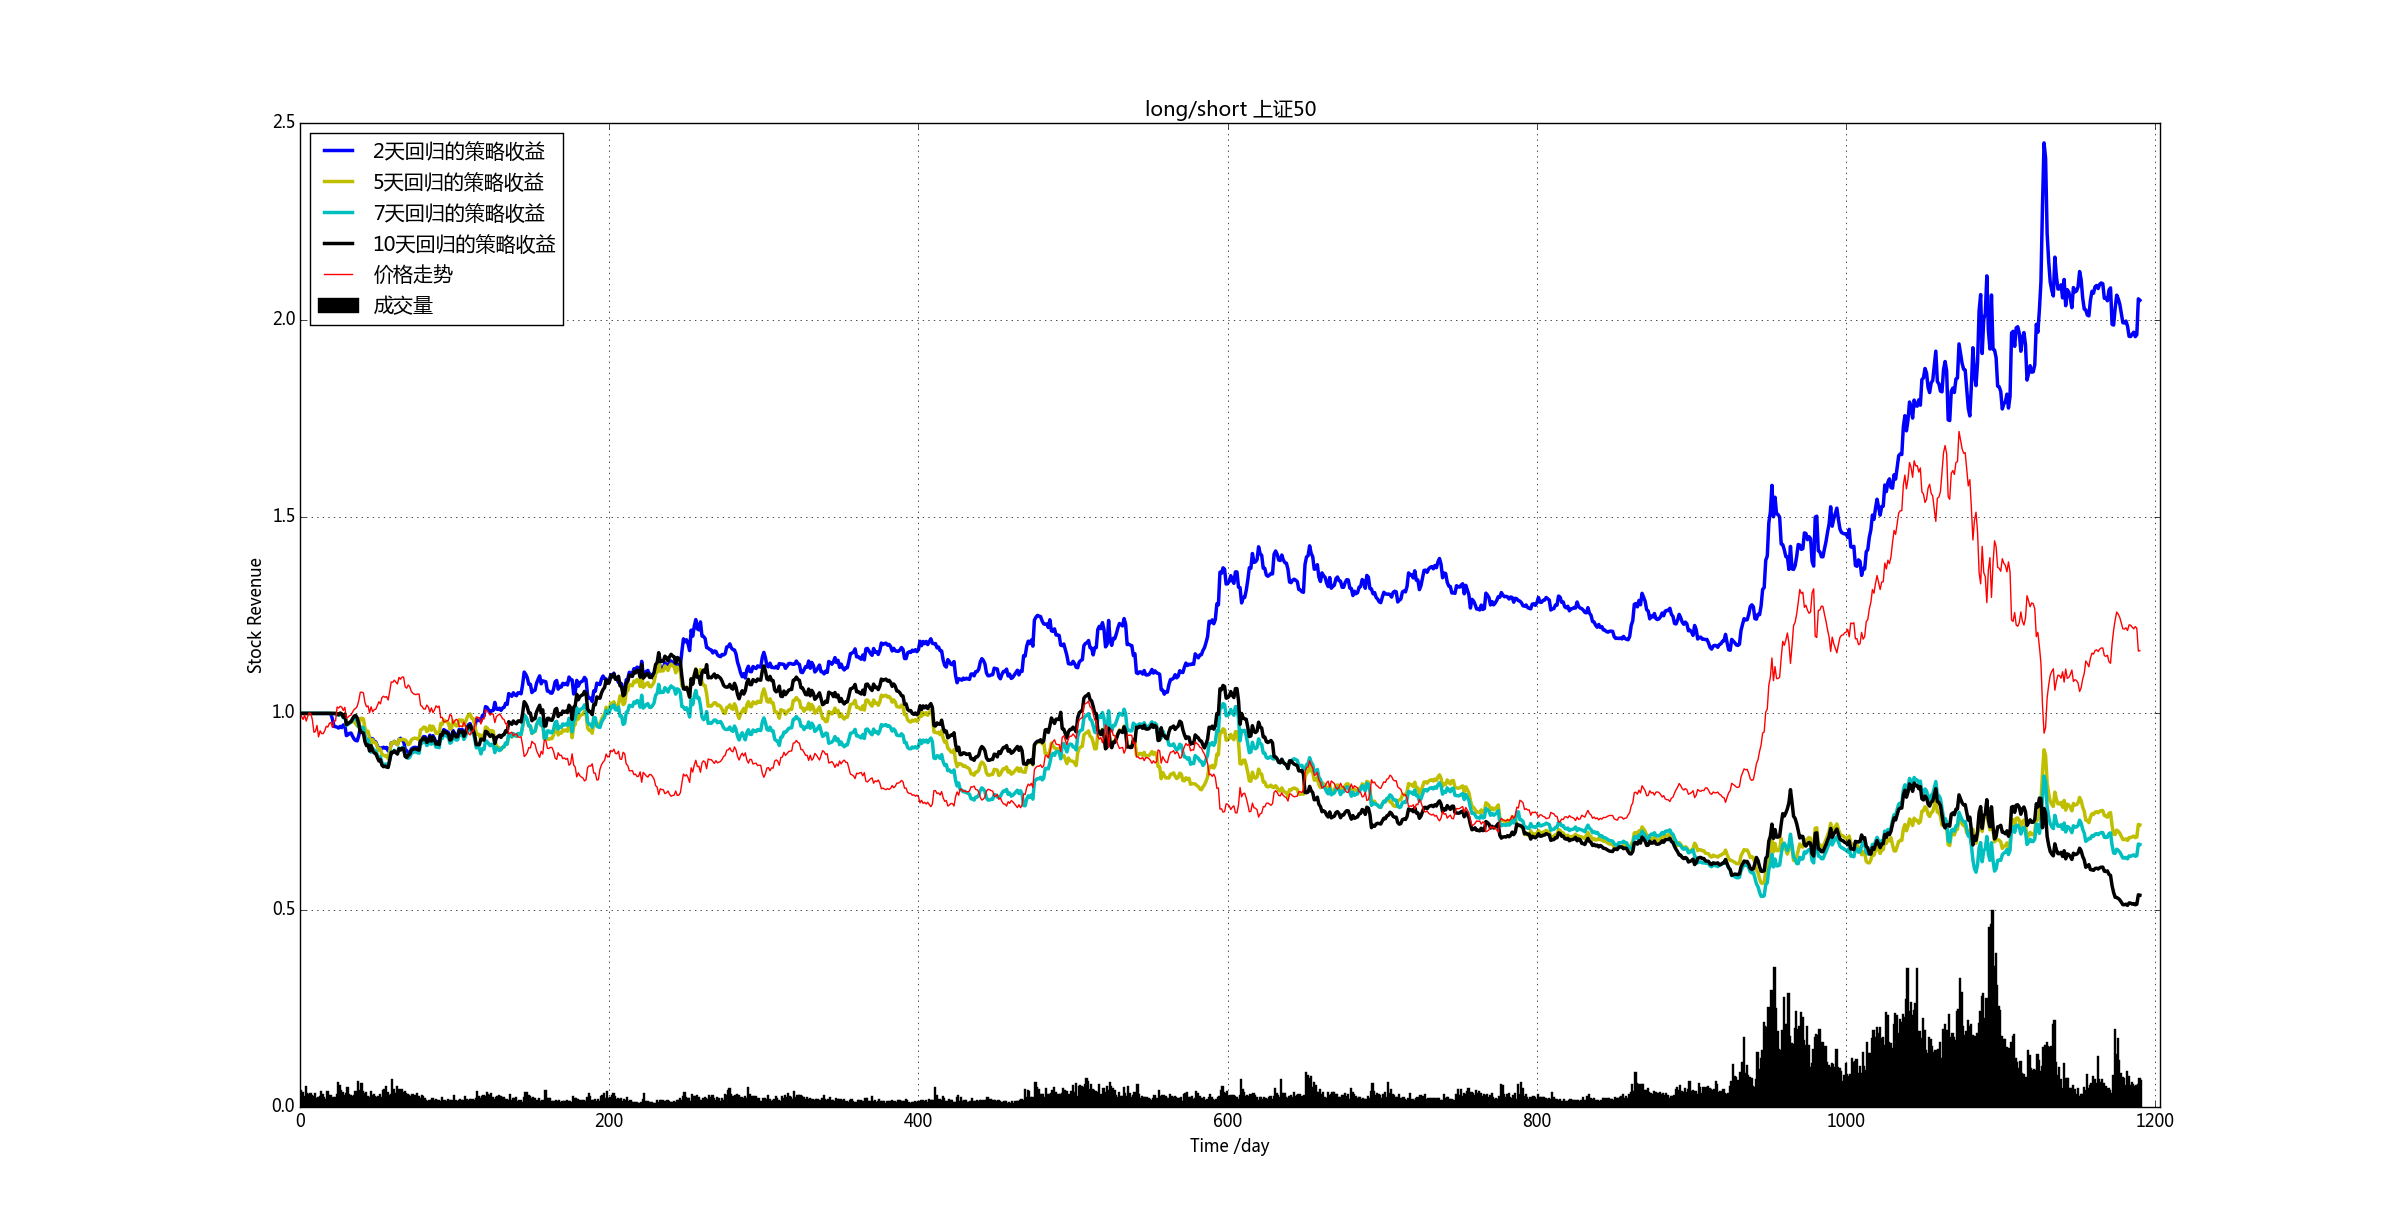
\includegraphics[width=1.0\textwidth]{img_r_10/sz50.png}
	\caption{上证50 long/short}
\end{figure}

\item long/hold 
\begin{figure}[H]
	\centering
	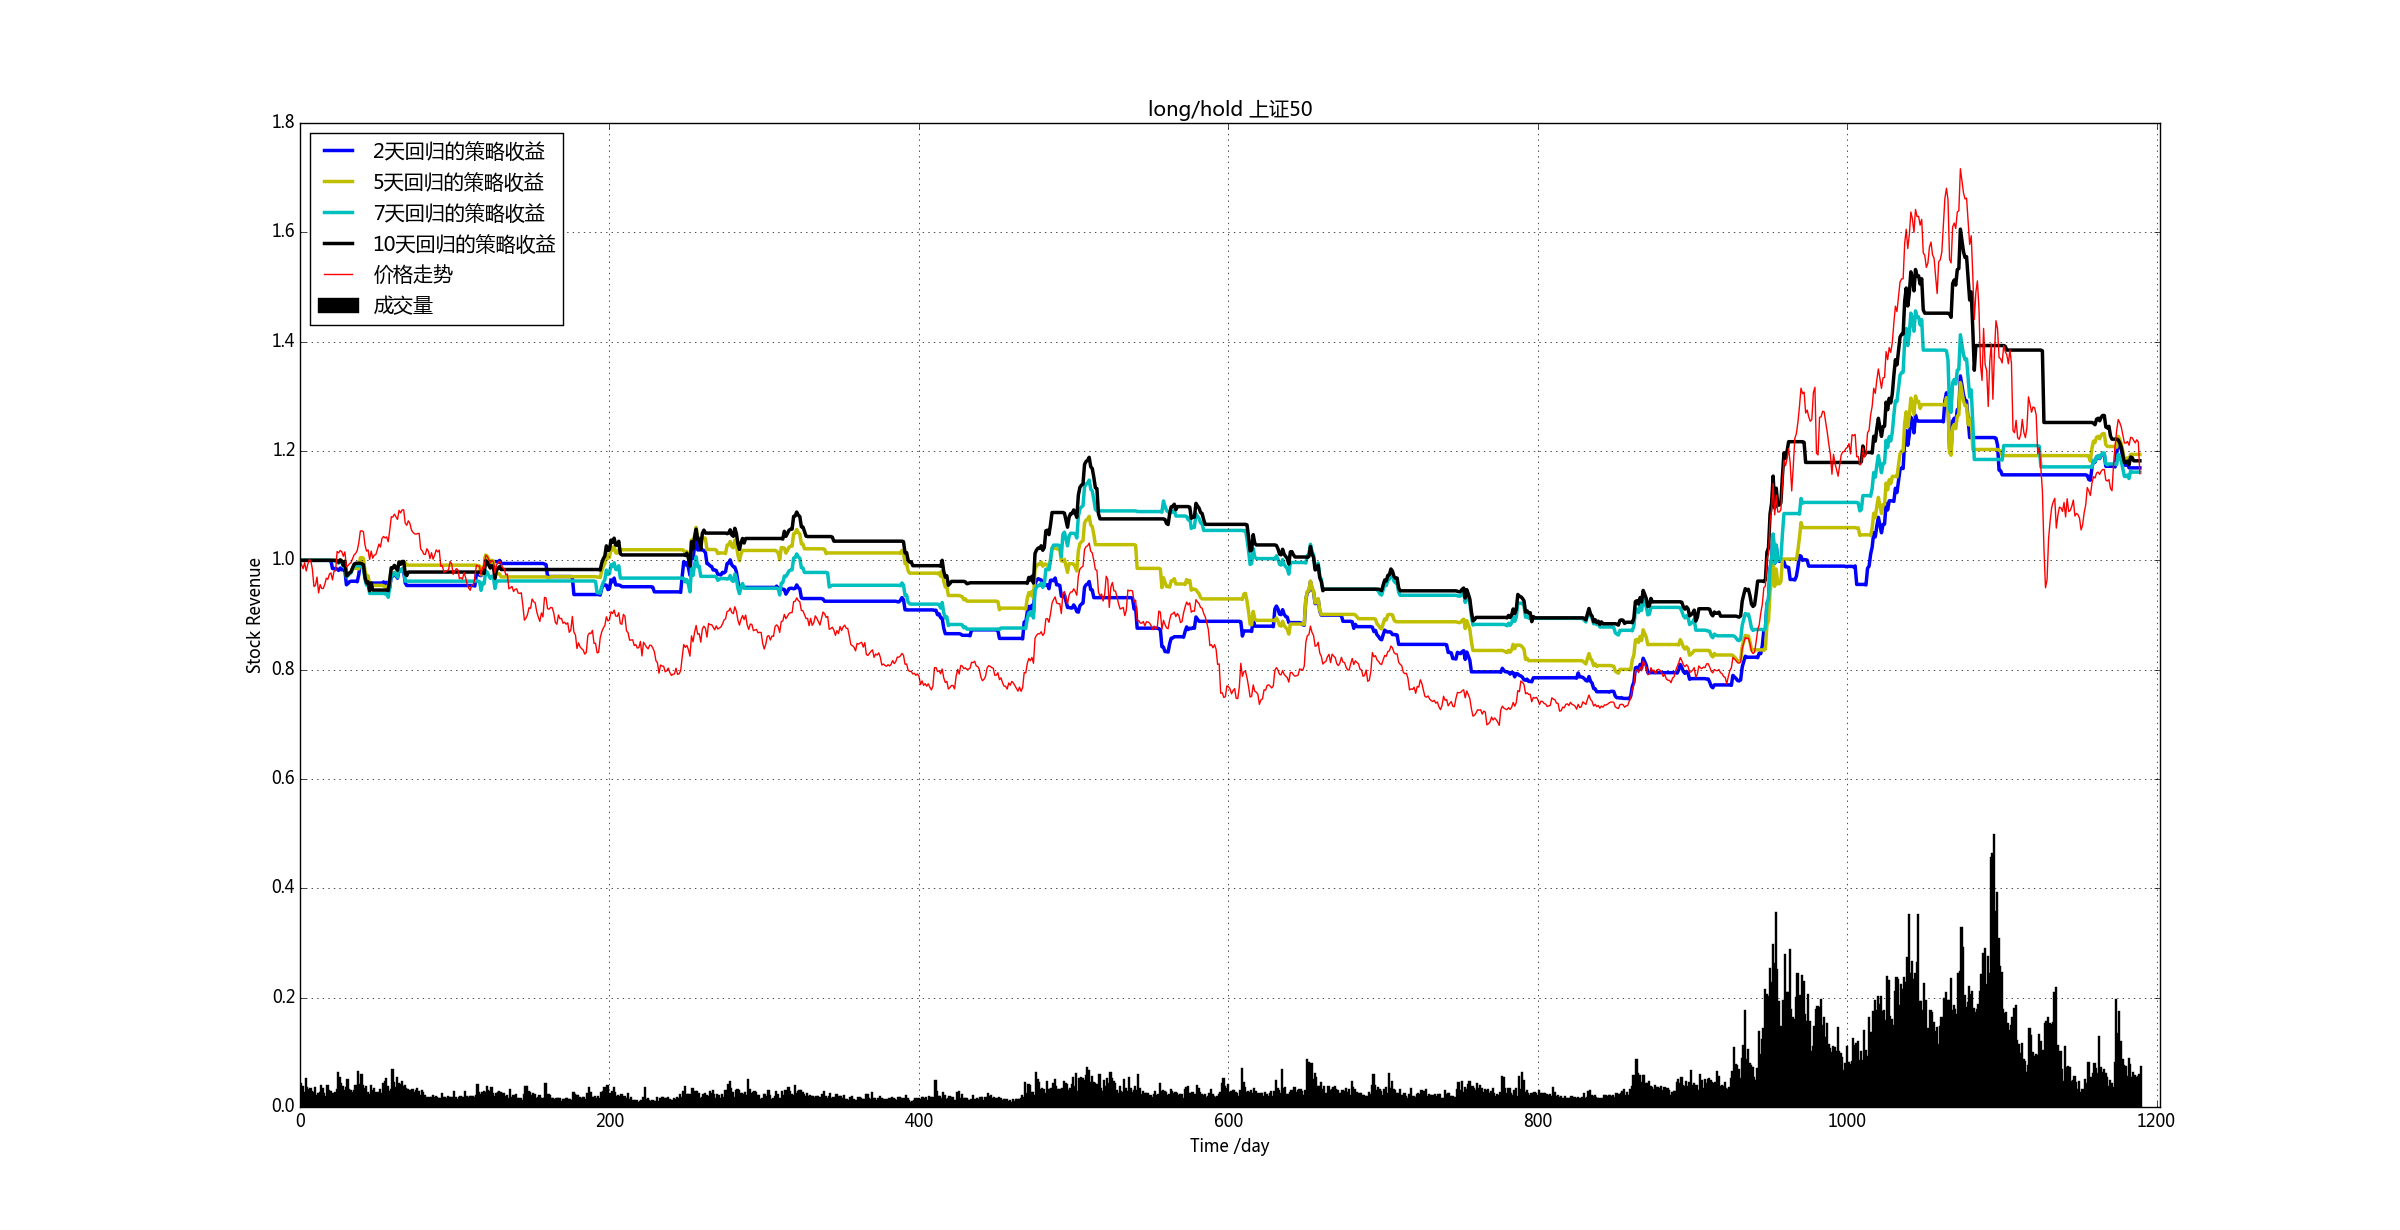
\includegraphics[width=1.0\textwidth]{img_r_10/sz50_1.png}
	\caption{上证50 long/hold}
\end{figure}
\end{enumerate}

\subsubsection{上证综指}

\begin{enumerate}
\item long/short 
\begin{figure}[H]
	\centering
	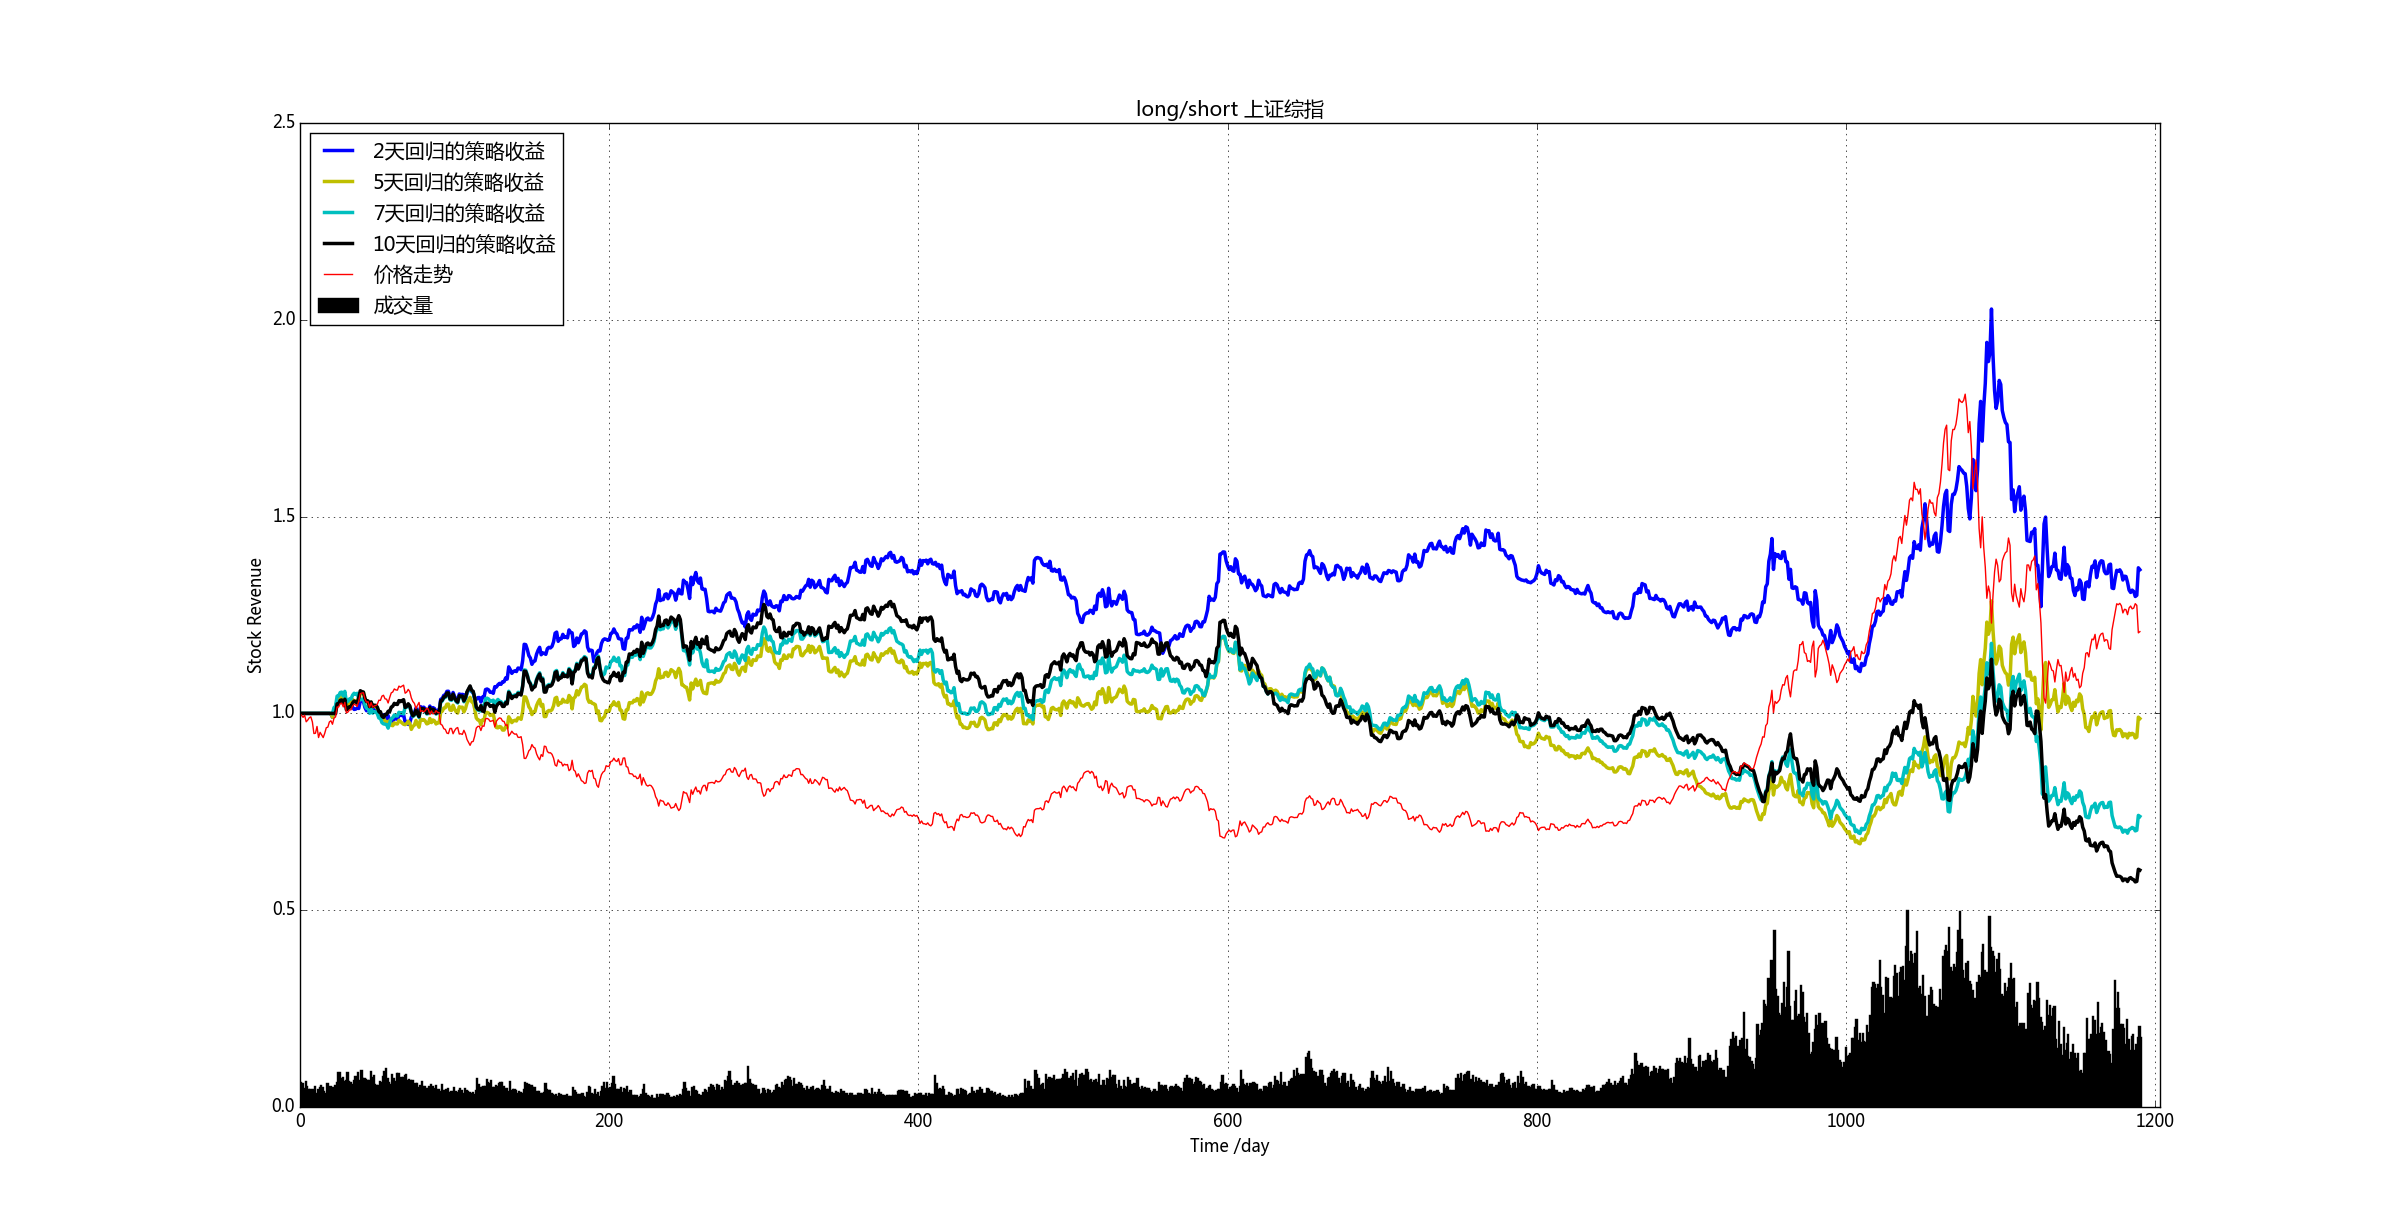
\includegraphics[width=1.0\textwidth]{img_r_10/szzz.png}
	\caption{上证综指 long/short}
\end{figure}
\item long/hold 
\begin{figure}[H]
	\centering
	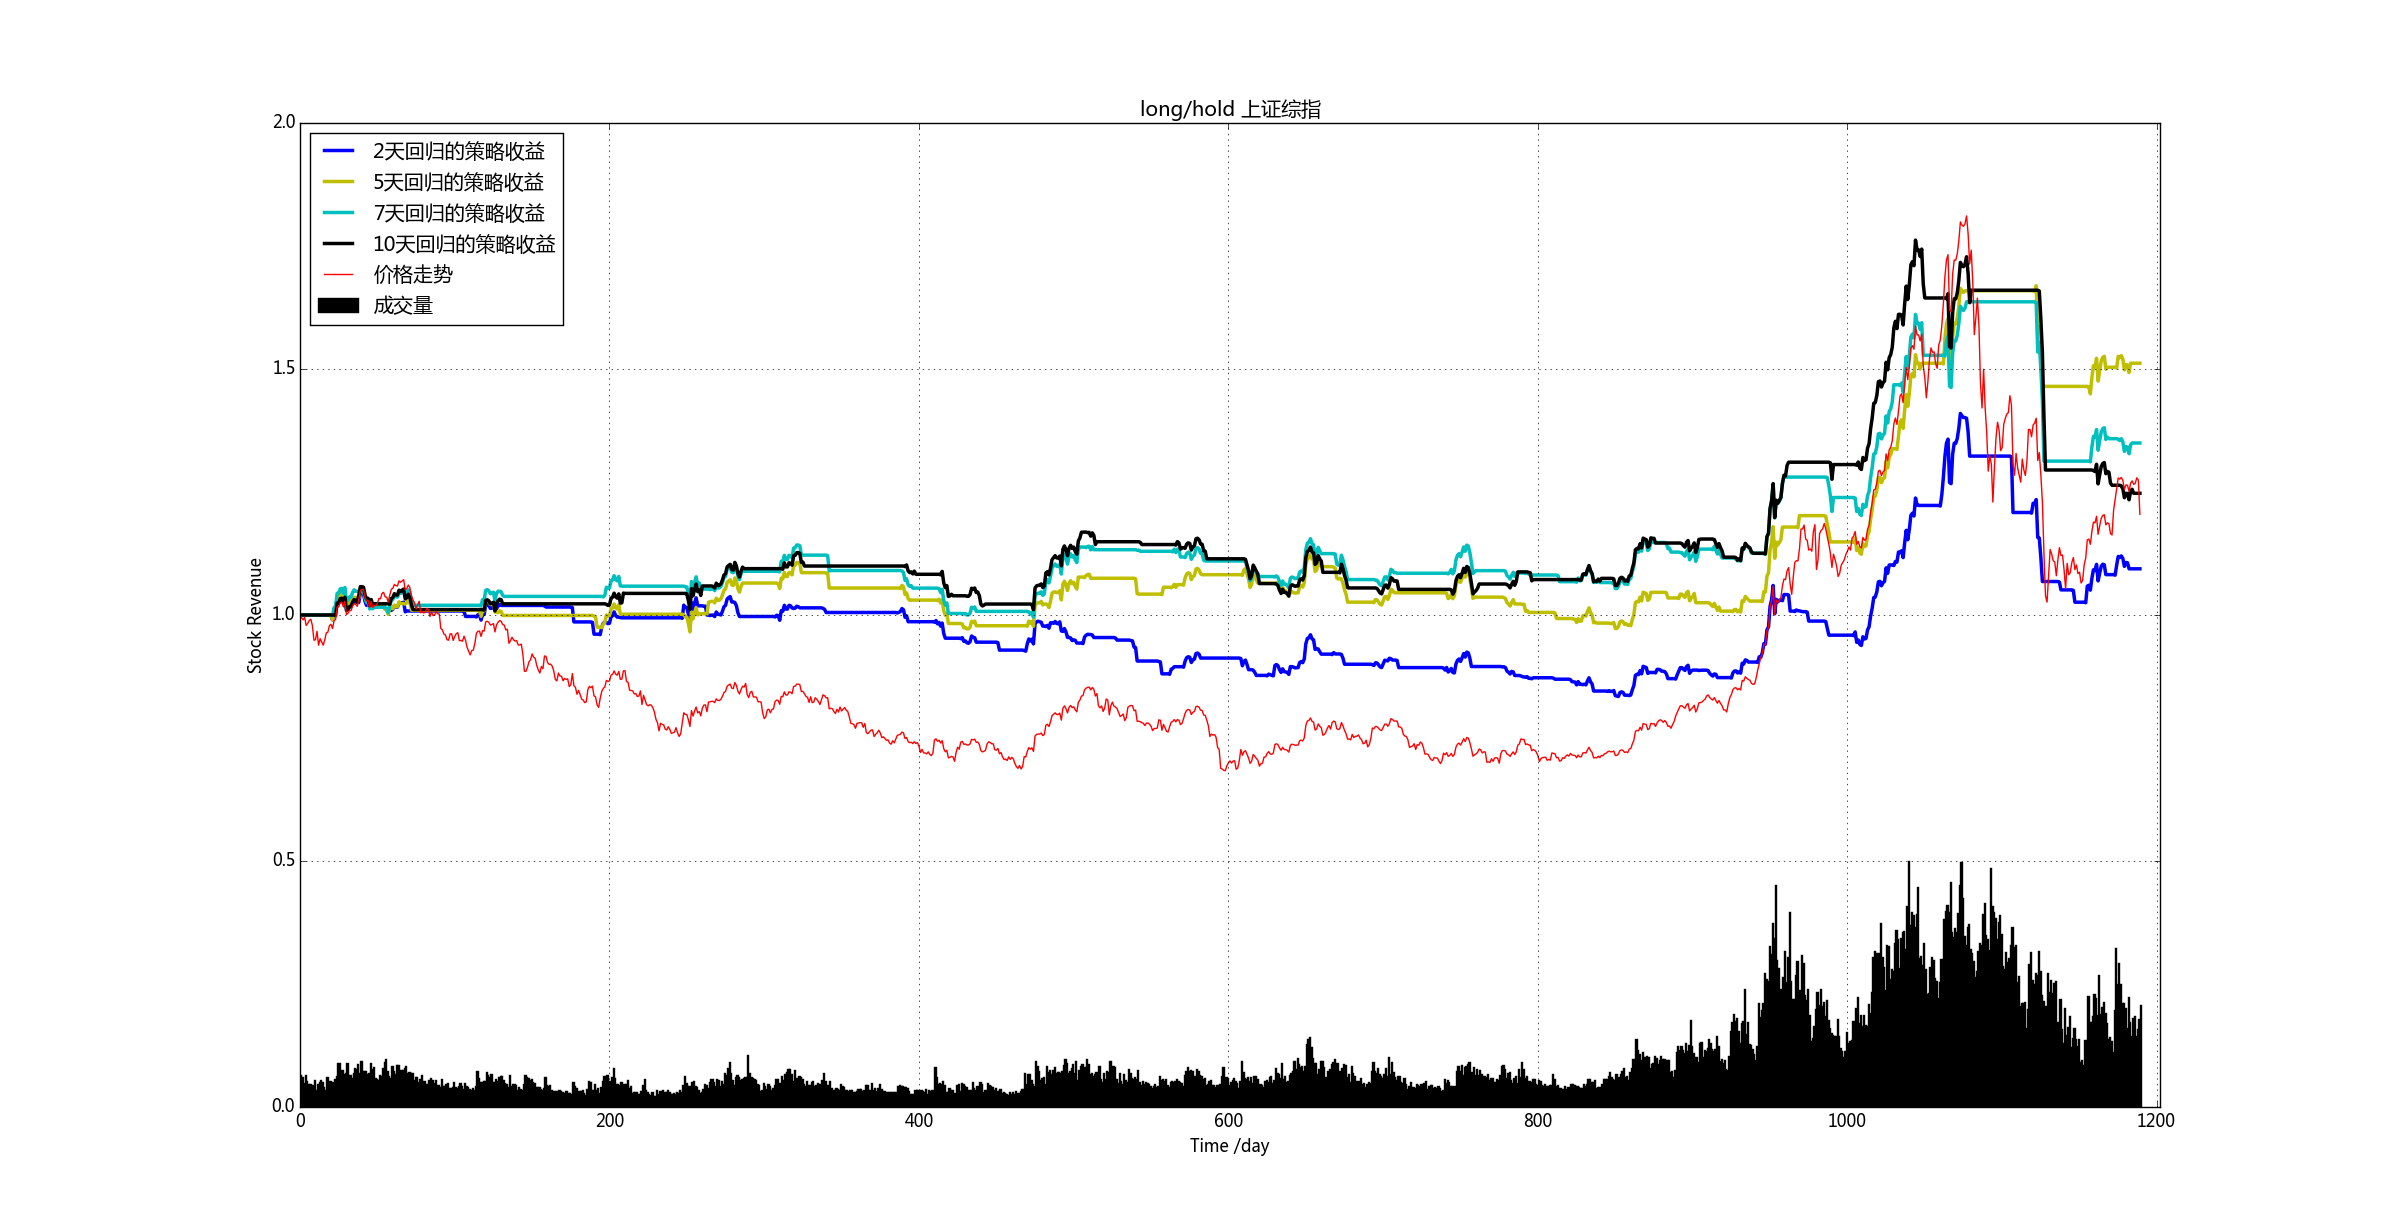
\includegraphics[width=1.0\textwidth]{img_r_10/szzz_1.png}
	\caption{上证综指 long/hold}
\end{figure}
\end{enumerate}

\subsubsection{沪深300}
\begin{enumerate}
\item long/short 
\begin{figure}[H]
	\centering
	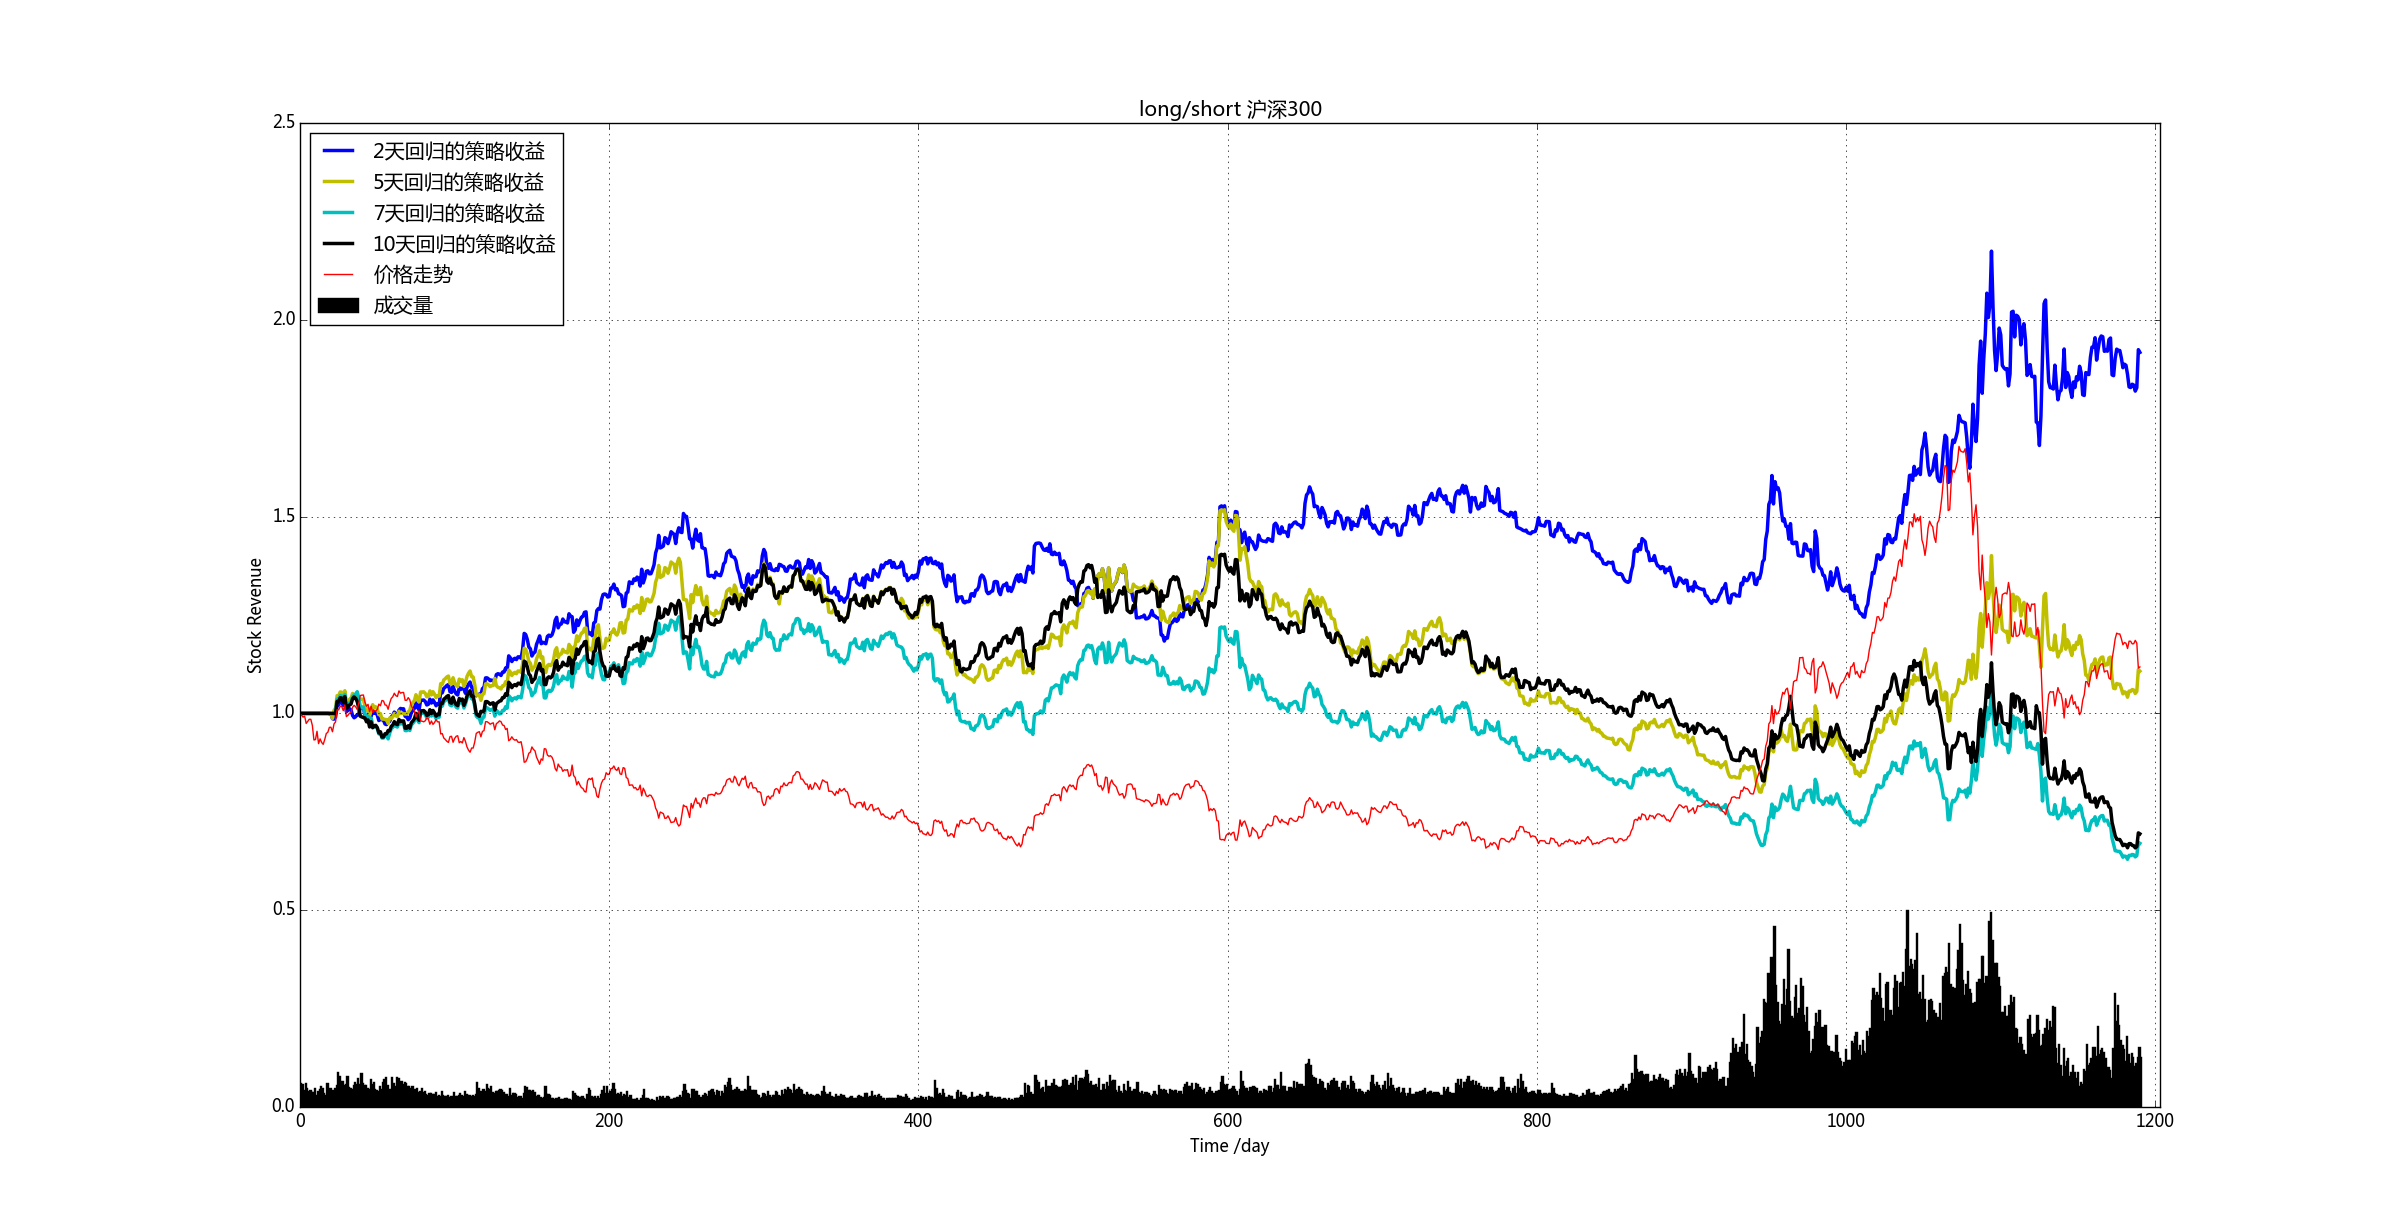
\includegraphics[width=1.0\textwidth]{img_r_10/hs300.png}
	\caption{沪深300 long/short }
\end{figure}
\item long/hold 
\begin{figure}[H]
	\centering
	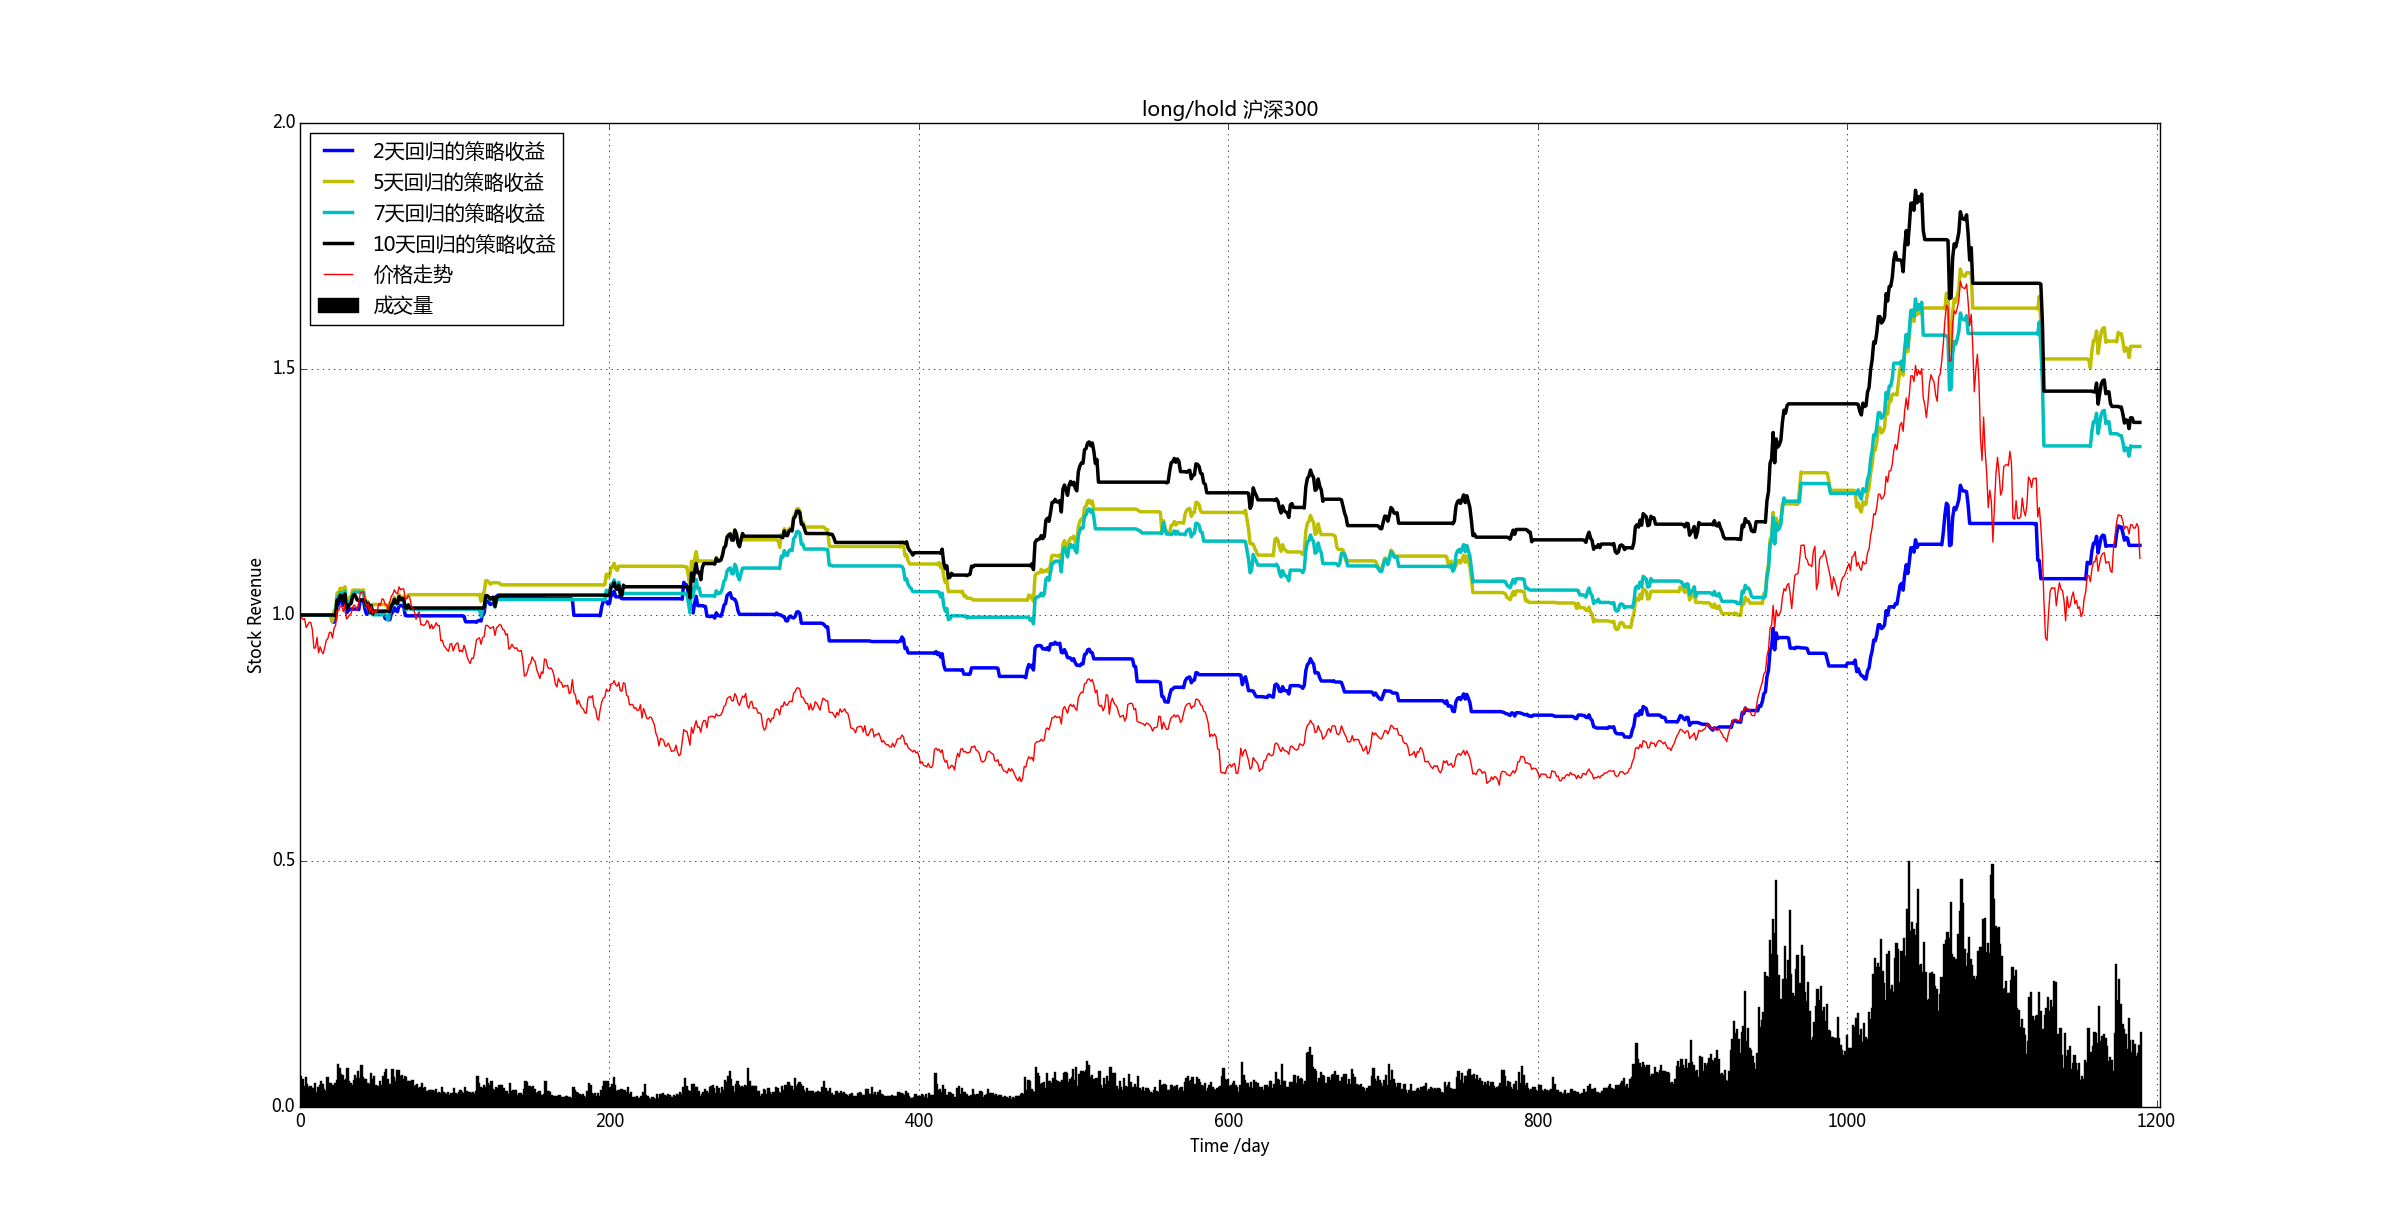
\includegraphics[width=1.0\textwidth]{img_r_10/hs300_1.png}
	\caption{沪深300 long/hold }
\end{figure}
\end{enumerate}

\subsubsection{创业板}
\begin{enumerate}
\item long/short 
\begin{figure}[H]
	\centering
	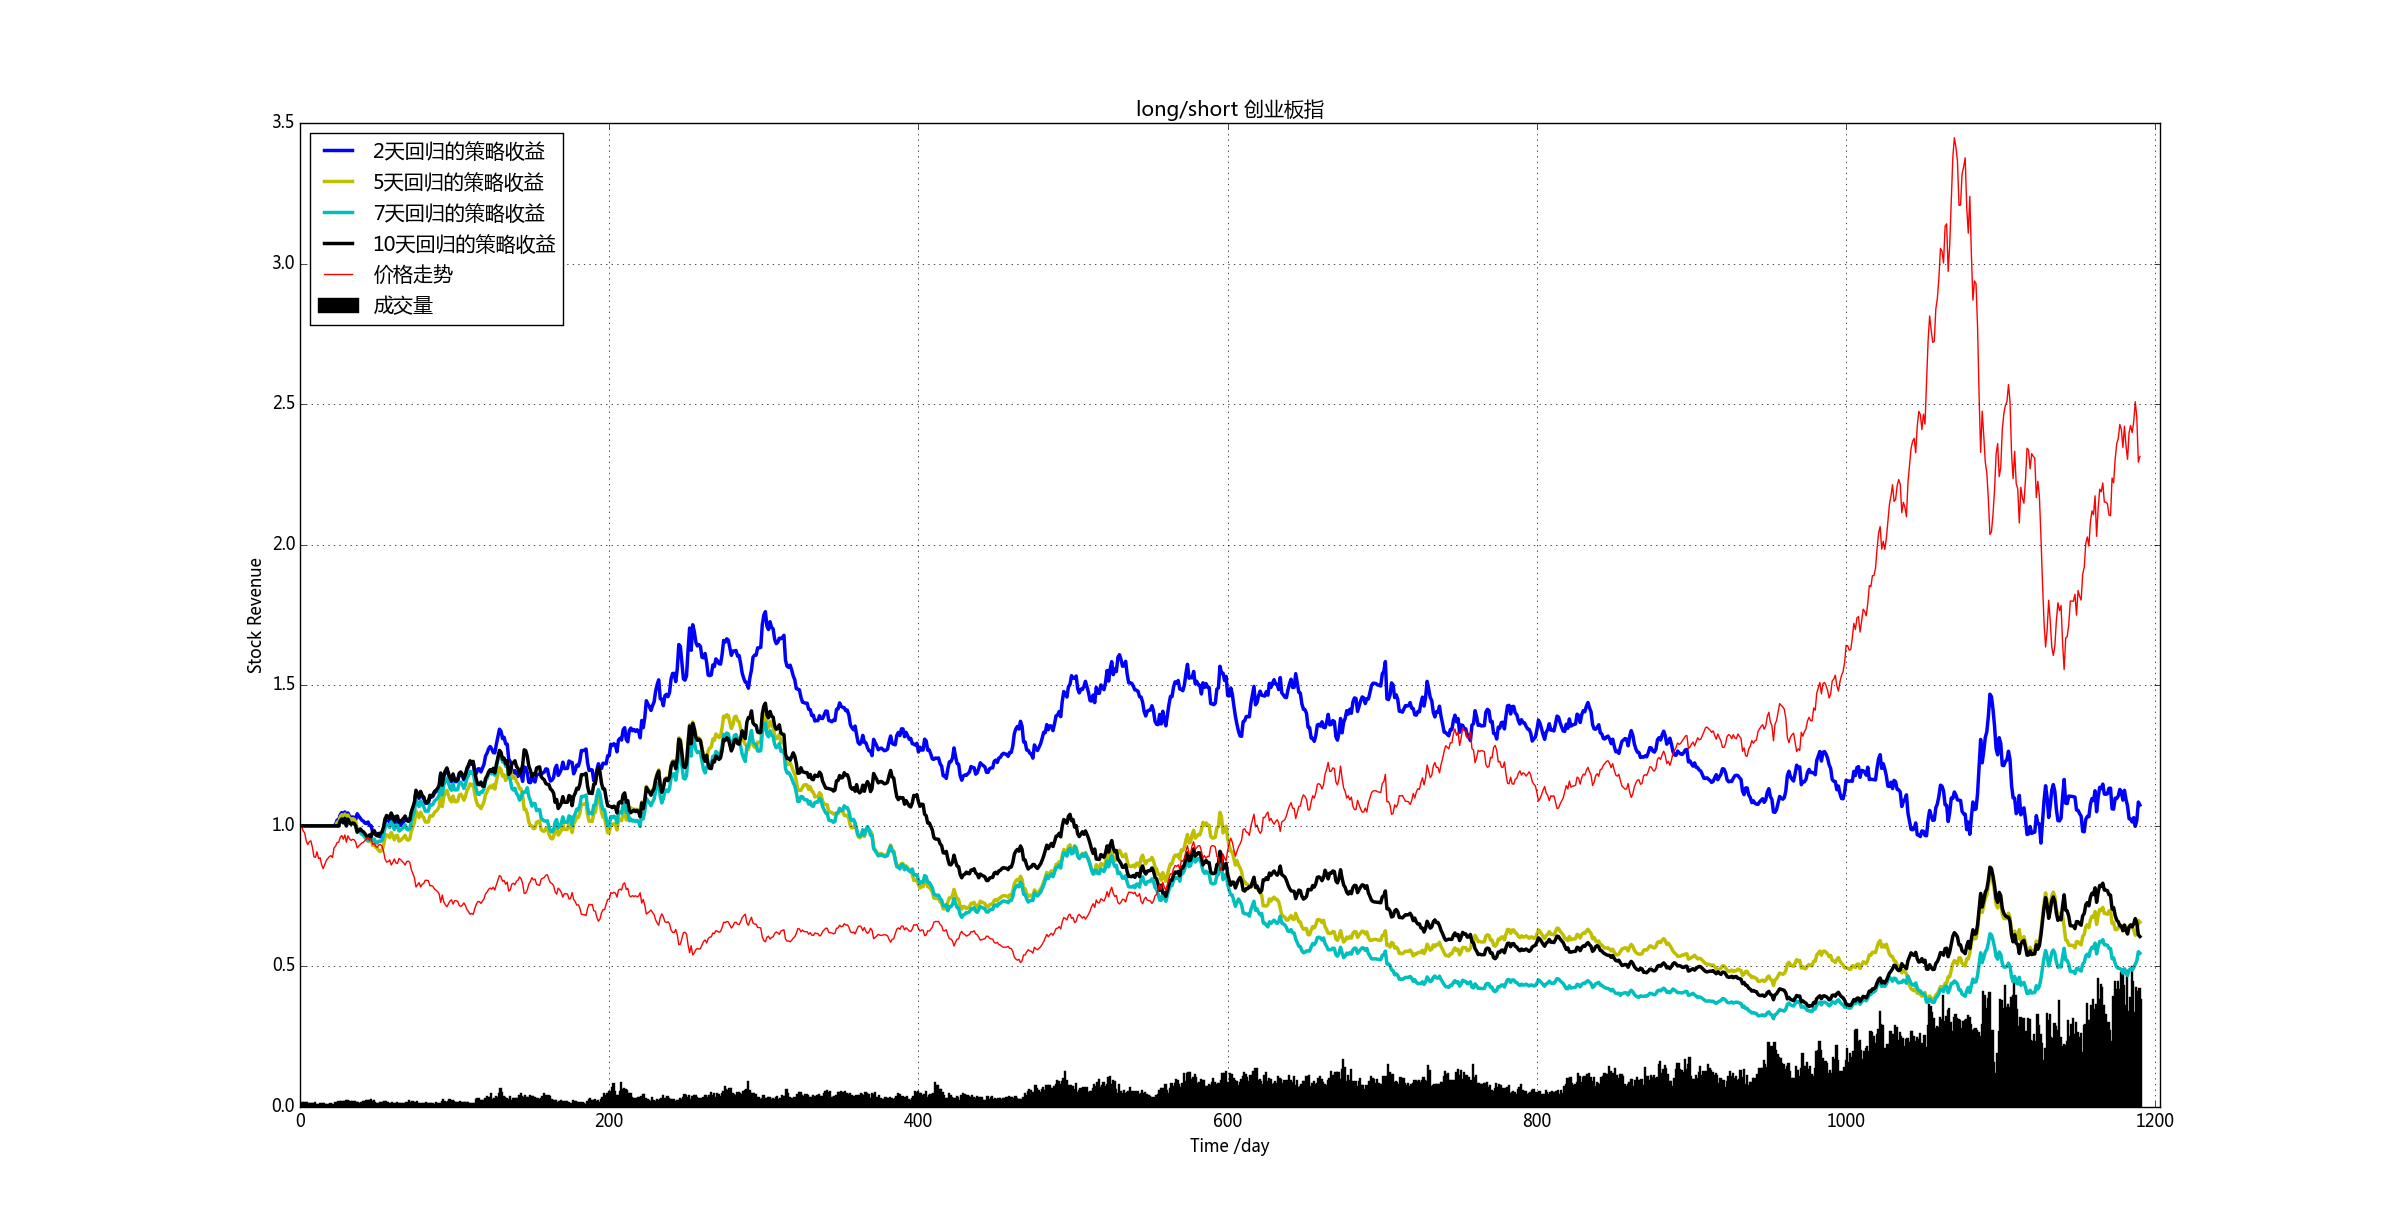
\includegraphics[width=1.0\textwidth]{img_r_10/cyb.png}
	\caption{创业板 long/short}
\end{figure}
\item long/hold 
\begin{figure}[H]
	\centering
	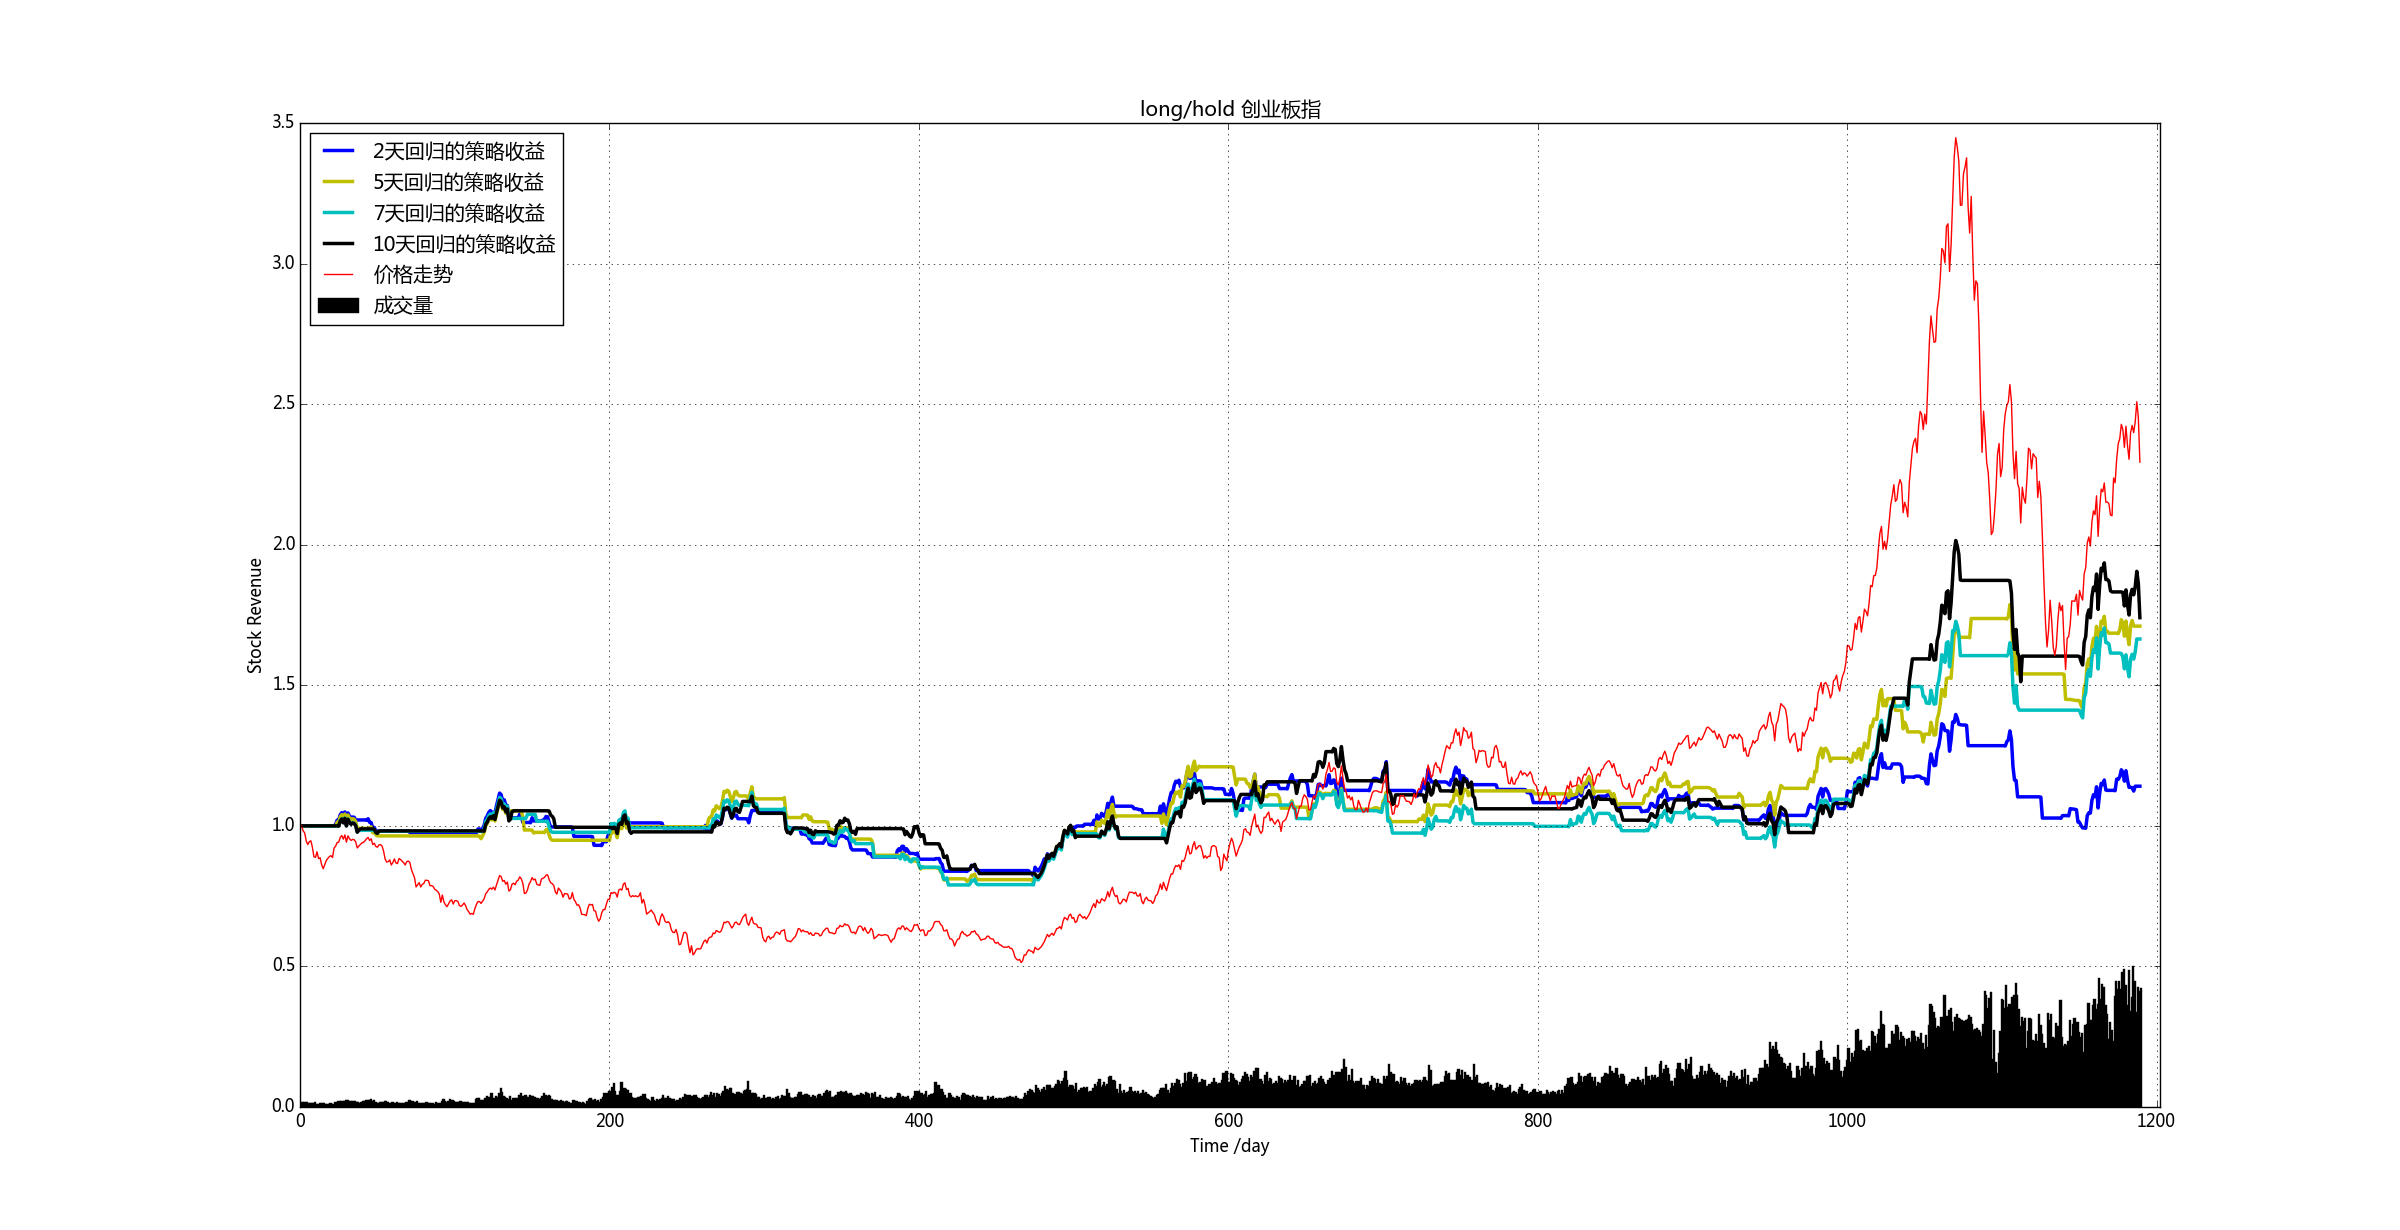
\includegraphics[width=1.0\textwidth]{img_r_10/cyb_1.png}
	\caption{创业板 long/hold }
\end{figure}
\end{enumerate}

\subsubsection{中证500}
\begin{enumerate}
\item long/short 
\begin{figure}[H]
	\centering
	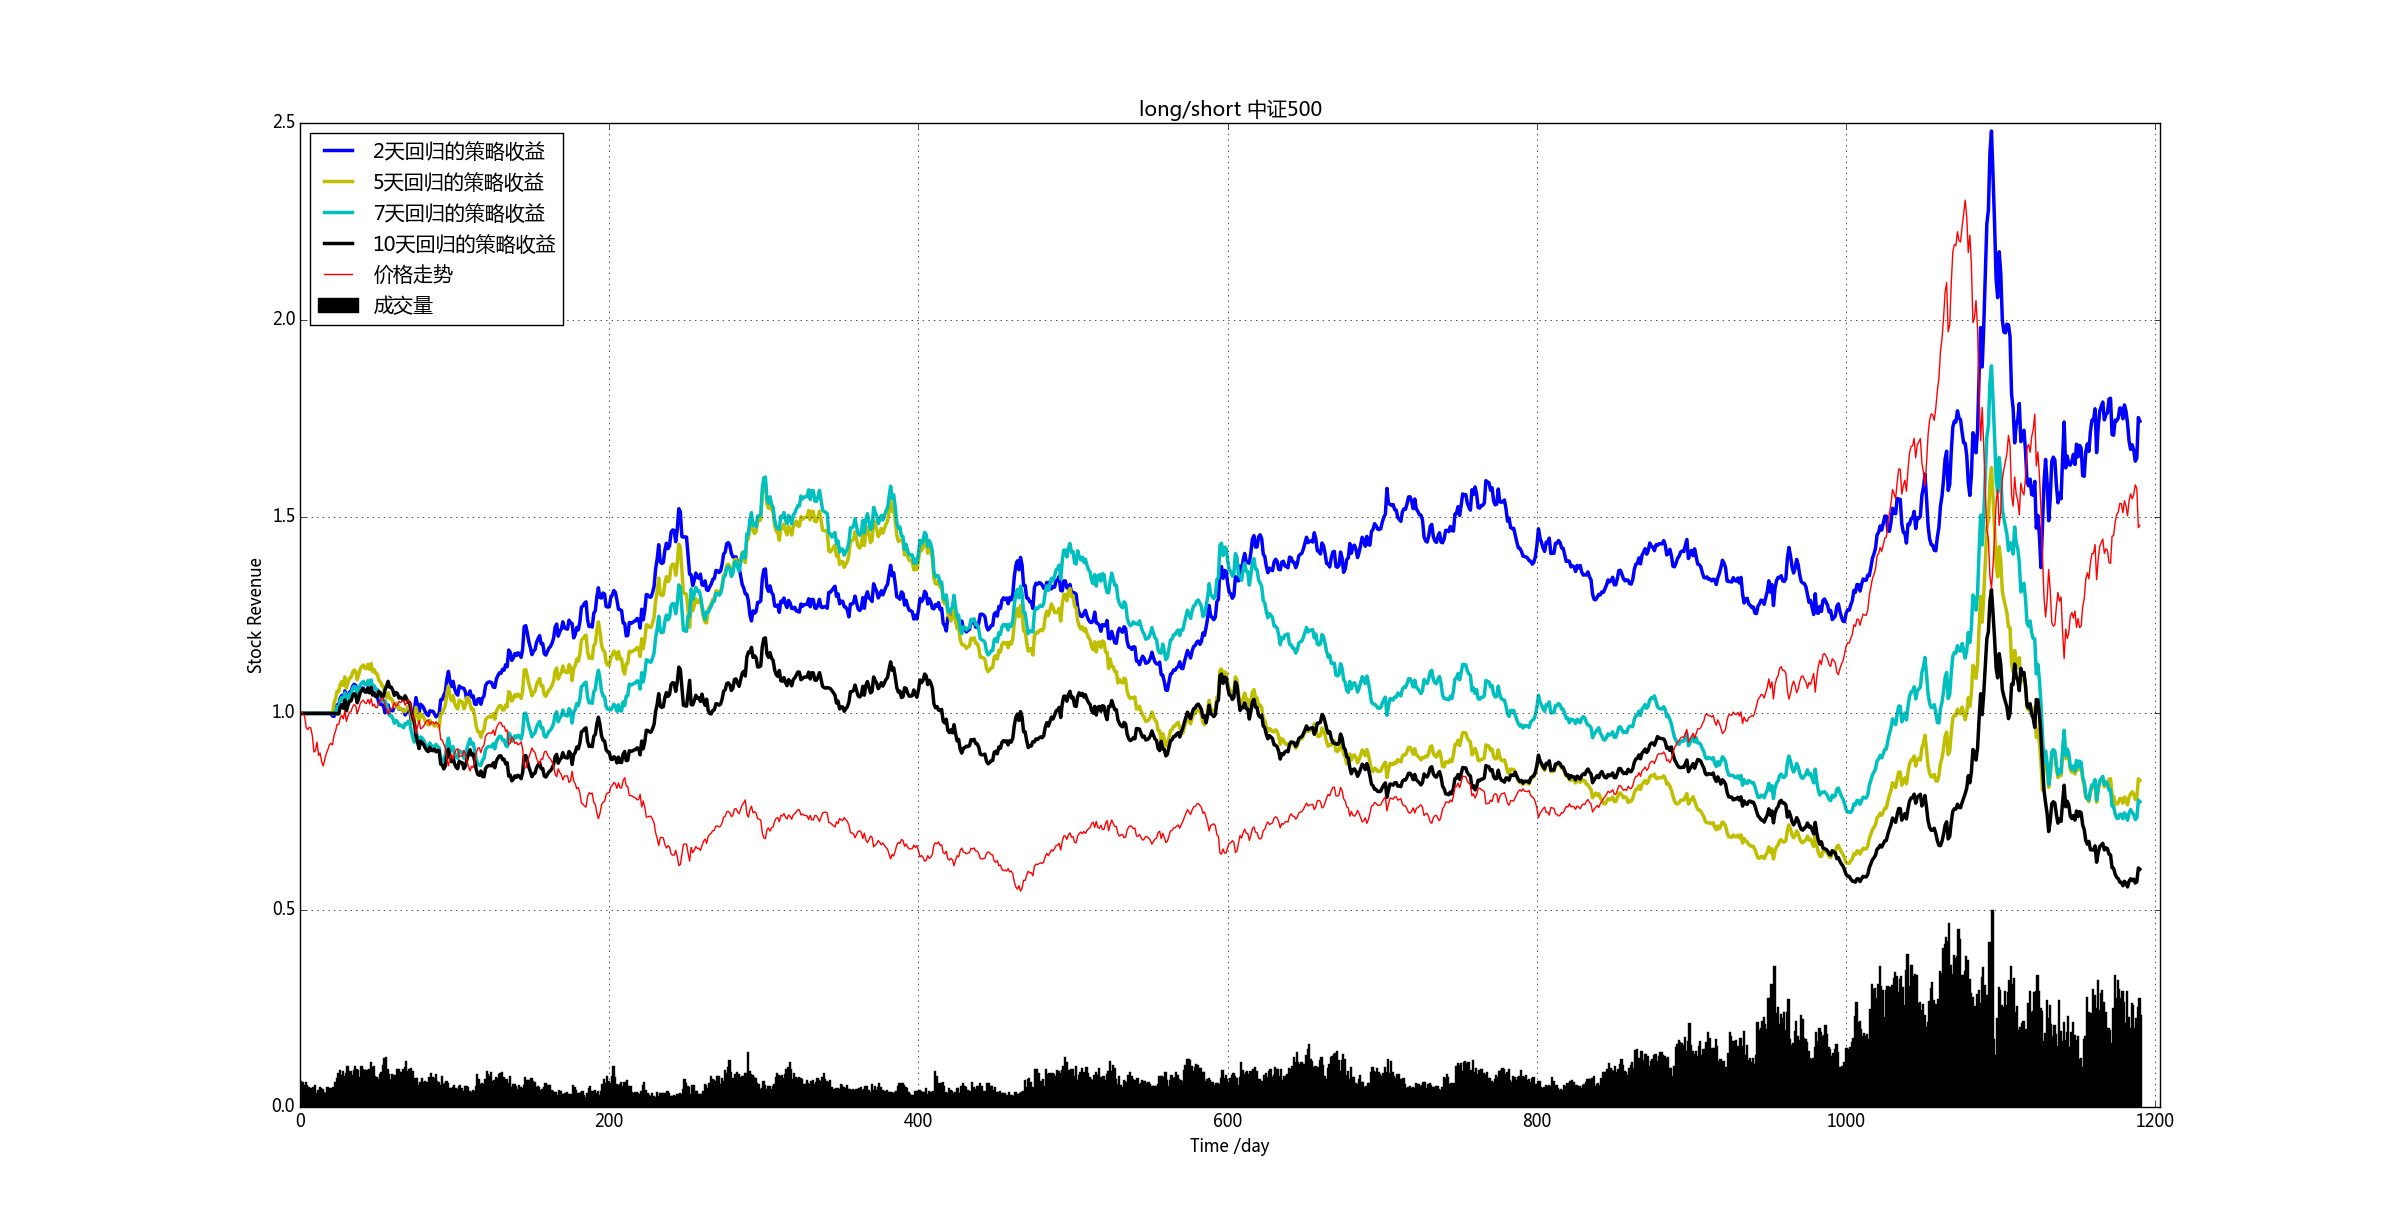
\includegraphics[width=1.0\textwidth]{img_r_10/zz500.png}
	\caption{中证500 long/short }
\end{figure}
\item long/hold 
\begin{figure}[H]
	\centering
	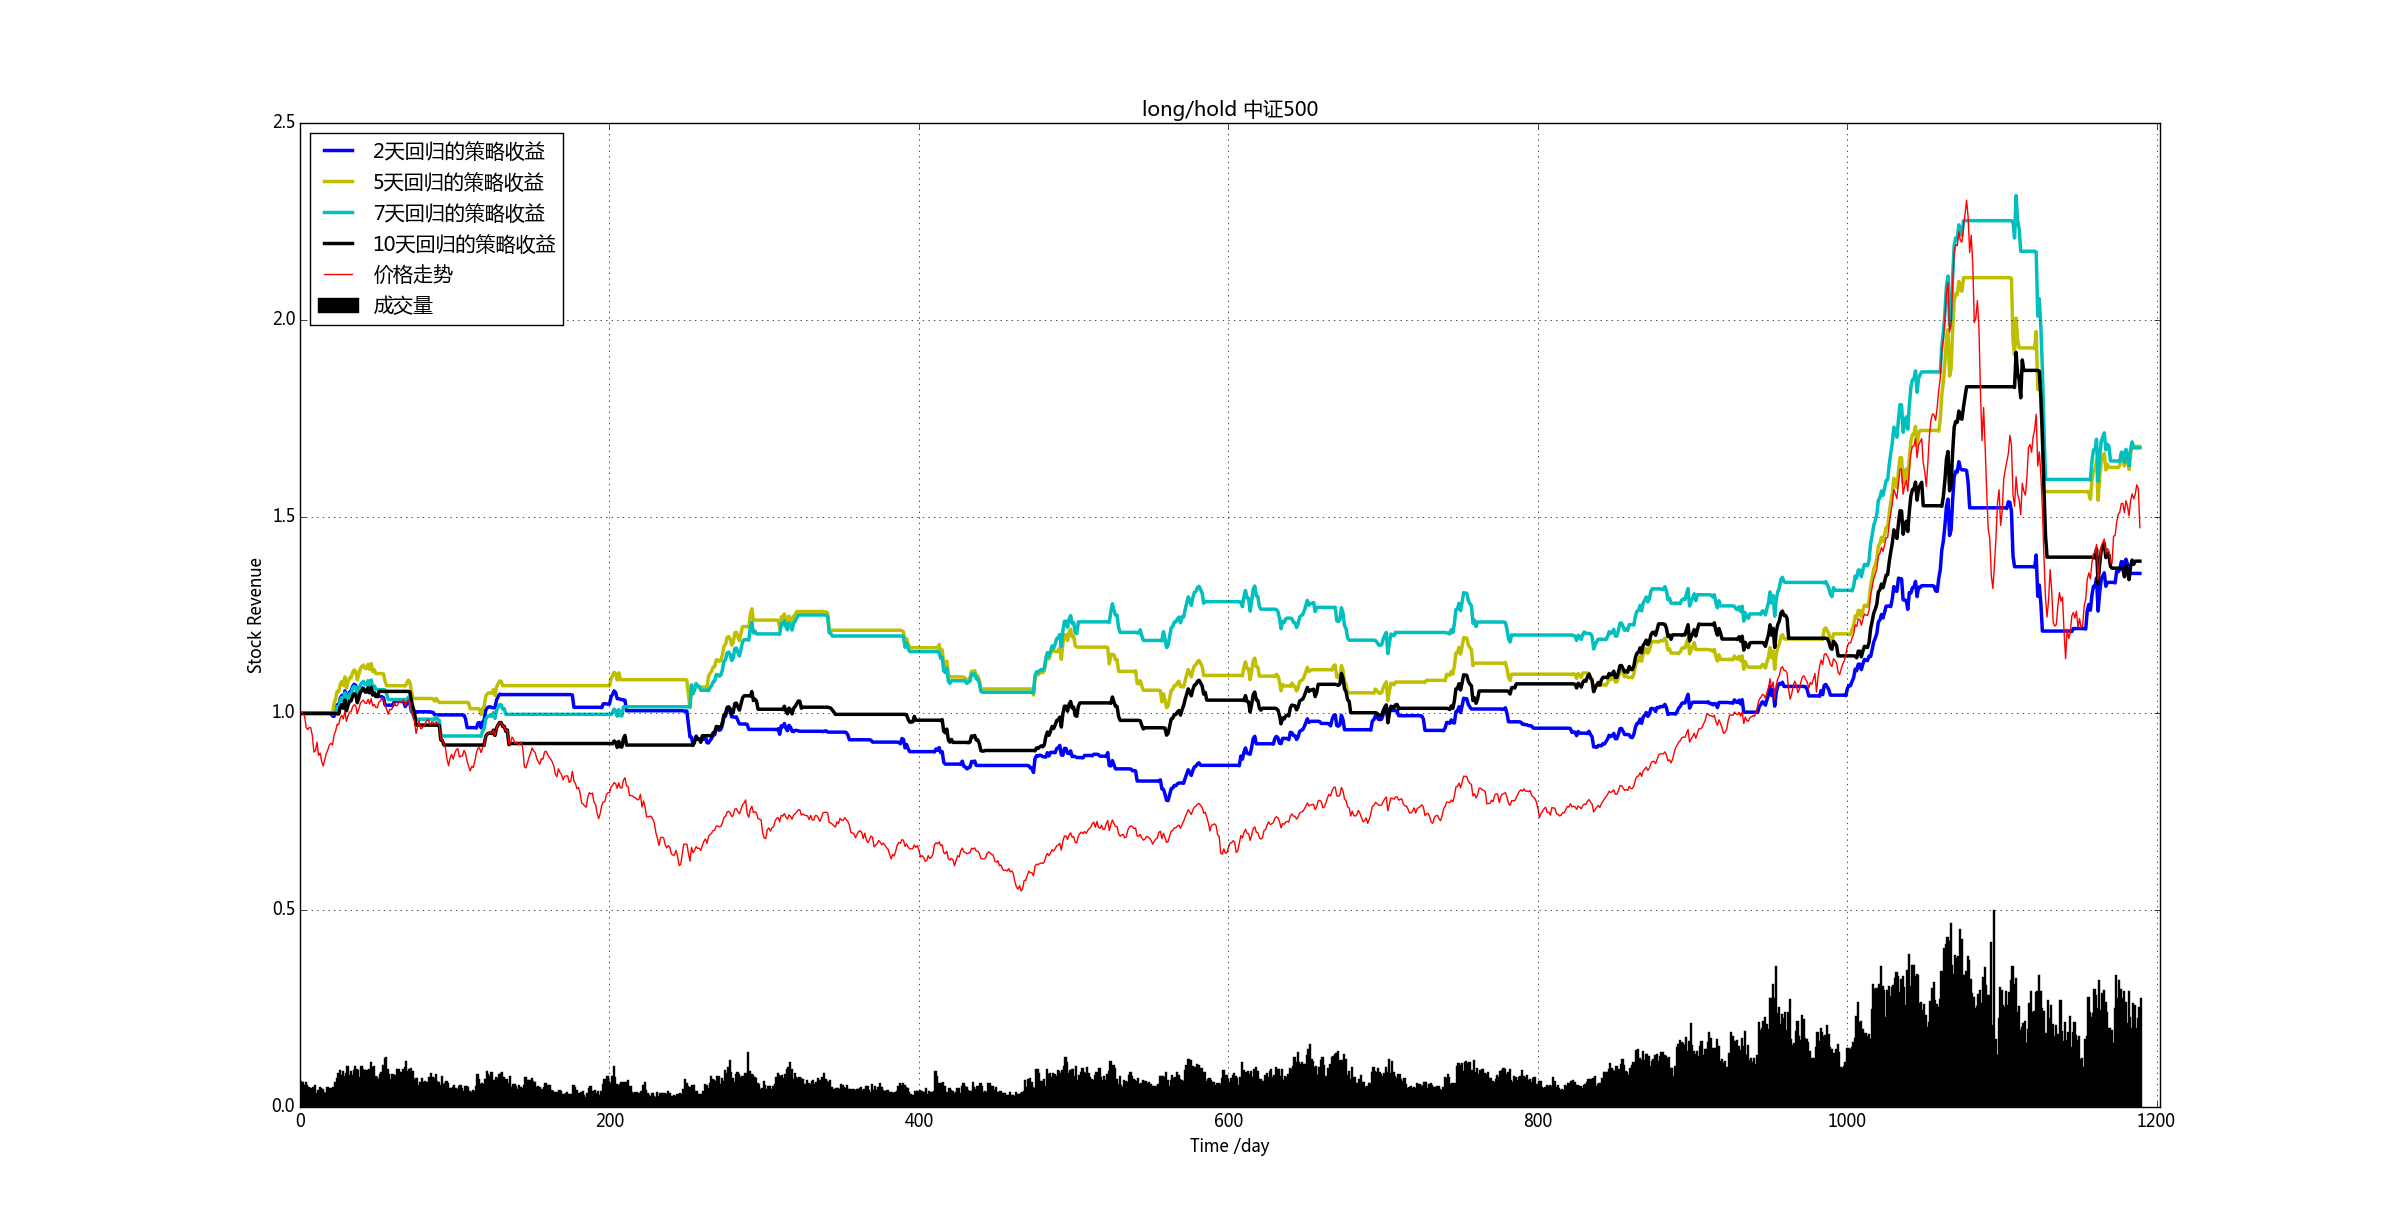
\includegraphics[width=1.0\textwidth]{img_r_10/zz500_1.png}
	\caption{中证500 long/hold}
\end{figure}
\end{enumerate}


\subsection{回测结果分析}

\begin{enumerate}
\item 从上面的各张图中可以看出,对于每个指数而言,线性回归区间为2天时,收益远远大于其他几个。线性回归区间的越短,回测收益越高。
\item 当MA的时间长度不同时,收益差别特别大。MA的时长越短,该策略的收益越高,但换手率也高。
\item 随着MA的时间长度增大,对上证50和上证综指(大盘股)的影响较小,对创业板(小盘股)的影响很大。
\item 换手率:
	\begin{enumerate}[a)]
	\item 当MA为1时,也就是不对价格和成交量进行处理时,大约每N个交易日交易一次,N是回归区间的长度,和指数的种类无关。
	\item 当MA不断增大时,交易次数会减少。举个例子,当对量价数据进行5日MA:回归区间为2天时,大约5个交易日交易一次;回归区间为10天时,大约10个交易日交易一次。
	\end{enumerate}
\item 以上几点从侧面反映了创业板(小盘股)的量价趋势很短,大都不超过3个交易日,甚至只有1、2个交易日。相对而言,主板(大盘股)的量价趋势较长,可能会有5个交易日,但也不会超过7个交易日。
\item  对比long/short 和long/hold策略,可以发现在同样的条件下,前者的performance要比后者的好。而且long/hold策略大都under-perform 。我认为原因可能是超额收益主要是由short贡献的。
\end{enumerate}




\end{document}